\documentclass[twoside]{book}

% Packages required by doxygen
\usepackage{fixltx2e}
\usepackage{calc}
\usepackage{doxygen}
\usepackage[export]{adjustbox} % also loads graphicx
\usepackage{graphicx}
\usepackage[utf8]{inputenc}
\usepackage{makeidx}
\usepackage{multicol}
\usepackage{multirow}
\PassOptionsToPackage{warn}{textcomp}
\usepackage{textcomp}
\usepackage[nointegrals]{wasysym}
\usepackage[table]{xcolor}

% Font selection
\usepackage[T1]{fontenc}
\usepackage[scaled=.90]{helvet}
\usepackage{courier}
\usepackage{amssymb}
\usepackage{sectsty}
\renewcommand{\familydefault}{\sfdefault}
\allsectionsfont{%
  \fontseries{bc}\selectfont%
  \color{darkgray}%
}
\renewcommand{\DoxyLabelFont}{%
  \fontseries{bc}\selectfont%
  \color{darkgray}%
}
\newcommand{\+}{\discretionary{\mbox{\scriptsize$\hookleftarrow$}}{}{}}

% Page & text layout
\usepackage{geometry}
\geometry{%
  a4paper,%
  top=2.5cm,%
  bottom=2.5cm,%
  left=2.5cm,%
  right=2.5cm%
}
\tolerance=750
\hfuzz=15pt
\hbadness=750
\setlength{\emergencystretch}{15pt}
\setlength{\parindent}{0cm}
\setlength{\parskip}{3ex plus 2ex minus 2ex}
\makeatletter
\renewcommand{\paragraph}{%
  \@startsection{paragraph}{4}{0ex}{-1.0ex}{1.0ex}{%
    \normalfont\normalsize\bfseries\SS@parafont%
  }%
}
\renewcommand{\subparagraph}{%
  \@startsection{subparagraph}{5}{0ex}{-1.0ex}{1.0ex}{%
    \normalfont\normalsize\bfseries\SS@subparafont%
  }%
}
\makeatother

% Headers & footers
\usepackage{fancyhdr}
\pagestyle{fancyplain}
\fancyhead[LE]{\fancyplain{}{\bfseries\thepage}}
\fancyhead[CE]{\fancyplain{}{}}
\fancyhead[RE]{\fancyplain{}{\bfseries\leftmark}}
\fancyhead[LO]{\fancyplain{}{\bfseries\rightmark}}
\fancyhead[CO]{\fancyplain{}{}}
\fancyhead[RO]{\fancyplain{}{\bfseries\thepage}}
\fancyfoot[LE]{\fancyplain{}{}}
\fancyfoot[CE]{\fancyplain{}{}}
\fancyfoot[RE]{\fancyplain{}{\bfseries\scriptsize Generated by Doxygen }}
\fancyfoot[LO]{\fancyplain{}{\bfseries\scriptsize Generated by Doxygen }}
\fancyfoot[CO]{\fancyplain{}{}}
\fancyfoot[RO]{\fancyplain{}{}}
\renewcommand{\footrulewidth}{0.4pt}
\renewcommand{\chaptermark}[1]{%
  \markboth{#1}{}%
}
\renewcommand{\sectionmark}[1]{%
  \markright{\thesection\ #1}%
}

% Indices & bibliography
\usepackage{natbib}
\usepackage[titles]{tocloft}
\setcounter{tocdepth}{3}
\setcounter{secnumdepth}{5}
\makeindex

% Hyperlinks (required, but should be loaded last)
\usepackage{ifpdf}
\ifpdf
  \usepackage[pdftex,pagebackref=true]{hyperref}
\else
  \usepackage[ps2pdf,pagebackref=true]{hyperref}
\fi
\hypersetup{%
  colorlinks=true,%
  linkcolor=blue,%
  citecolor=blue,%
  unicode%
}

% Custom commands
\newcommand{\clearemptydoublepage}{%
  \newpage{\pagestyle{empty}\cleardoublepage}%
}

\usepackage{caption}
\captionsetup{labelsep=space,justification=centering,font={bf},singlelinecheck=off,skip=4pt,position=top}

%===== C O N T E N T S =====

\begin{document}

% Titlepage & ToC
\hypersetup{pageanchor=false,
             bookmarksnumbered=true,
             pdfencoding=unicode
            }
\pagenumbering{roman}
\begin{titlepage}
\vspace*{7cm}
\begin{center}%
{\Large R\+P\+N\+Calculator }\\
\vspace*{1cm}
{\large Generated by Doxygen 1.8.11}\\
\end{center}
\end{titlepage}
\clearemptydoublepage
\tableofcontents
\clearemptydoublepage
\pagenumbering{arabic}
\hypersetup{pageanchor=true}

%--- Begin generated contents ---
\chapter{Hierarchical Index}
\section{Class Hierarchy}
This inheritance list is sorted roughly, but not completely, alphabetically\+:\begin{DoxyCompactList}
\item \contentsline{section}{Care\+Taker}{\pageref{class_care_taker}}{}
\item \contentsline{section}{Computer}{\pageref{class_computer}}{}
\item \contentsline{section}{Controller}{\pageref{class_controller}}{}
\item \contentsline{section}{Exception}{\pageref{class_exception}}{}
\begin{DoxyCompactList}
\item \contentsline{section}{Exception\+Atome}{\pageref{class_exception_atome}}{}
\item \contentsline{section}{Exception\+Empty\+Field}{\pageref{class_exception_empty_field}}{}
\item \contentsline{section}{Exception\+Memento}{\pageref{class_exception_memento}}{}
\item \contentsline{section}{Exception\+Rationnelle}{\pageref{class_exception_rationnelle}}{}
\item \contentsline{section}{Exception\+Stack}{\pageref{class_exception_stack}}{}
\item \contentsline{section}{Exception\+Syntaxte}{\pageref{class_exception_syntaxte}}{}
\item \contentsline{section}{Exception\+Wrong\+Type\+Operande}{\pageref{class_exception_wrong_type_operande}}{}
\end{DoxyCompactList}
\item \contentsline{section}{L\+T\+Atome\+Manager}{\pageref{class_l_t_atome_manager}}{}
\item \contentsline{section}{Memento}{\pageref{class_memento}}{}
\item \contentsline{section}{Operande}{\pageref{class_operande}}{}
\begin{DoxyCompactList}
\item \contentsline{section}{Litterale}{\pageref{class_litterale}}{}
\begin{DoxyCompactList}
\item \contentsline{section}{L\+T\+Expression}{\pageref{class_l_t_expression}}{}
\item \contentsline{section}{L\+T\+Programme}{\pageref{class_l_t_programme}}{}
\item \contentsline{section}{L\+T\+Sans\+Expression}{\pageref{class_l_t_sans_expression}}{}
\begin{DoxyCompactList}
\item \contentsline{section}{L\+T\+Atome}{\pageref{class_l_t_atome}}{}
\item \contentsline{section}{L\+T\+Nombre}{\pageref{class_l_t_nombre}}{}
\begin{DoxyCompactList}
\item \contentsline{section}{L\+T\+Complexe}{\pageref{class_l_t_complexe}}{}
\item \contentsline{section}{L\+T\+Numerique}{\pageref{class_l_t_numerique}}{}
\begin{DoxyCompactList}
\item \contentsline{section}{L\+T\+Entier}{\pageref{class_l_t_entier}}{}
\item \contentsline{section}{L\+T\+Rationnelle}{\pageref{class_l_t_rationnelle}}{}
\item \contentsline{section}{L\+T\+Reelle}{\pageref{class_l_t_reelle}}{}
\end{DoxyCompactList}
\end{DoxyCompactList}
\end{DoxyCompactList}
\end{DoxyCompactList}
\item \contentsline{section}{Operateur}{\pageref{class_operateur}}{}
\begin{DoxyCompactList}
\item \contentsline{section}{O\+P\+Atome}{\pageref{class_o_p_atome}}{}
\begin{DoxyCompactList}
\item \contentsline{section}{O\+P\+Forget}{\pageref{class_o_p_forget}}{}
\item \contentsline{section}{O\+P\+Sto}{\pageref{class_o_p_sto}}{}
\end{DoxyCompactList}
\item \contentsline{section}{O\+P\+Conditionnel\+Boucle}{\pageref{class_o_p_conditionnel_boucle}}{}
\begin{DoxyCompactList}
\item \contentsline{section}{O\+P\+Ift}{\pageref{class_o_p_ift}}{}
\end{DoxyCompactList}
\item \contentsline{section}{O\+P\+Literrale\+Expresion\+Programme}{\pageref{class_o_p_literrale_expresion_programme}}{}
\begin{DoxyCompactList}
\item \contentsline{section}{O\+P\+Edit}{\pageref{class_o_p_edit}}{}
\item \contentsline{section}{O\+P\+Eval}{\pageref{class_o_p_eval}}{}
\end{DoxyCompactList}
\item \contentsline{section}{O\+P\+Logique}{\pageref{class_o_p_logique}}{}
\begin{DoxyCompactList}
\item \contentsline{section}{O\+P\+And}{\pageref{class_o_p_and}}{}
\item \contentsline{section}{O\+P\+Different}{\pageref{class_o_p_different}}{}
\item \contentsline{section}{O\+P\+Egal}{\pageref{class_o_p_egal}}{}
\item \contentsline{section}{O\+P\+Inferieur}{\pageref{class_o_p_inferieur}}{}
\item \contentsline{section}{O\+P\+Inferieur\+Egal}{\pageref{class_o_p_inferieur_egal}}{}
\item \contentsline{section}{O\+P\+Not}{\pageref{class_o_p_not}}{}
\item \contentsline{section}{O\+P\+Or}{\pageref{class_o_p_or}}{}
\item \contentsline{section}{O\+P\+Superieur}{\pageref{class_o_p_superieur}}{}
\item \contentsline{section}{O\+P\+Superieur\+Egal}{\pageref{class_o_p_superieur_egal}}{}
\end{DoxyCompactList}
\item \contentsline{section}{O\+P\+Manipulation\+Pile}{\pageref{class_o_p_manipulation_pile}}{}
\begin{DoxyCompactList}
\item \contentsline{section}{O\+P\+Clear}{\pageref{class_o_p_clear}}{}
\item \contentsline{section}{O\+P\+Drop}{\pageref{class_o_p_drop}}{}
\item \contentsline{section}{O\+P\+Dup}{\pageref{class_o_p_dup}}{}
\item \contentsline{section}{O\+P\+Last\+Args}{\pageref{class_o_p_last_args}}{}
\item \contentsline{section}{O\+P\+Last\+Op}{\pageref{class_o_p_last_op}}{}
\item \contentsline{section}{O\+P\+Redo}{\pageref{class_o_p_redo}}{}
\item \contentsline{section}{O\+P\+Swap}{\pageref{class_o_p_swap}}{}
\item \contentsline{section}{O\+P\+Undo}{\pageref{class_o_p_undo}}{}
\end{DoxyCompactList}
\item \contentsline{section}{O\+P\+Numerique}{\pageref{class_o_p_numerique}}{}
\begin{DoxyCompactList}
\item \contentsline{section}{O\+P\+Addition}{\pageref{class_o_p_addition}}{}
\item \contentsline{section}{O\+P\+Complexe}{\pageref{class_o_p_complexe}}{}
\item \contentsline{section}{O\+P\+Denominateur}{\pageref{class_o_p_denominateur}}{}
\item \contentsline{section}{O\+P\+Division}{\pageref{class_o_p_division}}{}
\item \contentsline{section}{O\+P\+Division\+Entiere}{\pageref{class_o_p_division_entiere}}{}
\item \contentsline{section}{O\+P\+Modulo}{\pageref{class_o_p_modulo}}{}
\item \contentsline{section}{O\+P\+Multiplication}{\pageref{class_o_p_multiplication}}{}
\item \contentsline{section}{O\+P\+Negation}{\pageref{class_o_p_negation}}{}
\item \contentsline{section}{O\+P\+Numerateur}{\pageref{class_o_p_numerateur}}{}
\item \contentsline{section}{O\+P\+Partie\+Imaginaire\+Complexe}{\pageref{class_o_p_partie_imaginaire_complexe}}{}
\item \contentsline{section}{O\+P\+Partie\+Reelle\+Complexe}{\pageref{class_o_p_partie_reelle_complexe}}{}
\item \contentsline{section}{O\+P\+Soustraction}{\pageref{class_o_p_soustraction}}{}
\end{DoxyCompactList}
\end{DoxyCompactList}
\item \contentsline{section}{O\+P\+Num\+\_\+\+L\+T\+Sans\+Expression}{\pageref{class_o_p_num___l_t_sans_expression}}{}
\begin{DoxyCompactList}
\item \contentsline{section}{L\+T\+Sans\+Expression}{\pageref{class_l_t_sans_expression}}{}
\item \contentsline{section}{O\+P\+Numerique}{\pageref{class_o_p_numerique}}{}
\end{DoxyCompactList}
\end{DoxyCompactList}
\item \contentsline{section}{Operande\+Factory}{\pageref{class_operande_factory}}{}
\item \contentsline{section}{Originator}{\pageref{class_originator}}{}
\item \contentsline{section}{Parseur}{\pageref{class_parseur}}{}
\item Q\+H\+Box\+Layout\begin{DoxyCompactList}
\item \contentsline{section}{U\+I\+Buttons\+Line}{\pageref{class_u_i_buttons_line}}{}
\end{DoxyCompactList}
\item Q\+Line\+Edit\begin{DoxyCompactList}
\item \contentsline{section}{U\+I\+Command\+Line}{\pageref{class_u_i_command_line}}{}
\end{DoxyCompactList}
\item Q\+Main\+Window\begin{DoxyCompactList}
\item \contentsline{section}{U\+I\+Create\+Var\+Window}{\pageref{class_u_i_create_var_window}}{}
\item \contentsline{section}{U\+I\+Prog\+Editor}{\pageref{class_u_i_prog_editor}}{}
\item \contentsline{section}{U\+I\+Setting\+Window}{\pageref{class_u_i_setting_window}}{}
\item \contentsline{section}{U\+I\+Text\+Editor}{\pageref{class_u_i_text_editor}}{}
\item \contentsline{section}{U\+I\+Var\+Editor}{\pageref{class_u_i_var_editor}}{}
\item \contentsline{section}{U\+T\+Computer}{\pageref{class_u_t_computer}}{}
\end{DoxyCompactList}
\item Q\+Push\+Button\begin{DoxyCompactList}
\item \contentsline{section}{U\+I\+Button}{\pageref{class_u_i_button}}{}
\end{DoxyCompactList}
\item Q\+Table\+Widget\begin{DoxyCompactList}
\item \contentsline{section}{U\+I\+Pile\+Var\+View}{\pageref{class_u_i_pile_var_view}}{}
\item \contentsline{section}{U\+I\+Pile\+View}{\pageref{class_u_i_pile_view}}{}
\end{DoxyCompactList}
\item Q\+Text\+Edit\begin{DoxyCompactList}
\item \contentsline{section}{U\+I\+Message\+Line}{\pageref{class_u_i_message_line}}{}
\end{DoxyCompactList}
\item Q\+V\+Box\+Layout\begin{DoxyCompactList}
\item \contentsline{section}{U\+I\+Keyboard\+Layout}{\pageref{class_u_i_keyboard_layout}}{}
\end{DoxyCompactList}
\item Q\+Widget\begin{DoxyCompactList}
\item \contentsline{section}{U\+I\+Keyboard}{\pageref{class_u_i_keyboard}}{}
\item \contentsline{section}{U\+I\+Menu}{\pageref{class_u_i_menu}}{}
\end{DoxyCompactList}
\item \contentsline{section}{Stack}{\pageref{class_stack}}{}
\item \contentsline{section}{X\+M\+L\+Manager}{\pageref{class_x_m_l_manager}}{}
\end{DoxyCompactList}

\chapter{Class Index}
\section{Class List}
Here are the classes, structs, unions and interfaces with brief descriptions\+:\begin{DoxyCompactList}
\item\contentsline{section}{\hyperlink{class_care_taker}{Care\+Taker} }{\pageref{class_care_taker}}{}
\item\contentsline{section}{\hyperlink{class_computer}{Computer} \\*La classe \hyperlink{class_computer}{Computer} est un singleton qui s\textquotesingle{}occupe du calcul des litterales avec un opérateur $\ast$/ }{\pageref{class_computer}}{}
\item\contentsline{section}{\hyperlink{class_controller}{Controller} \\*Classe du controller \+: il gère l\textquotesingle{}ensemble de la partie calculatoire de la calculatrice }{\pageref{class_controller}}{}
\item\contentsline{section}{\hyperlink{class_exception}{Exception} \\*Classe mère abstraite pour gérer les exceptions }{\pageref{class_exception}}{}
\item\contentsline{section}{\hyperlink{class_exception_atome}{Exception\+Atome} \\*Classe d\textquotesingle{}exception pour les Litterales Atomes }{\pageref{class_exception_atome}}{}
\item\contentsline{section}{\hyperlink{class_exception_empty_field}{Exception\+Empty\+Field} \\*Classe d\textquotesingle{}exception pour les vérifications des champs }{\pageref{class_exception_empty_field}}{}
\item\contentsline{section}{\hyperlink{class_exception_memento}{Exception\+Memento} \\*Classe d\textquotesingle{}exception pour le design pattern \hyperlink{class_memento}{Memento} et la gestion de l\textquotesingle{}Undo Redo }{\pageref{class_exception_memento}}{}
\item\contentsline{section}{\hyperlink{class_exception_rationnelle}{Exception\+Rationnelle} \\*Classe d\textquotesingle{}exception pour les Litterales Rationnelles }{\pageref{class_exception_rationnelle}}{}
\item\contentsline{section}{\hyperlink{class_exception_stack}{Exception\+Stack} \\*Classe d\textquotesingle{}exception de la pile }{\pageref{class_exception_stack}}{}
\item\contentsline{section}{\hyperlink{class_exception_syntaxte}{Exception\+Syntaxte} \\*Classe d\textquotesingle{}exception pour la syntaxe }{\pageref{class_exception_syntaxte}}{}
\item\contentsline{section}{\hyperlink{class_exception_wrong_type_operande}{Exception\+Wrong\+Type\+Operande} \\*Classe d\textquotesingle{}exception si une opérande est mal utilisée }{\pageref{class_exception_wrong_type_operande}}{}
\item\contentsline{section}{\hyperlink{class_litterale}{Litterale} \\*Classe mère de toutes les litterales (abstraite) }{\pageref{class_litterale}}{}
\item\contentsline{section}{\hyperlink{class_l_t_atome}{L\+T\+Atome} \\*Classe d\textquotesingle{}une litterale atome }{\pageref{class_l_t_atome}}{}
\item\contentsline{section}{\hyperlink{class_l_t_atome_manager}{L\+T\+Atome\+Manager} \\*Classe \hyperlink{class_l_t_atome_manager}{L\+T\+Atome\+Manager} (Singleton) \+: factory d\textquotesingle{}atome, gère leur création, notamment les cas où un atome du même nom existe déjà }{\pageref{class_l_t_atome_manager}}{}
\item\contentsline{section}{\hyperlink{class_l_t_complexe}{L\+T\+Complexe} \\*Classe gérant les nombres complexes }{\pageref{class_l_t_complexe}}{}
\item\contentsline{section}{\hyperlink{class_l_t_entier}{L\+T\+Entier} }{\pageref{class_l_t_entier}}{}
\item\contentsline{section}{\hyperlink{class_l_t_expression}{L\+T\+Expression} \\*Classe \hyperlink{class_l_t_expression}{L\+T\+Expression}, gérant les expressions }{\pageref{class_l_t_expression}}{}
\item\contentsline{section}{\hyperlink{class_l_t_nombre}{L\+T\+Nombre} \\*Classe \hyperlink{class_l_t_nombre}{L\+T\+Nombre} abstraite }{\pageref{class_l_t_nombre}}{}
\item\contentsline{section}{\hyperlink{class_l_t_numerique}{L\+T\+Numerique} }{\pageref{class_l_t_numerique}}{}
\item\contentsline{section}{\hyperlink{class_l_t_programme}{L\+T\+Programme} }{\pageref{class_l_t_programme}}{}
\item\contentsline{section}{\hyperlink{class_l_t_rationnelle}{L\+T\+Rationnelle} }{\pageref{class_l_t_rationnelle}}{}
\item\contentsline{section}{\hyperlink{class_l_t_reelle}{L\+T\+Reelle} }{\pageref{class_l_t_reelle}}{}
\item\contentsline{section}{\hyperlink{class_l_t_sans_expression}{L\+T\+Sans\+Expression} }{\pageref{class_l_t_sans_expression}}{}
\item\contentsline{section}{\hyperlink{class_memento}{Memento} }{\pageref{class_memento}}{}
\item\contentsline{section}{\hyperlink{class_o_p_addition}{O\+P\+Addition} }{\pageref{class_o_p_addition}}{}
\item\contentsline{section}{\hyperlink{class_o_p_and}{O\+P\+And} }{\pageref{class_o_p_and}}{}
\item\contentsline{section}{\hyperlink{class_o_p_atome}{O\+P\+Atome} }{\pageref{class_o_p_atome}}{}
\item\contentsline{section}{\hyperlink{class_o_p_clear}{O\+P\+Clear} }{\pageref{class_o_p_clear}}{}
\item\contentsline{section}{\hyperlink{class_o_p_complexe}{O\+P\+Complexe} }{\pageref{class_o_p_complexe}}{}
\item\contentsline{section}{\hyperlink{class_o_p_conditionnel_boucle}{O\+P\+Conditionnel\+Boucle} }{\pageref{class_o_p_conditionnel_boucle}}{}
\item\contentsline{section}{\hyperlink{class_o_p_denominateur}{O\+P\+Denominateur} }{\pageref{class_o_p_denominateur}}{}
\item\contentsline{section}{\hyperlink{class_o_p_different}{O\+P\+Different} }{\pageref{class_o_p_different}}{}
\item\contentsline{section}{\hyperlink{class_o_p_division}{O\+P\+Division} }{\pageref{class_o_p_division}}{}
\item\contentsline{section}{\hyperlink{class_o_p_division_entiere}{O\+P\+Division\+Entiere} }{\pageref{class_o_p_division_entiere}}{}
\item\contentsline{section}{\hyperlink{class_o_p_drop}{O\+P\+Drop} }{\pageref{class_o_p_drop}}{}
\item\contentsline{section}{\hyperlink{class_o_p_dup}{O\+P\+Dup} }{\pageref{class_o_p_dup}}{}
\item\contentsline{section}{\hyperlink{class_o_p_edit}{O\+P\+Edit} }{\pageref{class_o_p_edit}}{}
\item\contentsline{section}{\hyperlink{class_o_p_egal}{O\+P\+Egal} }{\pageref{class_o_p_egal}}{}
\item\contentsline{section}{\hyperlink{class_operande}{Operande} }{\pageref{class_operande}}{}
\item\contentsline{section}{\hyperlink{class_operande_factory}{Operande\+Factory} }{\pageref{class_operande_factory}}{}
\item\contentsline{section}{\hyperlink{class_operateur}{Operateur} }{\pageref{class_operateur}}{}
\item\contentsline{section}{\hyperlink{class_o_p_eval}{O\+P\+Eval} }{\pageref{class_o_p_eval}}{}
\item\contentsline{section}{\hyperlink{class_o_p_forget}{O\+P\+Forget} }{\pageref{class_o_p_forget}}{}
\item\contentsline{section}{\hyperlink{class_o_p_ift}{O\+P\+Ift} }{\pageref{class_o_p_ift}}{}
\item\contentsline{section}{\hyperlink{class_o_p_inferieur}{O\+P\+Inferieur} }{\pageref{class_o_p_inferieur}}{}
\item\contentsline{section}{\hyperlink{class_o_p_inferieur_egal}{O\+P\+Inferieur\+Egal} }{\pageref{class_o_p_inferieur_egal}}{}
\item\contentsline{section}{\hyperlink{class_o_p_last_args}{O\+P\+Last\+Args} }{\pageref{class_o_p_last_args}}{}
\item\contentsline{section}{\hyperlink{class_o_p_last_op}{O\+P\+Last\+Op} }{\pageref{class_o_p_last_op}}{}
\item\contentsline{section}{\hyperlink{class_o_p_literrale_expresion_programme}{O\+P\+Literrale\+Expresion\+Programme} }{\pageref{class_o_p_literrale_expresion_programme}}{}
\item\contentsline{section}{\hyperlink{class_o_p_logique}{O\+P\+Logique} }{\pageref{class_o_p_logique}}{}
\item\contentsline{section}{\hyperlink{class_o_p_manipulation_pile}{O\+P\+Manipulation\+Pile} }{\pageref{class_o_p_manipulation_pile}}{}
\item\contentsline{section}{\hyperlink{class_o_p_modulo}{O\+P\+Modulo} }{\pageref{class_o_p_modulo}}{}
\item\contentsline{section}{\hyperlink{class_o_p_multiplication}{O\+P\+Multiplication} }{\pageref{class_o_p_multiplication}}{}
\item\contentsline{section}{\hyperlink{class_o_p_negation}{O\+P\+Negation} }{\pageref{class_o_p_negation}}{}
\item\contentsline{section}{\hyperlink{class_o_p_not}{O\+P\+Not} }{\pageref{class_o_p_not}}{}
\item\contentsline{section}{\hyperlink{class_o_p_num___l_t_sans_expression}{O\+P\+Num\+\_\+\+L\+T\+Sans\+Expression} }{\pageref{class_o_p_num___l_t_sans_expression}}{}
\item\contentsline{section}{\hyperlink{class_o_p_numerateur}{O\+P\+Numerateur} }{\pageref{class_o_p_numerateur}}{}
\item\contentsline{section}{\hyperlink{class_o_p_numerique}{O\+P\+Numerique} }{\pageref{class_o_p_numerique}}{}
\item\contentsline{section}{\hyperlink{class_o_p_or}{O\+P\+Or} }{\pageref{class_o_p_or}}{}
\item\contentsline{section}{\hyperlink{class_o_p_partie_imaginaire_complexe}{O\+P\+Partie\+Imaginaire\+Complexe} }{\pageref{class_o_p_partie_imaginaire_complexe}}{}
\item\contentsline{section}{\hyperlink{class_o_p_partie_reelle_complexe}{O\+P\+Partie\+Reelle\+Complexe} }{\pageref{class_o_p_partie_reelle_complexe}}{}
\item\contentsline{section}{\hyperlink{class_o_p_redo}{O\+P\+Redo} }{\pageref{class_o_p_redo}}{}
\item\contentsline{section}{\hyperlink{class_o_p_soustraction}{O\+P\+Soustraction} }{\pageref{class_o_p_soustraction}}{}
\item\contentsline{section}{\hyperlink{class_o_p_sto}{O\+P\+Sto} }{\pageref{class_o_p_sto}}{}
\item\contentsline{section}{\hyperlink{class_o_p_superieur}{O\+P\+Superieur} }{\pageref{class_o_p_superieur}}{}
\item\contentsline{section}{\hyperlink{class_o_p_superieur_egal}{O\+P\+Superieur\+Egal} }{\pageref{class_o_p_superieur_egal}}{}
\item\contentsline{section}{\hyperlink{class_o_p_swap}{O\+P\+Swap} }{\pageref{class_o_p_swap}}{}
\item\contentsline{section}{\hyperlink{class_o_p_undo}{O\+P\+Undo} }{\pageref{class_o_p_undo}}{}
\item\contentsline{section}{\hyperlink{class_originator}{Originator} }{\pageref{class_originator}}{}
\item\contentsline{section}{\hyperlink{class_parseur}{Parseur} }{\pageref{class_parseur}}{}
\item\contentsline{section}{\hyperlink{class_stack}{Stack} }{\pageref{class_stack}}{}
\item\contentsline{section}{\hyperlink{class_u_i_button}{U\+I\+Button} }{\pageref{class_u_i_button}}{}
\item\contentsline{section}{\hyperlink{class_u_i_buttons_line}{U\+I\+Buttons\+Line} }{\pageref{class_u_i_buttons_line}}{}
\item\contentsline{section}{\hyperlink{class_u_i_command_line}{U\+I\+Command\+Line} }{\pageref{class_u_i_command_line}}{}
\item\contentsline{section}{\hyperlink{class_u_i_create_var_window}{U\+I\+Create\+Var\+Window} }{\pageref{class_u_i_create_var_window}}{}
\item\contentsline{section}{\hyperlink{class_u_i_keyboard}{U\+I\+Keyboard} }{\pageref{class_u_i_keyboard}}{}
\item\contentsline{section}{\hyperlink{class_u_i_keyboard_layout}{U\+I\+Keyboard\+Layout} }{\pageref{class_u_i_keyboard_layout}}{}
\item\contentsline{section}{\hyperlink{class_u_i_menu}{U\+I\+Menu} }{\pageref{class_u_i_menu}}{}
\item\contentsline{section}{\hyperlink{class_u_i_message_line}{U\+I\+Message\+Line} }{\pageref{class_u_i_message_line}}{}
\item\contentsline{section}{\hyperlink{class_u_i_pile_var_view}{U\+I\+Pile\+Var\+View} }{\pageref{class_u_i_pile_var_view}}{}
\item\contentsline{section}{\hyperlink{class_u_i_pile_view}{U\+I\+Pile\+View} }{\pageref{class_u_i_pile_view}}{}
\item\contentsline{section}{\hyperlink{class_u_i_prog_editor}{U\+I\+Prog\+Editor} }{\pageref{class_u_i_prog_editor}}{}
\item\contentsline{section}{\hyperlink{class_u_i_setting_window}{U\+I\+Setting\+Window} }{\pageref{class_u_i_setting_window}}{}
\item\contentsline{section}{\hyperlink{class_u_i_text_editor}{U\+I\+Text\+Editor} }{\pageref{class_u_i_text_editor}}{}
\item\contentsline{section}{\hyperlink{class_u_i_var_editor}{U\+I\+Var\+Editor} }{\pageref{class_u_i_var_editor}}{}
\item\contentsline{section}{\hyperlink{class_u_t_computer}{U\+T\+Computer} }{\pageref{class_u_t_computer}}{}
\item\contentsline{section}{\hyperlink{class_x_m_l_manager}{X\+M\+L\+Manager} }{\pageref{class_x_m_l_manager}}{}
\end{DoxyCompactList}

\chapter{Class Documentation}
\hypertarget{class_care_taker}{}\section{Care\+Taker Class Reference}
\label{class_care_taker}\index{Care\+Taker@{Care\+Taker}}
\subsection*{Public Member Functions}
\begin{DoxyCompactItemize}
\item 
void {\bfseries add\+Memento} (\hyperlink{class_memento}{Memento} m, int index)\hypertarget{class_care_taker_af68e1bd6a333e599aadfc67868a67218}{}\label{class_care_taker_af68e1bd6a333e599aadfc67868a67218}

\item 
\hyperlink{class_memento}{Memento} {\bfseries get\+Memento} (int index)\hypertarget{class_care_taker_a61a5e9d7f1bc650b1b8cba22368fb32c}{}\label{class_care_taker_a61a5e9d7f1bc650b1b8cba22368fb32c}

\item 
int {\bfseries size} ()\hypertarget{class_care_taker_a0588647afc65bba97a7387b013122889}{}\label{class_care_taker_a0588647afc65bba97a7387b013122889}

\end{DoxyCompactItemize}


The documentation for this class was generated from the following file\+:\begin{DoxyCompactItemize}
\item 
memento.\+h\end{DoxyCompactItemize}

\hypertarget{class_computer}{}\section{Computer Class Reference}
\label{class_computer}\index{Computer@{Computer}}


La classe \hyperlink{class_computer}{Computer} est un singleton qui s\textquotesingle{}occupe du calcul des litterales avec un opérateur $\ast$/.  




{\ttfamily \#include $<$computer.\+h$>$}

\subsection*{Public Member Functions}
\begin{DoxyCompactItemize}
\item 
\hyperlink{class_litterale}{Litterale} $\ast$ \hyperlink{class_computer_a0abcb800a1983fa735ead34f569b9e51}{compute} (\hyperlink{class_operateur}{Operateur} $\ast$op)
\begin{DoxyCompactList}\small\item\em Méthode qui permet d\textquotesingle{}appliquer un opérateur, ne prennant aucun paramètre. \end{DoxyCompactList}\item 
\hyperlink{class_litterale}{Litterale} $\ast$ \hyperlink{class_computer_abb4f32bacba91222d6d98a696af0c401}{compute} (\hyperlink{class_operateur}{Operateur} $\ast$op, \hyperlink{class_litterale}{Litterale} $\ast$l1)
\begin{DoxyCompactList}\small\item\em Méthode qui permet d\textquotesingle{}appliquer un opérateur, s\textquotesingle{}appliquant sur un paramètre. \end{DoxyCompactList}\item 
\hyperlink{class_litterale}{Litterale} $\ast$ \hyperlink{class_computer_a016bf583f6ec6d1c1c71ed9246ecc5bb}{compute} (\hyperlink{class_operateur}{Operateur} $\ast$op, \hyperlink{class_litterale}{Litterale} $\ast$l1, \hyperlink{class_litterale}{Litterale} $\ast$l2)
\begin{DoxyCompactList}\small\item\em Méthode qui permet d\textquotesingle{}appliquer un opérateur, s\textquotesingle{}appliquant sur 2 paramètres. \end{DoxyCompactList}\item 
\hyperlink{class_operateur}{Operateur} $\ast$ \hyperlink{class_computer_a7cb35cf9cdf9f0a89328501a8cbd46dc}{get\+Last\+Op} ()
\begin{DoxyCompactList}\small\item\em Permet de récupérer le dernier opérateur utilisé \end{DoxyCompactList}\item 
Q\+List$<$ \hyperlink{class_litterale}{Litterale} $\ast$ $>$ $\ast$ \hyperlink{class_computer_a3804a17a6441a746b06a79000f03aacb}{get\+Last\+Args} ()
\begin{DoxyCompactList}\small\item\em Méthode qui permet de récupérer les dernières litterales utilisées avec le dernier opérateur. \end{DoxyCompactList}\end{DoxyCompactItemize}
\subsection*{Static Public Member Functions}
\begin{DoxyCompactItemize}
\item 
static \hyperlink{class_computer}{Computer} \& \hyperlink{class_computer_ad102422d1f9a9b8a5537743571956906}{get\+Instance} ()
\begin{DoxyCompactList}\small\item\em Getter de l\textquotesingle{}instance du singleton. \end{DoxyCompactList}\item 
static void \hyperlink{class_computer_a9774870a8cc9fadfa5137c11ebbb70cf}{free\+Instance} ()\hypertarget{class_computer_a9774870a8cc9fadfa5137c11ebbb70cf}{}\label{class_computer_a9774870a8cc9fadfa5137c11ebbb70cf}

\begin{DoxyCompactList}\small\item\em Destructeur de l\textquotesingle{}instance du singleton. \end{DoxyCompactList}\end{DoxyCompactItemize}


\subsection{Detailed Description}
La classe \hyperlink{class_computer}{Computer} est un singleton qui s\textquotesingle{}occupe du calcul des litterales avec un opérateur $\ast$/. 

\subsection{Member Function Documentation}
\index{Computer@{Computer}!compute@{compute}}
\index{compute@{compute}!Computer@{Computer}}
\subsubsection[{\texorpdfstring{compute(\+Operateur $\ast$op)}{compute(Operateur *op)}}]{\setlength{\rightskip}{0pt plus 5cm}{\bf Litterale} $\ast$ Computer\+::compute (
\begin{DoxyParamCaption}
\item[{{\bf Operateur} $\ast$}]{op}
\end{DoxyParamCaption}
)}\hypertarget{class_computer_a0abcb800a1983fa735ead34f569b9e51}{}\label{class_computer_a0abcb800a1983fa735ead34f569b9e51}


Méthode qui permet d\textquotesingle{}appliquer un opérateur, ne prennant aucun paramètre. 


\begin{DoxyParams}{Parameters}
{\em op} & Opérateur à appliquer \\
\hline
\end{DoxyParams}
\begin{DoxyReturn}{Returns}
Littérale résultat 
\end{DoxyReturn}
\index{Computer@{Computer}!compute@{compute}}
\index{compute@{compute}!Computer@{Computer}}
\subsubsection[{\texorpdfstring{compute(\+Operateur $\ast$op, Litterale $\ast$l1)}{compute(Operateur *op, Litterale *l1)}}]{\setlength{\rightskip}{0pt plus 5cm}{\bf Litterale} $\ast$ Computer\+::compute (
\begin{DoxyParamCaption}
\item[{{\bf Operateur} $\ast$}]{op, }
\item[{{\bf Litterale} $\ast$}]{l1}
\end{DoxyParamCaption}
)}\hypertarget{class_computer_abb4f32bacba91222d6d98a696af0c401}{}\label{class_computer_abb4f32bacba91222d6d98a696af0c401}


Méthode qui permet d\textquotesingle{}appliquer un opérateur, s\textquotesingle{}appliquant sur un paramètre. 


\begin{DoxyParams}{Parameters}
{\em op} & Opérateur à appliquer \\
\hline
{\em l1} & Littérale sur lequel l\textquotesingle{}opérateur s\textquotesingle{}applique \\
\hline
\end{DoxyParams}
\begin{DoxyReturn}{Returns}
Littérale résultat 
\end{DoxyReturn}
\index{Computer@{Computer}!compute@{compute}}
\index{compute@{compute}!Computer@{Computer}}
\subsubsection[{\texorpdfstring{compute(\+Operateur $\ast$op, Litterale $\ast$l1, Litterale $\ast$l2)}{compute(Operateur *op, Litterale *l1, Litterale *l2)}}]{\setlength{\rightskip}{0pt plus 5cm}{\bf Litterale} $\ast$ Computer\+::compute (
\begin{DoxyParamCaption}
\item[{{\bf Operateur} $\ast$}]{op, }
\item[{{\bf Litterale} $\ast$}]{l1, }
\item[{{\bf Litterale} $\ast$}]{l2}
\end{DoxyParamCaption}
)}\hypertarget{class_computer_a016bf583f6ec6d1c1c71ed9246ecc5bb}{}\label{class_computer_a016bf583f6ec6d1c1c71ed9246ecc5bb}


Méthode qui permet d\textquotesingle{}appliquer un opérateur, s\textquotesingle{}appliquant sur 2 paramètres. 


\begin{DoxyParams}{Parameters}
{\em op} & Opérateur à appliquer \\
\hline
{\em l1} & Littérale sur lequel l\textquotesingle{}opérateur s\textquotesingle{}applique \\
\hline
{\em l2} & Littérale sur lequel l\textquotesingle{}opérateur s\textquotesingle{}applique \\
\hline
\end{DoxyParams}
\begin{DoxyReturn}{Returns}
Littérale résultat 
\end{DoxyReturn}
\index{Computer@{Computer}!get\+Instance@{get\+Instance}}
\index{get\+Instance@{get\+Instance}!Computer@{Computer}}
\subsubsection[{\texorpdfstring{get\+Instance()}{getInstance()}}]{\setlength{\rightskip}{0pt plus 5cm}static {\bf Computer}\& Computer\+::get\+Instance (
\begin{DoxyParamCaption}
{}
\end{DoxyParamCaption}
)\hspace{0.3cm}{\ttfamily [inline]}, {\ttfamily [static]}}\hypertarget{class_computer_ad102422d1f9a9b8a5537743571956906}{}\label{class_computer_ad102422d1f9a9b8a5537743571956906}


Getter de l\textquotesingle{}instance du singleton. 

\begin{DoxyReturn}{Returns}
Instance de \hyperlink{class_computer}{Computer} 
\end{DoxyReturn}
\index{Computer@{Computer}!get\+Last\+Args@{get\+Last\+Args}}
\index{get\+Last\+Args@{get\+Last\+Args}!Computer@{Computer}}
\subsubsection[{\texorpdfstring{get\+Last\+Args()}{getLastArgs()}}]{\setlength{\rightskip}{0pt plus 5cm}Q\+List$<${\bf Litterale}$\ast$$>$$\ast$ Computer\+::get\+Last\+Args (
\begin{DoxyParamCaption}
{}
\end{DoxyParamCaption}
)\hspace{0.3cm}{\ttfamily [inline]}}\hypertarget{class_computer_a3804a17a6441a746b06a79000f03aacb}{}\label{class_computer_a3804a17a6441a746b06a79000f03aacb}


Méthode qui permet de récupérer les dernières litterales utilisées avec le dernier opérateur. 

\begin{DoxyReturn}{Returns}
Liste des dernières litterales utilisées 
\end{DoxyReturn}
\index{Computer@{Computer}!get\+Last\+Op@{get\+Last\+Op}}
\index{get\+Last\+Op@{get\+Last\+Op}!Computer@{Computer}}
\subsubsection[{\texorpdfstring{get\+Last\+Op()}{getLastOp()}}]{\setlength{\rightskip}{0pt plus 5cm}{\bf Operateur}$\ast$ Computer\+::get\+Last\+Op (
\begin{DoxyParamCaption}
{}
\end{DoxyParamCaption}
)\hspace{0.3cm}{\ttfamily [inline]}}\hypertarget{class_computer_a7cb35cf9cdf9f0a89328501a8cbd46dc}{}\label{class_computer_a7cb35cf9cdf9f0a89328501a8cbd46dc}


Permet de récupérer le dernier opérateur utilisé 

\begin{DoxyReturn}{Returns}
Dernier opérateur utilisé 
\end{DoxyReturn}


The documentation for this class was generated from the following files\+:\begin{DoxyCompactItemize}
\item 
computer.\+h\item 
computer.\+cpp\end{DoxyCompactItemize}

\hypertarget{class_controller}{}\section{Controller Class Reference}
\label{class_controller}\index{Controller@{Controller}}


Classe du controller \+: il gère l\textquotesingle{}ensemble de la partie calculatoire de la calculatrice.  




{\ttfamily \#include $<$controller.\+h$>$}

\subsection*{Public Member Functions}
\begin{DoxyCompactItemize}
\item 
void \hyperlink{class_controller_aeafe263fdc6988f7048348336963af3b}{compute\+Line} (const Q\+String \&text)
\begin{DoxyCompactList}\small\item\em Méthode qui permet d\textquotesingle{}exécuter une opérateur passée par paramètre au format Q\+String (comme \char`\"{}1 2 +\char`\"{}). \end{DoxyCompactList}\item 
\hyperlink{class_stack}{Stack} \& \hyperlink{class_controller_a7d6b52df03700a11e2f32d182672c835}{get\+Stack} ()
\begin{DoxyCompactList}\small\item\em Fonction renvoyant. \end{DoxyCompactList}\item 
bool \hyperlink{class_controller_a575555321b64dfec43e5fca3110cd54c}{get\+System} () const 
\begin{DoxyCompactList}\small\item\em Fonction renvoyant l\textquotesingle{}information sur le système de l\textquotesingle{}utilisateur. \end{DoxyCompactList}\item 
void \hyperlink{class_controller_a0f78112f0aaba5bc57f7c0cfdbdd8195}{save\+Atome\+Manager\+In\+File} ()\hypertarget{class_controller_a0f78112f0aaba5bc57f7c0cfdbdd8195}{}\label{class_controller_a0f78112f0aaba5bc57f7c0cfdbdd8195}

\begin{DoxyCompactList}\small\item\em Méthode qui permet de sauvegarder les atomes identifiant des variables, programmes ou expressions dans un fichier en X\+ML. \end{DoxyCompactList}\item 
void \hyperlink{class_controller_ae522d9720b5eb7f97f559083697f9bad}{read\+Atome\+Manager\+In\+File} ()\hypertarget{class_controller_ae522d9720b5eb7f97f559083697f9bad}{}\label{class_controller_ae522d9720b5eb7f97f559083697f9bad}

\begin{DoxyCompactList}\small\item\em Méthode qui permet de lire dans un fichier X\+ML les atomes identifiant des variables, programmes ou expressions. \end{DoxyCompactList}\item 
bool \hyperlink{class_controller_a5c074d5268cdd0161828d24c667b0b11}{setting\+Unix\+System} () const 
\begin{DoxyCompactList}\small\item\em Fonction renvoyant l\textquotesingle{}information sur le système de l\textquotesingle{}utilisateur. \end{DoxyCompactList}\item 
bool \hyperlink{class_controller_a6c72205e8a4027fc5ec1d0cc382c4991}{setting\+Show\+Keyboard} () const 
\begin{DoxyCompactList}\small\item\em Fonction qui renvoie si le clavier doit être affiché \end{DoxyCompactList}\item 
bool \hyperlink{class_controller_add8a301578599be2e173b206e05f2bcb}{setting\+Play\+Sound} () const 
\begin{DoxyCompactList}\small\item\em Fonction qui renvoie si le son doit être joué lorsqu\textquotesingle{}un message d\textquotesingle{}erreur s\textquotesingle{}affiche. \end{DoxyCompactList}\item 
unsigned int \hyperlink{class_controller_aa2c85340d19b0833c27f628aa53a29d6}{setting\+Nb\+Lines} () const 
\begin{DoxyCompactList}\small\item\em Fonction qui renvoie le nombre de ligne à afficher dans la pile. \end{DoxyCompactList}\item 
void \hyperlink{class_controller_ac7a044e47942d35a48546b6bee173114}{set\+Unix\+System} (bool b)
\begin{DoxyCompactList}\small\item\em Setter de la propriété du système. \end{DoxyCompactList}\item 
void \hyperlink{class_controller_ac1f29fbc2190496d42b05734f38e7b7e}{set\+Show\+Keyboard} (bool b)
\begin{DoxyCompactList}\small\item\em Setter de la propriété de l\textquotesingle{}affichage du clavier. \end{DoxyCompactList}\item 
void \hyperlink{class_controller_a98416fd659fe94cc653c20daa65153db}{set\+Play\+Sound} (bool b)
\begin{DoxyCompactList}\small\item\em Setter de la propriété du son (si faut jouer un son lors de l\textquotesingle{}affichage d\textquotesingle{}une erreur) \end{DoxyCompactList}\item 
void \hyperlink{class_controller_ad57e1e6dae948e21e181ca8a68ce3e07}{set\+Nb\+Lines} (int b)
\begin{DoxyCompactList}\small\item\em Setter de la propriété du système. \end{DoxyCompactList}\item 
void \hyperlink{class_controller_a343463d5b1cd37b9476589ff8a4f237f}{update\+Settings} (unsigned int nb, bool playS, bool showK)
\begin{DoxyCompactList}\small\item\em Méthode permettant de mettre à jour les réglages dans l\textquotesingle{}interface graphique. \end{DoxyCompactList}\item 
Q\+List$<$ const \hyperlink{class_litterale}{Litterale} $\ast$ $>$ \hyperlink{class_controller_a65ae9d86a62915750902efb9ac7392b0}{get\+N\+First\+Litterals\+On\+The\+Stack} (unsigned int n) const 
\begin{DoxyCompactList}\small\item\em Fonction qui retourne les N premières litterales de la pile. \end{DoxyCompactList}\item 
void \hyperlink{class_controller_aa84038a21ca561eed4abf1307e793595}{undo\+Function} ()\hypertarget{class_controller_aa84038a21ca561eed4abf1307e793595}{}\label{class_controller_aa84038a21ca561eed4abf1307e793595}

\begin{DoxyCompactList}\small\item\em Méthode qui permet de revenir un état en arrière. \end{DoxyCompactList}\item 
void \hyperlink{class_controller_a6436ff6f8a8fe6ba9fb3f208a7046aaa}{redo\+Function} ()\hypertarget{class_controller_a6436ff6f8a8fe6ba9fb3f208a7046aaa}{}\label{class_controller_a6436ff6f8a8fe6ba9fb3f208a7046aaa}

\begin{DoxyCompactList}\small\item\em Méthode qui permet de revenir un état en avant. \end{DoxyCompactList}\item 
void \hyperlink{class_controller_af223a8941aac0dcc2cf7d1328e2f2560}{init\+Ended} ()\hypertarget{class_controller_af223a8941aac0dcc2cf7d1328e2f2560}{}\label{class_controller_af223a8941aac0dcc2cf7d1328e2f2560}

\begin{DoxyCompactList}\small\item\em Méthode appelée lorsque l\textquotesingle{}initialisation est terminée. \end{DoxyCompactList}\end{DoxyCompactItemize}
\subsection*{Static Public Member Functions}
\begin{DoxyCompactItemize}
\item 
static \hyperlink{class_controller}{Controller} \& \hyperlink{class_controller_a2dd89d368ea7921d39caaf07b6f74e22}{get\+Instance} ()
\begin{DoxyCompactList}\small\item\em Fonction qui permet de récupérer l\textquotesingle{}instance du singleton. \end{DoxyCompactList}\item 
static void \hyperlink{class_controller_ac1d1c0550e307f8d241a70214aac19e9}{free\+Instance} ()\hypertarget{class_controller_ac1d1c0550e307f8d241a70214aac19e9}{}\label{class_controller_ac1d1c0550e307f8d241a70214aac19e9}

\begin{DoxyCompactList}\small\item\em Fonction qui permet de libérer l\textquotesingle{}instance du singleton. \end{DoxyCompactList}\end{DoxyCompactItemize}


\subsection{Detailed Description}
Classe du controller \+: il gère l\textquotesingle{}ensemble de la partie calculatoire de la calculatrice. 

\subsection{Member Function Documentation}
\index{Controller@{Controller}!compute\+Line@{compute\+Line}}
\index{compute\+Line@{compute\+Line}!Controller@{Controller}}
\subsubsection[{\texorpdfstring{compute\+Line(const Q\+String \&text)}{computeLine(const QString &text)}}]{\setlength{\rightskip}{0pt plus 5cm}void Controller\+::compute\+Line (
\begin{DoxyParamCaption}
\item[{const Q\+String \&}]{text}
\end{DoxyParamCaption}
)}\hypertarget{class_controller_aeafe263fdc6988f7048348336963af3b}{}\label{class_controller_aeafe263fdc6988f7048348336963af3b}


Méthode qui permet d\textquotesingle{}exécuter une opérateur passée par paramètre au format Q\+String (comme \char`\"{}1 2 +\char`\"{}). 


\begin{DoxyParams}{Parameters}
{\em text} & Texte à calculer \\
\hline
\end{DoxyParams}
\index{Controller@{Controller}!get\+Instance@{get\+Instance}}
\index{get\+Instance@{get\+Instance}!Controller@{Controller}}
\subsubsection[{\texorpdfstring{get\+Instance()}{getInstance()}}]{\setlength{\rightskip}{0pt plus 5cm}static {\bf Controller}\& Controller\+::get\+Instance (
\begin{DoxyParamCaption}
{}
\end{DoxyParamCaption}
)\hspace{0.3cm}{\ttfamily [inline]}, {\ttfamily [static]}}\hypertarget{class_controller_a2dd89d368ea7921d39caaf07b6f74e22}{}\label{class_controller_a2dd89d368ea7921d39caaf07b6f74e22}


Fonction qui permet de récupérer l\textquotesingle{}instance du singleton. 

\begin{DoxyReturn}{Returns}
Instance du \hyperlink{class_controller}{Controller} 
\end{DoxyReturn}
\index{Controller@{Controller}!get\+N\+First\+Litterals\+On\+The\+Stack@{get\+N\+First\+Litterals\+On\+The\+Stack}}
\index{get\+N\+First\+Litterals\+On\+The\+Stack@{get\+N\+First\+Litterals\+On\+The\+Stack}!Controller@{Controller}}
\subsubsection[{\texorpdfstring{get\+N\+First\+Litterals\+On\+The\+Stack(unsigned int n) const }{getNFirstLitteralsOnTheStack(unsigned int n) const }}]{\setlength{\rightskip}{0pt plus 5cm}Q\+List$<$ const {\bf Litterale} $\ast$ $>$ Controller\+::get\+N\+First\+Litterals\+On\+The\+Stack (
\begin{DoxyParamCaption}
\item[{unsigned int}]{n}
\end{DoxyParamCaption}
) const}\hypertarget{class_controller_a65ae9d86a62915750902efb9ac7392b0}{}\label{class_controller_a65ae9d86a62915750902efb9ac7392b0}


Fonction qui retourne les N premières litterales de la pile. 


\begin{DoxyParams}{Parameters}
{\em n} & Nombre de littérale \\
\hline
\end{DoxyParams}
\begin{DoxyReturn}{Returns}
Liste des litterales à afficher 
\end{DoxyReturn}
\index{Controller@{Controller}!get\+Stack@{get\+Stack}}
\index{get\+Stack@{get\+Stack}!Controller@{Controller}}
\subsubsection[{\texorpdfstring{get\+Stack()}{getStack()}}]{\setlength{\rightskip}{0pt plus 5cm}{\bf Stack}\& Controller\+::get\+Stack (
\begin{DoxyParamCaption}
{}
\end{DoxyParamCaption}
)\hspace{0.3cm}{\ttfamily [inline]}}\hypertarget{class_controller_a7d6b52df03700a11e2f32d182672c835}{}\label{class_controller_a7d6b52df03700a11e2f32d182672c835}


Fonction renvoyant. 

\begin{DoxyReturn}{Returns}
\hyperlink{class_stack}{Stack} Retourne la référence de pile 
\end{DoxyReturn}
\index{Controller@{Controller}!get\+System@{get\+System}}
\index{get\+System@{get\+System}!Controller@{Controller}}
\subsubsection[{\texorpdfstring{get\+System() const }{getSystem() const }}]{\setlength{\rightskip}{0pt plus 5cm}bool Controller\+::get\+System (
\begin{DoxyParamCaption}
{}
\end{DoxyParamCaption}
) const\hspace{0.3cm}{\ttfamily [inline]}}\hypertarget{class_controller_a575555321b64dfec43e5fca3110cd54c}{}\label{class_controller_a575555321b64dfec43e5fca3110cd54c}


Fonction renvoyant l\textquotesingle{}information sur le système de l\textquotesingle{}utilisateur. 

\begin{DoxyReturn}{Returns}
Booléen concernant le système utilisateur \+: vrai si l\textquotesingle{}utilisateur un système Unix, non si Windows. 
\end{DoxyReturn}
\index{Controller@{Controller}!set\+Nb\+Lines@{set\+Nb\+Lines}}
\index{set\+Nb\+Lines@{set\+Nb\+Lines}!Controller@{Controller}}
\subsubsection[{\texorpdfstring{set\+Nb\+Lines(int b)}{setNbLines(int b)}}]{\setlength{\rightskip}{0pt plus 5cm}void Controller\+::set\+Nb\+Lines (
\begin{DoxyParamCaption}
\item[{int}]{b}
\end{DoxyParamCaption}
)\hspace{0.3cm}{\ttfamily [inline]}}\hypertarget{class_controller_ad57e1e6dae948e21e181ca8a68ce3e07}{}\label{class_controller_ad57e1e6dae948e21e181ca8a68ce3e07}


Setter de la propriété du système. 


\begin{DoxyParams}{Parameters}
{\em b} & Entier du nombre de ligne à afficher dans la pile \\
\hline
\end{DoxyParams}
\index{Controller@{Controller}!set\+Play\+Sound@{set\+Play\+Sound}}
\index{set\+Play\+Sound@{set\+Play\+Sound}!Controller@{Controller}}
\subsubsection[{\texorpdfstring{set\+Play\+Sound(bool b)}{setPlaySound(bool b)}}]{\setlength{\rightskip}{0pt plus 5cm}void Controller\+::set\+Play\+Sound (
\begin{DoxyParamCaption}
\item[{bool}]{b}
\end{DoxyParamCaption}
)\hspace{0.3cm}{\ttfamily [inline]}}\hypertarget{class_controller_a98416fd659fe94cc653c20daa65153db}{}\label{class_controller_a98416fd659fe94cc653c20daa65153db}


Setter de la propriété du son (si faut jouer un son lors de l\textquotesingle{}affichage d\textquotesingle{}une erreur) 


\begin{DoxyParams}{Parameters}
{\em b} & Booléen \+: vrai si oui, faux si non \\
\hline
\end{DoxyParams}
\index{Controller@{Controller}!set\+Show\+Keyboard@{set\+Show\+Keyboard}}
\index{set\+Show\+Keyboard@{set\+Show\+Keyboard}!Controller@{Controller}}
\subsubsection[{\texorpdfstring{set\+Show\+Keyboard(bool b)}{setShowKeyboard(bool b)}}]{\setlength{\rightskip}{0pt plus 5cm}void Controller\+::set\+Show\+Keyboard (
\begin{DoxyParamCaption}
\item[{bool}]{b}
\end{DoxyParamCaption}
)\hspace{0.3cm}{\ttfamily [inline]}}\hypertarget{class_controller_ac1f29fbc2190496d42b05734f38e7b7e}{}\label{class_controller_ac1f29fbc2190496d42b05734f38e7b7e}


Setter de la propriété de l\textquotesingle{}affichage du clavier. 


\begin{DoxyParams}{Parameters}
{\em b} & Booléen \+: vrai si il doit être affiché, faux sinon \\
\hline
\end{DoxyParams}
\index{Controller@{Controller}!setting\+Nb\+Lines@{setting\+Nb\+Lines}}
\index{setting\+Nb\+Lines@{setting\+Nb\+Lines}!Controller@{Controller}}
\subsubsection[{\texorpdfstring{setting\+Nb\+Lines() const }{settingNbLines() const }}]{\setlength{\rightskip}{0pt plus 5cm}unsigned int Controller\+::setting\+Nb\+Lines (
\begin{DoxyParamCaption}
{}
\end{DoxyParamCaption}
) const\hspace{0.3cm}{\ttfamily [inline]}}\hypertarget{class_controller_aa2c85340d19b0833c27f628aa53a29d6}{}\label{class_controller_aa2c85340d19b0833c27f628aa53a29d6}


Fonction qui renvoie le nombre de ligne à afficher dans la pile. 

\begin{DoxyReturn}{Returns}
Entier du nombre de ligne 
\end{DoxyReturn}
\index{Controller@{Controller}!setting\+Play\+Sound@{setting\+Play\+Sound}}
\index{setting\+Play\+Sound@{setting\+Play\+Sound}!Controller@{Controller}}
\subsubsection[{\texorpdfstring{setting\+Play\+Sound() const }{settingPlaySound() const }}]{\setlength{\rightskip}{0pt plus 5cm}bool Controller\+::setting\+Play\+Sound (
\begin{DoxyParamCaption}
{}
\end{DoxyParamCaption}
) const\hspace{0.3cm}{\ttfamily [inline]}}\hypertarget{class_controller_add8a301578599be2e173b206e05f2bcb}{}\label{class_controller_add8a301578599be2e173b206e05f2bcb}


Fonction qui renvoie si le son doit être joué lorsqu\textquotesingle{}un message d\textquotesingle{}erreur s\textquotesingle{}affiche. 

\begin{DoxyReturn}{Returns}
Booléen \+: vrai si le son doit être joué, faux sinon 
\end{DoxyReturn}
\index{Controller@{Controller}!setting\+Show\+Keyboard@{setting\+Show\+Keyboard}}
\index{setting\+Show\+Keyboard@{setting\+Show\+Keyboard}!Controller@{Controller}}
\subsubsection[{\texorpdfstring{setting\+Show\+Keyboard() const }{settingShowKeyboard() const }}]{\setlength{\rightskip}{0pt plus 5cm}bool Controller\+::setting\+Show\+Keyboard (
\begin{DoxyParamCaption}
{}
\end{DoxyParamCaption}
) const\hspace{0.3cm}{\ttfamily [inline]}}\hypertarget{class_controller_a6c72205e8a4027fc5ec1d0cc382c4991}{}\label{class_controller_a6c72205e8a4027fc5ec1d0cc382c4991}


Fonction qui renvoie si le clavier doit être affiché 

\begin{DoxyReturn}{Returns}
Booléen \+: vrai si le clavier doit être affiché, faux sinon 
\end{DoxyReturn}
\index{Controller@{Controller}!setting\+Unix\+System@{setting\+Unix\+System}}
\index{setting\+Unix\+System@{setting\+Unix\+System}!Controller@{Controller}}
\subsubsection[{\texorpdfstring{setting\+Unix\+System() const }{settingUnixSystem() const }}]{\setlength{\rightskip}{0pt plus 5cm}bool Controller\+::setting\+Unix\+System (
\begin{DoxyParamCaption}
{}
\end{DoxyParamCaption}
) const\hspace{0.3cm}{\ttfamily [inline]}}\hypertarget{class_controller_a5c074d5268cdd0161828d24c667b0b11}{}\label{class_controller_a5c074d5268cdd0161828d24c667b0b11}


Fonction renvoyant l\textquotesingle{}information sur le système de l\textquotesingle{}utilisateur. 

\begin{DoxyReturn}{Returns}
Booléen concernant le système utilisateur \+: vrai si l\textquotesingle{}utilisateur un système Unix, non si Windows. 
\end{DoxyReturn}
\index{Controller@{Controller}!set\+Unix\+System@{set\+Unix\+System}}
\index{set\+Unix\+System@{set\+Unix\+System}!Controller@{Controller}}
\subsubsection[{\texorpdfstring{set\+Unix\+System(bool b)}{setUnixSystem(bool b)}}]{\setlength{\rightskip}{0pt plus 5cm}void Controller\+::set\+Unix\+System (
\begin{DoxyParamCaption}
\item[{bool}]{b}
\end{DoxyParamCaption}
)\hspace{0.3cm}{\ttfamily [inline]}}\hypertarget{class_controller_ac7a044e47942d35a48546b6bee173114}{}\label{class_controller_ac7a044e47942d35a48546b6bee173114}


Setter de la propriété du système. 


\begin{DoxyParams}{Parameters}
{\em b} & Booléen \+: vrai si le système est Unix, faux sinon \\
\hline
\end{DoxyParams}
\index{Controller@{Controller}!update\+Settings@{update\+Settings}}
\index{update\+Settings@{update\+Settings}!Controller@{Controller}}
\subsubsection[{\texorpdfstring{update\+Settings(unsigned int nb, bool play\+S, bool show\+K)}{updateSettings(unsigned int nb, bool playS, bool showK)}}]{\setlength{\rightskip}{0pt plus 5cm}void Controller\+::update\+Settings (
\begin{DoxyParamCaption}
\item[{unsigned int}]{nb, }
\item[{bool}]{playS, }
\item[{bool}]{showK}
\end{DoxyParamCaption}
)}\hypertarget{class_controller_a343463d5b1cd37b9476589ff8a4f237f}{}\label{class_controller_a343463d5b1cd37b9476589ff8a4f237f}


Méthode permettant de mettre à jour les réglages dans l\textquotesingle{}interface graphique. 


\begin{DoxyParams}{Parameters}
{\em nb} & Entier du nombre de ligne à afficher dans la pile \\
\hline
{\em playS} & Booléen \+: vrai si il faut jouer un son lors de l\textquotesingle{}affichage d\textquotesingle{}une erreur \\
\hline
{\em showK} & Booléen \+: vrai si il faut afficher le clavier \\
\hline
\end{DoxyParams}


The documentation for this class was generated from the following files\+:\begin{DoxyCompactItemize}
\item 
controller.\+h\item 
controller.\+cpp\end{DoxyCompactItemize}

\hypertarget{class_exception}{}\section{Exception Class Reference}
\label{class_exception}\index{Exception@{Exception}}


Classe mère abstraite pour gérer les exceptions.  




{\ttfamily \#include $<$exception.\+h$>$}

Inheritance diagram for Exception\+:\begin{figure}[H]
\begin{center}
\leavevmode
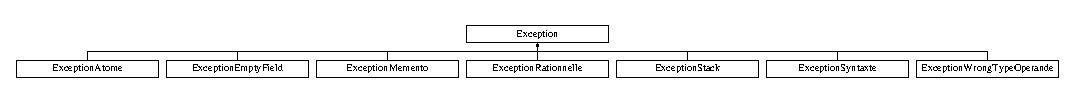
\includegraphics[height=0.812183cm]{class_exception}
\end{center}
\end{figure}
\subsection*{Public Member Functions}
\begin{DoxyCompactItemize}
\item 
\hyperlink{class_exception_a2f8585e6926cd25578104624cecab5c0}{Exception} (const Q\+String \&s)
\begin{DoxyCompactList}\small\item\em Contructeur. \end{DoxyCompactList}\item 
virtual \hyperlink{class_exception_ad1ba411de295ef2eeb02ba26284a829a}{$\sim$\+Exception} ()\hypertarget{class_exception_ad1ba411de295ef2eeb02ba26284a829a}{}\label{class_exception_ad1ba411de295ef2eeb02ba26284a829a}

\begin{DoxyCompactList}\small\item\em Destructeur d\textquotesingle{}une exception. \end{DoxyCompactList}\item 
virtual const Q\+String \& \hyperlink{class_exception_a73ce9dfab1e48800f8818978d014c106}{what} () const  =0
\begin{DoxyCompactList}\small\item\em Fonction virtuelle pure qui retourne le message de l\textquotesingle{}exception. \end{DoxyCompactList}\end{DoxyCompactItemize}
\subsection*{Protected Attributes}
\begin{DoxyCompactItemize}
\item 
Q\+String {\bfseries msg}\hypertarget{class_exception_a8f5843d9fdd54202dab2f2fb387ae71a}{}\label{class_exception_a8f5843d9fdd54202dab2f2fb387ae71a}

\end{DoxyCompactItemize}


\subsection{Detailed Description}
Classe mère abstraite pour gérer les exceptions. 

\subsection{Constructor \& Destructor Documentation}
\index{Exception@{Exception}!Exception@{Exception}}
\index{Exception@{Exception}!Exception@{Exception}}
\subsubsection[{\texorpdfstring{Exception(const Q\+String \&s)}{Exception(const QString &s)}}]{\setlength{\rightskip}{0pt plus 5cm}Exception\+::\+Exception (
\begin{DoxyParamCaption}
\item[{const Q\+String \&}]{s}
\end{DoxyParamCaption}
)\hspace{0.3cm}{\ttfamily [inline]}}\hypertarget{class_exception_a2f8585e6926cd25578104624cecab5c0}{}\label{class_exception_a2f8585e6926cd25578104624cecab5c0}


Contructeur. 


\begin{DoxyParams}{Parameters}
{\em s} & Message de l\textquotesingle{}exception \\
\hline
\end{DoxyParams}


\subsection{Member Function Documentation}
\index{Exception@{Exception}!what@{what}}
\index{what@{what}!Exception@{Exception}}
\subsubsection[{\texorpdfstring{what() const  =0}{what() const  =0}}]{\setlength{\rightskip}{0pt plus 5cm}virtual const Q\+String\& Exception\+::what (
\begin{DoxyParamCaption}
{}
\end{DoxyParamCaption}
) const\hspace{0.3cm}{\ttfamily [pure virtual]}}\hypertarget{class_exception_a73ce9dfab1e48800f8818978d014c106}{}\label{class_exception_a73ce9dfab1e48800f8818978d014c106}


Fonction virtuelle pure qui retourne le message de l\textquotesingle{}exception. 

\begin{DoxyReturn}{Returns}
Le texte de l\textquotesingle{}exception 
\end{DoxyReturn}


Implemented in \hyperlink{class_exception_empty_field_ac4d0d967d2651c5f79f9b94e8bd33be1}{Exception\+Empty\+Field}, \hyperlink{class_exception_syntaxte_a6bfbd6fe64c17610db8196c778e29758}{Exception\+Syntaxte}, \hyperlink{class_exception_atome_a7f44c61c6819f3bef675160fd201e4f2}{Exception\+Atome}, \hyperlink{class_exception_memento_a75c501d8bf4bd3bad2e3fb7bf17c778d}{Exception\+Memento}, \hyperlink{class_exception_wrong_type_operande_abf65a69fad540f7015838be5576fb55d}{Exception\+Wrong\+Type\+Operande}, \hyperlink{class_exception_rationnelle_a09a2ad10a9e9846a090fb0654dd12a05}{Exception\+Rationnelle}, and \hyperlink{class_exception_stack_a8e0dbc0a0c4077e5f1c873143e42d162}{Exception\+Stack}.



The documentation for this class was generated from the following file\+:\begin{DoxyCompactItemize}
\item 
exception.\+h\end{DoxyCompactItemize}

\hypertarget{class_exception_atome}{}\section{Exception\+Atome Class Reference}
\label{class_exception_atome}\index{Exception\+Atome@{Exception\+Atome}}


Classe d\textquotesingle{}exception pour les Litterales Atomes.  




{\ttfamily \#include $<$exception.\+h$>$}

Inheritance diagram for Exception\+Atome\+:\begin{figure}[H]
\begin{center}
\leavevmode
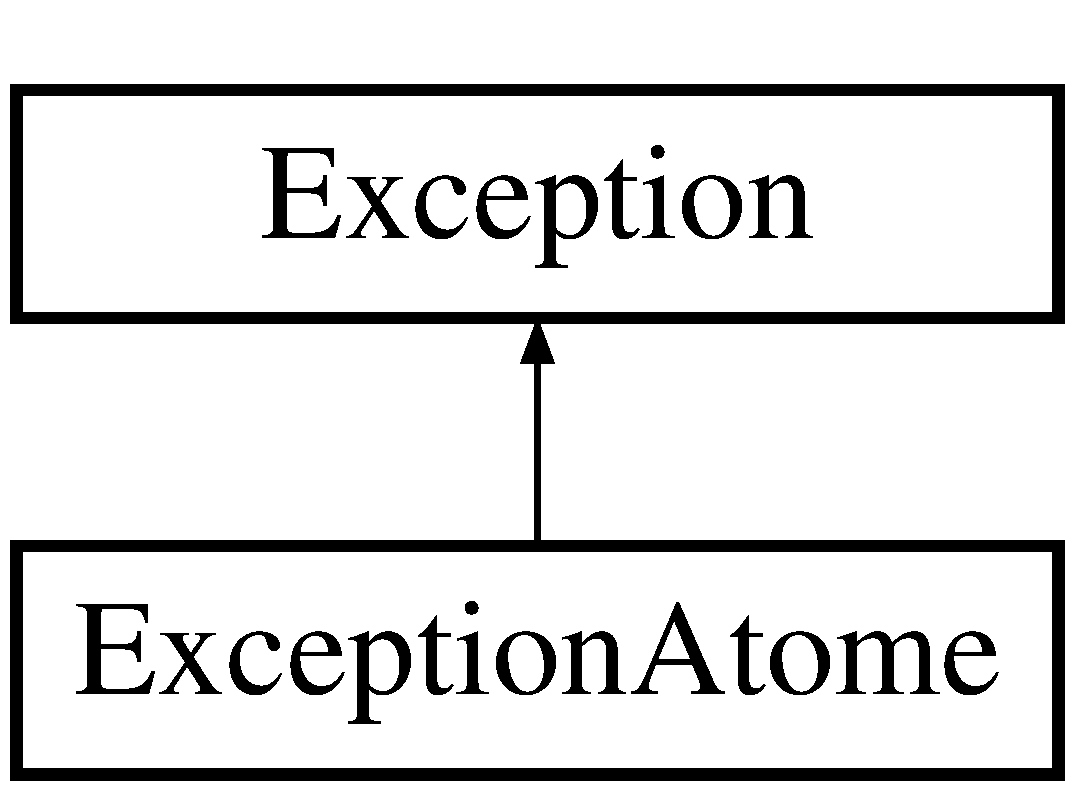
\includegraphics[height=2.000000cm]{class_exception_atome}
\end{center}
\end{figure}
\subsection*{Public Types}
\begin{DoxyCompactItemize}
\item 
enum \hyperlink{class_exception_atome_abb43c6c9a48f745dba9aaad0f721267d}{Type} \{ \hyperlink{class_exception_atome_abb43c6c9a48f745dba9aaad0f721267dafabbf1b0aaefd3fc099f9cecb11b1888}{A\+T\+O\+M\+E\+\_\+\+I\+S\+\_\+\+O\+P\+E\+R\+A\+T\+OR}
 \}\begin{DoxyCompactList}\small\item\em Type enum correspondant. \end{DoxyCompactList}
\end{DoxyCompactItemize}
\subsection*{Public Member Functions}
\begin{DoxyCompactItemize}
\item 
\hyperlink{class_exception_atome_a4facf977043886e2ea8539949d59a70f}{Exception\+Atome} (const \hyperlink{class_exception_atome_abb43c6c9a48f745dba9aaad0f721267d}{Type} t, const Q\+String \&s=\char`\"{}\char`\"{})
\begin{DoxyCompactList}\small\item\em Constructeur de l\textquotesingle{}exception. \end{DoxyCompactList}\item 
virtual \hyperlink{class_exception_atome_a6062e4843a817667c37a53014e31f81e}{$\sim$\+Exception\+Atome} ()\hypertarget{class_exception_atome_a6062e4843a817667c37a53014e31f81e}{}\label{class_exception_atome_a6062e4843a817667c37a53014e31f81e}

\begin{DoxyCompactList}\small\item\em Destructeur de l\textquotesingle{}exception. \end{DoxyCompactList}\item 
virtual const Q\+String \& \hyperlink{class_exception_atome_a7f44c61c6819f3bef675160fd201e4f2}{what} () const 
\begin{DoxyCompactList}\small\item\em Fonction qui retourne le message de l\textquotesingle{}exception. \end{DoxyCompactList}\item 
virtual \hyperlink{class_exception_atome_abb43c6c9a48f745dba9aaad0f721267d}{Type} \hyperlink{class_exception_atome_ac1756a673cf313054c118e6d3cccf843}{error\+Type} () const 
\begin{DoxyCompactList}\small\item\em Fonction qui retourne le type de l\textquotesingle{}exception. \end{DoxyCompactList}\end{DoxyCompactItemize}
\subsection*{Additional Inherited Members}


\subsection{Detailed Description}
Classe d\textquotesingle{}exception pour les Litterales Atomes. 

\subsection{Member Enumeration Documentation}
\index{Exception\+Atome@{Exception\+Atome}!Type@{Type}}
\index{Type@{Type}!Exception\+Atome@{Exception\+Atome}}
\subsubsection[{\texorpdfstring{Type}{Type}}]{\setlength{\rightskip}{0pt plus 5cm}enum {\bf Exception\+Atome\+::\+Type}}\hypertarget{class_exception_atome_abb43c6c9a48f745dba9aaad0f721267d}{}\label{class_exception_atome_abb43c6c9a48f745dba9aaad0f721267d}


Type enum correspondant. 

\begin{Desc}
\item[Enumerator]\par
\begin{description}
\index{A\+T\+O\+M\+E\+\_\+\+I\+S\+\_\+\+O\+P\+E\+R\+A\+T\+OR@{A\+T\+O\+M\+E\+\_\+\+I\+S\+\_\+\+O\+P\+E\+R\+A\+T\+OR}!Exception\+Atome@{Exception\+Atome}}\index{Exception\+Atome@{Exception\+Atome}!A\+T\+O\+M\+E\+\_\+\+I\+S\+\_\+\+O\+P\+E\+R\+A\+T\+OR@{A\+T\+O\+M\+E\+\_\+\+I\+S\+\_\+\+O\+P\+E\+R\+A\+T\+OR}}\item[{\em 
A\+T\+O\+M\+E\+\_\+\+I\+S\+\_\+\+O\+P\+E\+R\+A\+T\+OR\hypertarget{class_exception_atome_abb43c6c9a48f745dba9aaad0f721267dafabbf1b0aaefd3fc099f9cecb11b1888}{}\label{class_exception_atome_abb43c6c9a48f745dba9aaad0f721267dafabbf1b0aaefd3fc099f9cecb11b1888}
}]L\textquotesingle{}atome est déjà un opérateur connu \end{description}
\end{Desc}


\subsection{Constructor \& Destructor Documentation}
\index{Exception\+Atome@{Exception\+Atome}!Exception\+Atome@{Exception\+Atome}}
\index{Exception\+Atome@{Exception\+Atome}!Exception\+Atome@{Exception\+Atome}}
\subsubsection[{\texorpdfstring{Exception\+Atome(const Type t, const Q\+String \&s="""")}{ExceptionAtome(const Type t, const QString &s="")}}]{\setlength{\rightskip}{0pt plus 5cm}Exception\+Atome\+::\+Exception\+Atome (
\begin{DoxyParamCaption}
\item[{const {\bf Type}}]{t, }
\item[{const Q\+String \&}]{s = {\ttfamily \char`\"{}\char`\"{}}}
\end{DoxyParamCaption}
)\hspace{0.3cm}{\ttfamily [inline]}}\hypertarget{class_exception_atome_a4facf977043886e2ea8539949d59a70f}{}\label{class_exception_atome_a4facf977043886e2ea8539949d59a70f}


Constructeur de l\textquotesingle{}exception. 


\begin{DoxyParams}{Parameters}
{\em t} & Type de l\textquotesingle{}exception \\
\hline
{\em s} & Texte de l\textquotesingle{}exception \\
\hline
\end{DoxyParams}


\subsection{Member Function Documentation}
\index{Exception\+Atome@{Exception\+Atome}!error\+Type@{error\+Type}}
\index{error\+Type@{error\+Type}!Exception\+Atome@{Exception\+Atome}}
\subsubsection[{\texorpdfstring{error\+Type() const }{errorType() const }}]{\setlength{\rightskip}{0pt plus 5cm}virtual {\bf Type} Exception\+Atome\+::error\+Type (
\begin{DoxyParamCaption}
{}
\end{DoxyParamCaption}
) const\hspace{0.3cm}{\ttfamily [inline]}, {\ttfamily [virtual]}}\hypertarget{class_exception_atome_ac1756a673cf313054c118e6d3cccf843}{}\label{class_exception_atome_ac1756a673cf313054c118e6d3cccf843}


Fonction qui retourne le type de l\textquotesingle{}exception. 

\begin{DoxyReturn}{Returns}
Le type de l\textquotesingle{}exception 
\end{DoxyReturn}
\index{Exception\+Atome@{Exception\+Atome}!what@{what}}
\index{what@{what}!Exception\+Atome@{Exception\+Atome}}
\subsubsection[{\texorpdfstring{what() const }{what() const }}]{\setlength{\rightskip}{0pt plus 5cm}virtual const Q\+String\& Exception\+Atome\+::what (
\begin{DoxyParamCaption}
{}
\end{DoxyParamCaption}
) const\hspace{0.3cm}{\ttfamily [inline]}, {\ttfamily [virtual]}}\hypertarget{class_exception_atome_a7f44c61c6819f3bef675160fd201e4f2}{}\label{class_exception_atome_a7f44c61c6819f3bef675160fd201e4f2}


Fonction qui retourne le message de l\textquotesingle{}exception. 

\begin{DoxyReturn}{Returns}
Le texte de l\textquotesingle{}exception 
\end{DoxyReturn}


Implements \hyperlink{class_exception_a73ce9dfab1e48800f8818978d014c106}{Exception}.



The documentation for this class was generated from the following file\+:\begin{DoxyCompactItemize}
\item 
exception.\+h\end{DoxyCompactItemize}

\hypertarget{class_exception_empty_field}{}\section{Exception\+Empty\+Field Class Reference}
\label{class_exception_empty_field}\index{Exception\+Empty\+Field@{Exception\+Empty\+Field}}


Classe d\textquotesingle{}exception pour les vérifications des champs.  




{\ttfamily \#include $<$exception.\+h$>$}

Inheritance diagram for Exception\+Empty\+Field\+:\begin{figure}[H]
\begin{center}
\leavevmode
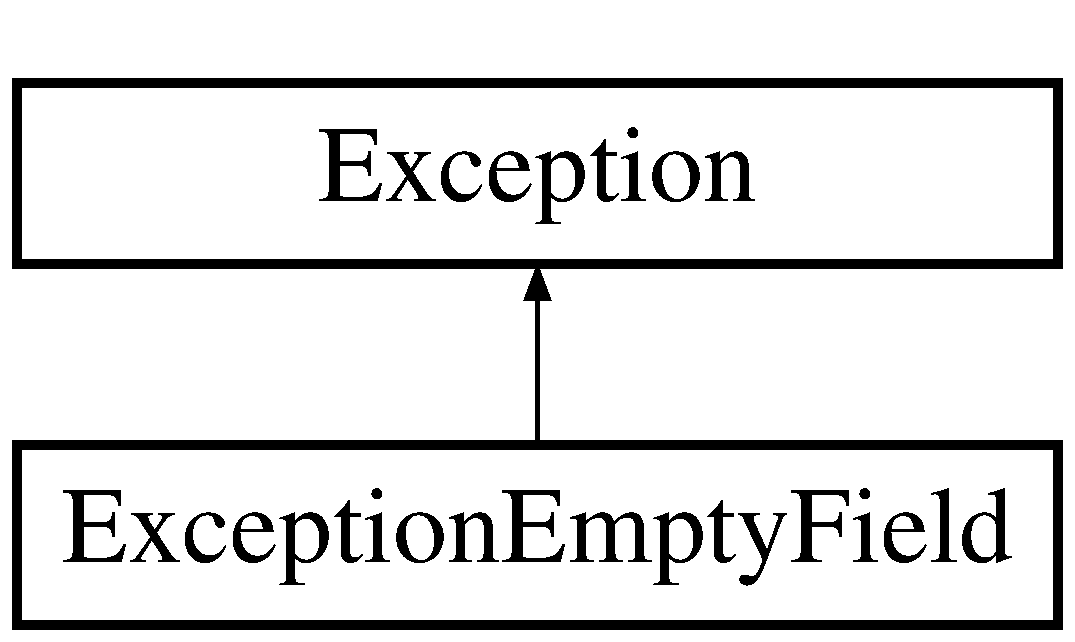
\includegraphics[height=2.000000cm]{class_exception_empty_field}
\end{center}
\end{figure}
\subsection*{Public Types}
\begin{DoxyCompactItemize}
\item 
enum \hyperlink{class_exception_empty_field_af667c68aa2b6c49ad147004ce9a09584}{Type} \{ \hyperlink{class_exception_empty_field_af667c68aa2b6c49ad147004ce9a09584a6bc8e6b4c1ce816868e981082235660f}{E\+M\+P\+T\+Y\+\_\+\+F\+I\+E\+LD}, 
\hyperlink{class_exception_empty_field_af667c68aa2b6c49ad147004ce9a09584a9b82c514a396c1eb0789ca58c037c273}{W\+R\+O\+N\+G\+\_\+\+N\+U\+M\+B\+E\+R\+\_\+\+S\+E\+L\+E\+C\+T\+ED}
 \}\begin{DoxyCompactList}\small\item\em Type enum correspondant. \end{DoxyCompactList}
\end{DoxyCompactItemize}
\subsection*{Public Member Functions}
\begin{DoxyCompactItemize}
\item 
\hyperlink{class_exception_empty_field_a66b400511c314e7bc5862fb86a879213}{Exception\+Empty\+Field} (const \hyperlink{class_exception_empty_field_af667c68aa2b6c49ad147004ce9a09584}{Type} t, const Q\+String \&s=\char`\"{}\char`\"{})
\begin{DoxyCompactList}\small\item\em Constructeur de l\textquotesingle{}exception. \end{DoxyCompactList}\item 
virtual \hyperlink{class_exception_empty_field_a47772f022b36af5b311e00f08cf2a58f}{$\sim$\+Exception\+Empty\+Field} ()\hypertarget{class_exception_empty_field_a47772f022b36af5b311e00f08cf2a58f}{}\label{class_exception_empty_field_a47772f022b36af5b311e00f08cf2a58f}

\begin{DoxyCompactList}\small\item\em Destructeur de l\textquotesingle{}exception. \end{DoxyCompactList}\item 
virtual const Q\+String \& \hyperlink{class_exception_empty_field_ac4d0d967d2651c5f79f9b94e8bd33be1}{what} () const 
\begin{DoxyCompactList}\small\item\em Fonction qui retourne le message de l\textquotesingle{}exception. \end{DoxyCompactList}\item 
virtual \hyperlink{class_exception_empty_field_af667c68aa2b6c49ad147004ce9a09584}{Type} \hyperlink{class_exception_empty_field_a4bb70e06dcd2a8631740245b58b5f6ec}{error\+Type} () const 
\begin{DoxyCompactList}\small\item\em Fonction qui retourne le type de l\textquotesingle{}exception. \end{DoxyCompactList}\end{DoxyCompactItemize}
\subsection*{Additional Inherited Members}


\subsection{Detailed Description}
Classe d\textquotesingle{}exception pour les vérifications des champs. 

\subsection{Member Enumeration Documentation}
\index{Exception\+Empty\+Field@{Exception\+Empty\+Field}!Type@{Type}}
\index{Type@{Type}!Exception\+Empty\+Field@{Exception\+Empty\+Field}}
\subsubsection[{\texorpdfstring{Type}{Type}}]{\setlength{\rightskip}{0pt plus 5cm}enum {\bf Exception\+Empty\+Field\+::\+Type}}\hypertarget{class_exception_empty_field_af667c68aa2b6c49ad147004ce9a09584}{}\label{class_exception_empty_field_af667c68aa2b6c49ad147004ce9a09584}


Type enum correspondant. 

\begin{Desc}
\item[Enumerator]\par
\begin{description}
\index{E\+M\+P\+T\+Y\+\_\+\+F\+I\+E\+LD@{E\+M\+P\+T\+Y\+\_\+\+F\+I\+E\+LD}!Exception\+Empty\+Field@{Exception\+Empty\+Field}}\index{Exception\+Empty\+Field@{Exception\+Empty\+Field}!E\+M\+P\+T\+Y\+\_\+\+F\+I\+E\+LD@{E\+M\+P\+T\+Y\+\_\+\+F\+I\+E\+LD}}\item[{\em 
E\+M\+P\+T\+Y\+\_\+\+F\+I\+E\+LD\hypertarget{class_exception_empty_field_af667c68aa2b6c49ad147004ce9a09584a6bc8e6b4c1ce816868e981082235660f}{}\label{class_exception_empty_field_af667c68aa2b6c49ad147004ce9a09584a6bc8e6b4c1ce816868e981082235660f}
}]Le champs de texte est vide \index{W\+R\+O\+N\+G\+\_\+\+N\+U\+M\+B\+E\+R\+\_\+\+S\+E\+L\+E\+C\+T\+ED@{W\+R\+O\+N\+G\+\_\+\+N\+U\+M\+B\+E\+R\+\_\+\+S\+E\+L\+E\+C\+T\+ED}!Exception\+Empty\+Field@{Exception\+Empty\+Field}}\index{Exception\+Empty\+Field@{Exception\+Empty\+Field}!W\+R\+O\+N\+G\+\_\+\+N\+U\+M\+B\+E\+R\+\_\+\+S\+E\+L\+E\+C\+T\+ED@{W\+R\+O\+N\+G\+\_\+\+N\+U\+M\+B\+E\+R\+\_\+\+S\+E\+L\+E\+C\+T\+ED}}\item[{\em 
W\+R\+O\+N\+G\+\_\+\+N\+U\+M\+B\+E\+R\+\_\+\+S\+E\+L\+E\+C\+T\+ED\hypertarget{class_exception_empty_field_af667c68aa2b6c49ad147004ce9a09584a9b82c514a396c1eb0789ca58c037c273}{}\label{class_exception_empty_field_af667c68aa2b6c49ad147004ce9a09584a9b82c514a396c1eb0789ca58c037c273}
}]Le nombre de champs sélectionné est incorrect \end{description}
\end{Desc}


\subsection{Constructor \& Destructor Documentation}
\index{Exception\+Empty\+Field@{Exception\+Empty\+Field}!Exception\+Empty\+Field@{Exception\+Empty\+Field}}
\index{Exception\+Empty\+Field@{Exception\+Empty\+Field}!Exception\+Empty\+Field@{Exception\+Empty\+Field}}
\subsubsection[{\texorpdfstring{Exception\+Empty\+Field(const Type t, const Q\+String \&s="""")}{ExceptionEmptyField(const Type t, const QString &s="")}}]{\setlength{\rightskip}{0pt plus 5cm}Exception\+Empty\+Field\+::\+Exception\+Empty\+Field (
\begin{DoxyParamCaption}
\item[{const {\bf Type}}]{t, }
\item[{const Q\+String \&}]{s = {\ttfamily \char`\"{}\char`\"{}}}
\end{DoxyParamCaption}
)\hspace{0.3cm}{\ttfamily [inline]}}\hypertarget{class_exception_empty_field_a66b400511c314e7bc5862fb86a879213}{}\label{class_exception_empty_field_a66b400511c314e7bc5862fb86a879213}


Constructeur de l\textquotesingle{}exception. 


\begin{DoxyParams}{Parameters}
{\em t} & Type de l\textquotesingle{}exception \\
\hline
{\em s} & Texte de l\textquotesingle{}exception \\
\hline
\end{DoxyParams}


\subsection{Member Function Documentation}
\index{Exception\+Empty\+Field@{Exception\+Empty\+Field}!error\+Type@{error\+Type}}
\index{error\+Type@{error\+Type}!Exception\+Empty\+Field@{Exception\+Empty\+Field}}
\subsubsection[{\texorpdfstring{error\+Type() const }{errorType() const }}]{\setlength{\rightskip}{0pt plus 5cm}virtual {\bf Type} Exception\+Empty\+Field\+::error\+Type (
\begin{DoxyParamCaption}
{}
\end{DoxyParamCaption}
) const\hspace{0.3cm}{\ttfamily [inline]}, {\ttfamily [virtual]}}\hypertarget{class_exception_empty_field_a4bb70e06dcd2a8631740245b58b5f6ec}{}\label{class_exception_empty_field_a4bb70e06dcd2a8631740245b58b5f6ec}


Fonction qui retourne le type de l\textquotesingle{}exception. 

\begin{DoxyReturn}{Returns}
Le type de l\textquotesingle{}exception 
\end{DoxyReturn}
\index{Exception\+Empty\+Field@{Exception\+Empty\+Field}!what@{what}}
\index{what@{what}!Exception\+Empty\+Field@{Exception\+Empty\+Field}}
\subsubsection[{\texorpdfstring{what() const }{what() const }}]{\setlength{\rightskip}{0pt plus 5cm}virtual const Q\+String\& Exception\+Empty\+Field\+::what (
\begin{DoxyParamCaption}
{}
\end{DoxyParamCaption}
) const\hspace{0.3cm}{\ttfamily [inline]}, {\ttfamily [virtual]}}\hypertarget{class_exception_empty_field_ac4d0d967d2651c5f79f9b94e8bd33be1}{}\label{class_exception_empty_field_ac4d0d967d2651c5f79f9b94e8bd33be1}


Fonction qui retourne le message de l\textquotesingle{}exception. 

\begin{DoxyReturn}{Returns}
Le texte de l\textquotesingle{}exception 
\end{DoxyReturn}


Implements \hyperlink{class_exception_a73ce9dfab1e48800f8818978d014c106}{Exception}.



The documentation for this class was generated from the following file\+:\begin{DoxyCompactItemize}
\item 
exception.\+h\end{DoxyCompactItemize}

\hypertarget{class_exception_memento}{}\section{Exception\+Memento Class Reference}
\label{class_exception_memento}\index{Exception\+Memento@{Exception\+Memento}}


Classe d\textquotesingle{}exception pour le design pattern \hyperlink{class_memento}{Memento} et la gestion de l\textquotesingle{}Undo Redo.  




{\ttfamily \#include $<$exception.\+h$>$}

Inheritance diagram for Exception\+Memento\+:\begin{figure}[H]
\begin{center}
\leavevmode
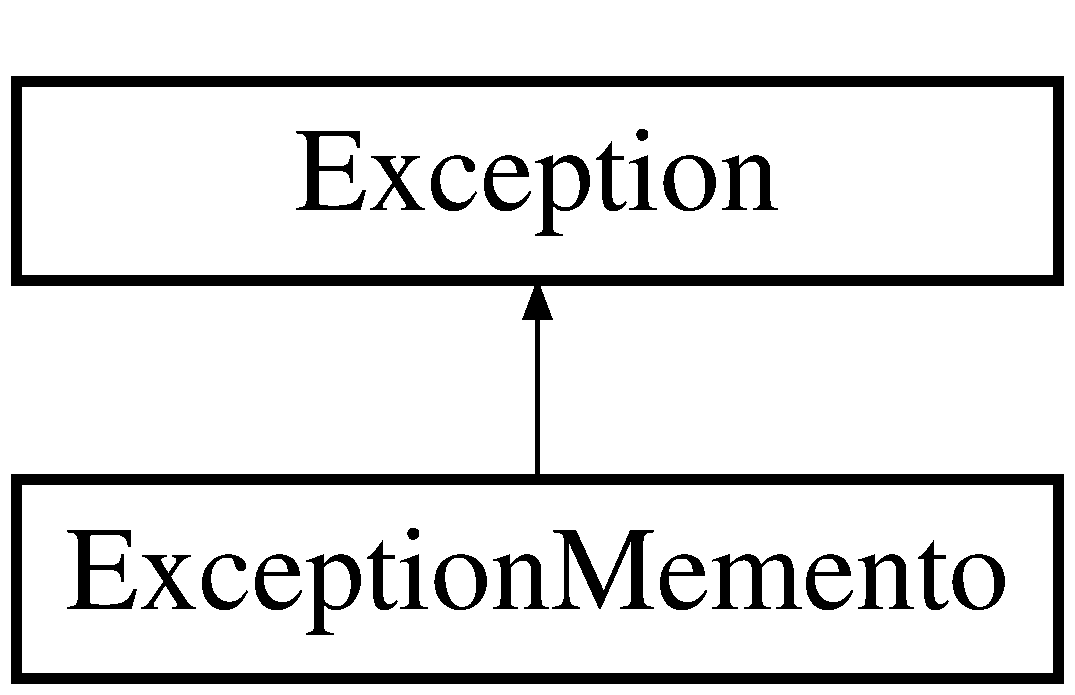
\includegraphics[height=2.000000cm]{class_exception_memento}
\end{center}
\end{figure}
\subsection*{Public Types}
\begin{DoxyCompactItemize}
\item 
enum \hyperlink{class_exception_memento_a83ec20464c7ba61569afeb4477f1504e}{Type} \{ \hyperlink{class_exception_memento_a83ec20464c7ba61569afeb4477f1504ea9f16db6c0e64e2a901a245fdf853058a}{C\+A\+N\+N\+O\+T\+\_\+\+U\+N\+DO}, 
\hyperlink{class_exception_memento_a83ec20464c7ba61569afeb4477f1504eae5de90f573b1df7d52ef3c32bf80f4b5}{C\+A\+N\+N\+O\+T\+\_\+\+R\+E\+DO}
 \}\begin{DoxyCompactList}\small\item\em Type enum correspondant. \end{DoxyCompactList}
\end{DoxyCompactItemize}
\subsection*{Public Member Functions}
\begin{DoxyCompactItemize}
\item 
\hyperlink{class_exception_memento_a1e94b6bb22c1b90247a40729d7ac3271}{Exception\+Memento} (const \hyperlink{class_exception_memento_a83ec20464c7ba61569afeb4477f1504e}{Type} t, const Q\+String \&s=\char`\"{}\char`\"{})
\begin{DoxyCompactList}\small\item\em Constructeur de l\textquotesingle{}exception. \end{DoxyCompactList}\item 
virtual \hyperlink{class_exception_memento_ac3f0964c8f4ac3c1ac7fa58a96ade038}{$\sim$\+Exception\+Memento} ()\hypertarget{class_exception_memento_ac3f0964c8f4ac3c1ac7fa58a96ade038}{}\label{class_exception_memento_ac3f0964c8f4ac3c1ac7fa58a96ade038}

\begin{DoxyCompactList}\small\item\em Destructeur de l\textquotesingle{}exception. \end{DoxyCompactList}\item 
virtual const Q\+String \& \hyperlink{class_exception_memento_a75c501d8bf4bd3bad2e3fb7bf17c778d}{what} () const 
\begin{DoxyCompactList}\small\item\em Fonction qui retourne le message de l\textquotesingle{}exception. \end{DoxyCompactList}\item 
virtual \hyperlink{class_exception_memento_a83ec20464c7ba61569afeb4477f1504e}{Type} \hyperlink{class_exception_memento_a1a09d1650a93d2b54fd2e167a6968b1b}{error\+Type} () const 
\begin{DoxyCompactList}\small\item\em Fonction qui retourne le type de l\textquotesingle{}exception. \end{DoxyCompactList}\end{DoxyCompactItemize}
\subsection*{Additional Inherited Members}


\subsection{Detailed Description}
Classe d\textquotesingle{}exception pour le design pattern \hyperlink{class_memento}{Memento} et la gestion de l\textquotesingle{}Undo Redo. 

\subsection{Member Enumeration Documentation}
\index{Exception\+Memento@{Exception\+Memento}!Type@{Type}}
\index{Type@{Type}!Exception\+Memento@{Exception\+Memento}}
\subsubsection[{\texorpdfstring{Type}{Type}}]{\setlength{\rightskip}{0pt plus 5cm}enum {\bf Exception\+Memento\+::\+Type}}\hypertarget{class_exception_memento_a83ec20464c7ba61569afeb4477f1504e}{}\label{class_exception_memento_a83ec20464c7ba61569afeb4477f1504e}


Type enum correspondant. 

\begin{Desc}
\item[Enumerator]\par
\begin{description}
\index{C\+A\+N\+N\+O\+T\+\_\+\+U\+N\+DO@{C\+A\+N\+N\+O\+T\+\_\+\+U\+N\+DO}!Exception\+Memento@{Exception\+Memento}}\index{Exception\+Memento@{Exception\+Memento}!C\+A\+N\+N\+O\+T\+\_\+\+U\+N\+DO@{C\+A\+N\+N\+O\+T\+\_\+\+U\+N\+DO}}\item[{\em 
C\+A\+N\+N\+O\+T\+\_\+\+U\+N\+DO\hypertarget{class_exception_memento_a83ec20464c7ba61569afeb4477f1504ea9f16db6c0e64e2a901a245fdf853058a}{}\label{class_exception_memento_a83ec20464c7ba61569afeb4477f1504ea9f16db6c0e64e2a901a245fdf853058a}
}]Impossible de revenir à l\textquotesingle{}état précédent \index{C\+A\+N\+N\+O\+T\+\_\+\+R\+E\+DO@{C\+A\+N\+N\+O\+T\+\_\+\+R\+E\+DO}!Exception\+Memento@{Exception\+Memento}}\index{Exception\+Memento@{Exception\+Memento}!C\+A\+N\+N\+O\+T\+\_\+\+R\+E\+DO@{C\+A\+N\+N\+O\+T\+\_\+\+R\+E\+DO}}\item[{\em 
C\+A\+N\+N\+O\+T\+\_\+\+R\+E\+DO\hypertarget{class_exception_memento_a83ec20464c7ba61569afeb4477f1504eae5de90f573b1df7d52ef3c32bf80f4b5}{}\label{class_exception_memento_a83ec20464c7ba61569afeb4477f1504eae5de90f573b1df7d52ef3c32bf80f4b5}
}]Impossible de revenir à l\textquotesingle{}état suivant \end{description}
\end{Desc}


\subsection{Constructor \& Destructor Documentation}
\index{Exception\+Memento@{Exception\+Memento}!Exception\+Memento@{Exception\+Memento}}
\index{Exception\+Memento@{Exception\+Memento}!Exception\+Memento@{Exception\+Memento}}
\subsubsection[{\texorpdfstring{Exception\+Memento(const Type t, const Q\+String \&s="""")}{ExceptionMemento(const Type t, const QString &s="")}}]{\setlength{\rightskip}{0pt plus 5cm}Exception\+Memento\+::\+Exception\+Memento (
\begin{DoxyParamCaption}
\item[{const {\bf Type}}]{t, }
\item[{const Q\+String \&}]{s = {\ttfamily \char`\"{}\char`\"{}}}
\end{DoxyParamCaption}
)\hspace{0.3cm}{\ttfamily [inline]}}\hypertarget{class_exception_memento_a1e94b6bb22c1b90247a40729d7ac3271}{}\label{class_exception_memento_a1e94b6bb22c1b90247a40729d7ac3271}


Constructeur de l\textquotesingle{}exception. 


\begin{DoxyParams}{Parameters}
{\em t} & Type de l\textquotesingle{}exception \\
\hline
{\em s} & Texte de l\textquotesingle{}exception \\
\hline
\end{DoxyParams}


\subsection{Member Function Documentation}
\index{Exception\+Memento@{Exception\+Memento}!error\+Type@{error\+Type}}
\index{error\+Type@{error\+Type}!Exception\+Memento@{Exception\+Memento}}
\subsubsection[{\texorpdfstring{error\+Type() const }{errorType() const }}]{\setlength{\rightskip}{0pt plus 5cm}virtual {\bf Type} Exception\+Memento\+::error\+Type (
\begin{DoxyParamCaption}
{}
\end{DoxyParamCaption}
) const\hspace{0.3cm}{\ttfamily [inline]}, {\ttfamily [virtual]}}\hypertarget{class_exception_memento_a1a09d1650a93d2b54fd2e167a6968b1b}{}\label{class_exception_memento_a1a09d1650a93d2b54fd2e167a6968b1b}


Fonction qui retourne le type de l\textquotesingle{}exception. 

\begin{DoxyReturn}{Returns}
Le type de l\textquotesingle{}exception 
\end{DoxyReturn}
\index{Exception\+Memento@{Exception\+Memento}!what@{what}}
\index{what@{what}!Exception\+Memento@{Exception\+Memento}}
\subsubsection[{\texorpdfstring{what() const }{what() const }}]{\setlength{\rightskip}{0pt plus 5cm}virtual const Q\+String\& Exception\+Memento\+::what (
\begin{DoxyParamCaption}
{}
\end{DoxyParamCaption}
) const\hspace{0.3cm}{\ttfamily [inline]}, {\ttfamily [virtual]}}\hypertarget{class_exception_memento_a75c501d8bf4bd3bad2e3fb7bf17c778d}{}\label{class_exception_memento_a75c501d8bf4bd3bad2e3fb7bf17c778d}


Fonction qui retourne le message de l\textquotesingle{}exception. 

\begin{DoxyReturn}{Returns}
Le texte de l\textquotesingle{}exception 
\end{DoxyReturn}


Implements \hyperlink{class_exception_a73ce9dfab1e48800f8818978d014c106}{Exception}.



The documentation for this class was generated from the following file\+:\begin{DoxyCompactItemize}
\item 
exception.\+h\end{DoxyCompactItemize}

\hypertarget{class_exception_rationnelle}{}\section{Exception\+Rationnelle Class Reference}
\label{class_exception_rationnelle}\index{Exception\+Rationnelle@{Exception\+Rationnelle}}


Classe d\textquotesingle{}exception pour les Litterales Rationnelles.  




{\ttfamily \#include $<$exception.\+h$>$}

Inheritance diagram for Exception\+Rationnelle\+:\begin{figure}[H]
\begin{center}
\leavevmode
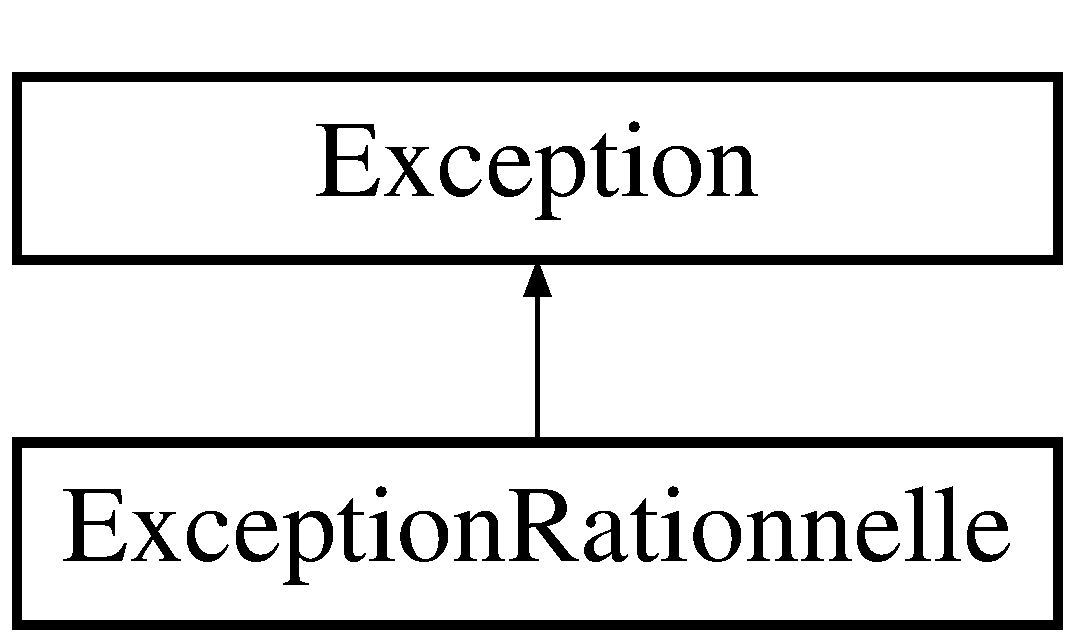
\includegraphics[height=2.000000cm]{class_exception_rationnelle}
\end{center}
\end{figure}
\subsection*{Public Types}
\begin{DoxyCompactItemize}
\item 
enum \hyperlink{class_exception_rationnelle_ac394933986da15ec9b40db3d46c32887}{Type} \{ \hyperlink{class_exception_rationnelle_ac394933986da15ec9b40db3d46c32887ae3c5fa15bcea676f55a4fcce0ae51a91}{C\+A\+N\+N\+O\+T\+\_\+\+H\+A\+V\+E\+\_\+\+D\+E\+N\+U\+M\+\_\+\+Z\+E\+RO}, 
\hyperlink{class_exception_rationnelle_ac394933986da15ec9b40db3d46c32887a31e2f21aee48d4ad850974bcfc7530a3}{U\+N\+K\+N\+O\+W\+N\+\_\+\+S\+E\+P\+A\+R\+A\+T\+OR}
 \}\begin{DoxyCompactList}\small\item\em Type enum correspondant. \end{DoxyCompactList}
\end{DoxyCompactItemize}
\subsection*{Public Member Functions}
\begin{DoxyCompactItemize}
\item 
\hyperlink{class_exception_rationnelle_af513b6155626b0582b700f366b19868f}{Exception\+Rationnelle} (const \hyperlink{class_exception_rationnelle_ac394933986da15ec9b40db3d46c32887}{Type} t, const Q\+String \&s=\char`\"{}\char`\"{})
\begin{DoxyCompactList}\small\item\em Constructeur de l\textquotesingle{}exception. \end{DoxyCompactList}\item 
virtual \hyperlink{class_exception_rationnelle_ae606e24017d4b5accf5878b6fee5be6c}{$\sim$\+Exception\+Rationnelle} ()\hypertarget{class_exception_rationnelle_ae606e24017d4b5accf5878b6fee5be6c}{}\label{class_exception_rationnelle_ae606e24017d4b5accf5878b6fee5be6c}

\begin{DoxyCompactList}\small\item\em Destructeur de l\textquotesingle{}exception. \end{DoxyCompactList}\item 
virtual const Q\+String \& \hyperlink{class_exception_rationnelle_a09a2ad10a9e9846a090fb0654dd12a05}{what} () const 
\begin{DoxyCompactList}\small\item\em Fonction qui retourne le message de l\textquotesingle{}exception. \end{DoxyCompactList}\item 
virtual \hyperlink{class_exception_rationnelle_ac394933986da15ec9b40db3d46c32887}{Type} \hyperlink{class_exception_rationnelle_a5b49afaeb0dba99688c25466d57df586}{error\+Type} () const 
\begin{DoxyCompactList}\small\item\em Fonction qui retourne le type de l\textquotesingle{}exception. \end{DoxyCompactList}\end{DoxyCompactItemize}
\subsection*{Additional Inherited Members}


\subsection{Detailed Description}
Classe d\textquotesingle{}exception pour les Litterales Rationnelles. 

\subsection{Member Enumeration Documentation}
\index{Exception\+Rationnelle@{Exception\+Rationnelle}!Type@{Type}}
\index{Type@{Type}!Exception\+Rationnelle@{Exception\+Rationnelle}}
\subsubsection[{\texorpdfstring{Type}{Type}}]{\setlength{\rightskip}{0pt plus 5cm}enum {\bf Exception\+Rationnelle\+::\+Type}}\hypertarget{class_exception_rationnelle_ac394933986da15ec9b40db3d46c32887}{}\label{class_exception_rationnelle_ac394933986da15ec9b40db3d46c32887}


Type enum correspondant. 

\begin{Desc}
\item[Enumerator]\par
\begin{description}
\index{C\+A\+N\+N\+O\+T\+\_\+\+H\+A\+V\+E\+\_\+\+D\+E\+N\+U\+M\+\_\+\+Z\+E\+RO@{C\+A\+N\+N\+O\+T\+\_\+\+H\+A\+V\+E\+\_\+\+D\+E\+N\+U\+M\+\_\+\+Z\+E\+RO}!Exception\+Rationnelle@{Exception\+Rationnelle}}\index{Exception\+Rationnelle@{Exception\+Rationnelle}!C\+A\+N\+N\+O\+T\+\_\+\+H\+A\+V\+E\+\_\+\+D\+E\+N\+U\+M\+\_\+\+Z\+E\+RO@{C\+A\+N\+N\+O\+T\+\_\+\+H\+A\+V\+E\+\_\+\+D\+E\+N\+U\+M\+\_\+\+Z\+E\+RO}}\item[{\em 
C\+A\+N\+N\+O\+T\+\_\+\+H\+A\+V\+E\+\_\+\+D\+E\+N\+U\+M\+\_\+\+Z\+E\+RO\hypertarget{class_exception_rationnelle_ac394933986da15ec9b40db3d46c32887ae3c5fa15bcea676f55a4fcce0ae51a91}{}\label{class_exception_rationnelle_ac394933986da15ec9b40db3d46c32887ae3c5fa15bcea676f55a4fcce0ae51a91}
}]Si le dénominateur vaut 0 \index{U\+N\+K\+N\+O\+W\+N\+\_\+\+S\+E\+P\+A\+R\+A\+T\+OR@{U\+N\+K\+N\+O\+W\+N\+\_\+\+S\+E\+P\+A\+R\+A\+T\+OR}!Exception\+Rationnelle@{Exception\+Rationnelle}}\index{Exception\+Rationnelle@{Exception\+Rationnelle}!U\+N\+K\+N\+O\+W\+N\+\_\+\+S\+E\+P\+A\+R\+A\+T\+OR@{U\+N\+K\+N\+O\+W\+N\+\_\+\+S\+E\+P\+A\+R\+A\+T\+OR}}\item[{\em 
U\+N\+K\+N\+O\+W\+N\+\_\+\+S\+E\+P\+A\+R\+A\+T\+OR\hypertarget{class_exception_rationnelle_ac394933986da15ec9b40db3d46c32887a31e2f21aee48d4ad850974bcfc7530a3}{}\label{class_exception_rationnelle_ac394933986da15ec9b40db3d46c32887a31e2f21aee48d4ad850974bcfc7530a3}
}]Si le séparateur est inconnu \end{description}
\end{Desc}


\subsection{Constructor \& Destructor Documentation}
\index{Exception\+Rationnelle@{Exception\+Rationnelle}!Exception\+Rationnelle@{Exception\+Rationnelle}}
\index{Exception\+Rationnelle@{Exception\+Rationnelle}!Exception\+Rationnelle@{Exception\+Rationnelle}}
\subsubsection[{\texorpdfstring{Exception\+Rationnelle(const Type t, const Q\+String \&s="""")}{ExceptionRationnelle(const Type t, const QString &s="")}}]{\setlength{\rightskip}{0pt plus 5cm}Exception\+Rationnelle\+::\+Exception\+Rationnelle (
\begin{DoxyParamCaption}
\item[{const {\bf Type}}]{t, }
\item[{const Q\+String \&}]{s = {\ttfamily \char`\"{}\char`\"{}}}
\end{DoxyParamCaption}
)\hspace{0.3cm}{\ttfamily [inline]}}\hypertarget{class_exception_rationnelle_af513b6155626b0582b700f366b19868f}{}\label{class_exception_rationnelle_af513b6155626b0582b700f366b19868f}


Constructeur de l\textquotesingle{}exception. 


\begin{DoxyParams}{Parameters}
{\em t} & Type de l\textquotesingle{}exception \\
\hline
{\em s} & Texte de l\textquotesingle{}exception \\
\hline
\end{DoxyParams}


\subsection{Member Function Documentation}
\index{Exception\+Rationnelle@{Exception\+Rationnelle}!error\+Type@{error\+Type}}
\index{error\+Type@{error\+Type}!Exception\+Rationnelle@{Exception\+Rationnelle}}
\subsubsection[{\texorpdfstring{error\+Type() const }{errorType() const }}]{\setlength{\rightskip}{0pt plus 5cm}virtual {\bf Type} Exception\+Rationnelle\+::error\+Type (
\begin{DoxyParamCaption}
{}
\end{DoxyParamCaption}
) const\hspace{0.3cm}{\ttfamily [inline]}, {\ttfamily [virtual]}}\hypertarget{class_exception_rationnelle_a5b49afaeb0dba99688c25466d57df586}{}\label{class_exception_rationnelle_a5b49afaeb0dba99688c25466d57df586}


Fonction qui retourne le type de l\textquotesingle{}exception. 

\begin{DoxyReturn}{Returns}
Le type de l\textquotesingle{}exception 
\end{DoxyReturn}
\index{Exception\+Rationnelle@{Exception\+Rationnelle}!what@{what}}
\index{what@{what}!Exception\+Rationnelle@{Exception\+Rationnelle}}
\subsubsection[{\texorpdfstring{what() const }{what() const }}]{\setlength{\rightskip}{0pt plus 5cm}virtual const Q\+String\& Exception\+Rationnelle\+::what (
\begin{DoxyParamCaption}
{}
\end{DoxyParamCaption}
) const\hspace{0.3cm}{\ttfamily [inline]}, {\ttfamily [virtual]}}\hypertarget{class_exception_rationnelle_a09a2ad10a9e9846a090fb0654dd12a05}{}\label{class_exception_rationnelle_a09a2ad10a9e9846a090fb0654dd12a05}


Fonction qui retourne le message de l\textquotesingle{}exception. 

\begin{DoxyReturn}{Returns}
Le texte de l\textquotesingle{}exception 
\end{DoxyReturn}


Implements \hyperlink{class_exception_a73ce9dfab1e48800f8818978d014c106}{Exception}.



The documentation for this class was generated from the following file\+:\begin{DoxyCompactItemize}
\item 
exception.\+h\end{DoxyCompactItemize}

\hypertarget{class_exception_stack}{}\section{Exception\+Stack Class Reference}
\label{class_exception_stack}\index{Exception\+Stack@{Exception\+Stack}}


Classe d\textquotesingle{}exception de la pile.  




{\ttfamily \#include $<$exception.\+h$>$}

Inheritance diagram for Exception\+Stack\+:\begin{figure}[H]
\begin{center}
\leavevmode
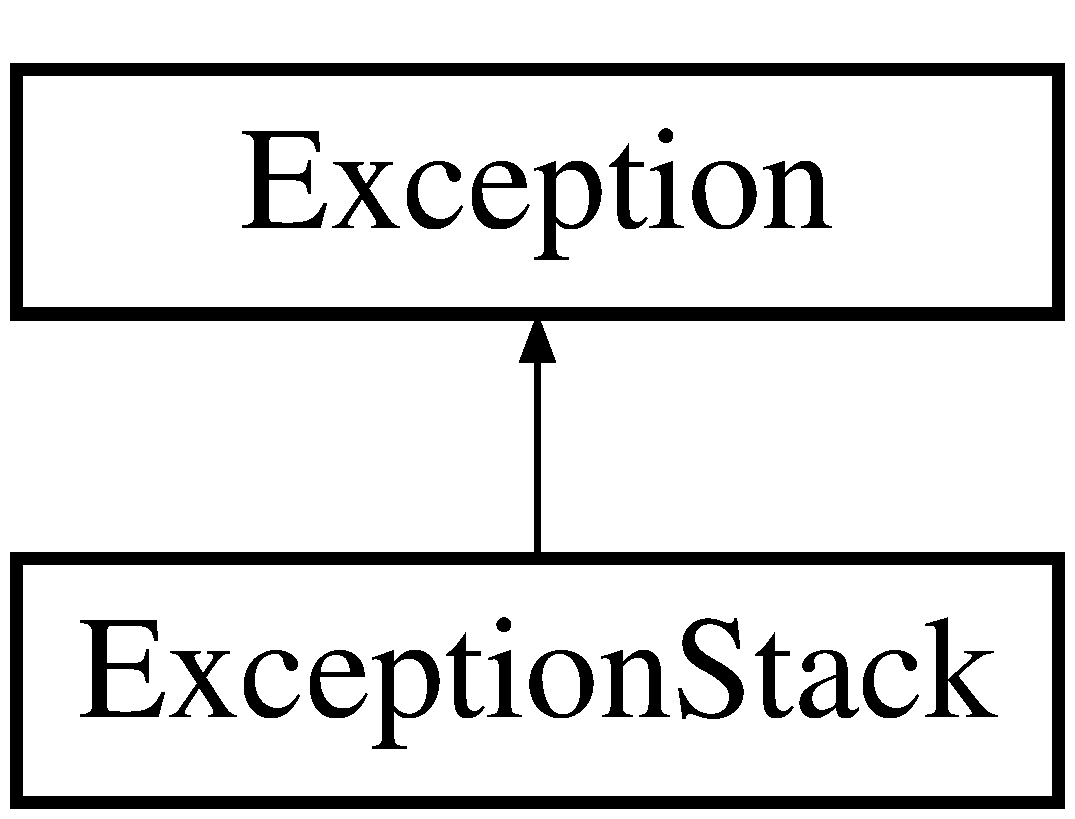
\includegraphics[height=2.000000cm]{class_exception_stack}
\end{center}
\end{figure}
\subsection*{Public Types}
\begin{DoxyCompactItemize}
\item 
enum \hyperlink{class_exception_stack_a79d7356c90bf8e48387a32723e7fe298}{Type} \{ \hyperlink{class_exception_stack_a79d7356c90bf8e48387a32723e7fe298a44e3e60c8f4046deae4da88e3d02493f}{C\+A\+N\+N\+O\+T\+\_\+\+P\+O\+P\+\_\+\+S\+T\+A\+C\+K\+\_\+\+E\+M\+P\+TY}
 \}\begin{DoxyCompactList}\small\item\em Type enum correspondant. \end{DoxyCompactList}
\end{DoxyCompactItemize}
\subsection*{Public Member Functions}
\begin{DoxyCompactItemize}
\item 
\hyperlink{class_exception_stack_a3dbb55d821b2b7a6071fbdab8691d624}{Exception\+Stack} (const \hyperlink{class_exception_stack_a79d7356c90bf8e48387a32723e7fe298}{Type} t, const Q\+String \&s=\char`\"{}\char`\"{})
\begin{DoxyCompactList}\small\item\em Constructeur de l\textquotesingle{}exception. \end{DoxyCompactList}\item 
virtual \hyperlink{class_exception_stack_a88cafb1273ee7b0ba1150ec03760cf26}{$\sim$\+Exception\+Stack} ()\hypertarget{class_exception_stack_a88cafb1273ee7b0ba1150ec03760cf26}{}\label{class_exception_stack_a88cafb1273ee7b0ba1150ec03760cf26}

\begin{DoxyCompactList}\small\item\em Destructeur de l\textquotesingle{}exception. \end{DoxyCompactList}\item 
virtual const Q\+String \& \hyperlink{class_exception_stack_a8e0dbc0a0c4077e5f1c873143e42d162}{what} () const 
\begin{DoxyCompactList}\small\item\em Fonction qui retourne le message de l\textquotesingle{}exception. \end{DoxyCompactList}\item 
virtual \hyperlink{class_exception_stack_a79d7356c90bf8e48387a32723e7fe298}{Type} \hyperlink{class_exception_stack_ac59bf40720ddb0a43d368d5bd94cbebc}{error\+Type} () const 
\begin{DoxyCompactList}\small\item\em Fonction qui retourne le type de l\textquotesingle{}exception. \end{DoxyCompactList}\end{DoxyCompactItemize}
\subsection*{Additional Inherited Members}


\subsection{Detailed Description}
Classe d\textquotesingle{}exception de la pile. 

\subsection{Member Enumeration Documentation}
\index{Exception\+Stack@{Exception\+Stack}!Type@{Type}}
\index{Type@{Type}!Exception\+Stack@{Exception\+Stack}}
\subsubsection[{\texorpdfstring{Type}{Type}}]{\setlength{\rightskip}{0pt plus 5cm}enum {\bf Exception\+Stack\+::\+Type}}\hypertarget{class_exception_stack_a79d7356c90bf8e48387a32723e7fe298}{}\label{class_exception_stack_a79d7356c90bf8e48387a32723e7fe298}


Type enum correspondant. 

\begin{Desc}
\item[Enumerator]\par
\begin{description}
\index{C\+A\+N\+N\+O\+T\+\_\+\+P\+O\+P\+\_\+\+S\+T\+A\+C\+K\+\_\+\+E\+M\+P\+TY@{C\+A\+N\+N\+O\+T\+\_\+\+P\+O\+P\+\_\+\+S\+T\+A\+C\+K\+\_\+\+E\+M\+P\+TY}!Exception\+Stack@{Exception\+Stack}}\index{Exception\+Stack@{Exception\+Stack}!C\+A\+N\+N\+O\+T\+\_\+\+P\+O\+P\+\_\+\+S\+T\+A\+C\+K\+\_\+\+E\+M\+P\+TY@{C\+A\+N\+N\+O\+T\+\_\+\+P\+O\+P\+\_\+\+S\+T\+A\+C\+K\+\_\+\+E\+M\+P\+TY}}\item[{\em 
C\+A\+N\+N\+O\+T\+\_\+\+P\+O\+P\+\_\+\+S\+T\+A\+C\+K\+\_\+\+E\+M\+P\+TY\hypertarget{class_exception_stack_a79d7356c90bf8e48387a32723e7fe298a44e3e60c8f4046deae4da88e3d02493f}{}\label{class_exception_stack_a79d7356c90bf8e48387a32723e7fe298a44e3e60c8f4046deae4da88e3d02493f}
}]Si la pile est vide \end{description}
\end{Desc}


\subsection{Constructor \& Destructor Documentation}
\index{Exception\+Stack@{Exception\+Stack}!Exception\+Stack@{Exception\+Stack}}
\index{Exception\+Stack@{Exception\+Stack}!Exception\+Stack@{Exception\+Stack}}
\subsubsection[{\texorpdfstring{Exception\+Stack(const Type t, const Q\+String \&s="""")}{ExceptionStack(const Type t, const QString &s="")}}]{\setlength{\rightskip}{0pt plus 5cm}Exception\+Stack\+::\+Exception\+Stack (
\begin{DoxyParamCaption}
\item[{const {\bf Type}}]{t, }
\item[{const Q\+String \&}]{s = {\ttfamily \char`\"{}\char`\"{}}}
\end{DoxyParamCaption}
)\hspace{0.3cm}{\ttfamily [inline]}}\hypertarget{class_exception_stack_a3dbb55d821b2b7a6071fbdab8691d624}{}\label{class_exception_stack_a3dbb55d821b2b7a6071fbdab8691d624}


Constructeur de l\textquotesingle{}exception. 


\begin{DoxyParams}{Parameters}
{\em t} & Type de l\textquotesingle{}exception \\
\hline
{\em s} & Texte de l\textquotesingle{}exception \\
\hline
\end{DoxyParams}


\subsection{Member Function Documentation}
\index{Exception\+Stack@{Exception\+Stack}!error\+Type@{error\+Type}}
\index{error\+Type@{error\+Type}!Exception\+Stack@{Exception\+Stack}}
\subsubsection[{\texorpdfstring{error\+Type() const }{errorType() const }}]{\setlength{\rightskip}{0pt plus 5cm}virtual {\bf Type} Exception\+Stack\+::error\+Type (
\begin{DoxyParamCaption}
{}
\end{DoxyParamCaption}
) const\hspace{0.3cm}{\ttfamily [inline]}, {\ttfamily [virtual]}}\hypertarget{class_exception_stack_ac59bf40720ddb0a43d368d5bd94cbebc}{}\label{class_exception_stack_ac59bf40720ddb0a43d368d5bd94cbebc}


Fonction qui retourne le type de l\textquotesingle{}exception. 

\begin{DoxyReturn}{Returns}
Le type de l\textquotesingle{}exception 
\end{DoxyReturn}
\index{Exception\+Stack@{Exception\+Stack}!what@{what}}
\index{what@{what}!Exception\+Stack@{Exception\+Stack}}
\subsubsection[{\texorpdfstring{what() const }{what() const }}]{\setlength{\rightskip}{0pt plus 5cm}virtual const Q\+String\& Exception\+Stack\+::what (
\begin{DoxyParamCaption}
{}
\end{DoxyParamCaption}
) const\hspace{0.3cm}{\ttfamily [inline]}, {\ttfamily [virtual]}}\hypertarget{class_exception_stack_a8e0dbc0a0c4077e5f1c873143e42d162}{}\label{class_exception_stack_a8e0dbc0a0c4077e5f1c873143e42d162}


Fonction qui retourne le message de l\textquotesingle{}exception. 

\begin{DoxyReturn}{Returns}
Le texte de l\textquotesingle{}exception 
\end{DoxyReturn}


Implements \hyperlink{class_exception_a73ce9dfab1e48800f8818978d014c106}{Exception}.



The documentation for this class was generated from the following file\+:\begin{DoxyCompactItemize}
\item 
exception.\+h\end{DoxyCompactItemize}

\hypertarget{class_exception_syntaxte}{}\section{Exception\+Syntaxte Class Reference}
\label{class_exception_syntaxte}\index{Exception\+Syntaxte@{Exception\+Syntaxte}}


Classe d\textquotesingle{}exception pour la syntaxe.  




{\ttfamily \#include $<$exception.\+h$>$}

Inheritance diagram for Exception\+Syntaxte\+:\begin{figure}[H]
\begin{center}
\leavevmode
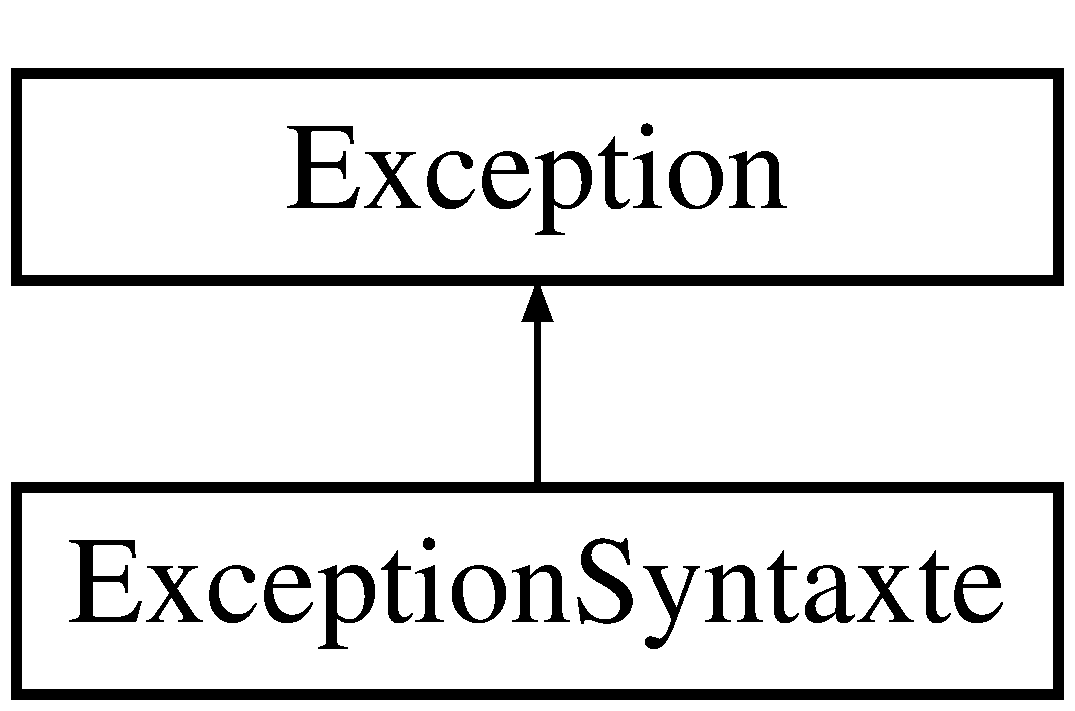
\includegraphics[height=2.000000cm]{class_exception_syntaxte}
\end{center}
\end{figure}
\subsection*{Public Types}
\begin{DoxyCompactItemize}
\item 
enum \hyperlink{class_exception_syntaxte_aca9b3139fcaa2b0101b9207fccf3d816}{Type} \{ \hyperlink{class_exception_syntaxte_aca9b3139fcaa2b0101b9207fccf3d816a6b4ad3c2fa8342e8467044175660e7f3}{S\+Y\+N\+T\+A\+X\+\_\+\+E\+R\+R\+OR}
 \}\begin{DoxyCompactList}\small\item\em Type enum correspondant. \end{DoxyCompactList}
\end{DoxyCompactItemize}
\subsection*{Public Member Functions}
\begin{DoxyCompactItemize}
\item 
\hyperlink{class_exception_syntaxte_aecef7a63420245c5b812125193a4e3f6}{Exception\+Syntaxte} (const \hyperlink{class_exception_syntaxte_aca9b3139fcaa2b0101b9207fccf3d816}{Type} t, const Q\+String \&s=\char`\"{}\char`\"{})
\begin{DoxyCompactList}\small\item\em Constructeur de l\textquotesingle{}exception. \end{DoxyCompactList}\item 
virtual \hyperlink{class_exception_syntaxte_a1f1fde8849e41fd38cb26ee97425a10d}{$\sim$\+Exception\+Syntaxte} ()\hypertarget{class_exception_syntaxte_a1f1fde8849e41fd38cb26ee97425a10d}{}\label{class_exception_syntaxte_a1f1fde8849e41fd38cb26ee97425a10d}

\begin{DoxyCompactList}\small\item\em Destructeur de l\textquotesingle{}exception. \end{DoxyCompactList}\item 
virtual const Q\+String \& \hyperlink{class_exception_syntaxte_a6bfbd6fe64c17610db8196c778e29758}{what} () const 
\begin{DoxyCompactList}\small\item\em Fonction qui retourne le message de l\textquotesingle{}exception. \end{DoxyCompactList}\item 
virtual \hyperlink{class_exception_syntaxte_aca9b3139fcaa2b0101b9207fccf3d816}{Type} \hyperlink{class_exception_syntaxte_af734fcfcfe0256aef75e48dcc886be40}{error\+Type} () const 
\begin{DoxyCompactList}\small\item\em Fonction qui retourne le type de l\textquotesingle{}exception. \end{DoxyCompactList}\end{DoxyCompactItemize}
\subsection*{Additional Inherited Members}


\subsection{Detailed Description}
Classe d\textquotesingle{}exception pour la syntaxe. 

\subsection{Member Enumeration Documentation}
\index{Exception\+Syntaxte@{Exception\+Syntaxte}!Type@{Type}}
\index{Type@{Type}!Exception\+Syntaxte@{Exception\+Syntaxte}}
\subsubsection[{\texorpdfstring{Type}{Type}}]{\setlength{\rightskip}{0pt plus 5cm}enum {\bf Exception\+Syntaxte\+::\+Type}}\hypertarget{class_exception_syntaxte_aca9b3139fcaa2b0101b9207fccf3d816}{}\label{class_exception_syntaxte_aca9b3139fcaa2b0101b9207fccf3d816}


Type enum correspondant. 

\begin{Desc}
\item[Enumerator]\par
\begin{description}
\index{S\+Y\+N\+T\+A\+X\+\_\+\+E\+R\+R\+OR@{S\+Y\+N\+T\+A\+X\+\_\+\+E\+R\+R\+OR}!Exception\+Syntaxte@{Exception\+Syntaxte}}\index{Exception\+Syntaxte@{Exception\+Syntaxte}!S\+Y\+N\+T\+A\+X\+\_\+\+E\+R\+R\+OR@{S\+Y\+N\+T\+A\+X\+\_\+\+E\+R\+R\+OR}}\item[{\em 
S\+Y\+N\+T\+A\+X\+\_\+\+E\+R\+R\+OR\hypertarget{class_exception_syntaxte_aca9b3139fcaa2b0101b9207fccf3d816a6b4ad3c2fa8342e8467044175660e7f3}{}\label{class_exception_syntaxte_aca9b3139fcaa2b0101b9207fccf3d816a6b4ad3c2fa8342e8467044175660e7f3}
}]La syntaxe est erronée \end{description}
\end{Desc}


\subsection{Constructor \& Destructor Documentation}
\index{Exception\+Syntaxte@{Exception\+Syntaxte}!Exception\+Syntaxte@{Exception\+Syntaxte}}
\index{Exception\+Syntaxte@{Exception\+Syntaxte}!Exception\+Syntaxte@{Exception\+Syntaxte}}
\subsubsection[{\texorpdfstring{Exception\+Syntaxte(const Type t, const Q\+String \&s="""")}{ExceptionSyntaxte(const Type t, const QString &s="")}}]{\setlength{\rightskip}{0pt plus 5cm}Exception\+Syntaxte\+::\+Exception\+Syntaxte (
\begin{DoxyParamCaption}
\item[{const {\bf Type}}]{t, }
\item[{const Q\+String \&}]{s = {\ttfamily \char`\"{}\char`\"{}}}
\end{DoxyParamCaption}
)\hspace{0.3cm}{\ttfamily [inline]}}\hypertarget{class_exception_syntaxte_aecef7a63420245c5b812125193a4e3f6}{}\label{class_exception_syntaxte_aecef7a63420245c5b812125193a4e3f6}


Constructeur de l\textquotesingle{}exception. 


\begin{DoxyParams}{Parameters}
{\em t} & Type de l\textquotesingle{}exception \\
\hline
{\em s} & Texte de l\textquotesingle{}exception \\
\hline
\end{DoxyParams}


\subsection{Member Function Documentation}
\index{Exception\+Syntaxte@{Exception\+Syntaxte}!error\+Type@{error\+Type}}
\index{error\+Type@{error\+Type}!Exception\+Syntaxte@{Exception\+Syntaxte}}
\subsubsection[{\texorpdfstring{error\+Type() const }{errorType() const }}]{\setlength{\rightskip}{0pt plus 5cm}virtual {\bf Type} Exception\+Syntaxte\+::error\+Type (
\begin{DoxyParamCaption}
{}
\end{DoxyParamCaption}
) const\hspace{0.3cm}{\ttfamily [inline]}, {\ttfamily [virtual]}}\hypertarget{class_exception_syntaxte_af734fcfcfe0256aef75e48dcc886be40}{}\label{class_exception_syntaxte_af734fcfcfe0256aef75e48dcc886be40}


Fonction qui retourne le type de l\textquotesingle{}exception. 

\begin{DoxyReturn}{Returns}
Le type de l\textquotesingle{}exception 
\end{DoxyReturn}
\index{Exception\+Syntaxte@{Exception\+Syntaxte}!what@{what}}
\index{what@{what}!Exception\+Syntaxte@{Exception\+Syntaxte}}
\subsubsection[{\texorpdfstring{what() const }{what() const }}]{\setlength{\rightskip}{0pt plus 5cm}virtual const Q\+String\& Exception\+Syntaxte\+::what (
\begin{DoxyParamCaption}
{}
\end{DoxyParamCaption}
) const\hspace{0.3cm}{\ttfamily [inline]}, {\ttfamily [virtual]}}\hypertarget{class_exception_syntaxte_a6bfbd6fe64c17610db8196c778e29758}{}\label{class_exception_syntaxte_a6bfbd6fe64c17610db8196c778e29758}


Fonction qui retourne le message de l\textquotesingle{}exception. 

\begin{DoxyReturn}{Returns}
Le texte de l\textquotesingle{}exception 
\end{DoxyReturn}


Implements \hyperlink{class_exception_a73ce9dfab1e48800f8818978d014c106}{Exception}.



The documentation for this class was generated from the following file\+:\begin{DoxyCompactItemize}
\item 
exception.\+h\end{DoxyCompactItemize}

\hypertarget{class_exception_wrong_type_operande}{}\section{Exception\+Wrong\+Type\+Operande Class Reference}
\label{class_exception_wrong_type_operande}\index{Exception\+Wrong\+Type\+Operande@{Exception\+Wrong\+Type\+Operande}}


Classe d\textquotesingle{}exception si une opérande est mal utilisée.  




{\ttfamily \#include $<$exception.\+h$>$}

Inheritance diagram for Exception\+Wrong\+Type\+Operande\+:\begin{figure}[H]
\begin{center}
\leavevmode
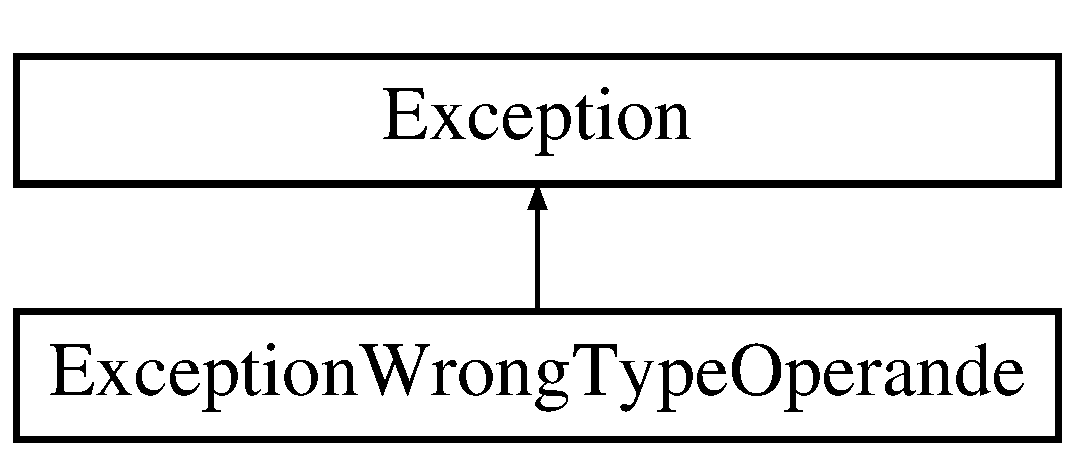
\includegraphics[height=2.000000cm]{class_exception_wrong_type_operande}
\end{center}
\end{figure}
\subsection*{Public Types}
\begin{DoxyCompactItemize}
\item 
enum \hyperlink{class_exception_wrong_type_operande_a1a1fb938febe831c80823eca12a76bd4}{Type} \{ \hyperlink{class_exception_wrong_type_operande_a1a1fb938febe831c80823eca12a76bd4ab4f913c31339309e9b0931d7ebb8a219}{W\+R\+O\+N\+G\+\_\+\+T\+Y\+P\+E\+\_\+\+O\+P\+E\+R\+A\+T\+OR}, 
\hyperlink{class_exception_wrong_type_operande_a1a1fb938febe831c80823eca12a76bd4ab13d299763581773ae9da27813cb89b9}{W\+R\+O\+N\+G\+\_\+\+T\+Y\+P\+E\+\_\+\+L\+I\+T\+T\+E\+R\+A\+LE}, 
\hyperlink{class_exception_wrong_type_operande_a1a1fb938febe831c80823eca12a76bd4acabbde7810b1e485ac025b4663e730ae}{W\+R\+O\+N\+G\+\_\+\+T\+Y\+P\+E\+\_\+\+O\+P\+E\+R\+A\+N\+DE}
 \}\begin{DoxyCompactList}\small\item\em Type enum correspondant. \end{DoxyCompactList}
\end{DoxyCompactItemize}
\subsection*{Public Member Functions}
\begin{DoxyCompactItemize}
\item 
\hyperlink{class_exception_wrong_type_operande_ae978ba3343fb4d38576350c98ece429f}{Exception\+Wrong\+Type\+Operande} (const \hyperlink{class_exception_wrong_type_operande_a1a1fb938febe831c80823eca12a76bd4}{Type} t, const Q\+String \&s=\char`\"{}\char`\"{})
\begin{DoxyCompactList}\small\item\em Constructeur de l\textquotesingle{}exception. \end{DoxyCompactList}\item 
virtual \hyperlink{class_exception_wrong_type_operande_aeb43df3eff16959457f5b1733da85667}{$\sim$\+Exception\+Wrong\+Type\+Operande} ()\hypertarget{class_exception_wrong_type_operande_aeb43df3eff16959457f5b1733da85667}{}\label{class_exception_wrong_type_operande_aeb43df3eff16959457f5b1733da85667}

\begin{DoxyCompactList}\small\item\em Destructeur de l\textquotesingle{}exception. \end{DoxyCompactList}\item 
virtual const Q\+String \& \hyperlink{class_exception_wrong_type_operande_abf65a69fad540f7015838be5576fb55d}{what} () const 
\begin{DoxyCompactList}\small\item\em Fonction qui retourne le message de l\textquotesingle{}exception. \end{DoxyCompactList}\item 
virtual \hyperlink{class_exception_wrong_type_operande_a1a1fb938febe831c80823eca12a76bd4}{Type} \hyperlink{class_exception_wrong_type_operande_abf467a4ec36bf66e7c4d2bb5876dc177}{error\+Type} () const 
\begin{DoxyCompactList}\small\item\em Fonction qui retourne le type de l\textquotesingle{}exception. \end{DoxyCompactList}\end{DoxyCompactItemize}
\subsection*{Additional Inherited Members}


\subsection{Detailed Description}
Classe d\textquotesingle{}exception si une opérande est mal utilisée. 

\subsection{Member Enumeration Documentation}
\index{Exception\+Wrong\+Type\+Operande@{Exception\+Wrong\+Type\+Operande}!Type@{Type}}
\index{Type@{Type}!Exception\+Wrong\+Type\+Operande@{Exception\+Wrong\+Type\+Operande}}
\subsubsection[{\texorpdfstring{Type}{Type}}]{\setlength{\rightskip}{0pt plus 5cm}enum {\bf Exception\+Wrong\+Type\+Operande\+::\+Type}}\hypertarget{class_exception_wrong_type_operande_a1a1fb938febe831c80823eca12a76bd4}{}\label{class_exception_wrong_type_operande_a1a1fb938febe831c80823eca12a76bd4}


Type enum correspondant. 

\begin{Desc}
\item[Enumerator]\par
\begin{description}
\index{W\+R\+O\+N\+G\+\_\+\+T\+Y\+P\+E\+\_\+\+O\+P\+E\+R\+A\+T\+OR@{W\+R\+O\+N\+G\+\_\+\+T\+Y\+P\+E\+\_\+\+O\+P\+E\+R\+A\+T\+OR}!Exception\+Wrong\+Type\+Operande@{Exception\+Wrong\+Type\+Operande}}\index{Exception\+Wrong\+Type\+Operande@{Exception\+Wrong\+Type\+Operande}!W\+R\+O\+N\+G\+\_\+\+T\+Y\+P\+E\+\_\+\+O\+P\+E\+R\+A\+T\+OR@{W\+R\+O\+N\+G\+\_\+\+T\+Y\+P\+E\+\_\+\+O\+P\+E\+R\+A\+T\+OR}}\item[{\em 
W\+R\+O\+N\+G\+\_\+\+T\+Y\+P\+E\+\_\+\+O\+P\+E\+R\+A\+T\+OR\hypertarget{class_exception_wrong_type_operande_a1a1fb938febe831c80823eca12a76bd4ab4f913c31339309e9b0931d7ebb8a219}{}\label{class_exception_wrong_type_operande_a1a1fb938febe831c80823eca12a76bd4ab4f913c31339309e9b0931d7ebb8a219}
}]L\textquotesingle{}opérateur est incorrect \index{W\+R\+O\+N\+G\+\_\+\+T\+Y\+P\+E\+\_\+\+L\+I\+T\+T\+E\+R\+A\+LE@{W\+R\+O\+N\+G\+\_\+\+T\+Y\+P\+E\+\_\+\+L\+I\+T\+T\+E\+R\+A\+LE}!Exception\+Wrong\+Type\+Operande@{Exception\+Wrong\+Type\+Operande}}\index{Exception\+Wrong\+Type\+Operande@{Exception\+Wrong\+Type\+Operande}!W\+R\+O\+N\+G\+\_\+\+T\+Y\+P\+E\+\_\+\+L\+I\+T\+T\+E\+R\+A\+LE@{W\+R\+O\+N\+G\+\_\+\+T\+Y\+P\+E\+\_\+\+L\+I\+T\+T\+E\+R\+A\+LE}}\item[{\em 
W\+R\+O\+N\+G\+\_\+\+T\+Y\+P\+E\+\_\+\+L\+I\+T\+T\+E\+R\+A\+LE\hypertarget{class_exception_wrong_type_operande_a1a1fb938febe831c80823eca12a76bd4ab13d299763581773ae9da27813cb89b9}{}\label{class_exception_wrong_type_operande_a1a1fb938febe831c80823eca12a76bd4ab13d299763581773ae9da27813cb89b9}
}]La litterale est incorrecte \index{W\+R\+O\+N\+G\+\_\+\+T\+Y\+P\+E\+\_\+\+O\+P\+E\+R\+A\+N\+DE@{W\+R\+O\+N\+G\+\_\+\+T\+Y\+P\+E\+\_\+\+O\+P\+E\+R\+A\+N\+DE}!Exception\+Wrong\+Type\+Operande@{Exception\+Wrong\+Type\+Operande}}\index{Exception\+Wrong\+Type\+Operande@{Exception\+Wrong\+Type\+Operande}!W\+R\+O\+N\+G\+\_\+\+T\+Y\+P\+E\+\_\+\+O\+P\+E\+R\+A\+N\+DE@{W\+R\+O\+N\+G\+\_\+\+T\+Y\+P\+E\+\_\+\+O\+P\+E\+R\+A\+N\+DE}}\item[{\em 
W\+R\+O\+N\+G\+\_\+\+T\+Y\+P\+E\+\_\+\+O\+P\+E\+R\+A\+N\+DE\hypertarget{class_exception_wrong_type_operande_a1a1fb938febe831c80823eca12a76bd4acabbde7810b1e485ac025b4663e730ae}{}\label{class_exception_wrong_type_operande_a1a1fb938febe831c80823eca12a76bd4acabbde7810b1e485ac025b4663e730ae}
}]L\textquotesingle{}opérande est incorrecte \end{description}
\end{Desc}


\subsection{Constructor \& Destructor Documentation}
\index{Exception\+Wrong\+Type\+Operande@{Exception\+Wrong\+Type\+Operande}!Exception\+Wrong\+Type\+Operande@{Exception\+Wrong\+Type\+Operande}}
\index{Exception\+Wrong\+Type\+Operande@{Exception\+Wrong\+Type\+Operande}!Exception\+Wrong\+Type\+Operande@{Exception\+Wrong\+Type\+Operande}}
\subsubsection[{\texorpdfstring{Exception\+Wrong\+Type\+Operande(const Type t, const Q\+String \&s="""")}{ExceptionWrongTypeOperande(const Type t, const QString &s="")}}]{\setlength{\rightskip}{0pt plus 5cm}Exception\+Wrong\+Type\+Operande\+::\+Exception\+Wrong\+Type\+Operande (
\begin{DoxyParamCaption}
\item[{const {\bf Type}}]{t, }
\item[{const Q\+String \&}]{s = {\ttfamily \char`\"{}\char`\"{}}}
\end{DoxyParamCaption}
)\hspace{0.3cm}{\ttfamily [inline]}}\hypertarget{class_exception_wrong_type_operande_ae978ba3343fb4d38576350c98ece429f}{}\label{class_exception_wrong_type_operande_ae978ba3343fb4d38576350c98ece429f}


Constructeur de l\textquotesingle{}exception. 


\begin{DoxyParams}{Parameters}
{\em t} & Type de l\textquotesingle{}exception \\
\hline
{\em s} & Texte de l\textquotesingle{}exception \\
\hline
\end{DoxyParams}


\subsection{Member Function Documentation}
\index{Exception\+Wrong\+Type\+Operande@{Exception\+Wrong\+Type\+Operande}!error\+Type@{error\+Type}}
\index{error\+Type@{error\+Type}!Exception\+Wrong\+Type\+Operande@{Exception\+Wrong\+Type\+Operande}}
\subsubsection[{\texorpdfstring{error\+Type() const }{errorType() const }}]{\setlength{\rightskip}{0pt plus 5cm}virtual {\bf Type} Exception\+Wrong\+Type\+Operande\+::error\+Type (
\begin{DoxyParamCaption}
{}
\end{DoxyParamCaption}
) const\hspace{0.3cm}{\ttfamily [inline]}, {\ttfamily [virtual]}}\hypertarget{class_exception_wrong_type_operande_abf467a4ec36bf66e7c4d2bb5876dc177}{}\label{class_exception_wrong_type_operande_abf467a4ec36bf66e7c4d2bb5876dc177}


Fonction qui retourne le type de l\textquotesingle{}exception. 

\begin{DoxyReturn}{Returns}
Le type de l\textquotesingle{}exception 
\end{DoxyReturn}
\index{Exception\+Wrong\+Type\+Operande@{Exception\+Wrong\+Type\+Operande}!what@{what}}
\index{what@{what}!Exception\+Wrong\+Type\+Operande@{Exception\+Wrong\+Type\+Operande}}
\subsubsection[{\texorpdfstring{what() const }{what() const }}]{\setlength{\rightskip}{0pt plus 5cm}virtual const Q\+String\& Exception\+Wrong\+Type\+Operande\+::what (
\begin{DoxyParamCaption}
{}
\end{DoxyParamCaption}
) const\hspace{0.3cm}{\ttfamily [inline]}, {\ttfamily [virtual]}}\hypertarget{class_exception_wrong_type_operande_abf65a69fad540f7015838be5576fb55d}{}\label{class_exception_wrong_type_operande_abf65a69fad540f7015838be5576fb55d}


Fonction qui retourne le message de l\textquotesingle{}exception. 

\begin{DoxyReturn}{Returns}
Le texte de l\textquotesingle{}exception 
\end{DoxyReturn}


Implements \hyperlink{class_exception_a73ce9dfab1e48800f8818978d014c106}{Exception}.



The documentation for this class was generated from the following file\+:\begin{DoxyCompactItemize}
\item 
exception.\+h\end{DoxyCompactItemize}

\hypertarget{class_litterale}{}\section{Litterale Class Reference}
\label{class_litterale}\index{Litterale@{Litterale}}


Classe mère de toutes les litterales (abstraite)  




{\ttfamily \#include $<$litterale.\+h$>$}

Inheritance diagram for Litterale\+:\begin{figure}[H]
\begin{center}
\leavevmode
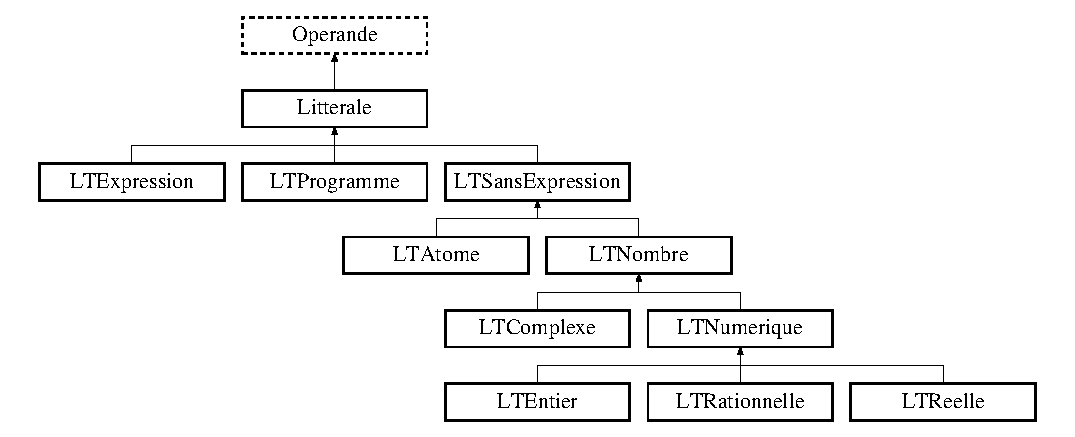
\includegraphics[height=5.419354cm]{class_litterale}
\end{center}
\end{figure}
\subsection*{Public Member Functions}
\begin{DoxyCompactItemize}
\item 
\hyperlink{class_litterale_aa0a02717ec75f502f1afdb6ac597efac}{Litterale} ()\hypertarget{class_litterale_aa0a02717ec75f502f1afdb6ac597efac}{}\label{class_litterale_aa0a02717ec75f502f1afdb6ac597efac}

\begin{DoxyCompactList}\small\item\em Constructeur. \end{DoxyCompactList}\item 
virtual \hyperlink{class_litterale_abd6b3faa8cda262bb5fab57e1e323090}{$\sim$\+Litterale} ()\hypertarget{class_litterale_abd6b3faa8cda262bb5fab57e1e323090}{}\label{class_litterale_abd6b3faa8cda262bb5fab57e1e323090}

\begin{DoxyCompactList}\small\item\em Destructeur. \end{DoxyCompactList}\item 
virtual \hyperlink{class_litterale}{Litterale} $\ast$ \hyperlink{class_litterale_a08967178d22c3d69e6c3e86ea8c85888}{clone} () const  =0
\begin{DoxyCompactList}\small\item\em Fonction virtuelle renvoyant une copie de l\textquotesingle{}instance. \end{DoxyCompactList}\item 
virtual \hyperlink{class_litterale}{Litterale} $\ast$ \hyperlink{class_litterale_af33a0c1a4a9a5bb687da112b12f0e6e6}{simplifier} ()=0
\begin{DoxyCompactList}\small\item\em Fonction virtuelle simplifiant la litterale actuelle. \end{DoxyCompactList}\item 
virtual Q\+String \hyperlink{class_litterale_a780075c00abf31efb87e7c28843ea029}{get\+Text} () const  =0
\begin{DoxyCompactList}\small\item\em Fonction virtuelle renvoyant la litterale sous forme de texte. \end{DoxyCompactList}\item 
virtual void \hyperlink{class_litterale_aa63aae17689258434f4a1319b7371571}{afficher} () const  =0\hypertarget{class_litterale_aa63aae17689258434f4a1319b7371571}{}\label{class_litterale_aa63aae17689258434f4a1319b7371571}

\begin{DoxyCompactList}\small\item\em Fonction virtuelle affichant la litterale sur la sortie standart. \end{DoxyCompactList}\end{DoxyCompactItemize}


\subsection{Detailed Description}
Classe mère de toutes les litterales (abstraite) 

\subsection{Member Function Documentation}
\index{Litterale@{Litterale}!clone@{clone}}
\index{clone@{clone}!Litterale@{Litterale}}
\subsubsection[{\texorpdfstring{clone() const  =0}{clone() const  =0}}]{\setlength{\rightskip}{0pt plus 5cm}virtual {\bf Litterale}$\ast$ Litterale\+::clone (
\begin{DoxyParamCaption}
{}
\end{DoxyParamCaption}
) const\hspace{0.3cm}{\ttfamily [pure virtual]}}\hypertarget{class_litterale_a08967178d22c3d69e6c3e86ea8c85888}{}\label{class_litterale_a08967178d22c3d69e6c3e86ea8c85888}


Fonction virtuelle renvoyant une copie de l\textquotesingle{}instance. 

\begin{DoxyReturn}{Returns}
Nouvelle litterale copiée 
\end{DoxyReturn}


Implements \hyperlink{class_operande}{Operande}.



Implemented in \hyperlink{class_l_t_reelle_a1dac7c02dfa84815730d5f0396ef1519}{L\+T\+Reelle}, \hyperlink{class_l_t_rationnelle_a48b36c50460ce15674d1d72afb41daf3}{L\+T\+Rationnelle}, \hyperlink{class_l_t_entier_afc21b025efd3feea0162053902b8d640}{L\+T\+Entier}, \hyperlink{class_l_t_atome_a8fd75a87781e2544fb090da6096a7106}{L\+T\+Atome}, \hyperlink{class_l_t_complexe_ae597257b1e7b81ad6914e44b616c006d}{L\+T\+Complexe}, \hyperlink{class_l_t_expression_ab51c526b6232a131bea9a43945633b2a}{L\+T\+Expression}, \hyperlink{class_l_t_numerique_a884056443dd30cd71c49b42b5ba63581}{L\+T\+Numerique}, \hyperlink{class_l_t_programme_a1ae271a87f8b770aec069aa6dec3b84b}{L\+T\+Programme}, \hyperlink{class_l_t_nombre_a09ad6faddbb007746e41af6873bd1824}{L\+T\+Nombre}, and \hyperlink{class_l_t_sans_expression_af0299c947bb7a910ddd4c419cf729313}{L\+T\+Sans\+Expression}.

\index{Litterale@{Litterale}!get\+Text@{get\+Text}}
\index{get\+Text@{get\+Text}!Litterale@{Litterale}}
\subsubsection[{\texorpdfstring{get\+Text() const  =0}{getText() const  =0}}]{\setlength{\rightskip}{0pt plus 5cm}virtual Q\+String Litterale\+::get\+Text (
\begin{DoxyParamCaption}
{}
\end{DoxyParamCaption}
) const\hspace{0.3cm}{\ttfamily [pure virtual]}}\hypertarget{class_litterale_a780075c00abf31efb87e7c28843ea029}{}\label{class_litterale_a780075c00abf31efb87e7c28843ea029}


Fonction virtuelle renvoyant la litterale sous forme de texte. 

\begin{DoxyReturn}{Returns}
\hyperlink{class_litterale}{Litterale} sous forme de texte 
\end{DoxyReturn}


Implements \hyperlink{class_operande}{Operande}.



Implemented in \hyperlink{class_l_t_reelle_aa85d99c6c692e3fd51019630cfd88cc4}{L\+T\+Reelle}, \hyperlink{class_l_t_rationnelle_a7195f7e7ddfe6c5493932fe08785ac76}{L\+T\+Rationnelle}, \hyperlink{class_l_t_entier_a735c05de25b1264a5b2bc603f63eed58}{L\+T\+Entier}, \hyperlink{class_l_t_atome_a2140a7071f7d1d5ddca671802de17447}{L\+T\+Atome}, \hyperlink{class_l_t_complexe_a25992476892bbc3a33ea61dba8bc9160}{L\+T\+Complexe}, \hyperlink{class_l_t_expression_a13d5a9d4a536ed34effcb08a6e5391a6}{L\+T\+Expression}, \hyperlink{class_l_t_numerique_abef28b1b62ee356717f70f4317a44590}{L\+T\+Numerique}, \hyperlink{class_l_t_nombre_a39fe941ec69bf013bc3be8b3e575c3d0}{L\+T\+Nombre}, \hyperlink{class_l_t_programme_ad5f8e3d531b8a456944d806096881022}{L\+T\+Programme}, and \hyperlink{class_l_t_sans_expression_a4f0372c490b49bfc654e394a59c4c015}{L\+T\+Sans\+Expression}.

\index{Litterale@{Litterale}!simplifier@{simplifier}}
\index{simplifier@{simplifier}!Litterale@{Litterale}}
\subsubsection[{\texorpdfstring{simplifier()=0}{simplifier()=0}}]{\setlength{\rightskip}{0pt plus 5cm}virtual {\bf Litterale}$\ast$ Litterale\+::simplifier (
\begin{DoxyParamCaption}
{}
\end{DoxyParamCaption}
)\hspace{0.3cm}{\ttfamily [pure virtual]}}\hypertarget{class_litterale_af33a0c1a4a9a5bb687da112b12f0e6e6}{}\label{class_litterale_af33a0c1a4a9a5bb687da112b12f0e6e6}


Fonction virtuelle simplifiant la litterale actuelle. 

\begin{DoxyReturn}{Returns}
Nouvelle litterale copiée 
\end{DoxyReturn}


Implemented in \hyperlink{class_l_t_reelle_aaaf23323d16d13b2ec7595c6aa07935f}{L\+T\+Reelle}, \hyperlink{class_l_t_rationnelle_afefcccb71e7fd20491e8f14aef88dd6e}{L\+T\+Rationnelle}, \hyperlink{class_l_t_entier_a3dd0959762240ef5cbe0a62970728ddf}{L\+T\+Entier}, \hyperlink{class_l_t_atome_a2e2cee64c687ab8c648e4866ab1150b8}{L\+T\+Atome}, \hyperlink{class_l_t_complexe_aa4781a2130c4dd2daa81fde8caa6fff3}{L\+T\+Complexe}, \hyperlink{class_l_t_expression_a8817e6f26189ad7a4e65bd24f6020367}{L\+T\+Expression}, \hyperlink{class_l_t_numerique_a3963de62916188d01f93b1d0fdb42c7f}{L\+T\+Numerique}, \hyperlink{class_l_t_programme_a7bfe6b6140e56fc578ed5dce2e2d9ea5}{L\+T\+Programme}, \hyperlink{class_l_t_nombre_a6aa1593c8c0956bb5412bfee3c15b085}{L\+T\+Nombre}, and \hyperlink{class_l_t_sans_expression_a13982a6a4f155bac50a0058a2c352e91}{L\+T\+Sans\+Expression}.



The documentation for this class was generated from the following file\+:\begin{DoxyCompactItemize}
\item 
litterale.\+h\end{DoxyCompactItemize}

\hypertarget{class_l_t_atome}{}\section{L\+T\+Atome Class Reference}
\label{class_l_t_atome}\index{L\+T\+Atome@{L\+T\+Atome}}


Classe d\textquotesingle{}une litterale atome.  




{\ttfamily \#include $<$ltatome.\+h$>$}

Inheritance diagram for L\+T\+Atome\+:\begin{figure}[H]
\begin{center}
\leavevmode
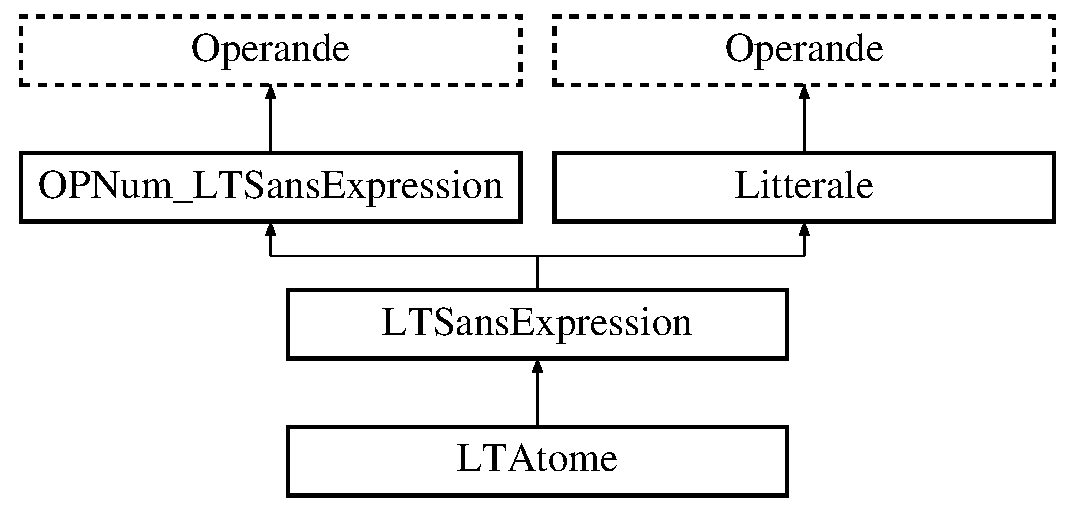
\includegraphics[height=4.000000cm]{class_l_t_atome}
\end{center}
\end{figure}
\subsection*{Public Types}
\begin{DoxyCompactItemize}
\item 
enum \hyperlink{class_l_t_atome_a340480fc682a6d8fd819026d20278b49}{Enum\+Nature} \{ \hyperlink{class_l_t_atome_a340480fc682a6d8fd819026d20278b49a99911d63d6cb7a762dfeec132628ff22}{I\+D\+V\+AR}, 
\hyperlink{class_l_t_atome_a340480fc682a6d8fd819026d20278b49a56cc525550a6a682752d67bd704f834a}{I\+D\+P\+R\+OG}, 
\hyperlink{class_l_t_atome_a340480fc682a6d8fd819026d20278b49a192a6fae9192e3a133b23f9939bcebd3}{I\+D\+E\+XP}, 
\hyperlink{class_l_t_atome_a340480fc682a6d8fd819026d20278b49a841226cd2ef78fa4c11c33180b05103e}{I\+N\+D\+E\+F\+I\+NI}
 \}\begin{DoxyCompactList}\small\item\em Enum concernant la nature de l\textquotesingle{}atome. \end{DoxyCompactList}
\end{DoxyCompactItemize}
\subsection*{Public Member Functions}
\begin{DoxyCompactItemize}
\item 
\hyperlink{class_l_t_atome_a533e5d85b12e1a9e902cc7d29c58868a}{L\+T\+Atome} (Q\+String v, \hyperlink{class_l_t_atome_a340480fc682a6d8fd819026d20278b49}{Enum\+Nature} n, \hyperlink{class_litterale}{Litterale} $\ast$p=nullptr)
\begin{DoxyCompactList}\small\item\em Constructeur de l\textquotesingle{}atome. \end{DoxyCompactList}\item 
\hyperlink{class_l_t_atome_a8b3d9c68655bf64d0924e892922c77f2}{L\+T\+Atome} (Q\+String v, \hyperlink{class_litterale}{Litterale} $\ast$p=nullptr)
\begin{DoxyCompactList}\small\item\em Constructeur de l\textquotesingle{}atome. \end{DoxyCompactList}\item 
virtual \hyperlink{class_l_t_atome_aff1cf3e8e7f7b6f0fcc7818e832ecd08}{$\sim$\+L\+T\+Atome} ()\hypertarget{class_l_t_atome_aff1cf3e8e7f7b6f0fcc7818e832ecd08}{}\label{class_l_t_atome_aff1cf3e8e7f7b6f0fcc7818e832ecd08}

\begin{DoxyCompactList}\small\item\em Destructeur de l\textquotesingle{}atome. \end{DoxyCompactList}\item 
void \hyperlink{class_l_t_atome_acede21b7dde27b0973b3a9de0db6ad40}{set\+Pointer} (\hyperlink{class_litterale}{Litterale} $\ast$l)
\begin{DoxyCompactList}\small\item\em Définir la litterale pointée par l\textquotesingle{}atome. \end{DoxyCompactList}\item 
\hyperlink{class_l_t_atome_a340480fc682a6d8fd819026d20278b49}{Enum\+Nature} \hyperlink{class_l_t_atome_af0794b76e812f3918b47fedd95e06eae}{get\+Nature} () const 
\begin{DoxyCompactList}\small\item\em Renvoie la nature de l\textquotesingle{}atome. \end{DoxyCompactList}\item 
\hyperlink{class_litterale}{Litterale} $\ast$ \hyperlink{class_l_t_atome_a495b6dbfaa0e2ebd997f969fbaa2015e}{get\+Pointer} () const 
\begin{DoxyCompactList}\small\item\em Renvoie la litterale pointée par l\textquotesingle{}atome. \end{DoxyCompactList}\item 
Q\+String \hyperlink{class_l_t_atome_ae6acabae4ebfbaa0d36e184b63647b63}{get\+Enum\+String} () const 
\begin{DoxyCompactList}\small\item\em Renvoie la nature de l\textquotesingle{}atome au format texte. \end{DoxyCompactList}\item 
virtual void \hyperlink{class_l_t_atome_a4ab2828d23dc388e567522485bdebfe6}{afficher} () const \hypertarget{class_l_t_atome_a4ab2828d23dc388e567522485bdebfe6}{}\label{class_l_t_atome_a4ab2828d23dc388e567522485bdebfe6}

\begin{DoxyCompactList}\small\item\em Fonction d\textquotesingle{}affichage. \end{DoxyCompactList}\item 
Q\+String \hyperlink{class_l_t_atome_a2140a7071f7d1d5ddca671802de17447}{get\+Text} () const 
\begin{DoxyCompactList}\small\item\em Getter de l\textquotesingle{}identifiant au format texte. \end{DoxyCompactList}\item 
Q\+String \hyperlink{class_l_t_atome_a814a35a047dc21cc912a06789919973d}{get\+Name} () const 
\begin{DoxyCompactList}\small\item\em Getter de l\textquotesingle{}identifiant au format texte. \end{DoxyCompactList}\item 
virtual \hyperlink{class_l_t_atome}{L\+T\+Atome} $\ast$ \hyperlink{class_l_t_atome_a8fd75a87781e2544fb090da6096a7106}{clone} () const 
\begin{DoxyCompactList}\small\item\em Fonction virtuelle renvoyant une copie de l\textquotesingle{}instance. \end{DoxyCompactList}\item 
virtual \hyperlink{class_litterale}{Litterale} $\ast$ \hyperlink{class_l_t_atome_a2e2cee64c687ab8c648e4866ab1150b8}{simplifier} ()
\begin{DoxyCompactList}\small\item\em Fonction virtuelle simplifiant la litterale actuelle. \end{DoxyCompactList}\end{DoxyCompactItemize}
\subsection*{Static Public Member Functions}
\begin{DoxyCompactItemize}
\item 
static \hyperlink{class_l_t_atome_a340480fc682a6d8fd819026d20278b49}{Enum\+Nature} \hyperlink{class_l_t_atome_aa684a663ff7ac9011903eb6bd43593af}{Enum\+From\+String} (const Q\+String \&text)
\begin{DoxyCompactList}\small\item\em Renvoie une nature en fonction d\textquotesingle{}un texte. \end{DoxyCompactList}\end{DoxyCompactItemize}


\subsection{Detailed Description}
Classe d\textquotesingle{}une litterale atome. 

\subsection{Member Enumeration Documentation}
\index{L\+T\+Atome@{L\+T\+Atome}!Enum\+Nature@{Enum\+Nature}}
\index{Enum\+Nature@{Enum\+Nature}!L\+T\+Atome@{L\+T\+Atome}}
\subsubsection[{\texorpdfstring{Enum\+Nature}{EnumNature}}]{\setlength{\rightskip}{0pt plus 5cm}enum {\bf L\+T\+Atome\+::\+Enum\+Nature}}\hypertarget{class_l_t_atome_a340480fc682a6d8fd819026d20278b49}{}\label{class_l_t_atome_a340480fc682a6d8fd819026d20278b49}


Enum concernant la nature de l\textquotesingle{}atome. 

\begin{Desc}
\item[Enumerator]\par
\begin{description}
\index{I\+D\+V\+AR@{I\+D\+V\+AR}!L\+T\+Atome@{L\+T\+Atome}}\index{L\+T\+Atome@{L\+T\+Atome}!I\+D\+V\+AR@{I\+D\+V\+AR}}\item[{\em 
I\+D\+V\+AR\hypertarget{class_l_t_atome_a340480fc682a6d8fd819026d20278b49a99911d63d6cb7a762dfeec132628ff22}{}\label{class_l_t_atome_a340480fc682a6d8fd819026d20278b49a99911d63d6cb7a762dfeec132628ff22}
}]Identificateur d\textquotesingle{}une variable \index{I\+D\+P\+R\+OG@{I\+D\+P\+R\+OG}!L\+T\+Atome@{L\+T\+Atome}}\index{L\+T\+Atome@{L\+T\+Atome}!I\+D\+P\+R\+OG@{I\+D\+P\+R\+OG}}\item[{\em 
I\+D\+P\+R\+OG\hypertarget{class_l_t_atome_a340480fc682a6d8fd819026d20278b49a56cc525550a6a682752d67bd704f834a}{}\label{class_l_t_atome_a340480fc682a6d8fd819026d20278b49a56cc525550a6a682752d67bd704f834a}
}]Identificateur d\textquotesingle{}un programme \index{I\+D\+E\+XP@{I\+D\+E\+XP}!L\+T\+Atome@{L\+T\+Atome}}\index{L\+T\+Atome@{L\+T\+Atome}!I\+D\+E\+XP@{I\+D\+E\+XP}}\item[{\em 
I\+D\+E\+XP\hypertarget{class_l_t_atome_a340480fc682a6d8fd819026d20278b49a192a6fae9192e3a133b23f9939bcebd3}{}\label{class_l_t_atome_a340480fc682a6d8fd819026d20278b49a192a6fae9192e3a133b23f9939bcebd3}
}]Identificateur d\textquotesingle{}une expression \index{I\+N\+D\+E\+F\+I\+NI@{I\+N\+D\+E\+F\+I\+NI}!L\+T\+Atome@{L\+T\+Atome}}\index{L\+T\+Atome@{L\+T\+Atome}!I\+N\+D\+E\+F\+I\+NI@{I\+N\+D\+E\+F\+I\+NI}}\item[{\em 
I\+N\+D\+E\+F\+I\+NI\hypertarget{class_l_t_atome_a340480fc682a6d8fd819026d20278b49a841226cd2ef78fa4c11c33180b05103e}{}\label{class_l_t_atome_a340480fc682a6d8fd819026d20278b49a841226cd2ef78fa4c11c33180b05103e}
}]Identificateur indéfini \end{description}
\end{Desc}


\subsection{Constructor \& Destructor Documentation}
\index{L\+T\+Atome@{L\+T\+Atome}!L\+T\+Atome@{L\+T\+Atome}}
\index{L\+T\+Atome@{L\+T\+Atome}!L\+T\+Atome@{L\+T\+Atome}}
\subsubsection[{\texorpdfstring{L\+T\+Atome(\+Q\+String v, Enum\+Nature n, Litterale $\ast$p=nullptr)}{LTAtome(QString v, EnumNature n, Litterale *p=nullptr)}}]{\setlength{\rightskip}{0pt plus 5cm}L\+T\+Atome\+::\+L\+T\+Atome (
\begin{DoxyParamCaption}
\item[{Q\+String}]{v, }
\item[{{\bf Enum\+Nature}}]{n, }
\item[{{\bf Litterale} $\ast$}]{p = {\ttfamily nullptr}}
\end{DoxyParamCaption}
)\hspace{0.3cm}{\ttfamily [inline]}}\hypertarget{class_l_t_atome_a533e5d85b12e1a9e902cc7d29c58868a}{}\label{class_l_t_atome_a533e5d85b12e1a9e902cc7d29c58868a}


Constructeur de l\textquotesingle{}atome. 


\begin{DoxyParams}{Parameters}
{\em v} & Nom de l\textquotesingle{}atome \\
\hline
{\em n} & Nature de l\textquotesingle{}atome \\
\hline
{\em p} & \hyperlink{class_litterale}{Litterale} associée \\
\hline
\end{DoxyParams}
\index{L\+T\+Atome@{L\+T\+Atome}!L\+T\+Atome@{L\+T\+Atome}}
\index{L\+T\+Atome@{L\+T\+Atome}!L\+T\+Atome@{L\+T\+Atome}}
\subsubsection[{\texorpdfstring{L\+T\+Atome(\+Q\+String v, Litterale $\ast$p=nullptr)}{LTAtome(QString v, Litterale *p=nullptr)}}]{\setlength{\rightskip}{0pt plus 5cm}L\+T\+Atome\+::\+L\+T\+Atome (
\begin{DoxyParamCaption}
\item[{Q\+String}]{v, }
\item[{{\bf Litterale} $\ast$}]{p = {\ttfamily nullptr}}
\end{DoxyParamCaption}
)\hspace{0.3cm}{\ttfamily [inline]}}\hypertarget{class_l_t_atome_a8b3d9c68655bf64d0924e892922c77f2}{}\label{class_l_t_atome_a8b3d9c68655bf64d0924e892922c77f2}


Constructeur de l\textquotesingle{}atome. 


\begin{DoxyParams}{Parameters}
{\em v} & Nom de l\textquotesingle{}atome \\
\hline
{\em p} & \hyperlink{class_litterale}{Litterale} associée \\
\hline
\end{DoxyParams}


\subsection{Member Function Documentation}
\index{L\+T\+Atome@{L\+T\+Atome}!clone@{clone}}
\index{clone@{clone}!L\+T\+Atome@{L\+T\+Atome}}
\subsubsection[{\texorpdfstring{clone() const }{clone() const }}]{\setlength{\rightskip}{0pt plus 5cm}virtual {\bf L\+T\+Atome}$\ast$ L\+T\+Atome\+::clone (
\begin{DoxyParamCaption}
{}
\end{DoxyParamCaption}
) const\hspace{0.3cm}{\ttfamily [inline]}, {\ttfamily [virtual]}}\hypertarget{class_l_t_atome_a8fd75a87781e2544fb090da6096a7106}{}\label{class_l_t_atome_a8fd75a87781e2544fb090da6096a7106}


Fonction virtuelle renvoyant une copie de l\textquotesingle{}instance. 

\begin{DoxyReturn}{Returns}
Nouvelle litterale copiée 
\end{DoxyReturn}


Implements \hyperlink{class_l_t_sans_expression_af0299c947bb7a910ddd4c419cf729313}{L\+T\+Sans\+Expression}.

\index{L\+T\+Atome@{L\+T\+Atome}!Enum\+From\+String@{Enum\+From\+String}}
\index{Enum\+From\+String@{Enum\+From\+String}!L\+T\+Atome@{L\+T\+Atome}}
\subsubsection[{\texorpdfstring{Enum\+From\+String(const Q\+String \&text)}{EnumFromString(const QString &text)}}]{\setlength{\rightskip}{0pt plus 5cm}static {\bf Enum\+Nature} L\+T\+Atome\+::\+Enum\+From\+String (
\begin{DoxyParamCaption}
\item[{const Q\+String \&}]{text}
\end{DoxyParamCaption}
)\hspace{0.3cm}{\ttfamily [inline]}, {\ttfamily [static]}}\hypertarget{class_l_t_atome_aa684a663ff7ac9011903eb6bd43593af}{}\label{class_l_t_atome_aa684a663ff7ac9011903eb6bd43593af}


Renvoie une nature en fonction d\textquotesingle{}un texte. 


\begin{DoxyParams}{Parameters}
{\em p} & Nature de l\textquotesingle{}atome au format Texte \\
\hline
\end{DoxyParams}
\begin{DoxyReturn}{Returns}
Nature de l\textquotesingle{}atome au format Enum 
\end{DoxyReturn}
\index{L\+T\+Atome@{L\+T\+Atome}!get\+Enum\+String@{get\+Enum\+String}}
\index{get\+Enum\+String@{get\+Enum\+String}!L\+T\+Atome@{L\+T\+Atome}}
\subsubsection[{\texorpdfstring{get\+Enum\+String() const }{getEnumString() const }}]{\setlength{\rightskip}{0pt plus 5cm}Q\+String L\+T\+Atome\+::get\+Enum\+String (
\begin{DoxyParamCaption}
{}
\end{DoxyParamCaption}
) const\hspace{0.3cm}{\ttfamily [inline]}}\hypertarget{class_l_t_atome_ae6acabae4ebfbaa0d36e184b63647b63}{}\label{class_l_t_atome_ae6acabae4ebfbaa0d36e184b63647b63}


Renvoie la nature de l\textquotesingle{}atome au format texte. 

\begin{DoxyReturn}{Returns}
Nature de l\textquotesingle{}atome au format texte 
\end{DoxyReturn}
\index{L\+T\+Atome@{L\+T\+Atome}!get\+Name@{get\+Name}}
\index{get\+Name@{get\+Name}!L\+T\+Atome@{L\+T\+Atome}}
\subsubsection[{\texorpdfstring{get\+Name() const }{getName() const }}]{\setlength{\rightskip}{0pt plus 5cm}Q\+String L\+T\+Atome\+::get\+Name (
\begin{DoxyParamCaption}
{}
\end{DoxyParamCaption}
) const\hspace{0.3cm}{\ttfamily [inline]}}\hypertarget{class_l_t_atome_a814a35a047dc21cc912a06789919973d}{}\label{class_l_t_atome_a814a35a047dc21cc912a06789919973d}


Getter de l\textquotesingle{}identifiant au format texte. 

\begin{DoxyReturn}{Returns}
Renvoie la propriété value 
\end{DoxyReturn}
\index{L\+T\+Atome@{L\+T\+Atome}!get\+Nature@{get\+Nature}}
\index{get\+Nature@{get\+Nature}!L\+T\+Atome@{L\+T\+Atome}}
\subsubsection[{\texorpdfstring{get\+Nature() const }{getNature() const }}]{\setlength{\rightskip}{0pt plus 5cm}{\bf L\+T\+Atome\+::\+Enum\+Nature} L\+T\+Atome\+::get\+Nature (
\begin{DoxyParamCaption}
{}
\end{DoxyParamCaption}
) const}\hypertarget{class_l_t_atome_af0794b76e812f3918b47fedd95e06eae}{}\label{class_l_t_atome_af0794b76e812f3918b47fedd95e06eae}


Renvoie la nature de l\textquotesingle{}atome. 

\begin{DoxyReturn}{Returns}
Nature de l\textquotesingle{}atome 
\end{DoxyReturn}
\index{L\+T\+Atome@{L\+T\+Atome}!get\+Pointer@{get\+Pointer}}
\index{get\+Pointer@{get\+Pointer}!L\+T\+Atome@{L\+T\+Atome}}
\subsubsection[{\texorpdfstring{get\+Pointer() const }{getPointer() const }}]{\setlength{\rightskip}{0pt plus 5cm}{\bf Litterale} $\ast$ L\+T\+Atome\+::get\+Pointer (
\begin{DoxyParamCaption}
{}
\end{DoxyParamCaption}
) const}\hypertarget{class_l_t_atome_a495b6dbfaa0e2ebd997f969fbaa2015e}{}\label{class_l_t_atome_a495b6dbfaa0e2ebd997f969fbaa2015e}


Renvoie la litterale pointée par l\textquotesingle{}atome. 

\begin{DoxyReturn}{Returns}
\hyperlink{class_litterale}{Litterale} pointée par l\textquotesingle{}atome 
\end{DoxyReturn}
\index{L\+T\+Atome@{L\+T\+Atome}!get\+Text@{get\+Text}}
\index{get\+Text@{get\+Text}!L\+T\+Atome@{L\+T\+Atome}}
\subsubsection[{\texorpdfstring{get\+Text() const }{getText() const }}]{\setlength{\rightskip}{0pt plus 5cm}Q\+String L\+T\+Atome\+::get\+Text (
\begin{DoxyParamCaption}
{}
\end{DoxyParamCaption}
) const\hspace{0.3cm}{\ttfamily [inline]}, {\ttfamily [virtual]}}\hypertarget{class_l_t_atome_a2140a7071f7d1d5ddca671802de17447}{}\label{class_l_t_atome_a2140a7071f7d1d5ddca671802de17447}


Getter de l\textquotesingle{}identifiant au format texte. 

\begin{DoxyReturn}{Returns}
Renvoie la propriété value 
\end{DoxyReturn}


Implements \hyperlink{class_l_t_sans_expression_a4f0372c490b49bfc654e394a59c4c015}{L\+T\+Sans\+Expression}.

\index{L\+T\+Atome@{L\+T\+Atome}!set\+Pointer@{set\+Pointer}}
\index{set\+Pointer@{set\+Pointer}!L\+T\+Atome@{L\+T\+Atome}}
\subsubsection[{\texorpdfstring{set\+Pointer(\+Litterale $\ast$l)}{setPointer(Litterale *l)}}]{\setlength{\rightskip}{0pt plus 5cm}void L\+T\+Atome\+::set\+Pointer (
\begin{DoxyParamCaption}
\item[{{\bf Litterale} $\ast$}]{l}
\end{DoxyParamCaption}
)}\hypertarget{class_l_t_atome_acede21b7dde27b0973b3a9de0db6ad40}{}\label{class_l_t_atome_acede21b7dde27b0973b3a9de0db6ad40}


Définir la litterale pointée par l\textquotesingle{}atome. 


\begin{DoxyParams}{Parameters}
{\em l} & \hyperlink{class_litterale}{Litterale} pointée par l\textquotesingle{}atome \\
\hline
\end{DoxyParams}
\index{L\+T\+Atome@{L\+T\+Atome}!simplifier@{simplifier}}
\index{simplifier@{simplifier}!L\+T\+Atome@{L\+T\+Atome}}
\subsubsection[{\texorpdfstring{simplifier()}{simplifier()}}]{\setlength{\rightskip}{0pt plus 5cm}virtual {\bf Litterale}$\ast$ L\+T\+Atome\+::simplifier (
\begin{DoxyParamCaption}
{}
\end{DoxyParamCaption}
)\hspace{0.3cm}{\ttfamily [inline]}, {\ttfamily [virtual]}}\hypertarget{class_l_t_atome_a2e2cee64c687ab8c648e4866ab1150b8}{}\label{class_l_t_atome_a2e2cee64c687ab8c648e4866ab1150b8}


Fonction virtuelle simplifiant la litterale actuelle. 

\begin{DoxyReturn}{Returns}
Nouvelle litterale copiée 
\end{DoxyReturn}


Implements \hyperlink{class_l_t_sans_expression_a13982a6a4f155bac50a0058a2c352e91}{L\+T\+Sans\+Expression}.



The documentation for this class was generated from the following files\+:\begin{DoxyCompactItemize}
\item 
ltatome.\+h\item 
ltatome.\+cpp\end{DoxyCompactItemize}

\hypertarget{class_l_t_atome_manager}{}\section{L\+T\+Atome\+Manager Class Reference}
\label{class_l_t_atome_manager}\index{L\+T\+Atome\+Manager@{L\+T\+Atome\+Manager}}


Classe \hyperlink{class_l_t_atome_manager}{L\+T\+Atome\+Manager} (Singleton) \+: factory d\textquotesingle{}atome, gère leur création, notamment les cas où un atome du même nom existe déjà  




{\ttfamily \#include $<$ltatomemanager.\+h$>$}

\subsection*{Public Member Functions}
\begin{DoxyCompactItemize}
\item 
\hyperlink{class_litterale}{Litterale} $\ast$ \hyperlink{class_l_t_atome_manager_a56939fbd4c4200c169d5cc5033d5cb31}{create\+Atome\+Or\+Associated\+Litterale} (Q\+String name, \hyperlink{class_l_t_atome_a340480fc682a6d8fd819026d20278b49}{L\+T\+Atome\+::\+Enum\+Nature} n=L\+T\+Atome\+::\+Enum\+Nature\+::\+I\+N\+D\+E\+F\+I\+NI)
\begin{DoxyCompactList}\small\item\em Permet de créer un atome ou de renvoyer la litterale associée à l\textquotesingle{}atome considéré \end{DoxyCompactList}\item 
\hyperlink{class_l_t_atome}{L\+T\+Atome} $\ast$ \hyperlink{class_l_t_atome_manager_a54aa2976d7890586510eb5c5ba0e286e}{create\+Atome} (Q\+String name, \hyperlink{class_l_t_atome_a340480fc682a6d8fd819026d20278b49}{L\+T\+Atome\+::\+Enum\+Nature} n=L\+T\+Atome\+::\+Enum\+Nature\+::\+I\+N\+D\+E\+F\+I\+NI)
\begin{DoxyCompactList}\small\item\em Fonction qui permet de créer un atome. \end{DoxyCompactList}\item 
\hyperlink{class_l_t_expression}{L\+T\+Expression} $\ast$ \hyperlink{class_l_t_atome_manager_a94b3cee113aa00c935478ae35a4d48ef}{expression\+From\+Atome} (\hyperlink{class_l_t_atome}{L\+T\+Atome} $\ast$a)
\begin{DoxyCompactList}\small\item\em Créé une expression à partir d\textquotesingle{}un atome. \end{DoxyCompactList}\item 
void \hyperlink{class_l_t_atome_manager_a8331ed1c68938aa1b7f53460811b8149}{remove\+Atome} (\hyperlink{class_l_t_atome}{L\+T\+Atome} $\ast$a)
\begin{DoxyCompactList}\small\item\em Suppression d\textquotesingle{}un atome. \end{DoxyCompactList}\item 
void \hyperlink{class_l_t_atome_manager_a1177ea9fc37d29a4f97a9d80ba057060}{save\+In\+File} ()\hypertarget{class_l_t_atome_manager_a1177ea9fc37d29a4f97a9d80ba057060}{}\label{class_l_t_atome_manager_a1177ea9fc37d29a4f97a9d80ba057060}

\begin{DoxyCompactList}\small\item\em Sauvegarde dans un fichier X\+ML l\textquotesingle{}ensemble des atomes, leur valeur et les litterales associées. \end{DoxyCompactList}\item 
Q\+Map$<$ Q\+String, \hyperlink{class_l_t_atome}{L\+T\+Atome} $\ast$ $>$ \hyperlink{class_l_t_atome_manager_a9c7bc8f2fac1077d598d46c9d8a2d45d}{get\+Dictionnary} ()
\begin{DoxyCompactList}\small\item\em Renvoie le map contenant les identifiants et les atomes associés. \end{DoxyCompactList}\item 
void \hyperlink{class_l_t_atome_manager_ad172ad7d721b601757ec52ac63015806}{append\+To\+Dictionnary} (Q\+Map$<$ Q\+String, \hyperlink{class_l_t_atome}{L\+T\+Atome} $\ast$ $>$ dic)
\begin{DoxyCompactList}\small\item\em Ajouter une liste d\textquotesingle{}élément dans la map. \end{DoxyCompactList}\item 
void \hyperlink{class_l_t_atome_manager_a28b0da19fc580b243efc9f12251ee19a}{remove\+All\+From\+Dictionnary} ()\hypertarget{class_l_t_atome_manager_a28b0da19fc580b243efc9f12251ee19a}{}\label{class_l_t_atome_manager_a28b0da19fc580b243efc9f12251ee19a}

\begin{DoxyCompactList}\small\item\em Tout supprimer de la map. \end{DoxyCompactList}\item 
void \hyperlink{class_l_t_atome_manager_aa7c87e6c6afe1331962a6992dd5dfd97}{remove} (const Q\+String \&var\+Name)
\begin{DoxyCompactList}\small\item\em Supprimer un atome spécifique de la map. \end{DoxyCompactList}\end{DoxyCompactItemize}
\subsection*{Static Public Member Functions}
\begin{DoxyCompactItemize}
\item 
static \hyperlink{class_l_t_atome_manager}{L\+T\+Atome\+Manager} \& \hyperlink{class_l_t_atome_manager_ade03c1816e74948ac846e6b386580ad6}{get\+Instance} ()
\begin{DoxyCompactList}\small\item\em Fonction qui permet de récupérer l\textquotesingle{}instance du singleton. \end{DoxyCompactList}\item 
static void \hyperlink{class_l_t_atome_manager_a2e8d7a4313b481fcfaefa33b0b6a9991}{free\+Instance} ()\hypertarget{class_l_t_atome_manager_a2e8d7a4313b481fcfaefa33b0b6a9991}{}\label{class_l_t_atome_manager_a2e8d7a4313b481fcfaefa33b0b6a9991}

\begin{DoxyCompactList}\small\item\em Fonction qui permet de libérer l\textquotesingle{}instance du singleton. \end{DoxyCompactList}\end{DoxyCompactItemize}


\subsection{Detailed Description}
Classe \hyperlink{class_l_t_atome_manager}{L\+T\+Atome\+Manager} (Singleton) \+: factory d\textquotesingle{}atome, gère leur création, notamment les cas où un atome du même nom existe déjà 

\subsection{Member Function Documentation}
\index{L\+T\+Atome\+Manager@{L\+T\+Atome\+Manager}!append\+To\+Dictionnary@{append\+To\+Dictionnary}}
\index{append\+To\+Dictionnary@{append\+To\+Dictionnary}!L\+T\+Atome\+Manager@{L\+T\+Atome\+Manager}}
\subsubsection[{\texorpdfstring{append\+To\+Dictionnary(\+Q\+Map$<$ Q\+String, L\+T\+Atome $\ast$ $>$ dic)}{appendToDictionnary(QMap< QString, LTAtome * > dic)}}]{\setlength{\rightskip}{0pt plus 5cm}void L\+T\+Atome\+Manager\+::append\+To\+Dictionnary (
\begin{DoxyParamCaption}
\item[{Q\+Map$<$ Q\+String, {\bf L\+T\+Atome} $\ast$ $>$}]{dic}
\end{DoxyParamCaption}
)\hspace{0.3cm}{\ttfamily [inline]}}\hypertarget{class_l_t_atome_manager_ad172ad7d721b601757ec52ac63015806}{}\label{class_l_t_atome_manager_ad172ad7d721b601757ec52ac63015806}


Ajouter une liste d\textquotesingle{}élément dans la map. 


\begin{DoxyParams}{Parameters}
{\em dic} & Map contenant les éléments à ajouter \\
\hline
\end{DoxyParams}
\index{L\+T\+Atome\+Manager@{L\+T\+Atome\+Manager}!create\+Atome@{create\+Atome}}
\index{create\+Atome@{create\+Atome}!L\+T\+Atome\+Manager@{L\+T\+Atome\+Manager}}
\subsubsection[{\texorpdfstring{create\+Atome(\+Q\+String name, L\+T\+Atome\+::\+Enum\+Nature n=\+L\+T\+Atome\+::\+Enum\+Nature\+::\+I\+N\+D\+E\+F\+I\+N\+I)}{createAtome(QString name, LTAtome::EnumNature n=LTAtome::EnumNature::INDEFINI)}}]{\setlength{\rightskip}{0pt plus 5cm}{\bf L\+T\+Atome}$\ast$ L\+T\+Atome\+Manager\+::create\+Atome (
\begin{DoxyParamCaption}
\item[{Q\+String}]{name, }
\item[{{\bf L\+T\+Atome\+::\+Enum\+Nature}}]{n = {\ttfamily LTAtome\+:\+:EnumNature\+:\+:INDEFINI}}
\end{DoxyParamCaption}
)\hspace{0.3cm}{\ttfamily [inline]}}\hypertarget{class_l_t_atome_manager_a54aa2976d7890586510eb5c5ba0e286e}{}\label{class_l_t_atome_manager_a54aa2976d7890586510eb5c5ba0e286e}


Fonction qui permet de créer un atome. 


\begin{DoxyParams}{Parameters}
{\em name} & Nom de l\textquotesingle{}atome \\
\hline
{\em n} & Nature de l\textquotesingle{}atome \\
\hline
\end{DoxyParams}
\begin{DoxyReturn}{Returns}
\hyperlink{class_litterale}{Litterale} Atome créée 
\end{DoxyReturn}
\index{L\+T\+Atome\+Manager@{L\+T\+Atome\+Manager}!create\+Atome\+Or\+Associated\+Litterale@{create\+Atome\+Or\+Associated\+Litterale}}
\index{create\+Atome\+Or\+Associated\+Litterale@{create\+Atome\+Or\+Associated\+Litterale}!L\+T\+Atome\+Manager@{L\+T\+Atome\+Manager}}
\subsubsection[{\texorpdfstring{create\+Atome\+Or\+Associated\+Litterale(\+Q\+String name, L\+T\+Atome\+::\+Enum\+Nature n=\+L\+T\+Atome\+::\+Enum\+Nature\+::\+I\+N\+D\+E\+F\+I\+N\+I)}{createAtomeOrAssociatedLitterale(QString name, LTAtome::EnumNature n=LTAtome::EnumNature::INDEFINI)}}]{\setlength{\rightskip}{0pt plus 5cm}{\bf Litterale}$\ast$ L\+T\+Atome\+Manager\+::create\+Atome\+Or\+Associated\+Litterale (
\begin{DoxyParamCaption}
\item[{Q\+String}]{name, }
\item[{{\bf L\+T\+Atome\+::\+Enum\+Nature}}]{n = {\ttfamily LTAtome\+:\+:EnumNature\+:\+:INDEFINI}}
\end{DoxyParamCaption}
)\hspace{0.3cm}{\ttfamily [inline]}}\hypertarget{class_l_t_atome_manager_a56939fbd4c4200c169d5cc5033d5cb31}{}\label{class_l_t_atome_manager_a56939fbd4c4200c169d5cc5033d5cb31}


Permet de créer un atome ou de renvoyer la litterale associée à l\textquotesingle{}atome considéré 


\begin{DoxyParams}{Parameters}
{\em name} & Nom de l\textquotesingle{}atome \\
\hline
{\em n} & Nature de l\textquotesingle{}atome \\
\hline
\end{DoxyParams}
\begin{DoxyReturn}{Returns}
\hyperlink{class_litterale}{Litterale} Atome créée ou \hyperlink{class_litterale}{Litterale} associée à l\textquotesingle{}atome renvoyée 
\end{DoxyReturn}
\index{L\+T\+Atome\+Manager@{L\+T\+Atome\+Manager}!expression\+From\+Atome@{expression\+From\+Atome}}
\index{expression\+From\+Atome@{expression\+From\+Atome}!L\+T\+Atome\+Manager@{L\+T\+Atome\+Manager}}
\subsubsection[{\texorpdfstring{expression\+From\+Atome(\+L\+T\+Atome $\ast$a)}{expressionFromAtome(LTAtome *a)}}]{\setlength{\rightskip}{0pt plus 5cm}{\bf L\+T\+Expression}$\ast$ L\+T\+Atome\+Manager\+::expression\+From\+Atome (
\begin{DoxyParamCaption}
\item[{{\bf L\+T\+Atome} $\ast$}]{a}
\end{DoxyParamCaption}
)\hspace{0.3cm}{\ttfamily [inline]}}\hypertarget{class_l_t_atome_manager_a94b3cee113aa00c935478ae35a4d48ef}{}\label{class_l_t_atome_manager_a94b3cee113aa00c935478ae35a4d48ef}


Créé une expression à partir d\textquotesingle{}un atome. 


\begin{DoxyParams}{Parameters}
{\em a} & \hyperlink{class_litterale}{Litterale} Atome \\
\hline
\end{DoxyParams}
\begin{DoxyReturn}{Returns}
\hyperlink{class_litterale}{Litterale} Expression créée 
\end{DoxyReturn}
\index{L\+T\+Atome\+Manager@{L\+T\+Atome\+Manager}!get\+Dictionnary@{get\+Dictionnary}}
\index{get\+Dictionnary@{get\+Dictionnary}!L\+T\+Atome\+Manager@{L\+T\+Atome\+Manager}}
\subsubsection[{\texorpdfstring{get\+Dictionnary()}{getDictionnary()}}]{\setlength{\rightskip}{0pt plus 5cm}Q\+Map$<$Q\+String, {\bf L\+T\+Atome}$\ast$$>$ L\+T\+Atome\+Manager\+::get\+Dictionnary (
\begin{DoxyParamCaption}
{}
\end{DoxyParamCaption}
)\hspace{0.3cm}{\ttfamily [inline]}}\hypertarget{class_l_t_atome_manager_a9c7bc8f2fac1077d598d46c9d8a2d45d}{}\label{class_l_t_atome_manager_a9c7bc8f2fac1077d598d46c9d8a2d45d}


Renvoie le map contenant les identifiants et les atomes associés. 

\begin{DoxyReturn}{Returns}
Map contenant en clé l\textquotesingle{}identifiant de l\textquotesingle{}atome, et en valeur l\textquotesingle{}atome lui même 
\end{DoxyReturn}
\index{L\+T\+Atome\+Manager@{L\+T\+Atome\+Manager}!get\+Instance@{get\+Instance}}
\index{get\+Instance@{get\+Instance}!L\+T\+Atome\+Manager@{L\+T\+Atome\+Manager}}
\subsubsection[{\texorpdfstring{get\+Instance()}{getInstance()}}]{\setlength{\rightskip}{0pt plus 5cm}static {\bf L\+T\+Atome\+Manager}\& L\+T\+Atome\+Manager\+::get\+Instance (
\begin{DoxyParamCaption}
{}
\end{DoxyParamCaption}
)\hspace{0.3cm}{\ttfamily [inline]}, {\ttfamily [static]}}\hypertarget{class_l_t_atome_manager_ade03c1816e74948ac846e6b386580ad6}{}\label{class_l_t_atome_manager_ade03c1816e74948ac846e6b386580ad6}


Fonction qui permet de récupérer l\textquotesingle{}instance du singleton. 

\begin{DoxyReturn}{Returns}
Instance de \hyperlink{class_l_t_atome_manager}{L\+T\+Atome\+Manager} 
\end{DoxyReturn}
\index{L\+T\+Atome\+Manager@{L\+T\+Atome\+Manager}!remove@{remove}}
\index{remove@{remove}!L\+T\+Atome\+Manager@{L\+T\+Atome\+Manager}}
\subsubsection[{\texorpdfstring{remove(const Q\+String \&var\+Name)}{remove(const QString &varName)}}]{\setlength{\rightskip}{0pt plus 5cm}void L\+T\+Atome\+Manager\+::remove (
\begin{DoxyParamCaption}
\item[{const Q\+String \&}]{var\+Name}
\end{DoxyParamCaption}
)\hspace{0.3cm}{\ttfamily [inline]}}\hypertarget{class_l_t_atome_manager_aa7c87e6c6afe1331962a6992dd5dfd97}{}\label{class_l_t_atome_manager_aa7c87e6c6afe1331962a6992dd5dfd97}


Supprimer un atome spécifique de la map. 


\begin{DoxyParams}{Parameters}
{\em var\+Name} & Nom de l\textquotesingle{}atome à supprimer \\
\hline
\end{DoxyParams}
\index{L\+T\+Atome\+Manager@{L\+T\+Atome\+Manager}!remove\+Atome@{remove\+Atome}}
\index{remove\+Atome@{remove\+Atome}!L\+T\+Atome\+Manager@{L\+T\+Atome\+Manager}}
\subsubsection[{\texorpdfstring{remove\+Atome(\+L\+T\+Atome $\ast$a)}{removeAtome(LTAtome *a)}}]{\setlength{\rightskip}{0pt plus 5cm}void L\+T\+Atome\+Manager\+::remove\+Atome (
\begin{DoxyParamCaption}
\item[{{\bf L\+T\+Atome} $\ast$}]{a}
\end{DoxyParamCaption}
)\hspace{0.3cm}{\ttfamily [inline]}}\hypertarget{class_l_t_atome_manager_a8331ed1c68938aa1b7f53460811b8149}{}\label{class_l_t_atome_manager_a8331ed1c68938aa1b7f53460811b8149}


Suppression d\textquotesingle{}un atome. 


\begin{DoxyParams}{Parameters}
{\em a} & \hyperlink{class_litterale}{Litterale} Atome \\
\hline
\end{DoxyParams}


The documentation for this class was generated from the following files\+:\begin{DoxyCompactItemize}
\item 
ltatomemanager.\+h\item 
ltatomemanager.\+cpp\end{DoxyCompactItemize}

\hypertarget{class_l_t_complexe}{}\section{L\+T\+Complexe Class Reference}
\label{class_l_t_complexe}\index{L\+T\+Complexe@{L\+T\+Complexe}}


Classe gérant les nombres complexes.  




{\ttfamily \#include $<$ltcomplexe.\+h$>$}

Inheritance diagram for L\+T\+Complexe\+:\begin{figure}[H]
\begin{center}
\leavevmode
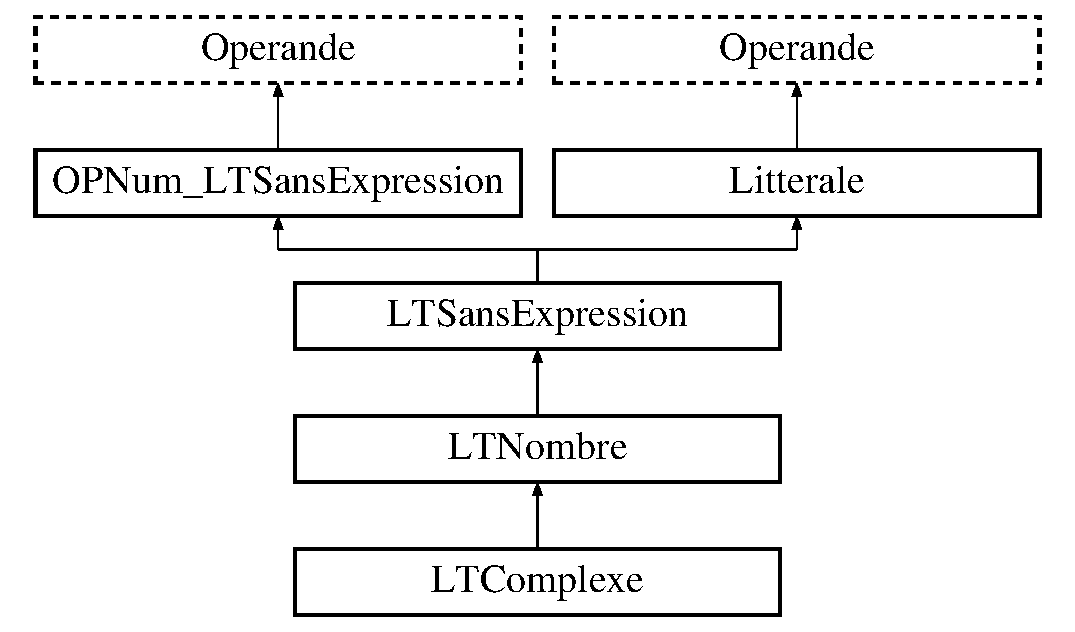
\includegraphics[height=5.000000cm]{class_l_t_complexe}
\end{center}
\end{figure}
\subsection*{Public Member Functions}
\begin{DoxyCompactItemize}
\item 
\hyperlink{class_l_t_complexe_a91582aad82590e2ab764f3aeb9e72c2a}{L\+T\+Complexe} (\hyperlink{class_l_t_numerique}{L\+T\+Numerique} $\ast$r, \hyperlink{class_l_t_numerique}{L\+T\+Numerique} $\ast$i)
\begin{DoxyCompactList}\small\item\em Constructeur. \end{DoxyCompactList}\item 
\hyperlink{class_l_t_complexe_a2faa66c9789d43cc860bc6cda3cb0f2b}{L\+T\+Complexe} (const \hyperlink{class_l_t_complexe}{L\+T\+Complexe} \&c)
\begin{DoxyCompactList}\small\item\em Constructeur par recopie. \end{DoxyCompactList}\item 
virtual \hyperlink{class_l_t_complexe_a124f7db9ebee524023e48035c42ae1c4}{$\sim$\+L\+T\+Complexe} ()\hypertarget{class_l_t_complexe_a124f7db9ebee524023e48035c42ae1c4}{}\label{class_l_t_complexe_a124f7db9ebee524023e48035c42ae1c4}

\begin{DoxyCompactList}\small\item\em Destructeur. \end{DoxyCompactList}\item 
void \hyperlink{class_l_t_complexe_af222794c3f8682060ed0b0cc47f1d2af}{set\+Re} (\hyperlink{class_l_t_numerique}{L\+T\+Numerique} $\ast$v)
\begin{DoxyCompactList}\small\item\em Setter pour la partie réelle. \end{DoxyCompactList}\item 
void \hyperlink{class_l_t_complexe_aa826f44d94f70c341a93d8b0f640a9cd}{set\+Im} (\hyperlink{class_l_t_numerique}{L\+T\+Numerique} $\ast$v)
\begin{DoxyCompactList}\small\item\em Setter pour la partie imaginaire. \end{DoxyCompactList}\item 
\hyperlink{class_l_t_numerique}{L\+T\+Numerique} $\ast$ \hyperlink{class_l_t_complexe_a26dac188af47517274c91ed6884ba324}{get\+Re} () const 
\begin{DoxyCompactList}\small\item\em Getter pour la partie réelle. \end{DoxyCompactList}\item 
\hyperlink{class_l_t_numerique}{L\+T\+Numerique} $\ast$ \hyperlink{class_l_t_complexe_afebf1f447b2d97df62da17ea479e47f3}{get\+Im} () const 
\begin{DoxyCompactList}\small\item\em Getter pour la partie imaginaire. \end{DoxyCompactList}\item 
virtual void \hyperlink{class_l_t_complexe_a5caf7aa1d3123a03294fac536aadf6b1}{afficher} () const \hypertarget{class_l_t_complexe_a5caf7aa1d3123a03294fac536aadf6b1}{}\label{class_l_t_complexe_a5caf7aa1d3123a03294fac536aadf6b1}

\begin{DoxyCompactList}\small\item\em Fonction virtuelle affichant la litterale sur la sortie standart. \end{DoxyCompactList}\item 
virtual Q\+String \hyperlink{class_l_t_complexe_a25992476892bbc3a33ea61dba8bc9160}{get\+Text} () const 
\begin{DoxyCompactList}\small\item\em Fonction virtuelle renvoyant la litterale sous forme de texte. \end{DoxyCompactList}\item 
virtual \hyperlink{class_l_t_complexe}{L\+T\+Complexe} $\ast$ \hyperlink{class_l_t_complexe_ae597257b1e7b81ad6914e44b616c006d}{clone} () const 
\begin{DoxyCompactList}\small\item\em Fonction virtuelle renvoyant une copie de l\textquotesingle{}instance. \end{DoxyCompactList}\item 
virtual \hyperlink{class_l_t_complexe}{L\+T\+Complexe} $\ast$ \hyperlink{class_l_t_complexe_aa4781a2130c4dd2daa81fde8caa6fff3}{simplifier} ()
\begin{DoxyCompactList}\small\item\em Fonction virtuelle simplifiant la litterale actuelle. \end{DoxyCompactList}\item 
virtual \hyperlink{class_l_t_nombre}{L\+T\+Nombre} $\ast$ \hyperlink{class_l_t_complexe_a834cd6715b51f95ad10368fd6e024cdd}{operator+} (\hyperlink{class_l_t_numerique}{L\+T\+Numerique} $\ast$p)
\begin{DoxyCompactList}\small\item\em Addition entre un \hyperlink{class_l_t_complexe}{L\+T\+Complexe} et un \hyperlink{class_l_t_numerique}{L\+T\+Numerique}. \end{DoxyCompactList}\item 
virtual \hyperlink{class_l_t_complexe}{L\+T\+Complexe} $\ast$ \hyperlink{class_l_t_complexe_ac5cb2f0522ce3776b63995047048be3f}{operator+} (\hyperlink{class_l_t_complexe}{L\+T\+Complexe} $\ast$p)
\begin{DoxyCompactList}\small\item\em Addition entre un \hyperlink{class_l_t_complexe}{L\+T\+Complexe} et un \hyperlink{class_l_t_complexe}{L\+T\+Complexe}. \end{DoxyCompactList}\item 
virtual \hyperlink{class_l_t_nombre}{L\+T\+Nombre} $\ast$ \hyperlink{class_l_t_complexe_a201909c43638e4fc38afb660cc3995e6}{operator-\/} (\hyperlink{class_l_t_numerique}{L\+T\+Numerique} $\ast$p)
\begin{DoxyCompactList}\small\item\em Soustraction entre un \hyperlink{class_l_t_complexe}{L\+T\+Complexe} et un \hyperlink{class_l_t_numerique}{L\+T\+Numerique}. \end{DoxyCompactList}\item 
virtual \hyperlink{class_l_t_complexe}{L\+T\+Complexe} $\ast$ \hyperlink{class_l_t_complexe_a15a576fb2400217cf9c0c067c96872f5}{operator-\/} (\hyperlink{class_l_t_complexe}{L\+T\+Complexe} $\ast$p)
\begin{DoxyCompactList}\small\item\em Soustraction entre un \hyperlink{class_l_t_complexe}{L\+T\+Complexe} et un \hyperlink{class_l_t_complexe}{L\+T\+Complexe}. \end{DoxyCompactList}\item 
virtual \hyperlink{class_l_t_nombre}{L\+T\+Nombre} $\ast$ \hyperlink{class_l_t_complexe_a7a03e335c2340d08251b507ef6912a1f}{operator$\ast$} (\hyperlink{class_l_t_numerique}{L\+T\+Numerique} $\ast$p)
\begin{DoxyCompactList}\small\item\em Multiplication entre un \hyperlink{class_l_t_complexe}{L\+T\+Complexe} et un \hyperlink{class_l_t_numerique}{L\+T\+Numerique}. \end{DoxyCompactList}\item 
virtual \hyperlink{class_l_t_complexe}{L\+T\+Complexe} $\ast$ \hyperlink{class_l_t_complexe_a463b0fb6637275a816cfc2ba982e55b6}{operator$\ast$} (\hyperlink{class_l_t_complexe}{L\+T\+Complexe} $\ast$p)
\begin{DoxyCompactList}\small\item\em Multiplication entre un \hyperlink{class_l_t_complexe}{L\+T\+Complexe} et un \hyperlink{class_l_t_complexe}{L\+T\+Complexe}. \end{DoxyCompactList}\item 
virtual \hyperlink{class_l_t_nombre}{L\+T\+Nombre} $\ast$ \hyperlink{class_l_t_complexe_a317bbc9f25b431974a62a7e0950df0f3}{operator/} (\hyperlink{class_l_t_numerique}{L\+T\+Numerique} $\ast$p)
\begin{DoxyCompactList}\small\item\em Division entre un \hyperlink{class_l_t_complexe}{L\+T\+Complexe} et un \hyperlink{class_l_t_numerique}{L\+T\+Numerique}. \end{DoxyCompactList}\item 
virtual \hyperlink{class_l_t_complexe}{L\+T\+Complexe} $\ast$ \hyperlink{class_l_t_complexe_a5b9ab73f38810ee48d4670ae38f48813}{operator/} (\hyperlink{class_l_t_complexe}{L\+T\+Complexe} $\ast$p)
\begin{DoxyCompactList}\small\item\em Division entre un \hyperlink{class_l_t_complexe}{L\+T\+Complexe} et un \hyperlink{class_l_t_numerique}{L\+T\+Numerique}. \end{DoxyCompactList}\end{DoxyCompactItemize}
\subsection*{Friends}
\begin{DoxyCompactItemize}
\item 
bool \hyperlink{class_l_t_complexe_a90de9fd7544467c35afbcb629ee15ef8}{operator==} (\hyperlink{class_l_t_complexe}{L\+T\+Complexe} \&l1, \hyperlink{class_l_t_complexe}{L\+T\+Complexe} \&l2)
\begin{DoxyCompactList}\small\item\em Egalité entre un \hyperlink{class_l_t_complexe}{L\+T\+Complexe} et un \hyperlink{class_l_t_complexe}{L\+T\+Complexe}. \end{DoxyCompactList}\item 
bool \hyperlink{class_l_t_complexe_ab60d8e825b53b8ffdfd42c983314c737}{operator==} (\hyperlink{class_l_t_complexe}{L\+T\+Complexe} \&l1, \hyperlink{class_l_t_numerique}{L\+T\+Numerique} \&l2)
\begin{DoxyCompactList}\small\item\em Egalité entre un \hyperlink{class_l_t_complexe}{L\+T\+Complexe} et un \hyperlink{class_l_t_numerique}{L\+T\+Numerique}. \end{DoxyCompactList}\item 
bool \hyperlink{class_l_t_complexe_a853bdb2627cdac60f907026fef1bfec3}{operator!=} (\hyperlink{class_l_t_complexe}{L\+T\+Complexe} \&l1, \hyperlink{class_l_t_complexe}{L\+T\+Complexe} \&l2)
\begin{DoxyCompactList}\small\item\em Différence entre un \hyperlink{class_l_t_complexe}{L\+T\+Complexe} et un \hyperlink{class_l_t_complexe}{L\+T\+Complexe}. \end{DoxyCompactList}\item 
bool \hyperlink{class_l_t_complexe_a0c157bab9d494f8c817fe550ec5279d1}{operator!=} (\hyperlink{class_l_t_complexe}{L\+T\+Complexe} \&l1, \hyperlink{class_l_t_numerique}{L\+T\+Numerique} \&l2)
\begin{DoxyCompactList}\small\item\em Différence entre un \hyperlink{class_l_t_complexe}{L\+T\+Complexe} et un \hyperlink{class_l_t_numerique}{L\+T\+Numerique}. \end{DoxyCompactList}\end{DoxyCompactItemize}


\subsection{Detailed Description}
Classe gérant les nombres complexes. 

\subsection{Constructor \& Destructor Documentation}
\index{L\+T\+Complexe@{L\+T\+Complexe}!L\+T\+Complexe@{L\+T\+Complexe}}
\index{L\+T\+Complexe@{L\+T\+Complexe}!L\+T\+Complexe@{L\+T\+Complexe}}
\subsubsection[{\texorpdfstring{L\+T\+Complexe(\+L\+T\+Numerique $\ast$r, L\+T\+Numerique $\ast$i)}{LTComplexe(LTNumerique *r, LTNumerique *i)}}]{\setlength{\rightskip}{0pt plus 5cm}L\+T\+Complexe\+::\+L\+T\+Complexe (
\begin{DoxyParamCaption}
\item[{{\bf L\+T\+Numerique} $\ast$}]{r, }
\item[{{\bf L\+T\+Numerique} $\ast$}]{i}
\end{DoxyParamCaption}
)\hspace{0.3cm}{\ttfamily [inline]}}\hypertarget{class_l_t_complexe_a91582aad82590e2ab764f3aeb9e72c2a}{}\label{class_l_t_complexe_a91582aad82590e2ab764f3aeb9e72c2a}


Constructeur. 


\begin{DoxyParams}{Parameters}
{\em r} & Partie réelle \\
\hline
{\em i} & Partie imaginaire \\
\hline
\end{DoxyParams}
\index{L\+T\+Complexe@{L\+T\+Complexe}!L\+T\+Complexe@{L\+T\+Complexe}}
\index{L\+T\+Complexe@{L\+T\+Complexe}!L\+T\+Complexe@{L\+T\+Complexe}}
\subsubsection[{\texorpdfstring{L\+T\+Complexe(const L\+T\+Complexe \&c)}{LTComplexe(const LTComplexe &c)}}]{\setlength{\rightskip}{0pt plus 5cm}L\+T\+Complexe\+::\+L\+T\+Complexe (
\begin{DoxyParamCaption}
\item[{const {\bf L\+T\+Complexe} \&}]{c}
\end{DoxyParamCaption}
)\hspace{0.3cm}{\ttfamily [inline]}}\hypertarget{class_l_t_complexe_a2faa66c9789d43cc860bc6cda3cb0f2b}{}\label{class_l_t_complexe_a2faa66c9789d43cc860bc6cda3cb0f2b}


Constructeur par recopie. 


\begin{DoxyParams}{Parameters}
{\em c} & Complexe \\
\hline
\end{DoxyParams}


\subsection{Member Function Documentation}
\index{L\+T\+Complexe@{L\+T\+Complexe}!clone@{clone}}
\index{clone@{clone}!L\+T\+Complexe@{L\+T\+Complexe}}
\subsubsection[{\texorpdfstring{clone() const }{clone() const }}]{\setlength{\rightskip}{0pt plus 5cm}{\bf L\+T\+Complexe} $\ast$ L\+T\+Complexe\+::clone (
\begin{DoxyParamCaption}
{}
\end{DoxyParamCaption}
) const\hspace{0.3cm}{\ttfamily [virtual]}}\hypertarget{class_l_t_complexe_ae597257b1e7b81ad6914e44b616c006d}{}\label{class_l_t_complexe_ae597257b1e7b81ad6914e44b616c006d}


Fonction virtuelle renvoyant une copie de l\textquotesingle{}instance. 

\begin{DoxyReturn}{Returns}
Nouvelle litterale copiée 
\end{DoxyReturn}


Implements \hyperlink{class_l_t_nombre_a09ad6faddbb007746e41af6873bd1824}{L\+T\+Nombre}.

\index{L\+T\+Complexe@{L\+T\+Complexe}!get\+Im@{get\+Im}}
\index{get\+Im@{get\+Im}!L\+T\+Complexe@{L\+T\+Complexe}}
\subsubsection[{\texorpdfstring{get\+Im() const }{getIm() const }}]{\setlength{\rightskip}{0pt plus 5cm}{\bf L\+T\+Numerique}$\ast$ L\+T\+Complexe\+::get\+Im (
\begin{DoxyParamCaption}
{}
\end{DoxyParamCaption}
) const\hspace{0.3cm}{\ttfamily [inline]}}\hypertarget{class_l_t_complexe_afebf1f447b2d97df62da17ea479e47f3}{}\label{class_l_t_complexe_afebf1f447b2d97df62da17ea479e47f3}


Getter pour la partie imaginaire. 

\begin{DoxyReturn}{Returns}
\hyperlink{class_litterale}{Litterale} numérique représentant la partie imaginaire 
\end{DoxyReturn}
\index{L\+T\+Complexe@{L\+T\+Complexe}!get\+Re@{get\+Re}}
\index{get\+Re@{get\+Re}!L\+T\+Complexe@{L\+T\+Complexe}}
\subsubsection[{\texorpdfstring{get\+Re() const }{getRe() const }}]{\setlength{\rightskip}{0pt plus 5cm}{\bf L\+T\+Numerique}$\ast$ L\+T\+Complexe\+::get\+Re (
\begin{DoxyParamCaption}
{}
\end{DoxyParamCaption}
) const\hspace{0.3cm}{\ttfamily [inline]}}\hypertarget{class_l_t_complexe_a26dac188af47517274c91ed6884ba324}{}\label{class_l_t_complexe_a26dac188af47517274c91ed6884ba324}


Getter pour la partie réelle. 

\begin{DoxyReturn}{Returns}
\hyperlink{class_litterale}{Litterale} numérique représentant la partie réelle 
\end{DoxyReturn}
\index{L\+T\+Complexe@{L\+T\+Complexe}!get\+Text@{get\+Text}}
\index{get\+Text@{get\+Text}!L\+T\+Complexe@{L\+T\+Complexe}}
\subsubsection[{\texorpdfstring{get\+Text() const }{getText() const }}]{\setlength{\rightskip}{0pt plus 5cm}Q\+String L\+T\+Complexe\+::get\+Text (
\begin{DoxyParamCaption}
{}
\end{DoxyParamCaption}
) const\hspace{0.3cm}{\ttfamily [virtual]}}\hypertarget{class_l_t_complexe_a25992476892bbc3a33ea61dba8bc9160}{}\label{class_l_t_complexe_a25992476892bbc3a33ea61dba8bc9160}


Fonction virtuelle renvoyant la litterale sous forme de texte. 

\begin{DoxyReturn}{Returns}
\hyperlink{class_litterale}{Litterale} sous forme de texte 
\end{DoxyReturn}


Implements \hyperlink{class_l_t_nombre_a39fe941ec69bf013bc3be8b3e575c3d0}{L\+T\+Nombre}.

\index{L\+T\+Complexe@{L\+T\+Complexe}!operator$\ast$@{operator$\ast$}}
\index{operator$\ast$@{operator$\ast$}!L\+T\+Complexe@{L\+T\+Complexe}}
\subsubsection[{\texorpdfstring{operator$\ast$(\+L\+T\+Numerique $\ast$p)}{operator*(LTNumerique *p)}}]{\setlength{\rightskip}{0pt plus 5cm}{\bf L\+T\+Nombre} $\ast$ L\+T\+Complexe\+::operator$\ast$ (
\begin{DoxyParamCaption}
\item[{{\bf L\+T\+Numerique} $\ast$}]{p}
\end{DoxyParamCaption}
)\hspace{0.3cm}{\ttfamily [virtual]}}\hypertarget{class_l_t_complexe_a7a03e335c2340d08251b507ef6912a1f}{}\label{class_l_t_complexe_a7a03e335c2340d08251b507ef6912a1f}


Multiplication entre un \hyperlink{class_l_t_complexe}{L\+T\+Complexe} et un \hyperlink{class_l_t_numerique}{L\+T\+Numerique}. 


\begin{DoxyParams}{Parameters}
{\em p} & Variable à ajouter \\
\hline
\end{DoxyParams}
\begin{DoxyReturn}{Returns}
\hyperlink{class_l_t_nombre}{L\+T\+Nombre} créé 
\end{DoxyReturn}


Implements \hyperlink{class_l_t_nombre_af77bf71cb71f2409ee78ae8421958bfe}{L\+T\+Nombre}.

\index{L\+T\+Complexe@{L\+T\+Complexe}!operator$\ast$@{operator$\ast$}}
\index{operator$\ast$@{operator$\ast$}!L\+T\+Complexe@{L\+T\+Complexe}}
\subsubsection[{\texorpdfstring{operator$\ast$(\+L\+T\+Complexe $\ast$p)}{operator*(LTComplexe *p)}}]{\setlength{\rightskip}{0pt plus 5cm}{\bf L\+T\+Complexe} $\ast$ L\+T\+Complexe\+::operator$\ast$ (
\begin{DoxyParamCaption}
\item[{{\bf L\+T\+Complexe} $\ast$}]{p}
\end{DoxyParamCaption}
)\hspace{0.3cm}{\ttfamily [virtual]}}\hypertarget{class_l_t_complexe_a463b0fb6637275a816cfc2ba982e55b6}{}\label{class_l_t_complexe_a463b0fb6637275a816cfc2ba982e55b6}


Multiplication entre un \hyperlink{class_l_t_complexe}{L\+T\+Complexe} et un \hyperlink{class_l_t_complexe}{L\+T\+Complexe}. 


\begin{DoxyParams}{Parameters}
{\em p} & Variable à ajouter \\
\hline
\end{DoxyParams}
\begin{DoxyReturn}{Returns}
\hyperlink{class_l_t_complexe}{L\+T\+Complexe} créé 
\end{DoxyReturn}


Implements \hyperlink{class_l_t_nombre_a90743859f0a4197a698d44be68d5c47b}{L\+T\+Nombre}.

\index{L\+T\+Complexe@{L\+T\+Complexe}!operator+@{operator+}}
\index{operator+@{operator+}!L\+T\+Complexe@{L\+T\+Complexe}}
\subsubsection[{\texorpdfstring{operator+(\+L\+T\+Numerique $\ast$p)}{operator+(LTNumerique *p)}}]{\setlength{\rightskip}{0pt plus 5cm}{\bf L\+T\+Nombre} $\ast$ L\+T\+Complexe\+::operator+ (
\begin{DoxyParamCaption}
\item[{{\bf L\+T\+Numerique} $\ast$}]{p}
\end{DoxyParamCaption}
)\hspace{0.3cm}{\ttfamily [virtual]}}\hypertarget{class_l_t_complexe_a834cd6715b51f95ad10368fd6e024cdd}{}\label{class_l_t_complexe_a834cd6715b51f95ad10368fd6e024cdd}


Addition entre un \hyperlink{class_l_t_complexe}{L\+T\+Complexe} et un \hyperlink{class_l_t_numerique}{L\+T\+Numerique}. 


\begin{DoxyParams}{Parameters}
{\em p} & Variable à ajouter \\
\hline
\end{DoxyParams}
\begin{DoxyReturn}{Returns}
\hyperlink{class_l_t_nombre}{L\+T\+Nombre} créé 
\end{DoxyReturn}


Implements \hyperlink{class_l_t_nombre_a3962ef35dcfd735800ed5630e55a1d81}{L\+T\+Nombre}.

\index{L\+T\+Complexe@{L\+T\+Complexe}!operator+@{operator+}}
\index{operator+@{operator+}!L\+T\+Complexe@{L\+T\+Complexe}}
\subsubsection[{\texorpdfstring{operator+(\+L\+T\+Complexe $\ast$p)}{operator+(LTComplexe *p)}}]{\setlength{\rightskip}{0pt plus 5cm}{\bf L\+T\+Complexe} $\ast$ L\+T\+Complexe\+::operator+ (
\begin{DoxyParamCaption}
\item[{{\bf L\+T\+Complexe} $\ast$}]{p}
\end{DoxyParamCaption}
)\hspace{0.3cm}{\ttfamily [virtual]}}\hypertarget{class_l_t_complexe_ac5cb2f0522ce3776b63995047048be3f}{}\label{class_l_t_complexe_ac5cb2f0522ce3776b63995047048be3f}


Addition entre un \hyperlink{class_l_t_complexe}{L\+T\+Complexe} et un \hyperlink{class_l_t_complexe}{L\+T\+Complexe}. 


\begin{DoxyParams}{Parameters}
{\em p} & Variable à ajouter \\
\hline
\end{DoxyParams}
\begin{DoxyReturn}{Returns}
\hyperlink{class_l_t_complexe}{L\+T\+Complexe} créé 
\end{DoxyReturn}


Implements \hyperlink{class_l_t_nombre_a8caa60dd6bf935dc68e8a37bd527b4d8}{L\+T\+Nombre}.

\index{L\+T\+Complexe@{L\+T\+Complexe}!operator-\/@{operator-\/}}
\index{operator-\/@{operator-\/}!L\+T\+Complexe@{L\+T\+Complexe}}
\subsubsection[{\texorpdfstring{operator-\/(\+L\+T\+Numerique $\ast$p)}{operator-(LTNumerique *p)}}]{\setlength{\rightskip}{0pt plus 5cm}{\bf L\+T\+Nombre} $\ast$ L\+T\+Complexe\+::operator-\/ (
\begin{DoxyParamCaption}
\item[{{\bf L\+T\+Numerique} $\ast$}]{p}
\end{DoxyParamCaption}
)\hspace{0.3cm}{\ttfamily [virtual]}}\hypertarget{class_l_t_complexe_a201909c43638e4fc38afb660cc3995e6}{}\label{class_l_t_complexe_a201909c43638e4fc38afb660cc3995e6}


Soustraction entre un \hyperlink{class_l_t_complexe}{L\+T\+Complexe} et un \hyperlink{class_l_t_numerique}{L\+T\+Numerique}. 


\begin{DoxyParams}{Parameters}
{\em p} & Variable à ajouter \\
\hline
\end{DoxyParams}
\begin{DoxyReturn}{Returns}
\hyperlink{class_l_t_nombre}{L\+T\+Nombre} créé 
\end{DoxyReturn}


Implements \hyperlink{class_l_t_nombre_ade4345e2555976c45c433fcc6d91e417}{L\+T\+Nombre}.

\index{L\+T\+Complexe@{L\+T\+Complexe}!operator-\/@{operator-\/}}
\index{operator-\/@{operator-\/}!L\+T\+Complexe@{L\+T\+Complexe}}
\subsubsection[{\texorpdfstring{operator-\/(\+L\+T\+Complexe $\ast$p)}{operator-(LTComplexe *p)}}]{\setlength{\rightskip}{0pt plus 5cm}{\bf L\+T\+Complexe} $\ast$ L\+T\+Complexe\+::operator-\/ (
\begin{DoxyParamCaption}
\item[{{\bf L\+T\+Complexe} $\ast$}]{p}
\end{DoxyParamCaption}
)\hspace{0.3cm}{\ttfamily [virtual]}}\hypertarget{class_l_t_complexe_a15a576fb2400217cf9c0c067c96872f5}{}\label{class_l_t_complexe_a15a576fb2400217cf9c0c067c96872f5}


Soustraction entre un \hyperlink{class_l_t_complexe}{L\+T\+Complexe} et un \hyperlink{class_l_t_complexe}{L\+T\+Complexe}. 


\begin{DoxyParams}{Parameters}
{\em p} & Variable à ajouter \\
\hline
\end{DoxyParams}
\begin{DoxyReturn}{Returns}
\hyperlink{class_l_t_complexe}{L\+T\+Complexe} créé 
\end{DoxyReturn}


Implements \hyperlink{class_l_t_nombre_a60d335475d7b623f6f8ff513494e6572}{L\+T\+Nombre}.

\index{L\+T\+Complexe@{L\+T\+Complexe}!operator/@{operator/}}
\index{operator/@{operator/}!L\+T\+Complexe@{L\+T\+Complexe}}
\subsubsection[{\texorpdfstring{operator/(\+L\+T\+Numerique $\ast$p)}{operator/(LTNumerique *p)}}]{\setlength{\rightskip}{0pt plus 5cm}{\bf L\+T\+Nombre} $\ast$ L\+T\+Complexe\+::operator/ (
\begin{DoxyParamCaption}
\item[{{\bf L\+T\+Numerique} $\ast$}]{p}
\end{DoxyParamCaption}
)\hspace{0.3cm}{\ttfamily [virtual]}}\hypertarget{class_l_t_complexe_a317bbc9f25b431974a62a7e0950df0f3}{}\label{class_l_t_complexe_a317bbc9f25b431974a62a7e0950df0f3}


Division entre un \hyperlink{class_l_t_complexe}{L\+T\+Complexe} et un \hyperlink{class_l_t_numerique}{L\+T\+Numerique}. 


\begin{DoxyParams}{Parameters}
{\em p} & Variable à ajouter \\
\hline
\end{DoxyParams}
\begin{DoxyReturn}{Returns}
\hyperlink{class_l_t_nombre}{L\+T\+Nombre} créé 
\end{DoxyReturn}


Implements \hyperlink{class_l_t_nombre_abfb3b0f925a6706222173779cf3f762d}{L\+T\+Nombre}.

\index{L\+T\+Complexe@{L\+T\+Complexe}!operator/@{operator/}}
\index{operator/@{operator/}!L\+T\+Complexe@{L\+T\+Complexe}}
\subsubsection[{\texorpdfstring{operator/(\+L\+T\+Complexe $\ast$p)}{operator/(LTComplexe *p)}}]{\setlength{\rightskip}{0pt plus 5cm}{\bf L\+T\+Complexe} $\ast$ L\+T\+Complexe\+::operator/ (
\begin{DoxyParamCaption}
\item[{{\bf L\+T\+Complexe} $\ast$}]{p}
\end{DoxyParamCaption}
)\hspace{0.3cm}{\ttfamily [virtual]}}\hypertarget{class_l_t_complexe_a5b9ab73f38810ee48d4670ae38f48813}{}\label{class_l_t_complexe_a5b9ab73f38810ee48d4670ae38f48813}


Division entre un \hyperlink{class_l_t_complexe}{L\+T\+Complexe} et un \hyperlink{class_l_t_numerique}{L\+T\+Numerique}. 


\begin{DoxyParams}{Parameters}
{\em p} & Variable à ajouter \\
\hline
\end{DoxyParams}
\begin{DoxyReturn}{Returns}
\hyperlink{class_l_t_complexe}{L\+T\+Complexe} créé 
\end{DoxyReturn}


Implements \hyperlink{class_l_t_nombre_ae7e0f2dba7aba0f3251e18c5cfc60b5a}{L\+T\+Nombre}.

\index{L\+T\+Complexe@{L\+T\+Complexe}!set\+Im@{set\+Im}}
\index{set\+Im@{set\+Im}!L\+T\+Complexe@{L\+T\+Complexe}}
\subsubsection[{\texorpdfstring{set\+Im(\+L\+T\+Numerique $\ast$v)}{setIm(LTNumerique *v)}}]{\setlength{\rightskip}{0pt plus 5cm}void L\+T\+Complexe\+::set\+Im (
\begin{DoxyParamCaption}
\item[{{\bf L\+T\+Numerique} $\ast$}]{v}
\end{DoxyParamCaption}
)\hspace{0.3cm}{\ttfamily [inline]}}\hypertarget{class_l_t_complexe_aa826f44d94f70c341a93d8b0f640a9cd}{}\label{class_l_t_complexe_aa826f44d94f70c341a93d8b0f640a9cd}


Setter pour la partie imaginaire. 


\begin{DoxyParams}{Parameters}
{\em v} & \hyperlink{class_l_t_numerique}{L\+T\+Numerique} représentation la partie imaginaire \\
\hline
\end{DoxyParams}
\index{L\+T\+Complexe@{L\+T\+Complexe}!set\+Re@{set\+Re}}
\index{set\+Re@{set\+Re}!L\+T\+Complexe@{L\+T\+Complexe}}
\subsubsection[{\texorpdfstring{set\+Re(\+L\+T\+Numerique $\ast$v)}{setRe(LTNumerique *v)}}]{\setlength{\rightskip}{0pt plus 5cm}void L\+T\+Complexe\+::set\+Re (
\begin{DoxyParamCaption}
\item[{{\bf L\+T\+Numerique} $\ast$}]{v}
\end{DoxyParamCaption}
)\hspace{0.3cm}{\ttfamily [inline]}}\hypertarget{class_l_t_complexe_af222794c3f8682060ed0b0cc47f1d2af}{}\label{class_l_t_complexe_af222794c3f8682060ed0b0cc47f1d2af}


Setter pour la partie réelle. 


\begin{DoxyParams}{Parameters}
{\em v} & \hyperlink{class_l_t_numerique}{L\+T\+Numerique} représentation la partie réeelle \\
\hline
\end{DoxyParams}
\index{L\+T\+Complexe@{L\+T\+Complexe}!simplifier@{simplifier}}
\index{simplifier@{simplifier}!L\+T\+Complexe@{L\+T\+Complexe}}
\subsubsection[{\texorpdfstring{simplifier()}{simplifier()}}]{\setlength{\rightskip}{0pt plus 5cm}virtual {\bf L\+T\+Complexe}$\ast$ L\+T\+Complexe\+::simplifier (
\begin{DoxyParamCaption}
{}
\end{DoxyParamCaption}
)\hspace{0.3cm}{\ttfamily [inline]}, {\ttfamily [virtual]}}\hypertarget{class_l_t_complexe_aa4781a2130c4dd2daa81fde8caa6fff3}{}\label{class_l_t_complexe_aa4781a2130c4dd2daa81fde8caa6fff3}


Fonction virtuelle simplifiant la litterale actuelle. 

\begin{DoxyReturn}{Returns}
Nouvelle litterale copiée 
\end{DoxyReturn}


Implements \hyperlink{class_l_t_nombre_a6aa1593c8c0956bb5412bfee3c15b085}{L\+T\+Nombre}.



\subsection{Friends And Related Function Documentation}
\index{L\+T\+Complexe@{L\+T\+Complexe}!operator"!=@{operator"!=}}
\index{operator"!=@{operator"!=}!L\+T\+Complexe@{L\+T\+Complexe}}
\subsubsection[{\texorpdfstring{operator"!=}{operator!=}}]{\setlength{\rightskip}{0pt plus 5cm}bool operator!= (
\begin{DoxyParamCaption}
\item[{{\bf L\+T\+Complexe} \&}]{l1, }
\item[{{\bf L\+T\+Complexe} \&}]{l2}
\end{DoxyParamCaption}
)\hspace{0.3cm}{\ttfamily [friend]}}\hypertarget{class_l_t_complexe_a853bdb2627cdac60f907026fef1bfec3}{}\label{class_l_t_complexe_a853bdb2627cdac60f907026fef1bfec3}


Différence entre un \hyperlink{class_l_t_complexe}{L\+T\+Complexe} et un \hyperlink{class_l_t_complexe}{L\+T\+Complexe}. 


\begin{DoxyParams}{Parameters}
{\em l1} & Premier paramètre, qui sera modifié \\
\hline
{\em l2} & Second paramètre qui sera ajouté au premier \\
\hline
\end{DoxyParams}
\begin{DoxyReturn}{Returns}
Booléen de confirmation pour la création 
\end{DoxyReturn}
\index{L\+T\+Complexe@{L\+T\+Complexe}!operator"!=@{operator"!=}}
\index{operator"!=@{operator"!=}!L\+T\+Complexe@{L\+T\+Complexe}}
\subsubsection[{\texorpdfstring{operator"!=}{operator!=}}]{\setlength{\rightskip}{0pt plus 5cm}bool operator!= (
\begin{DoxyParamCaption}
\item[{{\bf L\+T\+Complexe} \&}]{l1, }
\item[{{\bf L\+T\+Numerique} \&}]{l2}
\end{DoxyParamCaption}
)\hspace{0.3cm}{\ttfamily [friend]}}\hypertarget{class_l_t_complexe_a0c157bab9d494f8c817fe550ec5279d1}{}\label{class_l_t_complexe_a0c157bab9d494f8c817fe550ec5279d1}


Différence entre un \hyperlink{class_l_t_complexe}{L\+T\+Complexe} et un \hyperlink{class_l_t_numerique}{L\+T\+Numerique}. 


\begin{DoxyParams}{Parameters}
{\em l1} & Premier paramètre, qui sera modifié \\
\hline
{\em l2} & Second paramètre qui sera ajouté au premier \\
\hline
\end{DoxyParams}
\begin{DoxyReturn}{Returns}
Booléen de confirmation pour la création 
\end{DoxyReturn}
\index{L\+T\+Complexe@{L\+T\+Complexe}!operator==@{operator==}}
\index{operator==@{operator==}!L\+T\+Complexe@{L\+T\+Complexe}}
\subsubsection[{\texorpdfstring{operator==}{operator==}}]{\setlength{\rightskip}{0pt plus 5cm}bool operator== (
\begin{DoxyParamCaption}
\item[{{\bf L\+T\+Complexe} \&}]{l1, }
\item[{{\bf L\+T\+Complexe} \&}]{l2}
\end{DoxyParamCaption}
)\hspace{0.3cm}{\ttfamily [friend]}}\hypertarget{class_l_t_complexe_a90de9fd7544467c35afbcb629ee15ef8}{}\label{class_l_t_complexe_a90de9fd7544467c35afbcb629ee15ef8}


Egalité entre un \hyperlink{class_l_t_complexe}{L\+T\+Complexe} et un \hyperlink{class_l_t_complexe}{L\+T\+Complexe}. 


\begin{DoxyParams}{Parameters}
{\em l1} & Premier paramètre, qui sera modifié \\
\hline
{\em l2} & Second paramètre qui sera ajouté au premier \\
\hline
\end{DoxyParams}
\begin{DoxyReturn}{Returns}
Booléen de confirmation pour la création 
\end{DoxyReturn}
\index{L\+T\+Complexe@{L\+T\+Complexe}!operator==@{operator==}}
\index{operator==@{operator==}!L\+T\+Complexe@{L\+T\+Complexe}}
\subsubsection[{\texorpdfstring{operator==}{operator==}}]{\setlength{\rightskip}{0pt plus 5cm}bool operator== (
\begin{DoxyParamCaption}
\item[{{\bf L\+T\+Complexe} \&}]{l1, }
\item[{{\bf L\+T\+Numerique} \&}]{l2}
\end{DoxyParamCaption}
)\hspace{0.3cm}{\ttfamily [friend]}}\hypertarget{class_l_t_complexe_ab60d8e825b53b8ffdfd42c983314c737}{}\label{class_l_t_complexe_ab60d8e825b53b8ffdfd42c983314c737}


Egalité entre un \hyperlink{class_l_t_complexe}{L\+T\+Complexe} et un \hyperlink{class_l_t_numerique}{L\+T\+Numerique}. 


\begin{DoxyParams}{Parameters}
{\em l1} & Premier paramètre, qui sera modifié \\
\hline
{\em l2} & Second paramètre qui sera ajouté au premier \\
\hline
\end{DoxyParams}
\begin{DoxyReturn}{Returns}
Booléen de confirmation pour la création 
\end{DoxyReturn}


The documentation for this class was generated from the following files\+:\begin{DoxyCompactItemize}
\item 
ltcomplexe.\+h\item 
ltcomplexe.\+cpp\end{DoxyCompactItemize}

\hypertarget{class_l_t_entier}{}\section{L\+T\+Entier Class Reference}
\label{class_l_t_entier}\index{L\+T\+Entier@{L\+T\+Entier}}
Inheritance diagram for L\+T\+Entier\+:\begin{figure}[H]
\begin{center}
\leavevmode
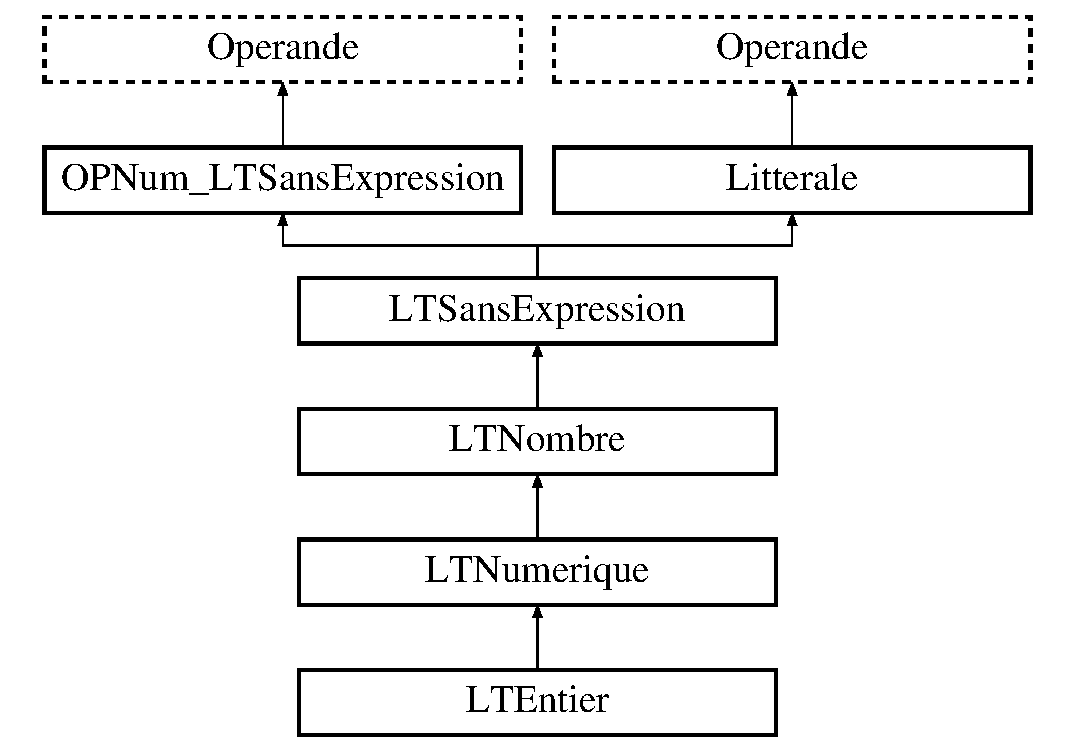
\includegraphics[height=6.000000cm]{class_l_t_entier}
\end{center}
\end{figure}
\subsection*{Public Member Functions}
\begin{DoxyCompactItemize}
\item 
{\bfseries L\+T\+Entier} (int v, \hyperlink{class_l_t_atome}{L\+T\+Atome} $\ast$a=0)\hypertarget{class_l_t_entier_a5966d1f1fc4f16d154135681e5b51bd7}{}\label{class_l_t_entier_a5966d1f1fc4f16d154135681e5b51bd7}

\item 
{\bfseries L\+T\+Entier} (Q\+String v, \hyperlink{class_l_t_atome}{L\+T\+Atome} $\ast$a=0)\hypertarget{class_l_t_entier_a3cefeb71a20650403cfbd91b243550ff}{}\label{class_l_t_entier_a3cefeb71a20650403cfbd91b243550ff}

\item 
{\bfseries L\+T\+Entier} (const \hyperlink{class_l_t_entier}{L\+T\+Entier} \&e, \hyperlink{class_l_t_atome}{L\+T\+Atome} $\ast$a=0)\hypertarget{class_l_t_entier_ab91a13030b55f961a4630869e154501d}{}\label{class_l_t_entier_ab91a13030b55f961a4630869e154501d}

\item 
int {\bfseries get\+Value} () const \hypertarget{class_l_t_entier_a1b34875fe8312a408b221967a9ea9863}{}\label{class_l_t_entier_a1b34875fe8312a408b221967a9ea9863}

\item 
void {\bfseries set\+Value} (int v)\hypertarget{class_l_t_entier_acfd0a6e53763fa7b0dc003e76b21d123}{}\label{class_l_t_entier_acfd0a6e53763fa7b0dc003e76b21d123}

\item 
void {\bfseries set\+Value} (Q\+String v)\hypertarget{class_l_t_entier_a647928737573ef6077e60c5e05052347}{}\label{class_l_t_entier_a647928737573ef6077e60c5e05052347}

\item 
virtual void \hyperlink{class_l_t_entier_a00b3854cd7ac676cbf3f0f8ff698da73}{afficher} () const \hypertarget{class_l_t_entier_a00b3854cd7ac676cbf3f0f8ff698da73}{}\label{class_l_t_entier_a00b3854cd7ac676cbf3f0f8ff698da73}

\begin{DoxyCompactList}\small\item\em Fonction virtuelle affichant la litterale sur la sortie standart. \end{DoxyCompactList}\item 
virtual Q\+String \hyperlink{class_l_t_entier_a735c05de25b1264a5b2bc603f63eed58}{get\+Text} () const 
\begin{DoxyCompactList}\small\item\em Fonction virtuelle renvoyant la litterale sous forme de texte. \end{DoxyCompactList}\item 
virtual \hyperlink{class_l_t_entier}{L\+T\+Entier} $\ast$ \hyperlink{class_l_t_entier_afc21b025efd3feea0162053902b8d640}{clone} () const 
\begin{DoxyCompactList}\small\item\em Fonction virtuelle renvoyant une copie de l\textquotesingle{}instance. \end{DoxyCompactList}\item 
virtual \hyperlink{class_l_t_entier}{L\+T\+Entier} $\ast$ \hyperlink{class_l_t_entier_a3dd0959762240ef5cbe0a62970728ddf}{simplifier} ()
\begin{DoxyCompactList}\small\item\em Fonction virtuelle simplifiant la litterale actuelle. \end{DoxyCompactList}\item 
virtual \hyperlink{class_l_t_entier}{L\+T\+Entier} $\ast$ {\bfseries operator-\/-\/} ()\hypertarget{class_l_t_entier_a6bae152bbfed3d8035ad1aa03d9202a7}{}\label{class_l_t_entier_a6bae152bbfed3d8035ad1aa03d9202a7}

\item 
virtual \hyperlink{class_l_t_numerique}{L\+T\+Numerique} $\ast$ \hyperlink{class_l_t_entier_ab61b9d54516e57b37923433cbb76ced7}{operator+} (\hyperlink{class_l_t_numerique}{L\+T\+Numerique} $\ast$p)
\begin{DoxyCompactList}\small\item\em Addition entre un \hyperlink{class_l_t_complexe}{L\+T\+Complexe} et un \hyperlink{class_l_t_numerique}{L\+T\+Numerique}. \end{DoxyCompactList}\item 
virtual \hyperlink{class_l_t_complexe}{L\+T\+Complexe} $\ast$ \hyperlink{class_l_t_entier_af87e5527f3e09fa388313b880ba92c84}{operator+} (\hyperlink{class_l_t_complexe}{L\+T\+Complexe} $\ast$p)
\begin{DoxyCompactList}\small\item\em Addition entre un \hyperlink{class_l_t_complexe}{L\+T\+Complexe} et un \hyperlink{class_l_t_complexe}{L\+T\+Complexe}. \end{DoxyCompactList}\item 
virtual \hyperlink{class_l_t_numerique}{L\+T\+Numerique} $\ast$ \hyperlink{class_l_t_entier_ae7d462d020affefeb6a348ae17ce8c95}{operator-\/} (\hyperlink{class_l_t_numerique}{L\+T\+Numerique} $\ast$p)
\begin{DoxyCompactList}\small\item\em Soustraction entre un \hyperlink{class_l_t_complexe}{L\+T\+Complexe} et un \hyperlink{class_l_t_numerique}{L\+T\+Numerique}. \end{DoxyCompactList}\item 
virtual \hyperlink{class_l_t_complexe}{L\+T\+Complexe} $\ast$ \hyperlink{class_l_t_entier_a2fa9e6e1f2cdcdfb3fc5cd85985928e6}{operator-\/} (\hyperlink{class_l_t_complexe}{L\+T\+Complexe} $\ast$p)
\begin{DoxyCompactList}\small\item\em Soustraction entre un \hyperlink{class_l_t_complexe}{L\+T\+Complexe} et un \hyperlink{class_l_t_complexe}{L\+T\+Complexe}. \end{DoxyCompactList}\item 
virtual \hyperlink{class_l_t_numerique}{L\+T\+Numerique} $\ast$ \hyperlink{class_l_t_entier_a77d0c8047664798243c81017c6402612}{operator$\ast$} (\hyperlink{class_l_t_numerique}{L\+T\+Numerique} $\ast$p)
\begin{DoxyCompactList}\small\item\em Multiplication entre un \hyperlink{class_l_t_complexe}{L\+T\+Complexe} et un \hyperlink{class_l_t_numerique}{L\+T\+Numerique}. \end{DoxyCompactList}\item 
virtual \hyperlink{class_l_t_complexe}{L\+T\+Complexe} $\ast$ \hyperlink{class_l_t_entier_a621d0a41b4347cd02f0c99052b9f8e55}{operator$\ast$} (\hyperlink{class_l_t_complexe}{L\+T\+Complexe} $\ast$p)
\begin{DoxyCompactList}\small\item\em Multiplication entre un \hyperlink{class_l_t_complexe}{L\+T\+Complexe} et un \hyperlink{class_l_t_complexe}{L\+T\+Complexe}. \end{DoxyCompactList}\item 
virtual \hyperlink{class_l_t_numerique}{L\+T\+Numerique} $\ast$ \hyperlink{class_l_t_entier_abde7f75a9aec4852f4f624cf94080fdc}{operator/} (\hyperlink{class_l_t_numerique}{L\+T\+Numerique} $\ast$p)
\begin{DoxyCompactList}\small\item\em Division entre un \hyperlink{class_l_t_complexe}{L\+T\+Complexe} et un \hyperlink{class_l_t_numerique}{L\+T\+Numerique}. \end{DoxyCompactList}\item 
virtual \hyperlink{class_l_t_complexe}{L\+T\+Complexe} $\ast$ \hyperlink{class_l_t_entier_a59f046d2849150eba46ffbc1edcf6b95}{operator/} (\hyperlink{class_l_t_complexe}{L\+T\+Complexe} $\ast$p)
\begin{DoxyCompactList}\small\item\em Division entre un \hyperlink{class_l_t_complexe}{L\+T\+Complexe} et un \hyperlink{class_l_t_numerique}{L\+T\+Numerique}. \end{DoxyCompactList}\item 
virtual bool {\bfseries operator\&\&} (\hyperlink{class_l_t_entier}{L\+T\+Entier} $\ast$p) const \hypertarget{class_l_t_entier_a4ce3ced22f60210d8a4fb5186103164f}{}\label{class_l_t_entier_a4ce3ced22f60210d8a4fb5186103164f}

\item 
virtual bool {\bfseries operator$\vert$$\vert$} (\hyperlink{class_l_t_entier}{L\+T\+Entier} $\ast$p) const \hypertarget{class_l_t_entier_a6e7dd1aaac5aa6fa4fd882619fb90712}{}\label{class_l_t_entier_a6e7dd1aaac5aa6fa4fd882619fb90712}

\item 
virtual bool {\bfseries operator!} () const \hypertarget{class_l_t_entier_ad97f456d3ae1c6d755894760c29d85e8}{}\label{class_l_t_entier_ad97f456d3ae1c6d755894760c29d85e8}

\end{DoxyCompactItemize}
\subsection*{Static Public Attributes}
\begin{DoxyCompactItemize}
\item 
static const \hyperlink{class_l_t_entier}{L\+T\+Entier} {\bfseries zero} = \hyperlink{class_l_t_entier}{L\+T\+Entier}(0)\hypertarget{class_l_t_entier_a6b3afa86731df2551f829e4ece67bb8f}{}\label{class_l_t_entier_a6b3afa86731df2551f829e4ece67bb8f}

\end{DoxyCompactItemize}
\subsection*{Friends}
\begin{DoxyCompactItemize}
\item 
bool {\bfseries operator==} (\hyperlink{class_l_t_entier}{L\+T\+Entier} \&l1, \hyperlink{class_l_t_entier}{L\+T\+Entier} \&l2)\hypertarget{class_l_t_entier_ad3e747bb85c29afb0bee5df6121b7b0b}{}\label{class_l_t_entier_ad3e747bb85c29afb0bee5df6121b7b0b}

\item 
bool {\bfseries operator==} (\hyperlink{class_l_t_entier}{L\+T\+Entier} \&l1, \hyperlink{class_l_t_reelle}{L\+T\+Reelle} \&l2)\hypertarget{class_l_t_entier_a833d4722d91b3ff8a42c2955622ff4df}{}\label{class_l_t_entier_a833d4722d91b3ff8a42c2955622ff4df}

\item 
bool {\bfseries operator==} (\hyperlink{class_l_t_entier}{L\+T\+Entier} \&l1, \hyperlink{class_l_t_rationnelle}{L\+T\+Rationnelle} \&l2)\hypertarget{class_l_t_entier_a17c0f48909de6fd8d119ed9e756568ed}{}\label{class_l_t_entier_a17c0f48909de6fd8d119ed9e756568ed}

\item 
bool {\bfseries operator$<$} (\hyperlink{class_l_t_entier}{L\+T\+Entier} \&l1, \hyperlink{class_l_t_entier}{L\+T\+Entier} \&l2)\hypertarget{class_l_t_entier_a2e81bf35692e93c53388aa79f173665b}{}\label{class_l_t_entier_a2e81bf35692e93c53388aa79f173665b}

\item 
bool {\bfseries operator$<$} (\hyperlink{class_l_t_entier}{L\+T\+Entier} \&l1, \hyperlink{class_l_t_reelle}{L\+T\+Reelle} \&l2)\hypertarget{class_l_t_entier_af662380021aa46205cf4552096204671}{}\label{class_l_t_entier_af662380021aa46205cf4552096204671}

\item 
bool {\bfseries operator$<$} (\hyperlink{class_l_t_entier}{L\+T\+Entier} \&l1, \hyperlink{class_l_t_rationnelle}{L\+T\+Rationnelle} \&l2)\hypertarget{class_l_t_entier_ae0e9d295db8a3d7e2bed1b8b09b4a596}{}\label{class_l_t_entier_ae0e9d295db8a3d7e2bed1b8b09b4a596}

\end{DoxyCompactItemize}
\subsection*{Additional Inherited Members}


\subsection{Member Function Documentation}
\index{L\+T\+Entier@{L\+T\+Entier}!clone@{clone}}
\index{clone@{clone}!L\+T\+Entier@{L\+T\+Entier}}
\subsubsection[{\texorpdfstring{clone() const }{clone() const }}]{\setlength{\rightskip}{0pt plus 5cm}{\bf L\+T\+Entier} $\ast$ L\+T\+Entier\+::clone (
\begin{DoxyParamCaption}
{}
\end{DoxyParamCaption}
) const\hspace{0.3cm}{\ttfamily [virtual]}}\hypertarget{class_l_t_entier_afc21b025efd3feea0162053902b8d640}{}\label{class_l_t_entier_afc21b025efd3feea0162053902b8d640}


Fonction virtuelle renvoyant une copie de l\textquotesingle{}instance. 

\begin{DoxyReturn}{Returns}
Nouvelle litterale copiée 
\end{DoxyReturn}


Implements \hyperlink{class_l_t_numerique_a884056443dd30cd71c49b42b5ba63581}{L\+T\+Numerique}.

\index{L\+T\+Entier@{L\+T\+Entier}!get\+Text@{get\+Text}}
\index{get\+Text@{get\+Text}!L\+T\+Entier@{L\+T\+Entier}}
\subsubsection[{\texorpdfstring{get\+Text() const }{getText() const }}]{\setlength{\rightskip}{0pt plus 5cm}Q\+String L\+T\+Entier\+::get\+Text (
\begin{DoxyParamCaption}
{}
\end{DoxyParamCaption}
) const\hspace{0.3cm}{\ttfamily [virtual]}}\hypertarget{class_l_t_entier_a735c05de25b1264a5b2bc603f63eed58}{}\label{class_l_t_entier_a735c05de25b1264a5b2bc603f63eed58}


Fonction virtuelle renvoyant la litterale sous forme de texte. 

\begin{DoxyReturn}{Returns}
\hyperlink{class_litterale}{Litterale} sous forme de texte 
\end{DoxyReturn}


Implements \hyperlink{class_l_t_numerique_abef28b1b62ee356717f70f4317a44590}{L\+T\+Numerique}.

\index{L\+T\+Entier@{L\+T\+Entier}!operator$\ast$@{operator$\ast$}}
\index{operator$\ast$@{operator$\ast$}!L\+T\+Entier@{L\+T\+Entier}}
\subsubsection[{\texorpdfstring{operator$\ast$(\+L\+T\+Numerique $\ast$p)}{operator*(LTNumerique *p)}}]{\setlength{\rightskip}{0pt plus 5cm}{\bf L\+T\+Numerique} $\ast$ L\+T\+Entier\+::operator$\ast$ (
\begin{DoxyParamCaption}
\item[{{\bf L\+T\+Numerique} $\ast$}]{p}
\end{DoxyParamCaption}
)\hspace{0.3cm}{\ttfamily [virtual]}}\hypertarget{class_l_t_entier_a77d0c8047664798243c81017c6402612}{}\label{class_l_t_entier_a77d0c8047664798243c81017c6402612}


Multiplication entre un \hyperlink{class_l_t_complexe}{L\+T\+Complexe} et un \hyperlink{class_l_t_numerique}{L\+T\+Numerique}. 


\begin{DoxyParams}{Parameters}
{\em p} & Variable à ajouter \\
\hline
\end{DoxyParams}
\begin{DoxyReturn}{Returns}
\hyperlink{class_l_t_nombre}{L\+T\+Nombre} créé 
\end{DoxyReturn}


Implements \hyperlink{class_l_t_numerique_aef374b7679c6b9b7901e0a4bbfce4cc3}{L\+T\+Numerique}.

\index{L\+T\+Entier@{L\+T\+Entier}!operator$\ast$@{operator$\ast$}}
\index{operator$\ast$@{operator$\ast$}!L\+T\+Entier@{L\+T\+Entier}}
\subsubsection[{\texorpdfstring{operator$\ast$(\+L\+T\+Complexe $\ast$p)}{operator*(LTComplexe *p)}}]{\setlength{\rightskip}{0pt plus 5cm}{\bf L\+T\+Complexe} $\ast$ L\+T\+Entier\+::operator$\ast$ (
\begin{DoxyParamCaption}
\item[{{\bf L\+T\+Complexe} $\ast$}]{p}
\end{DoxyParamCaption}
)\hspace{0.3cm}{\ttfamily [virtual]}}\hypertarget{class_l_t_entier_a621d0a41b4347cd02f0c99052b9f8e55}{}\label{class_l_t_entier_a621d0a41b4347cd02f0c99052b9f8e55}


Multiplication entre un \hyperlink{class_l_t_complexe}{L\+T\+Complexe} et un \hyperlink{class_l_t_complexe}{L\+T\+Complexe}. 


\begin{DoxyParams}{Parameters}
{\em p} & Variable à ajouter \\
\hline
\end{DoxyParams}
\begin{DoxyReturn}{Returns}
\hyperlink{class_l_t_complexe}{L\+T\+Complexe} créé 
\end{DoxyReturn}


Implements \hyperlink{class_l_t_numerique_a6991c6c854915c7bfd98634c791ab815}{L\+T\+Numerique}.

\index{L\+T\+Entier@{L\+T\+Entier}!operator+@{operator+}}
\index{operator+@{operator+}!L\+T\+Entier@{L\+T\+Entier}}
\subsubsection[{\texorpdfstring{operator+(\+L\+T\+Numerique $\ast$p)}{operator+(LTNumerique *p)}}]{\setlength{\rightskip}{0pt plus 5cm}{\bf L\+T\+Numerique} $\ast$ L\+T\+Entier\+::operator+ (
\begin{DoxyParamCaption}
\item[{{\bf L\+T\+Numerique} $\ast$}]{p}
\end{DoxyParamCaption}
)\hspace{0.3cm}{\ttfamily [virtual]}}\hypertarget{class_l_t_entier_ab61b9d54516e57b37923433cbb76ced7}{}\label{class_l_t_entier_ab61b9d54516e57b37923433cbb76ced7}


Addition entre un \hyperlink{class_l_t_complexe}{L\+T\+Complexe} et un \hyperlink{class_l_t_numerique}{L\+T\+Numerique}. 


\begin{DoxyParams}{Parameters}
{\em p} & Variable à ajouter \\
\hline
\end{DoxyParams}
\begin{DoxyReturn}{Returns}
\hyperlink{class_l_t_nombre}{L\+T\+Nombre} créé 
\end{DoxyReturn}


Implements \hyperlink{class_l_t_numerique_a9fb09223dc517fae452f4af0d50f6966}{L\+T\+Numerique}.

\index{L\+T\+Entier@{L\+T\+Entier}!operator+@{operator+}}
\index{operator+@{operator+}!L\+T\+Entier@{L\+T\+Entier}}
\subsubsection[{\texorpdfstring{operator+(\+L\+T\+Complexe $\ast$p)}{operator+(LTComplexe *p)}}]{\setlength{\rightskip}{0pt plus 5cm}{\bf L\+T\+Complexe} $\ast$ L\+T\+Entier\+::operator+ (
\begin{DoxyParamCaption}
\item[{{\bf L\+T\+Complexe} $\ast$}]{p}
\end{DoxyParamCaption}
)\hspace{0.3cm}{\ttfamily [virtual]}}\hypertarget{class_l_t_entier_af87e5527f3e09fa388313b880ba92c84}{}\label{class_l_t_entier_af87e5527f3e09fa388313b880ba92c84}


Addition entre un \hyperlink{class_l_t_complexe}{L\+T\+Complexe} et un \hyperlink{class_l_t_complexe}{L\+T\+Complexe}. 


\begin{DoxyParams}{Parameters}
{\em p} & Variable à ajouter \\
\hline
\end{DoxyParams}
\begin{DoxyReturn}{Returns}
\hyperlink{class_l_t_complexe}{L\+T\+Complexe} créé 
\end{DoxyReturn}


Implements \hyperlink{class_l_t_numerique_a615173a7cd77e649235d1c06d72726e7}{L\+T\+Numerique}.

\index{L\+T\+Entier@{L\+T\+Entier}!operator-\/@{operator-\/}}
\index{operator-\/@{operator-\/}!L\+T\+Entier@{L\+T\+Entier}}
\subsubsection[{\texorpdfstring{operator-\/(\+L\+T\+Numerique $\ast$p)}{operator-(LTNumerique *p)}}]{\setlength{\rightskip}{0pt plus 5cm}{\bf L\+T\+Numerique} $\ast$ L\+T\+Entier\+::operator-\/ (
\begin{DoxyParamCaption}
\item[{{\bf L\+T\+Numerique} $\ast$}]{p}
\end{DoxyParamCaption}
)\hspace{0.3cm}{\ttfamily [virtual]}}\hypertarget{class_l_t_entier_ae7d462d020affefeb6a348ae17ce8c95}{}\label{class_l_t_entier_ae7d462d020affefeb6a348ae17ce8c95}


Soustraction entre un \hyperlink{class_l_t_complexe}{L\+T\+Complexe} et un \hyperlink{class_l_t_numerique}{L\+T\+Numerique}. 


\begin{DoxyParams}{Parameters}
{\em p} & Variable à ajouter \\
\hline
\end{DoxyParams}
\begin{DoxyReturn}{Returns}
\hyperlink{class_l_t_nombre}{L\+T\+Nombre} créé 
\end{DoxyReturn}


Implements \hyperlink{class_l_t_numerique_a94d98eef8d391bdb925dbb70a1b35834}{L\+T\+Numerique}.

\index{L\+T\+Entier@{L\+T\+Entier}!operator-\/@{operator-\/}}
\index{operator-\/@{operator-\/}!L\+T\+Entier@{L\+T\+Entier}}
\subsubsection[{\texorpdfstring{operator-\/(\+L\+T\+Complexe $\ast$p)}{operator-(LTComplexe *p)}}]{\setlength{\rightskip}{0pt plus 5cm}{\bf L\+T\+Complexe} $\ast$ L\+T\+Entier\+::operator-\/ (
\begin{DoxyParamCaption}
\item[{{\bf L\+T\+Complexe} $\ast$}]{p}
\end{DoxyParamCaption}
)\hspace{0.3cm}{\ttfamily [virtual]}}\hypertarget{class_l_t_entier_a2fa9e6e1f2cdcdfb3fc5cd85985928e6}{}\label{class_l_t_entier_a2fa9e6e1f2cdcdfb3fc5cd85985928e6}


Soustraction entre un \hyperlink{class_l_t_complexe}{L\+T\+Complexe} et un \hyperlink{class_l_t_complexe}{L\+T\+Complexe}. 


\begin{DoxyParams}{Parameters}
{\em p} & Variable à ajouter \\
\hline
\end{DoxyParams}
\begin{DoxyReturn}{Returns}
\hyperlink{class_l_t_complexe}{L\+T\+Complexe} créé 
\end{DoxyReturn}


Implements \hyperlink{class_l_t_numerique_a45bbf62a5725c3b9c8a8a14d9be6ef47}{L\+T\+Numerique}.

\index{L\+T\+Entier@{L\+T\+Entier}!operator/@{operator/}}
\index{operator/@{operator/}!L\+T\+Entier@{L\+T\+Entier}}
\subsubsection[{\texorpdfstring{operator/(\+L\+T\+Numerique $\ast$p)}{operator/(LTNumerique *p)}}]{\setlength{\rightskip}{0pt plus 5cm}{\bf L\+T\+Numerique} $\ast$ L\+T\+Entier\+::operator/ (
\begin{DoxyParamCaption}
\item[{{\bf L\+T\+Numerique} $\ast$}]{p}
\end{DoxyParamCaption}
)\hspace{0.3cm}{\ttfamily [virtual]}}\hypertarget{class_l_t_entier_abde7f75a9aec4852f4f624cf94080fdc}{}\label{class_l_t_entier_abde7f75a9aec4852f4f624cf94080fdc}


Division entre un \hyperlink{class_l_t_complexe}{L\+T\+Complexe} et un \hyperlink{class_l_t_numerique}{L\+T\+Numerique}. 


\begin{DoxyParams}{Parameters}
{\em p} & Variable à ajouter \\
\hline
\end{DoxyParams}
\begin{DoxyReturn}{Returns}
\hyperlink{class_l_t_nombre}{L\+T\+Nombre} créé 
\end{DoxyReturn}


Implements \hyperlink{class_l_t_numerique_ab3acc500e7c92b2d1e05ebc65561b84a}{L\+T\+Numerique}.

\index{L\+T\+Entier@{L\+T\+Entier}!operator/@{operator/}}
\index{operator/@{operator/}!L\+T\+Entier@{L\+T\+Entier}}
\subsubsection[{\texorpdfstring{operator/(\+L\+T\+Complexe $\ast$p)}{operator/(LTComplexe *p)}}]{\setlength{\rightskip}{0pt plus 5cm}{\bf L\+T\+Complexe} $\ast$ L\+T\+Entier\+::operator/ (
\begin{DoxyParamCaption}
\item[{{\bf L\+T\+Complexe} $\ast$}]{p}
\end{DoxyParamCaption}
)\hspace{0.3cm}{\ttfamily [virtual]}}\hypertarget{class_l_t_entier_a59f046d2849150eba46ffbc1edcf6b95}{}\label{class_l_t_entier_a59f046d2849150eba46ffbc1edcf6b95}


Division entre un \hyperlink{class_l_t_complexe}{L\+T\+Complexe} et un \hyperlink{class_l_t_numerique}{L\+T\+Numerique}. 


\begin{DoxyParams}{Parameters}
{\em p} & Variable à ajouter \\
\hline
\end{DoxyParams}
\begin{DoxyReturn}{Returns}
\hyperlink{class_l_t_complexe}{L\+T\+Complexe} créé 
\end{DoxyReturn}


Implements \hyperlink{class_l_t_numerique_a223402e5b15e25f716bdd1981f59f39d}{L\+T\+Numerique}.

\index{L\+T\+Entier@{L\+T\+Entier}!simplifier@{simplifier}}
\index{simplifier@{simplifier}!L\+T\+Entier@{L\+T\+Entier}}
\subsubsection[{\texorpdfstring{simplifier()}{simplifier()}}]{\setlength{\rightskip}{0pt plus 5cm}virtual {\bf L\+T\+Entier}$\ast$ L\+T\+Entier\+::simplifier (
\begin{DoxyParamCaption}
{}
\end{DoxyParamCaption}
)\hspace{0.3cm}{\ttfamily [inline]}, {\ttfamily [virtual]}}\hypertarget{class_l_t_entier_a3dd0959762240ef5cbe0a62970728ddf}{}\label{class_l_t_entier_a3dd0959762240ef5cbe0a62970728ddf}


Fonction virtuelle simplifiant la litterale actuelle. 

\begin{DoxyReturn}{Returns}
Nouvelle litterale copiée 
\end{DoxyReturn}


Implements \hyperlink{class_l_t_numerique_a3963de62916188d01f93b1d0fdb42c7f}{L\+T\+Numerique}.



The documentation for this class was generated from the following files\+:\begin{DoxyCompactItemize}
\item 
ltnumerique.\+h\item 
ltnumerique.\+cpp\end{DoxyCompactItemize}

\hypertarget{class_l_t_expression}{}\section{L\+T\+Expression Class Reference}
\label{class_l_t_expression}\index{L\+T\+Expression@{L\+T\+Expression}}


Classe \hyperlink{class_l_t_expression}{L\+T\+Expression}, gérant les expressions.  




{\ttfamily \#include $<$ltexpression.\+h$>$}

Inheritance diagram for L\+T\+Expression\+:\begin{figure}[H]
\begin{center}
\leavevmode
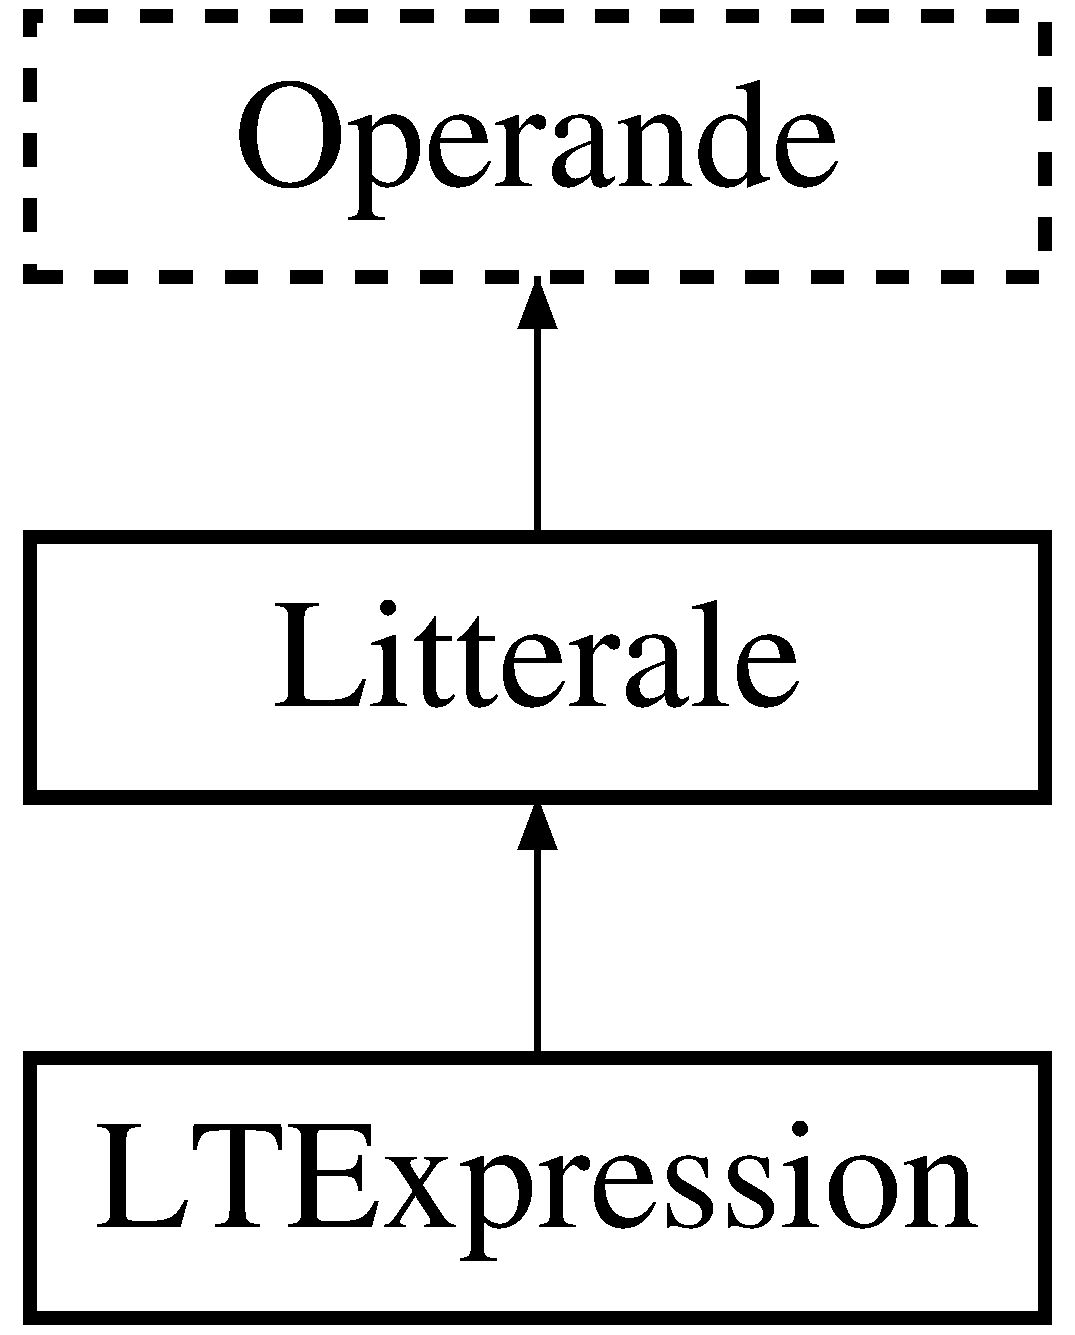
\includegraphics[height=3.000000cm]{class_l_t_expression}
\end{center}
\end{figure}
\subsection*{Public Member Functions}
\begin{DoxyCompactItemize}
\item 
\hyperlink{class_l_t_expression_a61fdf50726f54c3ecdea78150859aab3}{L\+T\+Expression} (\hyperlink{class_l_t_atome}{L\+T\+Atome} $\ast$id, Q\+List$<$ \hyperlink{class_o_p_num___l_t_sans_expression}{O\+P\+Num\+\_\+\+L\+T\+Sans\+Expression} $\ast$ $>$ l)
\begin{DoxyCompactList}\small\item\em Constructeur. \end{DoxyCompactList}\item 
\hyperlink{class_l_t_expression_a92e9b49739f4d707544ed6f816409189}{L\+T\+Expression} (Q\+List$<$ \hyperlink{class_o_p_num___l_t_sans_expression}{O\+P\+Num\+\_\+\+L\+T\+Sans\+Expression} $\ast$ $>$ l)
\begin{DoxyCompactList}\small\item\em Constructeur. \end{DoxyCompactList}\item 
virtual \hyperlink{class_l_t_expression_aa8530b38f8f14319e9b0c2d90f75511d}{$\sim$\+L\+T\+Expression} ()\hypertarget{class_l_t_expression_aa8530b38f8f14319e9b0c2d90f75511d}{}\label{class_l_t_expression_aa8530b38f8f14319e9b0c2d90f75511d}

\begin{DoxyCompactList}\small\item\em Destructeur. \end{DoxyCompactList}\item 
virtual Q\+String \hyperlink{class_l_t_expression_acb3e72d9d7c2beaa2e1349eb1f9bec18}{get\+Content\+To\+Compute} () const 
\begin{DoxyCompactList}\small\item\em Fonction qui renvoie une string de l\textquotesingle{}expression. \end{DoxyCompactList}\item 
Q\+List$<$ \hyperlink{class_o_p_num___l_t_sans_expression}{O\+P\+Num\+\_\+\+L\+T\+Sans\+Expression} $\ast$ $>$ \hyperlink{class_l_t_expression_ad42d9dc5ab8990110e9e9b956401d1b9}{get\+List} ()
\begin{DoxyCompactList}\small\item\em Fonction qui renvoie la liste du contenu de l\textquotesingle{}expression. \end{DoxyCompactList}\item 
virtual void \hyperlink{class_l_t_expression_a5d222890ba90f2e0a3674f5c2f32b94b}{afficher} () const \hypertarget{class_l_t_expression_a5d222890ba90f2e0a3674f5c2f32b94b}{}\label{class_l_t_expression_a5d222890ba90f2e0a3674f5c2f32b94b}

\begin{DoxyCompactList}\small\item\em Fonction virtuelle affichant la litterale sur la sortie standart. \end{DoxyCompactList}\item 
virtual Q\+String \hyperlink{class_l_t_expression_a13d5a9d4a536ed34effcb08a6e5391a6}{get\+Text} () const 
\begin{DoxyCompactList}\small\item\em Fonction virtuelle renvoyant la litterale sous forme de texte. \end{DoxyCompactList}\item 
virtual \hyperlink{class_l_t_expression}{L\+T\+Expression} $\ast$ \hyperlink{class_l_t_expression_ab51c526b6232a131bea9a43945633b2a}{clone} () const 
\begin{DoxyCompactList}\small\item\em Fonction virtuelle renvoyant une copie de l\textquotesingle{}instance. \end{DoxyCompactList}\item 
virtual \hyperlink{class_l_t_expression}{L\+T\+Expression} $\ast$ \hyperlink{class_l_t_expression_a8817e6f26189ad7a4e65bd24f6020367}{simplifier} ()
\begin{DoxyCompactList}\small\item\em Fonction virtuelle simplifiant la litterale actuelle. \end{DoxyCompactList}\item 
virtual \hyperlink{class_l_t_expression}{L\+T\+Expression} $\ast$ \hyperlink{class_l_t_expression_a10eaec4e530a4e763daa16f919d40d8a}{concatener} (\hyperlink{class_l_t_expression}{L\+T\+Expression} $\ast$E2, Q\+String op)
\begin{DoxyCompactList}\small\item\em Fonction qui concatenne un opérateur à la fin d\textquotesingle{}une expression. \end{DoxyCompactList}\end{DoxyCompactItemize}


\subsection{Detailed Description}
Classe \hyperlink{class_l_t_expression}{L\+T\+Expression}, gérant les expressions. 

\subsection{Constructor \& Destructor Documentation}
\index{L\+T\+Expression@{L\+T\+Expression}!L\+T\+Expression@{L\+T\+Expression}}
\index{L\+T\+Expression@{L\+T\+Expression}!L\+T\+Expression@{L\+T\+Expression}}
\subsubsection[{\texorpdfstring{L\+T\+Expression(\+L\+T\+Atome $\ast$id, Q\+List$<$ O\+P\+Num\+\_\+\+L\+T\+Sans\+Expression $\ast$ $>$ l)}{LTExpression(LTAtome *id, QList< OPNum_LTSansExpression * > l)}}]{\setlength{\rightskip}{0pt plus 5cm}L\+T\+Expression\+::\+L\+T\+Expression (
\begin{DoxyParamCaption}
\item[{{\bf L\+T\+Atome} $\ast$}]{id, }
\item[{Q\+List$<$ {\bf O\+P\+Num\+\_\+\+L\+T\+Sans\+Expression} $\ast$ $>$}]{l}
\end{DoxyParamCaption}
)\hspace{0.3cm}{\ttfamily [inline]}}\hypertarget{class_l_t_expression_a61fdf50726f54c3ecdea78150859aab3}{}\label{class_l_t_expression_a61fdf50726f54c3ecdea78150859aab3}


Constructeur. 


\begin{DoxyParams}{Parameters}
{\em id} & Atome identifiant l\textquotesingle{}expression \\
\hline
{\em l} & Contenu de l\textquotesingle{}expression \\
\hline
\end{DoxyParams}
\index{L\+T\+Expression@{L\+T\+Expression}!L\+T\+Expression@{L\+T\+Expression}}
\index{L\+T\+Expression@{L\+T\+Expression}!L\+T\+Expression@{L\+T\+Expression}}
\subsubsection[{\texorpdfstring{L\+T\+Expression(\+Q\+List$<$ O\+P\+Num\+\_\+\+L\+T\+Sans\+Expression $\ast$ $>$ l)}{LTExpression(QList< OPNum_LTSansExpression * > l)}}]{\setlength{\rightskip}{0pt plus 5cm}L\+T\+Expression\+::\+L\+T\+Expression (
\begin{DoxyParamCaption}
\item[{Q\+List$<$ {\bf O\+P\+Num\+\_\+\+L\+T\+Sans\+Expression} $\ast$ $>$}]{l}
\end{DoxyParamCaption}
)\hspace{0.3cm}{\ttfamily [inline]}}\hypertarget{class_l_t_expression_a92e9b49739f4d707544ed6f816409189}{}\label{class_l_t_expression_a92e9b49739f4d707544ed6f816409189}


Constructeur. 


\begin{DoxyParams}{Parameters}
{\em l} & Contenu de l\textquotesingle{}expression \\
\hline
\end{DoxyParams}


\subsection{Member Function Documentation}
\index{L\+T\+Expression@{L\+T\+Expression}!clone@{clone}}
\index{clone@{clone}!L\+T\+Expression@{L\+T\+Expression}}
\subsubsection[{\texorpdfstring{clone() const }{clone() const }}]{\setlength{\rightskip}{0pt plus 5cm}virtual {\bf L\+T\+Expression}$\ast$ L\+T\+Expression\+::clone (
\begin{DoxyParamCaption}
{}
\end{DoxyParamCaption}
) const\hspace{0.3cm}{\ttfamily [inline]}, {\ttfamily [virtual]}}\hypertarget{class_l_t_expression_ab51c526b6232a131bea9a43945633b2a}{}\label{class_l_t_expression_ab51c526b6232a131bea9a43945633b2a}


Fonction virtuelle renvoyant une copie de l\textquotesingle{}instance. 

\begin{DoxyReturn}{Returns}
Nouvelle litterale copiée 
\end{DoxyReturn}


Implements \hyperlink{class_litterale_a08967178d22c3d69e6c3e86ea8c85888}{Litterale}.

\index{L\+T\+Expression@{L\+T\+Expression}!concatener@{concatener}}
\index{concatener@{concatener}!L\+T\+Expression@{L\+T\+Expression}}
\subsubsection[{\texorpdfstring{concatener(\+L\+T\+Expression $\ast$\+E2, Q\+String op)}{concatener(LTExpression *E2, QString op)}}]{\setlength{\rightskip}{0pt plus 5cm}virtual {\bf L\+T\+Expression}$\ast$ L\+T\+Expression\+::concatener (
\begin{DoxyParamCaption}
\item[{{\bf L\+T\+Expression} $\ast$}]{E2, }
\item[{Q\+String}]{op}
\end{DoxyParamCaption}
)\hspace{0.3cm}{\ttfamily [inline]}, {\ttfamily [virtual]}}\hypertarget{class_l_t_expression_a10eaec4e530a4e763daa16f919d40d8a}{}\label{class_l_t_expression_a10eaec4e530a4e763daa16f919d40d8a}


Fonction qui concatenne un opérateur à la fin d\textquotesingle{}une expression. 


\begin{DoxyParams}{Parameters}
{\em E2} & Expression \\
\hline
{\em op} & Opérateur \\
\hline
\end{DoxyParams}
\begin{DoxyReturn}{Returns}
Expression 
\end{DoxyReturn}
\index{L\+T\+Expression@{L\+T\+Expression}!get\+Content\+To\+Compute@{get\+Content\+To\+Compute}}
\index{get\+Content\+To\+Compute@{get\+Content\+To\+Compute}!L\+T\+Expression@{L\+T\+Expression}}
\subsubsection[{\texorpdfstring{get\+Content\+To\+Compute() const }{getContentToCompute() const }}]{\setlength{\rightskip}{0pt plus 5cm}virtual Q\+String L\+T\+Expression\+::get\+Content\+To\+Compute (
\begin{DoxyParamCaption}
{}
\end{DoxyParamCaption}
) const\hspace{0.3cm}{\ttfamily [inline]}, {\ttfamily [virtual]}}\hypertarget{class_l_t_expression_acb3e72d9d7c2beaa2e1349eb1f9bec18}{}\label{class_l_t_expression_acb3e72d9d7c2beaa2e1349eb1f9bec18}


Fonction qui renvoie une string de l\textquotesingle{}expression. 

\begin{DoxyReturn}{Returns}
Texte de l\textquotesingle{}expression 
\end{DoxyReturn}
\index{L\+T\+Expression@{L\+T\+Expression}!get\+List@{get\+List}}
\index{get\+List@{get\+List}!L\+T\+Expression@{L\+T\+Expression}}
\subsubsection[{\texorpdfstring{get\+List()}{getList()}}]{\setlength{\rightskip}{0pt plus 5cm}Q\+List$<${\bf O\+P\+Num\+\_\+\+L\+T\+Sans\+Expression}$\ast$$>$ L\+T\+Expression\+::get\+List (
\begin{DoxyParamCaption}
{}
\end{DoxyParamCaption}
)\hspace{0.3cm}{\ttfamily [inline]}}\hypertarget{class_l_t_expression_ad42d9dc5ab8990110e9e9b956401d1b9}{}\label{class_l_t_expression_ad42d9dc5ab8990110e9e9b956401d1b9}


Fonction qui renvoie la liste du contenu de l\textquotesingle{}expression. 

\begin{DoxyReturn}{Returns}
Texte de l\textquotesingle{}expression 
\end{DoxyReturn}
\index{L\+T\+Expression@{L\+T\+Expression}!get\+Text@{get\+Text}}
\index{get\+Text@{get\+Text}!L\+T\+Expression@{L\+T\+Expression}}
\subsubsection[{\texorpdfstring{get\+Text() const }{getText() const }}]{\setlength{\rightskip}{0pt plus 5cm}virtual Q\+String L\+T\+Expression\+::get\+Text (
\begin{DoxyParamCaption}
{}
\end{DoxyParamCaption}
) const\hspace{0.3cm}{\ttfamily [inline]}, {\ttfamily [virtual]}}\hypertarget{class_l_t_expression_a13d5a9d4a536ed34effcb08a6e5391a6}{}\label{class_l_t_expression_a13d5a9d4a536ed34effcb08a6e5391a6}


Fonction virtuelle renvoyant la litterale sous forme de texte. 

\begin{DoxyReturn}{Returns}
\hyperlink{class_litterale}{Litterale} sous forme de texte 
\end{DoxyReturn}


Implements \hyperlink{class_litterale_a780075c00abf31efb87e7c28843ea029}{Litterale}.

\index{L\+T\+Expression@{L\+T\+Expression}!simplifier@{simplifier}}
\index{simplifier@{simplifier}!L\+T\+Expression@{L\+T\+Expression}}
\subsubsection[{\texorpdfstring{simplifier()}{simplifier()}}]{\setlength{\rightskip}{0pt plus 5cm}virtual {\bf L\+T\+Expression}$\ast$ L\+T\+Expression\+::simplifier (
\begin{DoxyParamCaption}
{}
\end{DoxyParamCaption}
)\hspace{0.3cm}{\ttfamily [inline]}, {\ttfamily [virtual]}}\hypertarget{class_l_t_expression_a8817e6f26189ad7a4e65bd24f6020367}{}\label{class_l_t_expression_a8817e6f26189ad7a4e65bd24f6020367}


Fonction virtuelle simplifiant la litterale actuelle. 

\begin{DoxyReturn}{Returns}
Nouvelle litterale copiée 
\end{DoxyReturn}


Implements \hyperlink{class_litterale_af33a0c1a4a9a5bb687da112b12f0e6e6}{Litterale}.



The documentation for this class was generated from the following file\+:\begin{DoxyCompactItemize}
\item 
ltexpression.\+h\end{DoxyCompactItemize}

\hypertarget{class_l_t_nombre}{}\section{L\+T\+Nombre Class Reference}
\label{class_l_t_nombre}\index{L\+T\+Nombre@{L\+T\+Nombre}}


Classe \hyperlink{class_l_t_nombre}{L\+T\+Nombre} abstraite.  




{\ttfamily \#include $<$ltnombre.\+h$>$}

Inheritance diagram for L\+T\+Nombre\+:\begin{figure}[H]
\begin{center}
\leavevmode
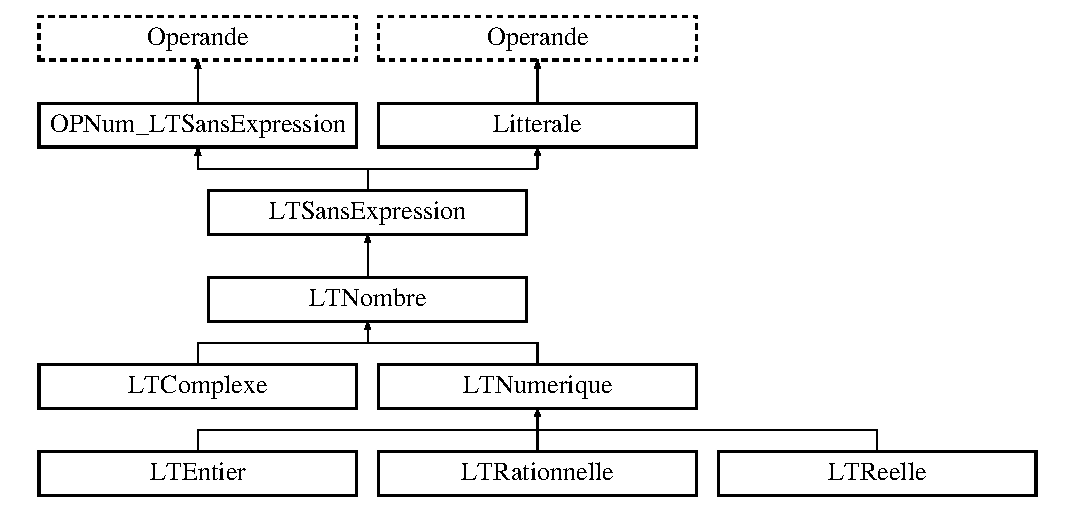
\includegraphics[height=6.000000cm]{class_l_t_nombre}
\end{center}
\end{figure}
\subsection*{Public Member Functions}
\begin{DoxyCompactItemize}
\item 
\hyperlink{class_l_t_nombre_ae1651d09e64312a910569e0bd6cc4408}{L\+T\+Nombre} ()\hypertarget{class_l_t_nombre_ae1651d09e64312a910569e0bd6cc4408}{}\label{class_l_t_nombre_ae1651d09e64312a910569e0bd6cc4408}

\begin{DoxyCompactList}\small\item\em Constructeur. \end{DoxyCompactList}\item 
virtual \hyperlink{class_l_t_nombre_ad12b52a30fda647436512754199ab135}{$\sim$\+L\+T\+Nombre} ()\hypertarget{class_l_t_nombre_ad12b52a30fda647436512754199ab135}{}\label{class_l_t_nombre_ad12b52a30fda647436512754199ab135}

\begin{DoxyCompactList}\small\item\em Destructeur. \end{DoxyCompactList}\item 
virtual Q\+String \hyperlink{class_l_t_nombre_a39fe941ec69bf013bc3be8b3e575c3d0}{get\+Text} () const  =0
\begin{DoxyCompactList}\small\item\em Fonction virtuelle renvoyant la litterale sous forme de texte. \end{DoxyCompactList}\item 
virtual void \hyperlink{class_l_t_nombre_aa06e186ee3ded2189e1a98a68d913775}{afficher} () const  =0\hypertarget{class_l_t_nombre_aa06e186ee3ded2189e1a98a68d913775}{}\label{class_l_t_nombre_aa06e186ee3ded2189e1a98a68d913775}

\begin{DoxyCompactList}\small\item\em Fonction virtuelle affichant la litterale sur la sortie standart. \end{DoxyCompactList}\item 
virtual \hyperlink{class_l_t_nombre}{L\+T\+Nombre} $\ast$ \hyperlink{class_l_t_nombre_a09ad6faddbb007746e41af6873bd1824}{clone} () const  =0
\begin{DoxyCompactList}\small\item\em Fonction virtuelle renvoyant une copie de l\textquotesingle{}instance. \end{DoxyCompactList}\item 
virtual \hyperlink{class_l_t_nombre}{L\+T\+Nombre} $\ast$ \hyperlink{class_l_t_nombre_a6aa1593c8c0956bb5412bfee3c15b085}{simplifier} ()=0
\begin{DoxyCompactList}\small\item\em Fonction virtuelle simplifiant la litterale actuelle. \end{DoxyCompactList}\item 
virtual \hyperlink{class_l_t_nombre}{L\+T\+Nombre} $\ast$ \hyperlink{class_l_t_nombre_a3962ef35dcfd735800ed5630e55a1d81}{operator+} (\hyperlink{class_l_t_numerique}{L\+T\+Numerique} $\ast$p)=0
\begin{DoxyCompactList}\small\item\em Addition entre un \hyperlink{class_l_t_complexe}{L\+T\+Complexe} et un \hyperlink{class_l_t_numerique}{L\+T\+Numerique}. \end{DoxyCompactList}\item 
virtual \hyperlink{class_l_t_complexe}{L\+T\+Complexe} $\ast$ \hyperlink{class_l_t_nombre_a8caa60dd6bf935dc68e8a37bd527b4d8}{operator+} (\hyperlink{class_l_t_complexe}{L\+T\+Complexe} $\ast$p)=0
\begin{DoxyCompactList}\small\item\em Addition entre un \hyperlink{class_l_t_complexe}{L\+T\+Complexe} et un \hyperlink{class_l_t_complexe}{L\+T\+Complexe}. \end{DoxyCompactList}\item 
virtual \hyperlink{class_l_t_nombre}{L\+T\+Nombre} $\ast$ \hyperlink{class_l_t_nombre_a7a7825bac2fd696259f38018031f01f5}{operator+} (\hyperlink{class_l_t_nombre}{L\+T\+Nombre} $\ast$p)
\begin{DoxyCompactList}\small\item\em Addition entre un \hyperlink{class_l_t_nombre}{L\+T\+Nombre} et un \hyperlink{class_l_t_nombre}{L\+T\+Nombre}. \end{DoxyCompactList}\item 
virtual \hyperlink{class_l_t_nombre}{L\+T\+Nombre} $\ast$ \hyperlink{class_l_t_nombre_ade4345e2555976c45c433fcc6d91e417}{operator-\/} (\hyperlink{class_l_t_numerique}{L\+T\+Numerique} $\ast$p)=0
\begin{DoxyCompactList}\small\item\em Soustraction entre un \hyperlink{class_l_t_complexe}{L\+T\+Complexe} et un \hyperlink{class_l_t_numerique}{L\+T\+Numerique}. \end{DoxyCompactList}\item 
virtual \hyperlink{class_l_t_complexe}{L\+T\+Complexe} $\ast$ \hyperlink{class_l_t_nombre_a60d335475d7b623f6f8ff513494e6572}{operator-\/} (\hyperlink{class_l_t_complexe}{L\+T\+Complexe} $\ast$p)=0
\begin{DoxyCompactList}\small\item\em Soustraction entre un \hyperlink{class_l_t_complexe}{L\+T\+Complexe} et un \hyperlink{class_l_t_complexe}{L\+T\+Complexe}. \end{DoxyCompactList}\item 
virtual \hyperlink{class_l_t_nombre}{L\+T\+Nombre} $\ast$ \hyperlink{class_l_t_nombre_a6c890ac42ae18b6ef66b12bad91e350e}{operator-\/} (\hyperlink{class_l_t_nombre}{L\+T\+Nombre} $\ast$p)
\begin{DoxyCompactList}\small\item\em Soustraction entre un \hyperlink{class_l_t_nombre}{L\+T\+Nombre} et un \hyperlink{class_l_t_nombre}{L\+T\+Nombre}. \end{DoxyCompactList}\item 
virtual \hyperlink{class_l_t_nombre}{L\+T\+Nombre} $\ast$ \hyperlink{class_l_t_nombre_af77bf71cb71f2409ee78ae8421958bfe}{operator$\ast$} (\hyperlink{class_l_t_numerique}{L\+T\+Numerique} $\ast$p)=0
\begin{DoxyCompactList}\small\item\em Multiplication entre un \hyperlink{class_l_t_complexe}{L\+T\+Complexe} et un \hyperlink{class_l_t_numerique}{L\+T\+Numerique}. \end{DoxyCompactList}\item 
virtual \hyperlink{class_l_t_complexe}{L\+T\+Complexe} $\ast$ \hyperlink{class_l_t_nombre_a90743859f0a4197a698d44be68d5c47b}{operator$\ast$} (\hyperlink{class_l_t_complexe}{L\+T\+Complexe} $\ast$p)=0
\begin{DoxyCompactList}\small\item\em Multiplication entre un \hyperlink{class_l_t_complexe}{L\+T\+Complexe} et un \hyperlink{class_l_t_complexe}{L\+T\+Complexe}. \end{DoxyCompactList}\item 
virtual \hyperlink{class_l_t_nombre}{L\+T\+Nombre} $\ast$ \hyperlink{class_l_t_nombre_a0007e6bb8f949460f8db1c8bbee457f5}{operator$\ast$} (\hyperlink{class_l_t_nombre}{L\+T\+Nombre} $\ast$p)
\begin{DoxyCompactList}\small\item\em Multiplication entre un \hyperlink{class_l_t_nombre}{L\+T\+Nombre} et un \hyperlink{class_l_t_nombre}{L\+T\+Nombre}. \end{DoxyCompactList}\item 
virtual \hyperlink{class_l_t_nombre}{L\+T\+Nombre} $\ast$ \hyperlink{class_l_t_nombre_abfb3b0f925a6706222173779cf3f762d}{operator/} (\hyperlink{class_l_t_numerique}{L\+T\+Numerique} $\ast$p)=0
\begin{DoxyCompactList}\small\item\em Division entre un \hyperlink{class_l_t_complexe}{L\+T\+Complexe} et un \hyperlink{class_l_t_numerique}{L\+T\+Numerique}. \end{DoxyCompactList}\item 
virtual \hyperlink{class_l_t_complexe}{L\+T\+Complexe} $\ast$ \hyperlink{class_l_t_nombre_ae7e0f2dba7aba0f3251e18c5cfc60b5a}{operator/} (\hyperlink{class_l_t_complexe}{L\+T\+Complexe} $\ast$p)=0
\begin{DoxyCompactList}\small\item\em Division entre un \hyperlink{class_l_t_complexe}{L\+T\+Complexe} et un \hyperlink{class_l_t_numerique}{L\+T\+Numerique}. \end{DoxyCompactList}\item 
virtual \hyperlink{class_l_t_nombre}{L\+T\+Nombre} $\ast$ \hyperlink{class_l_t_nombre_a56b380eddb73e8c09dee99b52aadaee2}{operator/} (\hyperlink{class_l_t_nombre}{L\+T\+Nombre} $\ast$p)
\begin{DoxyCompactList}\small\item\em Division entre un \hyperlink{class_l_t_nombre}{L\+T\+Nombre} et un \hyperlink{class_l_t_nombre}{L\+T\+Nombre}. \end{DoxyCompactList}\end{DoxyCompactItemize}
\subsection*{Friends}
\begin{DoxyCompactItemize}
\item 
bool \hyperlink{class_l_t_nombre_a90de9fd7544467c35afbcb629ee15ef8}{operator==} (\hyperlink{class_l_t_complexe}{L\+T\+Complexe} \&l1, \hyperlink{class_l_t_complexe}{L\+T\+Complexe} \&l2)
\begin{DoxyCompactList}\small\item\em Egalité entre un \hyperlink{class_l_t_complexe}{L\+T\+Complexe} et un \hyperlink{class_l_t_complexe}{L\+T\+Complexe}. \end{DoxyCompactList}\item 
bool \hyperlink{class_l_t_nombre_ab60d8e825b53b8ffdfd42c983314c737}{operator==} (\hyperlink{class_l_t_complexe}{L\+T\+Complexe} \&l1, \hyperlink{class_l_t_numerique}{L\+T\+Numerique} \&l2)
\begin{DoxyCompactList}\small\item\em Egalité entre un \hyperlink{class_l_t_complexe}{L\+T\+Complexe} et un \hyperlink{class_l_t_numerique}{L\+T\+Numerique}. \end{DoxyCompactList}\item 
bool \hyperlink{class_l_t_nombre_a42b4bdeb6c1ef2473f5291e2dc72661c}{operator==} (\hyperlink{class_l_t_nombre}{L\+T\+Nombre} \&l1, \hyperlink{class_l_t_nombre}{L\+T\+Nombre} \&l2)
\begin{DoxyCompactList}\small\item\em Egalité entre un \hyperlink{class_l_t_nombre}{L\+T\+Nombre} et un \hyperlink{class_l_t_nombre}{L\+T\+Nombre}. \end{DoxyCompactList}\item 
bool \hyperlink{class_l_t_nombre_a853bdb2627cdac60f907026fef1bfec3}{operator!=} (\hyperlink{class_l_t_complexe}{L\+T\+Complexe} \&l1, \hyperlink{class_l_t_complexe}{L\+T\+Complexe} \&l2)
\begin{DoxyCompactList}\small\item\em Différence entre un \hyperlink{class_l_t_complexe}{L\+T\+Complexe} et un \hyperlink{class_l_t_complexe}{L\+T\+Complexe}. \end{DoxyCompactList}\item 
bool \hyperlink{class_l_t_nombre_a0c157bab9d494f8c817fe550ec5279d1}{operator!=} (\hyperlink{class_l_t_complexe}{L\+T\+Complexe} \&l1, \hyperlink{class_l_t_numerique}{L\+T\+Numerique} \&l2)
\begin{DoxyCompactList}\small\item\em Différence entre un \hyperlink{class_l_t_complexe}{L\+T\+Complexe} et un \hyperlink{class_l_t_numerique}{L\+T\+Numerique}. \end{DoxyCompactList}\item 
bool \hyperlink{class_l_t_nombre_a3da1daaa0c5d786b0c0e475206fd4b17}{operator!=} (\hyperlink{class_l_t_nombre}{L\+T\+Nombre} \&l1, \hyperlink{class_l_t_nombre}{L\+T\+Nombre} \&l2)
\begin{DoxyCompactList}\small\item\em Différence entre un \hyperlink{class_l_t_nombre}{L\+T\+Nombre} et un \hyperlink{class_l_t_nombre}{L\+T\+Nombre}. \end{DoxyCompactList}\end{DoxyCompactItemize}


\subsection{Detailed Description}
Classe \hyperlink{class_l_t_nombre}{L\+T\+Nombre} abstraite. 

\subsection{Member Function Documentation}
\index{L\+T\+Nombre@{L\+T\+Nombre}!clone@{clone}}
\index{clone@{clone}!L\+T\+Nombre@{L\+T\+Nombre}}
\subsubsection[{\texorpdfstring{clone() const  =0}{clone() const  =0}}]{\setlength{\rightskip}{0pt plus 5cm}virtual {\bf L\+T\+Nombre}$\ast$ L\+T\+Nombre\+::clone (
\begin{DoxyParamCaption}
{}
\end{DoxyParamCaption}
) const\hspace{0.3cm}{\ttfamily [pure virtual]}}\hypertarget{class_l_t_nombre_a09ad6faddbb007746e41af6873bd1824}{}\label{class_l_t_nombre_a09ad6faddbb007746e41af6873bd1824}


Fonction virtuelle renvoyant une copie de l\textquotesingle{}instance. 

\begin{DoxyReturn}{Returns}
Nouvelle litterale copiée 
\end{DoxyReturn}


Implements \hyperlink{class_l_t_sans_expression_af0299c947bb7a910ddd4c419cf729313}{L\+T\+Sans\+Expression}.



Implemented in \hyperlink{class_l_t_reelle_a1dac7c02dfa84815730d5f0396ef1519}{L\+T\+Reelle}, \hyperlink{class_l_t_rationnelle_a48b36c50460ce15674d1d72afb41daf3}{L\+T\+Rationnelle}, \hyperlink{class_l_t_entier_afc21b025efd3feea0162053902b8d640}{L\+T\+Entier}, \hyperlink{class_l_t_complexe_ae597257b1e7b81ad6914e44b616c006d}{L\+T\+Complexe}, and \hyperlink{class_l_t_numerique_a884056443dd30cd71c49b42b5ba63581}{L\+T\+Numerique}.

\index{L\+T\+Nombre@{L\+T\+Nombre}!get\+Text@{get\+Text}}
\index{get\+Text@{get\+Text}!L\+T\+Nombre@{L\+T\+Nombre}}
\subsubsection[{\texorpdfstring{get\+Text() const  =0}{getText() const  =0}}]{\setlength{\rightskip}{0pt plus 5cm}virtual Q\+String L\+T\+Nombre\+::get\+Text (
\begin{DoxyParamCaption}
{}
\end{DoxyParamCaption}
) const\hspace{0.3cm}{\ttfamily [pure virtual]}}\hypertarget{class_l_t_nombre_a39fe941ec69bf013bc3be8b3e575c3d0}{}\label{class_l_t_nombre_a39fe941ec69bf013bc3be8b3e575c3d0}


Fonction virtuelle renvoyant la litterale sous forme de texte. 

\begin{DoxyReturn}{Returns}
\hyperlink{class_litterale}{Litterale} sous forme de texte 
\end{DoxyReturn}


Implements \hyperlink{class_l_t_sans_expression_a4f0372c490b49bfc654e394a59c4c015}{L\+T\+Sans\+Expression}.



Implemented in \hyperlink{class_l_t_reelle_aa85d99c6c692e3fd51019630cfd88cc4}{L\+T\+Reelle}, \hyperlink{class_l_t_rationnelle_a7195f7e7ddfe6c5493932fe08785ac76}{L\+T\+Rationnelle}, \hyperlink{class_l_t_entier_a735c05de25b1264a5b2bc603f63eed58}{L\+T\+Entier}, \hyperlink{class_l_t_complexe_a25992476892bbc3a33ea61dba8bc9160}{L\+T\+Complexe}, and \hyperlink{class_l_t_numerique_abef28b1b62ee356717f70f4317a44590}{L\+T\+Numerique}.

\index{L\+T\+Nombre@{L\+T\+Nombre}!operator$\ast$@{operator$\ast$}}
\index{operator$\ast$@{operator$\ast$}!L\+T\+Nombre@{L\+T\+Nombre}}
\subsubsection[{\texorpdfstring{operator$\ast$(\+L\+T\+Numerique $\ast$p)=0}{operator*(LTNumerique *p)=0}}]{\setlength{\rightskip}{0pt plus 5cm}virtual {\bf L\+T\+Nombre}$\ast$ L\+T\+Nombre\+::operator$\ast$ (
\begin{DoxyParamCaption}
\item[{{\bf L\+T\+Numerique} $\ast$}]{p}
\end{DoxyParamCaption}
)\hspace{0.3cm}{\ttfamily [pure virtual]}}\hypertarget{class_l_t_nombre_af77bf71cb71f2409ee78ae8421958bfe}{}\label{class_l_t_nombre_af77bf71cb71f2409ee78ae8421958bfe}


Multiplication entre un \hyperlink{class_l_t_complexe}{L\+T\+Complexe} et un \hyperlink{class_l_t_numerique}{L\+T\+Numerique}. 


\begin{DoxyParams}{Parameters}
{\em p} & Variable à ajouter \\
\hline
\end{DoxyParams}
\begin{DoxyReturn}{Returns}
\hyperlink{class_l_t_nombre}{L\+T\+Nombre} créé 
\end{DoxyReturn}


Implemented in \hyperlink{class_l_t_reelle_a29fb03f19d56023485233168814c5f55}{L\+T\+Reelle}, \hyperlink{class_l_t_rationnelle_a030b31d5a3dd1b24fc107d6da616731f}{L\+T\+Rationnelle}, \hyperlink{class_l_t_entier_a77d0c8047664798243c81017c6402612}{L\+T\+Entier}, \hyperlink{class_l_t_complexe_a7a03e335c2340d08251b507ef6912a1f}{L\+T\+Complexe}, and \hyperlink{class_l_t_numerique_aef374b7679c6b9b7901e0a4bbfce4cc3}{L\+T\+Numerique}.

\index{L\+T\+Nombre@{L\+T\+Nombre}!operator$\ast$@{operator$\ast$}}
\index{operator$\ast$@{operator$\ast$}!L\+T\+Nombre@{L\+T\+Nombre}}
\subsubsection[{\texorpdfstring{operator$\ast$(\+L\+T\+Complexe $\ast$p)=0}{operator*(LTComplexe *p)=0}}]{\setlength{\rightskip}{0pt plus 5cm}virtual {\bf L\+T\+Complexe}$\ast$ L\+T\+Nombre\+::operator$\ast$ (
\begin{DoxyParamCaption}
\item[{{\bf L\+T\+Complexe} $\ast$}]{p}
\end{DoxyParamCaption}
)\hspace{0.3cm}{\ttfamily [pure virtual]}}\hypertarget{class_l_t_nombre_a90743859f0a4197a698d44be68d5c47b}{}\label{class_l_t_nombre_a90743859f0a4197a698d44be68d5c47b}


Multiplication entre un \hyperlink{class_l_t_complexe}{L\+T\+Complexe} et un \hyperlink{class_l_t_complexe}{L\+T\+Complexe}. 


\begin{DoxyParams}{Parameters}
{\em p} & Variable à ajouter \\
\hline
\end{DoxyParams}
\begin{DoxyReturn}{Returns}
\hyperlink{class_l_t_complexe}{L\+T\+Complexe} créé 
\end{DoxyReturn}


Implemented in \hyperlink{class_l_t_reelle_a6411ae704917972524001f81862814ff}{L\+T\+Reelle}, \hyperlink{class_l_t_rationnelle_a5243f9ce9fd277473bd95f873b32c1e5}{L\+T\+Rationnelle}, \hyperlink{class_l_t_entier_a621d0a41b4347cd02f0c99052b9f8e55}{L\+T\+Entier}, \hyperlink{class_l_t_complexe_a463b0fb6637275a816cfc2ba982e55b6}{L\+T\+Complexe}, and \hyperlink{class_l_t_numerique_a6991c6c854915c7bfd98634c791ab815}{L\+T\+Numerique}.

\index{L\+T\+Nombre@{L\+T\+Nombre}!operator$\ast$@{operator$\ast$}}
\index{operator$\ast$@{operator$\ast$}!L\+T\+Nombre@{L\+T\+Nombre}}
\subsubsection[{\texorpdfstring{operator$\ast$(\+L\+T\+Nombre $\ast$p)}{operator*(LTNombre *p)}}]{\setlength{\rightskip}{0pt plus 5cm}{\bf L\+T\+Nombre} $\ast$ L\+T\+Nombre\+::operator$\ast$ (
\begin{DoxyParamCaption}
\item[{{\bf L\+T\+Nombre} $\ast$}]{p}
\end{DoxyParamCaption}
)\hspace{0.3cm}{\ttfamily [virtual]}}\hypertarget{class_l_t_nombre_a0007e6bb8f949460f8db1c8bbee457f5}{}\label{class_l_t_nombre_a0007e6bb8f949460f8db1c8bbee457f5}


Multiplication entre un \hyperlink{class_l_t_nombre}{L\+T\+Nombre} et un \hyperlink{class_l_t_nombre}{L\+T\+Nombre}. 


\begin{DoxyParams}{Parameters}
{\em l1} & Premier paramètre, qui sera modifié \\
\hline
{\em l2} & Second paramètre qui sera ajouté au premier \\
\hline
\end{DoxyParams}
\begin{DoxyReturn}{Returns}
Booléen de confirmation pour la création 
\end{DoxyReturn}
\index{L\+T\+Nombre@{L\+T\+Nombre}!operator+@{operator+}}
\index{operator+@{operator+}!L\+T\+Nombre@{L\+T\+Nombre}}
\subsubsection[{\texorpdfstring{operator+(\+L\+T\+Numerique $\ast$p)=0}{operator+(LTNumerique *p)=0}}]{\setlength{\rightskip}{0pt plus 5cm}virtual {\bf L\+T\+Nombre}$\ast$ L\+T\+Nombre\+::operator+ (
\begin{DoxyParamCaption}
\item[{{\bf L\+T\+Numerique} $\ast$}]{p}
\end{DoxyParamCaption}
)\hspace{0.3cm}{\ttfamily [pure virtual]}}\hypertarget{class_l_t_nombre_a3962ef35dcfd735800ed5630e55a1d81}{}\label{class_l_t_nombre_a3962ef35dcfd735800ed5630e55a1d81}


Addition entre un \hyperlink{class_l_t_complexe}{L\+T\+Complexe} et un \hyperlink{class_l_t_numerique}{L\+T\+Numerique}. 


\begin{DoxyParams}{Parameters}
{\em p} & Variable à ajouter \\
\hline
\end{DoxyParams}
\begin{DoxyReturn}{Returns}
\hyperlink{class_l_t_nombre}{L\+T\+Nombre} créé 
\end{DoxyReturn}


Implemented in \hyperlink{class_l_t_reelle_a89bf36d07622d65ef879f8fbf14ffb88}{L\+T\+Reelle}, \hyperlink{class_l_t_rationnelle_ad9d63f8ad77ec94ecf8510af2cbea1d2}{L\+T\+Rationnelle}, \hyperlink{class_l_t_entier_ab61b9d54516e57b37923433cbb76ced7}{L\+T\+Entier}, \hyperlink{class_l_t_complexe_a834cd6715b51f95ad10368fd6e024cdd}{L\+T\+Complexe}, and \hyperlink{class_l_t_numerique_a9fb09223dc517fae452f4af0d50f6966}{L\+T\+Numerique}.

\index{L\+T\+Nombre@{L\+T\+Nombre}!operator+@{operator+}}
\index{operator+@{operator+}!L\+T\+Nombre@{L\+T\+Nombre}}
\subsubsection[{\texorpdfstring{operator+(\+L\+T\+Complexe $\ast$p)=0}{operator+(LTComplexe *p)=0}}]{\setlength{\rightskip}{0pt plus 5cm}virtual {\bf L\+T\+Complexe}$\ast$ L\+T\+Nombre\+::operator+ (
\begin{DoxyParamCaption}
\item[{{\bf L\+T\+Complexe} $\ast$}]{p}
\end{DoxyParamCaption}
)\hspace{0.3cm}{\ttfamily [pure virtual]}}\hypertarget{class_l_t_nombre_a8caa60dd6bf935dc68e8a37bd527b4d8}{}\label{class_l_t_nombre_a8caa60dd6bf935dc68e8a37bd527b4d8}


Addition entre un \hyperlink{class_l_t_complexe}{L\+T\+Complexe} et un \hyperlink{class_l_t_complexe}{L\+T\+Complexe}. 


\begin{DoxyParams}{Parameters}
{\em p} & Variable à ajouter \\
\hline
\end{DoxyParams}
\begin{DoxyReturn}{Returns}
\hyperlink{class_l_t_complexe}{L\+T\+Complexe} créé 
\end{DoxyReturn}


Implemented in \hyperlink{class_l_t_reelle_af860cce772e4228c2a41654a074278c9}{L\+T\+Reelle}, \hyperlink{class_l_t_rationnelle_a2feef6c4dd95b53a2c8635f74fa30c8e}{L\+T\+Rationnelle}, \hyperlink{class_l_t_entier_af87e5527f3e09fa388313b880ba92c84}{L\+T\+Entier}, \hyperlink{class_l_t_complexe_ac5cb2f0522ce3776b63995047048be3f}{L\+T\+Complexe}, and \hyperlink{class_l_t_numerique_a615173a7cd77e649235d1c06d72726e7}{L\+T\+Numerique}.

\index{L\+T\+Nombre@{L\+T\+Nombre}!operator+@{operator+}}
\index{operator+@{operator+}!L\+T\+Nombre@{L\+T\+Nombre}}
\subsubsection[{\texorpdfstring{operator+(\+L\+T\+Nombre $\ast$p)}{operator+(LTNombre *p)}}]{\setlength{\rightskip}{0pt plus 5cm}{\bf L\+T\+Nombre} $\ast$ L\+T\+Nombre\+::operator+ (
\begin{DoxyParamCaption}
\item[{{\bf L\+T\+Nombre} $\ast$}]{p}
\end{DoxyParamCaption}
)\hspace{0.3cm}{\ttfamily [virtual]}}\hypertarget{class_l_t_nombre_a7a7825bac2fd696259f38018031f01f5}{}\label{class_l_t_nombre_a7a7825bac2fd696259f38018031f01f5}


Addition entre un \hyperlink{class_l_t_nombre}{L\+T\+Nombre} et un \hyperlink{class_l_t_nombre}{L\+T\+Nombre}. 


\begin{DoxyParams}{Parameters}
{\em l1} & Premier paramètre, qui sera modifié \\
\hline
{\em l2} & Second paramètre qui sera ajouté au premier \\
\hline
\end{DoxyParams}
\begin{DoxyReturn}{Returns}
Booléen de confirmation pour la création 
\end{DoxyReturn}
\index{L\+T\+Nombre@{L\+T\+Nombre}!operator-\/@{operator-\/}}
\index{operator-\/@{operator-\/}!L\+T\+Nombre@{L\+T\+Nombre}}
\subsubsection[{\texorpdfstring{operator-\/(\+L\+T\+Numerique $\ast$p)=0}{operator-(LTNumerique *p)=0}}]{\setlength{\rightskip}{0pt plus 5cm}virtual {\bf L\+T\+Nombre}$\ast$ L\+T\+Nombre\+::operator-\/ (
\begin{DoxyParamCaption}
\item[{{\bf L\+T\+Numerique} $\ast$}]{p}
\end{DoxyParamCaption}
)\hspace{0.3cm}{\ttfamily [pure virtual]}}\hypertarget{class_l_t_nombre_ade4345e2555976c45c433fcc6d91e417}{}\label{class_l_t_nombre_ade4345e2555976c45c433fcc6d91e417}


Soustraction entre un \hyperlink{class_l_t_complexe}{L\+T\+Complexe} et un \hyperlink{class_l_t_numerique}{L\+T\+Numerique}. 


\begin{DoxyParams}{Parameters}
{\em p} & Variable à ajouter \\
\hline
\end{DoxyParams}
\begin{DoxyReturn}{Returns}
\hyperlink{class_l_t_nombre}{L\+T\+Nombre} créé 
\end{DoxyReturn}


Implemented in \hyperlink{class_l_t_reelle_ab531e728f5055d41887f590db44ac4d2}{L\+T\+Reelle}, \hyperlink{class_l_t_rationnelle_a397f4f28299295ff68b790420a6a0060}{L\+T\+Rationnelle}, \hyperlink{class_l_t_entier_ae7d462d020affefeb6a348ae17ce8c95}{L\+T\+Entier}, \hyperlink{class_l_t_complexe_a201909c43638e4fc38afb660cc3995e6}{L\+T\+Complexe}, and \hyperlink{class_l_t_numerique_a94d98eef8d391bdb925dbb70a1b35834}{L\+T\+Numerique}.

\index{L\+T\+Nombre@{L\+T\+Nombre}!operator-\/@{operator-\/}}
\index{operator-\/@{operator-\/}!L\+T\+Nombre@{L\+T\+Nombre}}
\subsubsection[{\texorpdfstring{operator-\/(\+L\+T\+Complexe $\ast$p)=0}{operator-(LTComplexe *p)=0}}]{\setlength{\rightskip}{0pt plus 5cm}virtual {\bf L\+T\+Complexe}$\ast$ L\+T\+Nombre\+::operator-\/ (
\begin{DoxyParamCaption}
\item[{{\bf L\+T\+Complexe} $\ast$}]{p}
\end{DoxyParamCaption}
)\hspace{0.3cm}{\ttfamily [pure virtual]}}\hypertarget{class_l_t_nombre_a60d335475d7b623f6f8ff513494e6572}{}\label{class_l_t_nombre_a60d335475d7b623f6f8ff513494e6572}


Soustraction entre un \hyperlink{class_l_t_complexe}{L\+T\+Complexe} et un \hyperlink{class_l_t_complexe}{L\+T\+Complexe}. 


\begin{DoxyParams}{Parameters}
{\em p} & Variable à ajouter \\
\hline
\end{DoxyParams}
\begin{DoxyReturn}{Returns}
\hyperlink{class_l_t_complexe}{L\+T\+Complexe} créé 
\end{DoxyReturn}


Implemented in \hyperlink{class_l_t_reelle_a8f23a1ce94f266ab5b406769a94e88fe}{L\+T\+Reelle}, \hyperlink{class_l_t_rationnelle_a8412426bfe4d5c7b2d5377cfa4f0f154}{L\+T\+Rationnelle}, \hyperlink{class_l_t_entier_a2fa9e6e1f2cdcdfb3fc5cd85985928e6}{L\+T\+Entier}, \hyperlink{class_l_t_complexe_a15a576fb2400217cf9c0c067c96872f5}{L\+T\+Complexe}, and \hyperlink{class_l_t_numerique_a45bbf62a5725c3b9c8a8a14d9be6ef47}{L\+T\+Numerique}.

\index{L\+T\+Nombre@{L\+T\+Nombre}!operator-\/@{operator-\/}}
\index{operator-\/@{operator-\/}!L\+T\+Nombre@{L\+T\+Nombre}}
\subsubsection[{\texorpdfstring{operator-\/(\+L\+T\+Nombre $\ast$p)}{operator-(LTNombre *p)}}]{\setlength{\rightskip}{0pt plus 5cm}{\bf L\+T\+Nombre} $\ast$ L\+T\+Nombre\+::operator-\/ (
\begin{DoxyParamCaption}
\item[{{\bf L\+T\+Nombre} $\ast$}]{p}
\end{DoxyParamCaption}
)\hspace{0.3cm}{\ttfamily [virtual]}}\hypertarget{class_l_t_nombre_a6c890ac42ae18b6ef66b12bad91e350e}{}\label{class_l_t_nombre_a6c890ac42ae18b6ef66b12bad91e350e}


Soustraction entre un \hyperlink{class_l_t_nombre}{L\+T\+Nombre} et un \hyperlink{class_l_t_nombre}{L\+T\+Nombre}. 


\begin{DoxyParams}{Parameters}
{\em l1} & Premier paramètre, qui sera modifié \\
\hline
{\em l2} & Second paramètre qui sera ajouté au premier \\
\hline
\end{DoxyParams}
\begin{DoxyReturn}{Returns}
Booléen de confirmation pour la création 
\end{DoxyReturn}
\index{L\+T\+Nombre@{L\+T\+Nombre}!operator/@{operator/}}
\index{operator/@{operator/}!L\+T\+Nombre@{L\+T\+Nombre}}
\subsubsection[{\texorpdfstring{operator/(\+L\+T\+Numerique $\ast$p)=0}{operator/(LTNumerique *p)=0}}]{\setlength{\rightskip}{0pt plus 5cm}virtual {\bf L\+T\+Nombre}$\ast$ L\+T\+Nombre\+::operator/ (
\begin{DoxyParamCaption}
\item[{{\bf L\+T\+Numerique} $\ast$}]{p}
\end{DoxyParamCaption}
)\hspace{0.3cm}{\ttfamily [pure virtual]}}\hypertarget{class_l_t_nombre_abfb3b0f925a6706222173779cf3f762d}{}\label{class_l_t_nombre_abfb3b0f925a6706222173779cf3f762d}


Division entre un \hyperlink{class_l_t_complexe}{L\+T\+Complexe} et un \hyperlink{class_l_t_numerique}{L\+T\+Numerique}. 


\begin{DoxyParams}{Parameters}
{\em p} & Variable à ajouter \\
\hline
\end{DoxyParams}
\begin{DoxyReturn}{Returns}
\hyperlink{class_l_t_nombre}{L\+T\+Nombre} créé 
\end{DoxyReturn}


Implemented in \hyperlink{class_l_t_reelle_a088c4683ed4077bceffca599f24fcee8}{L\+T\+Reelle}, \hyperlink{class_l_t_rationnelle_a9f82305c64896be366084ee6941933b1}{L\+T\+Rationnelle}, \hyperlink{class_l_t_entier_abde7f75a9aec4852f4f624cf94080fdc}{L\+T\+Entier}, \hyperlink{class_l_t_complexe_a317bbc9f25b431974a62a7e0950df0f3}{L\+T\+Complexe}, and \hyperlink{class_l_t_numerique_ab3acc500e7c92b2d1e05ebc65561b84a}{L\+T\+Numerique}.

\index{L\+T\+Nombre@{L\+T\+Nombre}!operator/@{operator/}}
\index{operator/@{operator/}!L\+T\+Nombre@{L\+T\+Nombre}}
\subsubsection[{\texorpdfstring{operator/(\+L\+T\+Complexe $\ast$p)=0}{operator/(LTComplexe *p)=0}}]{\setlength{\rightskip}{0pt plus 5cm}virtual {\bf L\+T\+Complexe}$\ast$ L\+T\+Nombre\+::operator/ (
\begin{DoxyParamCaption}
\item[{{\bf L\+T\+Complexe} $\ast$}]{p}
\end{DoxyParamCaption}
)\hspace{0.3cm}{\ttfamily [pure virtual]}}\hypertarget{class_l_t_nombre_ae7e0f2dba7aba0f3251e18c5cfc60b5a}{}\label{class_l_t_nombre_ae7e0f2dba7aba0f3251e18c5cfc60b5a}


Division entre un \hyperlink{class_l_t_complexe}{L\+T\+Complexe} et un \hyperlink{class_l_t_numerique}{L\+T\+Numerique}. 


\begin{DoxyParams}{Parameters}
{\em p} & Variable à ajouter \\
\hline
\end{DoxyParams}
\begin{DoxyReturn}{Returns}
\hyperlink{class_l_t_complexe}{L\+T\+Complexe} créé 
\end{DoxyReturn}


Implemented in \hyperlink{class_l_t_reelle_a8260eb6ee9db3bea9798c49d1993060d}{L\+T\+Reelle}, \hyperlink{class_l_t_rationnelle_a6a44ee4834907f1e97008a0f7e3f33a1}{L\+T\+Rationnelle}, \hyperlink{class_l_t_entier_a59f046d2849150eba46ffbc1edcf6b95}{L\+T\+Entier}, \hyperlink{class_l_t_complexe_a5b9ab73f38810ee48d4670ae38f48813}{L\+T\+Complexe}, and \hyperlink{class_l_t_numerique_a223402e5b15e25f716bdd1981f59f39d}{L\+T\+Numerique}.

\index{L\+T\+Nombre@{L\+T\+Nombre}!operator/@{operator/}}
\index{operator/@{operator/}!L\+T\+Nombre@{L\+T\+Nombre}}
\subsubsection[{\texorpdfstring{operator/(\+L\+T\+Nombre $\ast$p)}{operator/(LTNombre *p)}}]{\setlength{\rightskip}{0pt plus 5cm}{\bf L\+T\+Nombre} $\ast$ L\+T\+Nombre\+::operator/ (
\begin{DoxyParamCaption}
\item[{{\bf L\+T\+Nombre} $\ast$}]{p}
\end{DoxyParamCaption}
)\hspace{0.3cm}{\ttfamily [virtual]}}\hypertarget{class_l_t_nombre_a56b380eddb73e8c09dee99b52aadaee2}{}\label{class_l_t_nombre_a56b380eddb73e8c09dee99b52aadaee2}


Division entre un \hyperlink{class_l_t_nombre}{L\+T\+Nombre} et un \hyperlink{class_l_t_nombre}{L\+T\+Nombre}. 


\begin{DoxyParams}{Parameters}
{\em l1} & Premier paramètre, qui sera modifié \\
\hline
{\em l2} & Second paramètre qui sera ajouté au premier \\
\hline
\end{DoxyParams}
\begin{DoxyReturn}{Returns}
Booléen de confirmation pour la création 
\end{DoxyReturn}
\index{L\+T\+Nombre@{L\+T\+Nombre}!simplifier@{simplifier}}
\index{simplifier@{simplifier}!L\+T\+Nombre@{L\+T\+Nombre}}
\subsubsection[{\texorpdfstring{simplifier()=0}{simplifier()=0}}]{\setlength{\rightskip}{0pt plus 5cm}virtual {\bf L\+T\+Nombre}$\ast$ L\+T\+Nombre\+::simplifier (
\begin{DoxyParamCaption}
{}
\end{DoxyParamCaption}
)\hspace{0.3cm}{\ttfamily [pure virtual]}}\hypertarget{class_l_t_nombre_a6aa1593c8c0956bb5412bfee3c15b085}{}\label{class_l_t_nombre_a6aa1593c8c0956bb5412bfee3c15b085}


Fonction virtuelle simplifiant la litterale actuelle. 

\begin{DoxyReturn}{Returns}
Nouvelle litterale copiée 
\end{DoxyReturn}


Implements \hyperlink{class_l_t_sans_expression_a13982a6a4f155bac50a0058a2c352e91}{L\+T\+Sans\+Expression}.



Implemented in \hyperlink{class_l_t_reelle_aaaf23323d16d13b2ec7595c6aa07935f}{L\+T\+Reelle}, \hyperlink{class_l_t_rationnelle_afefcccb71e7fd20491e8f14aef88dd6e}{L\+T\+Rationnelle}, \hyperlink{class_l_t_entier_a3dd0959762240ef5cbe0a62970728ddf}{L\+T\+Entier}, \hyperlink{class_l_t_complexe_aa4781a2130c4dd2daa81fde8caa6fff3}{L\+T\+Complexe}, and \hyperlink{class_l_t_numerique_a3963de62916188d01f93b1d0fdb42c7f}{L\+T\+Numerique}.



\subsection{Friends And Related Function Documentation}
\index{L\+T\+Nombre@{L\+T\+Nombre}!operator"!=@{operator"!=}}
\index{operator"!=@{operator"!=}!L\+T\+Nombre@{L\+T\+Nombre}}
\subsubsection[{\texorpdfstring{operator"!=}{operator!=}}]{\setlength{\rightskip}{0pt plus 5cm}bool operator!= (
\begin{DoxyParamCaption}
\item[{{\bf L\+T\+Complexe} \&}]{l1, }
\item[{{\bf L\+T\+Complexe} \&}]{l2}
\end{DoxyParamCaption}
)\hspace{0.3cm}{\ttfamily [friend]}}\hypertarget{class_l_t_nombre_a853bdb2627cdac60f907026fef1bfec3}{}\label{class_l_t_nombre_a853bdb2627cdac60f907026fef1bfec3}


Différence entre un \hyperlink{class_l_t_complexe}{L\+T\+Complexe} et un \hyperlink{class_l_t_complexe}{L\+T\+Complexe}. 


\begin{DoxyParams}{Parameters}
{\em l1} & Premier paramètre, qui sera modifié \\
\hline
{\em l2} & Second paramètre qui sera ajouté au premier \\
\hline
\end{DoxyParams}
\begin{DoxyReturn}{Returns}
Booléen de confirmation pour la création 
\end{DoxyReturn}
\index{L\+T\+Nombre@{L\+T\+Nombre}!operator"!=@{operator"!=}}
\index{operator"!=@{operator"!=}!L\+T\+Nombre@{L\+T\+Nombre}}
\subsubsection[{\texorpdfstring{operator"!=}{operator!=}}]{\setlength{\rightskip}{0pt plus 5cm}bool operator!= (
\begin{DoxyParamCaption}
\item[{{\bf L\+T\+Complexe} \&}]{l1, }
\item[{{\bf L\+T\+Numerique} \&}]{l2}
\end{DoxyParamCaption}
)\hspace{0.3cm}{\ttfamily [friend]}}\hypertarget{class_l_t_nombre_a0c157bab9d494f8c817fe550ec5279d1}{}\label{class_l_t_nombre_a0c157bab9d494f8c817fe550ec5279d1}


Différence entre un \hyperlink{class_l_t_complexe}{L\+T\+Complexe} et un \hyperlink{class_l_t_numerique}{L\+T\+Numerique}. 


\begin{DoxyParams}{Parameters}
{\em l1} & Premier paramètre, qui sera modifié \\
\hline
{\em l2} & Second paramètre qui sera ajouté au premier \\
\hline
\end{DoxyParams}
\begin{DoxyReturn}{Returns}
Booléen de confirmation pour la création 
\end{DoxyReturn}
\index{L\+T\+Nombre@{L\+T\+Nombre}!operator"!=@{operator"!=}}
\index{operator"!=@{operator"!=}!L\+T\+Nombre@{L\+T\+Nombre}}
\subsubsection[{\texorpdfstring{operator"!=}{operator!=}}]{\setlength{\rightskip}{0pt plus 5cm}bool operator!= (
\begin{DoxyParamCaption}
\item[{{\bf L\+T\+Nombre} \&}]{l1, }
\item[{{\bf L\+T\+Nombre} \&}]{l2}
\end{DoxyParamCaption}
)\hspace{0.3cm}{\ttfamily [friend]}}\hypertarget{class_l_t_nombre_a3da1daaa0c5d786b0c0e475206fd4b17}{}\label{class_l_t_nombre_a3da1daaa0c5d786b0c0e475206fd4b17}


Différence entre un \hyperlink{class_l_t_nombre}{L\+T\+Nombre} et un \hyperlink{class_l_t_nombre}{L\+T\+Nombre}. 


\begin{DoxyParams}{Parameters}
{\em l1} & Premier paramètre, qui sera modifié \\
\hline
{\em l2} & Second paramètre qui sera ajouté au premier \\
\hline
\end{DoxyParams}
\begin{DoxyReturn}{Returns}
Booléen de confirmation pour la création 
\end{DoxyReturn}
\index{L\+T\+Nombre@{L\+T\+Nombre}!operator==@{operator==}}
\index{operator==@{operator==}!L\+T\+Nombre@{L\+T\+Nombre}}
\subsubsection[{\texorpdfstring{operator==}{operator==}}]{\setlength{\rightskip}{0pt plus 5cm}bool operator== (
\begin{DoxyParamCaption}
\item[{{\bf L\+T\+Complexe} \&}]{l1, }
\item[{{\bf L\+T\+Complexe} \&}]{l2}
\end{DoxyParamCaption}
)\hspace{0.3cm}{\ttfamily [friend]}}\hypertarget{class_l_t_nombre_a90de9fd7544467c35afbcb629ee15ef8}{}\label{class_l_t_nombre_a90de9fd7544467c35afbcb629ee15ef8}


Egalité entre un \hyperlink{class_l_t_complexe}{L\+T\+Complexe} et un \hyperlink{class_l_t_complexe}{L\+T\+Complexe}. 


\begin{DoxyParams}{Parameters}
{\em l1} & Premier paramètre, qui sera modifié \\
\hline
{\em l2} & Second paramètre qui sera ajouté au premier \\
\hline
\end{DoxyParams}
\begin{DoxyReturn}{Returns}
Booléen de confirmation pour la création 
\end{DoxyReturn}
\index{L\+T\+Nombre@{L\+T\+Nombre}!operator==@{operator==}}
\index{operator==@{operator==}!L\+T\+Nombre@{L\+T\+Nombre}}
\subsubsection[{\texorpdfstring{operator==}{operator==}}]{\setlength{\rightskip}{0pt plus 5cm}bool operator== (
\begin{DoxyParamCaption}
\item[{{\bf L\+T\+Complexe} \&}]{l1, }
\item[{{\bf L\+T\+Numerique} \&}]{l2}
\end{DoxyParamCaption}
)\hspace{0.3cm}{\ttfamily [friend]}}\hypertarget{class_l_t_nombre_ab60d8e825b53b8ffdfd42c983314c737}{}\label{class_l_t_nombre_ab60d8e825b53b8ffdfd42c983314c737}


Egalité entre un \hyperlink{class_l_t_complexe}{L\+T\+Complexe} et un \hyperlink{class_l_t_numerique}{L\+T\+Numerique}. 


\begin{DoxyParams}{Parameters}
{\em l1} & Premier paramètre, qui sera modifié \\
\hline
{\em l2} & Second paramètre qui sera ajouté au premier \\
\hline
\end{DoxyParams}
\begin{DoxyReturn}{Returns}
Booléen de confirmation pour la création 
\end{DoxyReturn}
\index{L\+T\+Nombre@{L\+T\+Nombre}!operator==@{operator==}}
\index{operator==@{operator==}!L\+T\+Nombre@{L\+T\+Nombre}}
\subsubsection[{\texorpdfstring{operator==}{operator==}}]{\setlength{\rightskip}{0pt plus 5cm}bool operator== (
\begin{DoxyParamCaption}
\item[{{\bf L\+T\+Nombre} \&}]{l1, }
\item[{{\bf L\+T\+Nombre} \&}]{l2}
\end{DoxyParamCaption}
)\hspace{0.3cm}{\ttfamily [friend]}}\hypertarget{class_l_t_nombre_a42b4bdeb6c1ef2473f5291e2dc72661c}{}\label{class_l_t_nombre_a42b4bdeb6c1ef2473f5291e2dc72661c}


Egalité entre un \hyperlink{class_l_t_nombre}{L\+T\+Nombre} et un \hyperlink{class_l_t_nombre}{L\+T\+Nombre}. 


\begin{DoxyParams}{Parameters}
{\em l1} & Premier paramètre, qui sera modifié \\
\hline
{\em l2} & Second paramètre qui sera ajouté au premier \\
\hline
\end{DoxyParams}
\begin{DoxyReturn}{Returns}
Booléen de confirmation pour la création 
\end{DoxyReturn}


The documentation for this class was generated from the following files\+:\begin{DoxyCompactItemize}
\item 
ltnombre.\+h\item 
ltnombre.\+cpp\end{DoxyCompactItemize}

\hypertarget{class_l_t_numerique}{}\section{L\+T\+Numerique Class Reference}
\label{class_l_t_numerique}\index{L\+T\+Numerique@{L\+T\+Numerique}}
Inheritance diagram for L\+T\+Numerique\+:\begin{figure}[H]
\begin{center}
\leavevmode
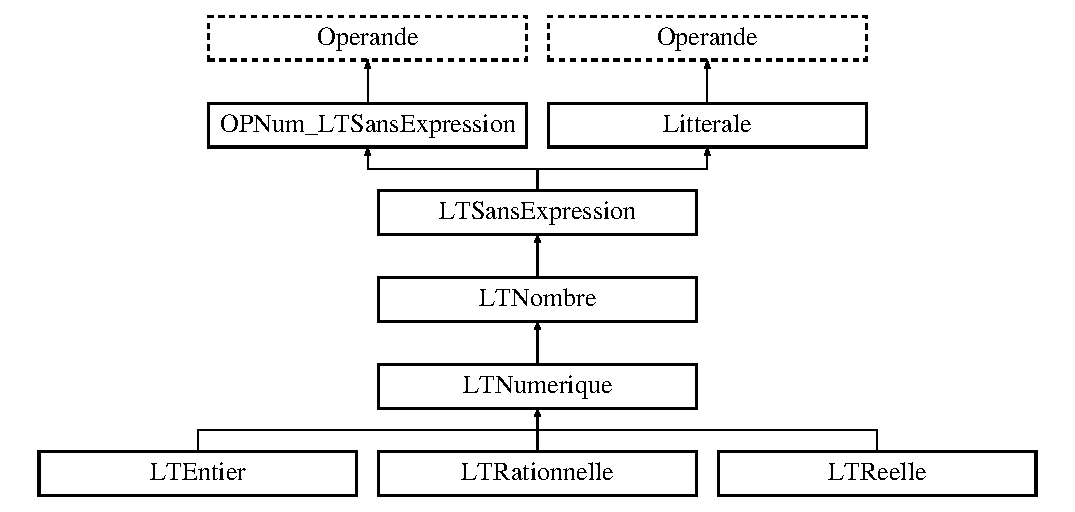
\includegraphics[height=6.000000cm]{class_l_t_numerique}
\end{center}
\end{figure}
\subsection*{Public Member Functions}
\begin{DoxyCompactItemize}
\item 
{\bfseries L\+T\+Numerique} (\hyperlink{class_l_t_atome}{L\+T\+Atome} $\ast$a=0)\hypertarget{class_l_t_numerique_afdba20ccf63d95ea51744804fbd712de}{}\label{class_l_t_numerique_afdba20ccf63d95ea51744804fbd712de}

\item 
{\bfseries L\+T\+Numerique} (\hyperlink{class_l_t_numerique}{L\+T\+Numerique} $\ast$n, \hyperlink{class_l_t_atome}{L\+T\+Atome} $\ast$a=0)\hypertarget{class_l_t_numerique_ada69a222a6bbcd5b2ef1b12106614448}{}\label{class_l_t_numerique_ada69a222a6bbcd5b2ef1b12106614448}

\item 
virtual \hyperlink{class_l_t_atome}{L\+T\+Atome} $\ast$ {\bfseries get\+Atome} () const \hypertarget{class_l_t_numerique_a92f56bd49c69390afba8321f189d282f}{}\label{class_l_t_numerique_a92f56bd49c69390afba8321f189d282f}

\item 
virtual void \hyperlink{class_l_t_numerique_a374425c7d4f14f7a4ac999a7048f7206}{afficher} () const  =0\hypertarget{class_l_t_numerique_a374425c7d4f14f7a4ac999a7048f7206}{}\label{class_l_t_numerique_a374425c7d4f14f7a4ac999a7048f7206}

\begin{DoxyCompactList}\small\item\em Fonction virtuelle affichant la litterale sur la sortie standart. \end{DoxyCompactList}\item 
virtual Q\+String \hyperlink{class_l_t_numerique_abef28b1b62ee356717f70f4317a44590}{get\+Text} () const  =0
\begin{DoxyCompactList}\small\item\em Fonction virtuelle renvoyant la litterale sous forme de texte. \end{DoxyCompactList}\item 
virtual \hyperlink{class_l_t_numerique}{L\+T\+Numerique} $\ast$ \hyperlink{class_l_t_numerique_a884056443dd30cd71c49b42b5ba63581}{clone} () const  =0
\begin{DoxyCompactList}\small\item\em Fonction virtuelle renvoyant une copie de l\textquotesingle{}instance. \end{DoxyCompactList}\item 
virtual \hyperlink{class_l_t_numerique}{L\+T\+Numerique} $\ast$ \hyperlink{class_l_t_numerique_a3963de62916188d01f93b1d0fdb42c7f}{simplifier} ()=0
\begin{DoxyCompactList}\small\item\em Fonction virtuelle simplifiant la litterale actuelle. \end{DoxyCompactList}\item 
virtual \hyperlink{class_l_t_numerique}{L\+T\+Numerique} $\ast$ {\bfseries operator-\/-\/} ()=0\hypertarget{class_l_t_numerique_ac3b8e78546185c08c3ed82e1ca16689d}{}\label{class_l_t_numerique_ac3b8e78546185c08c3ed82e1ca16689d}

\item 
virtual \hyperlink{class_l_t_numerique}{L\+T\+Numerique} $\ast$ \hyperlink{class_l_t_numerique_a9fb09223dc517fae452f4af0d50f6966}{operator+} (\hyperlink{class_l_t_numerique}{L\+T\+Numerique} $\ast$p)=0
\begin{DoxyCompactList}\small\item\em Addition entre un \hyperlink{class_l_t_complexe}{L\+T\+Complexe} et un \hyperlink{class_l_t_numerique}{L\+T\+Numerique}. \end{DoxyCompactList}\item 
virtual \hyperlink{class_l_t_complexe}{L\+T\+Complexe} $\ast$ \hyperlink{class_l_t_numerique_a615173a7cd77e649235d1c06d72726e7}{operator+} (\hyperlink{class_l_t_complexe}{L\+T\+Complexe} $\ast$p)=0
\begin{DoxyCompactList}\small\item\em Addition entre un \hyperlink{class_l_t_complexe}{L\+T\+Complexe} et un \hyperlink{class_l_t_complexe}{L\+T\+Complexe}. \end{DoxyCompactList}\item 
virtual \hyperlink{class_l_t_numerique}{L\+T\+Numerique} $\ast$ \hyperlink{class_l_t_numerique_a94d98eef8d391bdb925dbb70a1b35834}{operator-\/} (\hyperlink{class_l_t_numerique}{L\+T\+Numerique} $\ast$p)=0
\begin{DoxyCompactList}\small\item\em Soustraction entre un \hyperlink{class_l_t_complexe}{L\+T\+Complexe} et un \hyperlink{class_l_t_numerique}{L\+T\+Numerique}. \end{DoxyCompactList}\item 
virtual \hyperlink{class_l_t_complexe}{L\+T\+Complexe} $\ast$ \hyperlink{class_l_t_numerique_a45bbf62a5725c3b9c8a8a14d9be6ef47}{operator-\/} (\hyperlink{class_l_t_complexe}{L\+T\+Complexe} $\ast$p)=0
\begin{DoxyCompactList}\small\item\em Soustraction entre un \hyperlink{class_l_t_complexe}{L\+T\+Complexe} et un \hyperlink{class_l_t_complexe}{L\+T\+Complexe}. \end{DoxyCompactList}\item 
virtual \hyperlink{class_l_t_numerique}{L\+T\+Numerique} $\ast$ \hyperlink{class_l_t_numerique_aef374b7679c6b9b7901e0a4bbfce4cc3}{operator$\ast$} (\hyperlink{class_l_t_numerique}{L\+T\+Numerique} $\ast$p)=0
\begin{DoxyCompactList}\small\item\em Multiplication entre un \hyperlink{class_l_t_complexe}{L\+T\+Complexe} et un \hyperlink{class_l_t_numerique}{L\+T\+Numerique}. \end{DoxyCompactList}\item 
virtual \hyperlink{class_l_t_complexe}{L\+T\+Complexe} $\ast$ \hyperlink{class_l_t_numerique_a6991c6c854915c7bfd98634c791ab815}{operator$\ast$} (\hyperlink{class_l_t_complexe}{L\+T\+Complexe} $\ast$p)=0
\begin{DoxyCompactList}\small\item\em Multiplication entre un \hyperlink{class_l_t_complexe}{L\+T\+Complexe} et un \hyperlink{class_l_t_complexe}{L\+T\+Complexe}. \end{DoxyCompactList}\item 
virtual \hyperlink{class_l_t_numerique}{L\+T\+Numerique} $\ast$ \hyperlink{class_l_t_numerique_ab3acc500e7c92b2d1e05ebc65561b84a}{operator/} (\hyperlink{class_l_t_numerique}{L\+T\+Numerique} $\ast$p)=0
\begin{DoxyCompactList}\small\item\em Division entre un \hyperlink{class_l_t_complexe}{L\+T\+Complexe} et un \hyperlink{class_l_t_numerique}{L\+T\+Numerique}. \end{DoxyCompactList}\item 
virtual \hyperlink{class_l_t_complexe}{L\+T\+Complexe} $\ast$ \hyperlink{class_l_t_numerique_a223402e5b15e25f716bdd1981f59f39d}{operator/} (\hyperlink{class_l_t_complexe}{L\+T\+Complexe} $\ast$p)=0
\begin{DoxyCompactList}\small\item\em Division entre un \hyperlink{class_l_t_complexe}{L\+T\+Complexe} et un \hyperlink{class_l_t_numerique}{L\+T\+Numerique}. \end{DoxyCompactList}\end{DoxyCompactItemize}
\subsection*{Protected Attributes}
\begin{DoxyCompactItemize}
\item 
\hyperlink{class_l_t_atome}{L\+T\+Atome} $\ast$ {\bfseries identificateur}\hypertarget{class_l_t_numerique_abf20a2e6d19ae6a01b1114fd15460174}{}\label{class_l_t_numerique_abf20a2e6d19ae6a01b1114fd15460174}

\end{DoxyCompactItemize}
\subsection*{Friends}
\begin{DoxyCompactItemize}
\item 
bool {\bfseries operator==} (\hyperlink{class_l_t_numerique}{L\+T\+Numerique} \&l1, \hyperlink{class_l_t_numerique}{L\+T\+Numerique} \&l2)\hypertarget{class_l_t_numerique_ae22deea9ec68fc9e4b3844ce3e2a17b1}{}\label{class_l_t_numerique_ae22deea9ec68fc9e4b3844ce3e2a17b1}

\item 
bool {\bfseries operator!=} (\hyperlink{class_l_t_numerique}{L\+T\+Numerique} \&l1, \hyperlink{class_l_t_numerique}{L\+T\+Numerique} \&l2)\hypertarget{class_l_t_numerique_ac270ee2118c09d7357f163556710fe2a}{}\label{class_l_t_numerique_ac270ee2118c09d7357f163556710fe2a}

\item 
bool {\bfseries operator$<$} (\hyperlink{class_l_t_numerique}{L\+T\+Numerique} \&l1, \hyperlink{class_l_t_numerique}{L\+T\+Numerique} \&l2)\hypertarget{class_l_t_numerique_aff65692b26bbb7ecb049394d05de5e73}{}\label{class_l_t_numerique_aff65692b26bbb7ecb049394d05de5e73}

\item 
bool {\bfseries operator$<$=} (\hyperlink{class_l_t_numerique}{L\+T\+Numerique} \&l1, \hyperlink{class_l_t_numerique}{L\+T\+Numerique} \&l2)\hypertarget{class_l_t_numerique_aec3955c88443d36f9e378c47a1990058}{}\label{class_l_t_numerique_aec3955c88443d36f9e378c47a1990058}

\item 
bool {\bfseries operator$>$} (\hyperlink{class_l_t_numerique}{L\+T\+Numerique} \&l1, \hyperlink{class_l_t_numerique}{L\+T\+Numerique} \&l2)\hypertarget{class_l_t_numerique_a500bab8b4205a5a0b43a1760734b4b21}{}\label{class_l_t_numerique_a500bab8b4205a5a0b43a1760734b4b21}

\item 
bool {\bfseries operator$>$=} (\hyperlink{class_l_t_numerique}{L\+T\+Numerique} \&l1, \hyperlink{class_l_t_numerique}{L\+T\+Numerique} \&l2)\hypertarget{class_l_t_numerique_a5ed128e9026bda1a4529d31368e0aa1b}{}\label{class_l_t_numerique_a5ed128e9026bda1a4529d31368e0aa1b}

\end{DoxyCompactItemize}


\subsection{Member Function Documentation}
\index{L\+T\+Numerique@{L\+T\+Numerique}!clone@{clone}}
\index{clone@{clone}!L\+T\+Numerique@{L\+T\+Numerique}}
\subsubsection[{\texorpdfstring{clone() const  =0}{clone() const  =0}}]{\setlength{\rightskip}{0pt plus 5cm}virtual {\bf L\+T\+Numerique}$\ast$ L\+T\+Numerique\+::clone (
\begin{DoxyParamCaption}
{}
\end{DoxyParamCaption}
) const\hspace{0.3cm}{\ttfamily [pure virtual]}}\hypertarget{class_l_t_numerique_a884056443dd30cd71c49b42b5ba63581}{}\label{class_l_t_numerique_a884056443dd30cd71c49b42b5ba63581}


Fonction virtuelle renvoyant une copie de l\textquotesingle{}instance. 

\begin{DoxyReturn}{Returns}
Nouvelle litterale copiée 
\end{DoxyReturn}


Implements \hyperlink{class_l_t_nombre_a09ad6faddbb007746e41af6873bd1824}{L\+T\+Nombre}.



Implemented in \hyperlink{class_l_t_reelle_a1dac7c02dfa84815730d5f0396ef1519}{L\+T\+Reelle}, \hyperlink{class_l_t_rationnelle_a48b36c50460ce15674d1d72afb41daf3}{L\+T\+Rationnelle}, and \hyperlink{class_l_t_entier_afc21b025efd3feea0162053902b8d640}{L\+T\+Entier}.

\index{L\+T\+Numerique@{L\+T\+Numerique}!get\+Text@{get\+Text}}
\index{get\+Text@{get\+Text}!L\+T\+Numerique@{L\+T\+Numerique}}
\subsubsection[{\texorpdfstring{get\+Text() const  =0}{getText() const  =0}}]{\setlength{\rightskip}{0pt plus 5cm}virtual Q\+String L\+T\+Numerique\+::get\+Text (
\begin{DoxyParamCaption}
{}
\end{DoxyParamCaption}
) const\hspace{0.3cm}{\ttfamily [pure virtual]}}\hypertarget{class_l_t_numerique_abef28b1b62ee356717f70f4317a44590}{}\label{class_l_t_numerique_abef28b1b62ee356717f70f4317a44590}


Fonction virtuelle renvoyant la litterale sous forme de texte. 

\begin{DoxyReturn}{Returns}
\hyperlink{class_litterale}{Litterale} sous forme de texte 
\end{DoxyReturn}


Implements \hyperlink{class_l_t_nombre_a39fe941ec69bf013bc3be8b3e575c3d0}{L\+T\+Nombre}.



Implemented in \hyperlink{class_l_t_reelle_aa85d99c6c692e3fd51019630cfd88cc4}{L\+T\+Reelle}, \hyperlink{class_l_t_rationnelle_a7195f7e7ddfe6c5493932fe08785ac76}{L\+T\+Rationnelle}, and \hyperlink{class_l_t_entier_a735c05de25b1264a5b2bc603f63eed58}{L\+T\+Entier}.

\index{L\+T\+Numerique@{L\+T\+Numerique}!operator$\ast$@{operator$\ast$}}
\index{operator$\ast$@{operator$\ast$}!L\+T\+Numerique@{L\+T\+Numerique}}
\subsubsection[{\texorpdfstring{operator$\ast$(\+L\+T\+Numerique $\ast$p)=0}{operator*(LTNumerique *p)=0}}]{\setlength{\rightskip}{0pt plus 5cm}virtual {\bf L\+T\+Numerique}$\ast$ L\+T\+Numerique\+::operator$\ast$ (
\begin{DoxyParamCaption}
\item[{{\bf L\+T\+Numerique} $\ast$}]{p}
\end{DoxyParamCaption}
)\hspace{0.3cm}{\ttfamily [pure virtual]}}\hypertarget{class_l_t_numerique_aef374b7679c6b9b7901e0a4bbfce4cc3}{}\label{class_l_t_numerique_aef374b7679c6b9b7901e0a4bbfce4cc3}


Multiplication entre un \hyperlink{class_l_t_complexe}{L\+T\+Complexe} et un \hyperlink{class_l_t_numerique}{L\+T\+Numerique}. 


\begin{DoxyParams}{Parameters}
{\em p} & Variable à ajouter \\
\hline
\end{DoxyParams}
\begin{DoxyReturn}{Returns}
\hyperlink{class_l_t_nombre}{L\+T\+Nombre} créé 
\end{DoxyReturn}


Implements \hyperlink{class_l_t_nombre_af77bf71cb71f2409ee78ae8421958bfe}{L\+T\+Nombre}.



Implemented in \hyperlink{class_l_t_reelle_a29fb03f19d56023485233168814c5f55}{L\+T\+Reelle}, \hyperlink{class_l_t_rationnelle_a030b31d5a3dd1b24fc107d6da616731f}{L\+T\+Rationnelle}, and \hyperlink{class_l_t_entier_a77d0c8047664798243c81017c6402612}{L\+T\+Entier}.

\index{L\+T\+Numerique@{L\+T\+Numerique}!operator$\ast$@{operator$\ast$}}
\index{operator$\ast$@{operator$\ast$}!L\+T\+Numerique@{L\+T\+Numerique}}
\subsubsection[{\texorpdfstring{operator$\ast$(\+L\+T\+Complexe $\ast$p)=0}{operator*(LTComplexe *p)=0}}]{\setlength{\rightskip}{0pt plus 5cm}virtual {\bf L\+T\+Complexe}$\ast$ L\+T\+Numerique\+::operator$\ast$ (
\begin{DoxyParamCaption}
\item[{{\bf L\+T\+Complexe} $\ast$}]{p}
\end{DoxyParamCaption}
)\hspace{0.3cm}{\ttfamily [pure virtual]}}\hypertarget{class_l_t_numerique_a6991c6c854915c7bfd98634c791ab815}{}\label{class_l_t_numerique_a6991c6c854915c7bfd98634c791ab815}


Multiplication entre un \hyperlink{class_l_t_complexe}{L\+T\+Complexe} et un \hyperlink{class_l_t_complexe}{L\+T\+Complexe}. 


\begin{DoxyParams}{Parameters}
{\em p} & Variable à ajouter \\
\hline
\end{DoxyParams}
\begin{DoxyReturn}{Returns}
\hyperlink{class_l_t_complexe}{L\+T\+Complexe} créé 
\end{DoxyReturn}


Implements \hyperlink{class_l_t_nombre_a90743859f0a4197a698d44be68d5c47b}{L\+T\+Nombre}.



Implemented in \hyperlink{class_l_t_reelle_a6411ae704917972524001f81862814ff}{L\+T\+Reelle}, \hyperlink{class_l_t_rationnelle_a5243f9ce9fd277473bd95f873b32c1e5}{L\+T\+Rationnelle}, and \hyperlink{class_l_t_entier_a621d0a41b4347cd02f0c99052b9f8e55}{L\+T\+Entier}.

\index{L\+T\+Numerique@{L\+T\+Numerique}!operator+@{operator+}}
\index{operator+@{operator+}!L\+T\+Numerique@{L\+T\+Numerique}}
\subsubsection[{\texorpdfstring{operator+(\+L\+T\+Numerique $\ast$p)=0}{operator+(LTNumerique *p)=0}}]{\setlength{\rightskip}{0pt plus 5cm}virtual {\bf L\+T\+Numerique}$\ast$ L\+T\+Numerique\+::operator+ (
\begin{DoxyParamCaption}
\item[{{\bf L\+T\+Numerique} $\ast$}]{p}
\end{DoxyParamCaption}
)\hspace{0.3cm}{\ttfamily [pure virtual]}}\hypertarget{class_l_t_numerique_a9fb09223dc517fae452f4af0d50f6966}{}\label{class_l_t_numerique_a9fb09223dc517fae452f4af0d50f6966}


Addition entre un \hyperlink{class_l_t_complexe}{L\+T\+Complexe} et un \hyperlink{class_l_t_numerique}{L\+T\+Numerique}. 


\begin{DoxyParams}{Parameters}
{\em p} & Variable à ajouter \\
\hline
\end{DoxyParams}
\begin{DoxyReturn}{Returns}
\hyperlink{class_l_t_nombre}{L\+T\+Nombre} créé 
\end{DoxyReturn}


Implements \hyperlink{class_l_t_nombre_a3962ef35dcfd735800ed5630e55a1d81}{L\+T\+Nombre}.



Implemented in \hyperlink{class_l_t_reelle_a89bf36d07622d65ef879f8fbf14ffb88}{L\+T\+Reelle}, \hyperlink{class_l_t_rationnelle_ad9d63f8ad77ec94ecf8510af2cbea1d2}{L\+T\+Rationnelle}, and \hyperlink{class_l_t_entier_ab61b9d54516e57b37923433cbb76ced7}{L\+T\+Entier}.

\index{L\+T\+Numerique@{L\+T\+Numerique}!operator+@{operator+}}
\index{operator+@{operator+}!L\+T\+Numerique@{L\+T\+Numerique}}
\subsubsection[{\texorpdfstring{operator+(\+L\+T\+Complexe $\ast$p)=0}{operator+(LTComplexe *p)=0}}]{\setlength{\rightskip}{0pt plus 5cm}virtual {\bf L\+T\+Complexe}$\ast$ L\+T\+Numerique\+::operator+ (
\begin{DoxyParamCaption}
\item[{{\bf L\+T\+Complexe} $\ast$}]{p}
\end{DoxyParamCaption}
)\hspace{0.3cm}{\ttfamily [pure virtual]}}\hypertarget{class_l_t_numerique_a615173a7cd77e649235d1c06d72726e7}{}\label{class_l_t_numerique_a615173a7cd77e649235d1c06d72726e7}


Addition entre un \hyperlink{class_l_t_complexe}{L\+T\+Complexe} et un \hyperlink{class_l_t_complexe}{L\+T\+Complexe}. 


\begin{DoxyParams}{Parameters}
{\em p} & Variable à ajouter \\
\hline
\end{DoxyParams}
\begin{DoxyReturn}{Returns}
\hyperlink{class_l_t_complexe}{L\+T\+Complexe} créé 
\end{DoxyReturn}


Implements \hyperlink{class_l_t_nombre_a8caa60dd6bf935dc68e8a37bd527b4d8}{L\+T\+Nombre}.



Implemented in \hyperlink{class_l_t_reelle_af860cce772e4228c2a41654a074278c9}{L\+T\+Reelle}, \hyperlink{class_l_t_rationnelle_a2feef6c4dd95b53a2c8635f74fa30c8e}{L\+T\+Rationnelle}, and \hyperlink{class_l_t_entier_af87e5527f3e09fa388313b880ba92c84}{L\+T\+Entier}.

\index{L\+T\+Numerique@{L\+T\+Numerique}!operator-\/@{operator-\/}}
\index{operator-\/@{operator-\/}!L\+T\+Numerique@{L\+T\+Numerique}}
\subsubsection[{\texorpdfstring{operator-\/(\+L\+T\+Numerique $\ast$p)=0}{operator-(LTNumerique *p)=0}}]{\setlength{\rightskip}{0pt plus 5cm}virtual {\bf L\+T\+Numerique}$\ast$ L\+T\+Numerique\+::operator-\/ (
\begin{DoxyParamCaption}
\item[{{\bf L\+T\+Numerique} $\ast$}]{p}
\end{DoxyParamCaption}
)\hspace{0.3cm}{\ttfamily [pure virtual]}}\hypertarget{class_l_t_numerique_a94d98eef8d391bdb925dbb70a1b35834}{}\label{class_l_t_numerique_a94d98eef8d391bdb925dbb70a1b35834}


Soustraction entre un \hyperlink{class_l_t_complexe}{L\+T\+Complexe} et un \hyperlink{class_l_t_numerique}{L\+T\+Numerique}. 


\begin{DoxyParams}{Parameters}
{\em p} & Variable à ajouter \\
\hline
\end{DoxyParams}
\begin{DoxyReturn}{Returns}
\hyperlink{class_l_t_nombre}{L\+T\+Nombre} créé 
\end{DoxyReturn}


Implements \hyperlink{class_l_t_nombre_ade4345e2555976c45c433fcc6d91e417}{L\+T\+Nombre}.



Implemented in \hyperlink{class_l_t_reelle_ab531e728f5055d41887f590db44ac4d2}{L\+T\+Reelle}, \hyperlink{class_l_t_rationnelle_a397f4f28299295ff68b790420a6a0060}{L\+T\+Rationnelle}, and \hyperlink{class_l_t_entier_ae7d462d020affefeb6a348ae17ce8c95}{L\+T\+Entier}.

\index{L\+T\+Numerique@{L\+T\+Numerique}!operator-\/@{operator-\/}}
\index{operator-\/@{operator-\/}!L\+T\+Numerique@{L\+T\+Numerique}}
\subsubsection[{\texorpdfstring{operator-\/(\+L\+T\+Complexe $\ast$p)=0}{operator-(LTComplexe *p)=0}}]{\setlength{\rightskip}{0pt plus 5cm}virtual {\bf L\+T\+Complexe}$\ast$ L\+T\+Numerique\+::operator-\/ (
\begin{DoxyParamCaption}
\item[{{\bf L\+T\+Complexe} $\ast$}]{p}
\end{DoxyParamCaption}
)\hspace{0.3cm}{\ttfamily [pure virtual]}}\hypertarget{class_l_t_numerique_a45bbf62a5725c3b9c8a8a14d9be6ef47}{}\label{class_l_t_numerique_a45bbf62a5725c3b9c8a8a14d9be6ef47}


Soustraction entre un \hyperlink{class_l_t_complexe}{L\+T\+Complexe} et un \hyperlink{class_l_t_complexe}{L\+T\+Complexe}. 


\begin{DoxyParams}{Parameters}
{\em p} & Variable à ajouter \\
\hline
\end{DoxyParams}
\begin{DoxyReturn}{Returns}
\hyperlink{class_l_t_complexe}{L\+T\+Complexe} créé 
\end{DoxyReturn}


Implements \hyperlink{class_l_t_nombre_a60d335475d7b623f6f8ff513494e6572}{L\+T\+Nombre}.



Implemented in \hyperlink{class_l_t_reelle_a8f23a1ce94f266ab5b406769a94e88fe}{L\+T\+Reelle}, \hyperlink{class_l_t_rationnelle_a8412426bfe4d5c7b2d5377cfa4f0f154}{L\+T\+Rationnelle}, and \hyperlink{class_l_t_entier_a2fa9e6e1f2cdcdfb3fc5cd85985928e6}{L\+T\+Entier}.

\index{L\+T\+Numerique@{L\+T\+Numerique}!operator/@{operator/}}
\index{operator/@{operator/}!L\+T\+Numerique@{L\+T\+Numerique}}
\subsubsection[{\texorpdfstring{operator/(\+L\+T\+Numerique $\ast$p)=0}{operator/(LTNumerique *p)=0}}]{\setlength{\rightskip}{0pt plus 5cm}virtual {\bf L\+T\+Numerique}$\ast$ L\+T\+Numerique\+::operator/ (
\begin{DoxyParamCaption}
\item[{{\bf L\+T\+Numerique} $\ast$}]{p}
\end{DoxyParamCaption}
)\hspace{0.3cm}{\ttfamily [pure virtual]}}\hypertarget{class_l_t_numerique_ab3acc500e7c92b2d1e05ebc65561b84a}{}\label{class_l_t_numerique_ab3acc500e7c92b2d1e05ebc65561b84a}


Division entre un \hyperlink{class_l_t_complexe}{L\+T\+Complexe} et un \hyperlink{class_l_t_numerique}{L\+T\+Numerique}. 


\begin{DoxyParams}{Parameters}
{\em p} & Variable à ajouter \\
\hline
\end{DoxyParams}
\begin{DoxyReturn}{Returns}
\hyperlink{class_l_t_nombre}{L\+T\+Nombre} créé 
\end{DoxyReturn}


Implements \hyperlink{class_l_t_nombre_abfb3b0f925a6706222173779cf3f762d}{L\+T\+Nombre}.



Implemented in \hyperlink{class_l_t_reelle_a088c4683ed4077bceffca599f24fcee8}{L\+T\+Reelle}, \hyperlink{class_l_t_rationnelle_a9f82305c64896be366084ee6941933b1}{L\+T\+Rationnelle}, and \hyperlink{class_l_t_entier_abde7f75a9aec4852f4f624cf94080fdc}{L\+T\+Entier}.

\index{L\+T\+Numerique@{L\+T\+Numerique}!operator/@{operator/}}
\index{operator/@{operator/}!L\+T\+Numerique@{L\+T\+Numerique}}
\subsubsection[{\texorpdfstring{operator/(\+L\+T\+Complexe $\ast$p)=0}{operator/(LTComplexe *p)=0}}]{\setlength{\rightskip}{0pt plus 5cm}virtual {\bf L\+T\+Complexe}$\ast$ L\+T\+Numerique\+::operator/ (
\begin{DoxyParamCaption}
\item[{{\bf L\+T\+Complexe} $\ast$}]{p}
\end{DoxyParamCaption}
)\hspace{0.3cm}{\ttfamily [pure virtual]}}\hypertarget{class_l_t_numerique_a223402e5b15e25f716bdd1981f59f39d}{}\label{class_l_t_numerique_a223402e5b15e25f716bdd1981f59f39d}


Division entre un \hyperlink{class_l_t_complexe}{L\+T\+Complexe} et un \hyperlink{class_l_t_numerique}{L\+T\+Numerique}. 


\begin{DoxyParams}{Parameters}
{\em p} & Variable à ajouter \\
\hline
\end{DoxyParams}
\begin{DoxyReturn}{Returns}
\hyperlink{class_l_t_complexe}{L\+T\+Complexe} créé 
\end{DoxyReturn}


Implements \hyperlink{class_l_t_nombre_ae7e0f2dba7aba0f3251e18c5cfc60b5a}{L\+T\+Nombre}.



Implemented in \hyperlink{class_l_t_reelle_a8260eb6ee9db3bea9798c49d1993060d}{L\+T\+Reelle}, \hyperlink{class_l_t_rationnelle_a6a44ee4834907f1e97008a0f7e3f33a1}{L\+T\+Rationnelle}, and \hyperlink{class_l_t_entier_a59f046d2849150eba46ffbc1edcf6b95}{L\+T\+Entier}.

\index{L\+T\+Numerique@{L\+T\+Numerique}!simplifier@{simplifier}}
\index{simplifier@{simplifier}!L\+T\+Numerique@{L\+T\+Numerique}}
\subsubsection[{\texorpdfstring{simplifier()=0}{simplifier()=0}}]{\setlength{\rightskip}{0pt plus 5cm}virtual {\bf L\+T\+Numerique}$\ast$ L\+T\+Numerique\+::simplifier (
\begin{DoxyParamCaption}
{}
\end{DoxyParamCaption}
)\hspace{0.3cm}{\ttfamily [pure virtual]}}\hypertarget{class_l_t_numerique_a3963de62916188d01f93b1d0fdb42c7f}{}\label{class_l_t_numerique_a3963de62916188d01f93b1d0fdb42c7f}


Fonction virtuelle simplifiant la litterale actuelle. 

\begin{DoxyReturn}{Returns}
Nouvelle litterale copiée 
\end{DoxyReturn}


Implements \hyperlink{class_l_t_nombre_a6aa1593c8c0956bb5412bfee3c15b085}{L\+T\+Nombre}.



Implemented in \hyperlink{class_l_t_reelle_aaaf23323d16d13b2ec7595c6aa07935f}{L\+T\+Reelle}, \hyperlink{class_l_t_rationnelle_afefcccb71e7fd20491e8f14aef88dd6e}{L\+T\+Rationnelle}, and \hyperlink{class_l_t_entier_a3dd0959762240ef5cbe0a62970728ddf}{L\+T\+Entier}.



The documentation for this class was generated from the following file\+:\begin{DoxyCompactItemize}
\item 
ltnumerique.\+h\end{DoxyCompactItemize}

\hypertarget{class_l_t_programme}{}\section{L\+T\+Programme Class Reference}
\label{class_l_t_programme}\index{L\+T\+Programme@{L\+T\+Programme}}
Inheritance diagram for L\+T\+Programme\+:\begin{figure}[H]
\begin{center}
\leavevmode
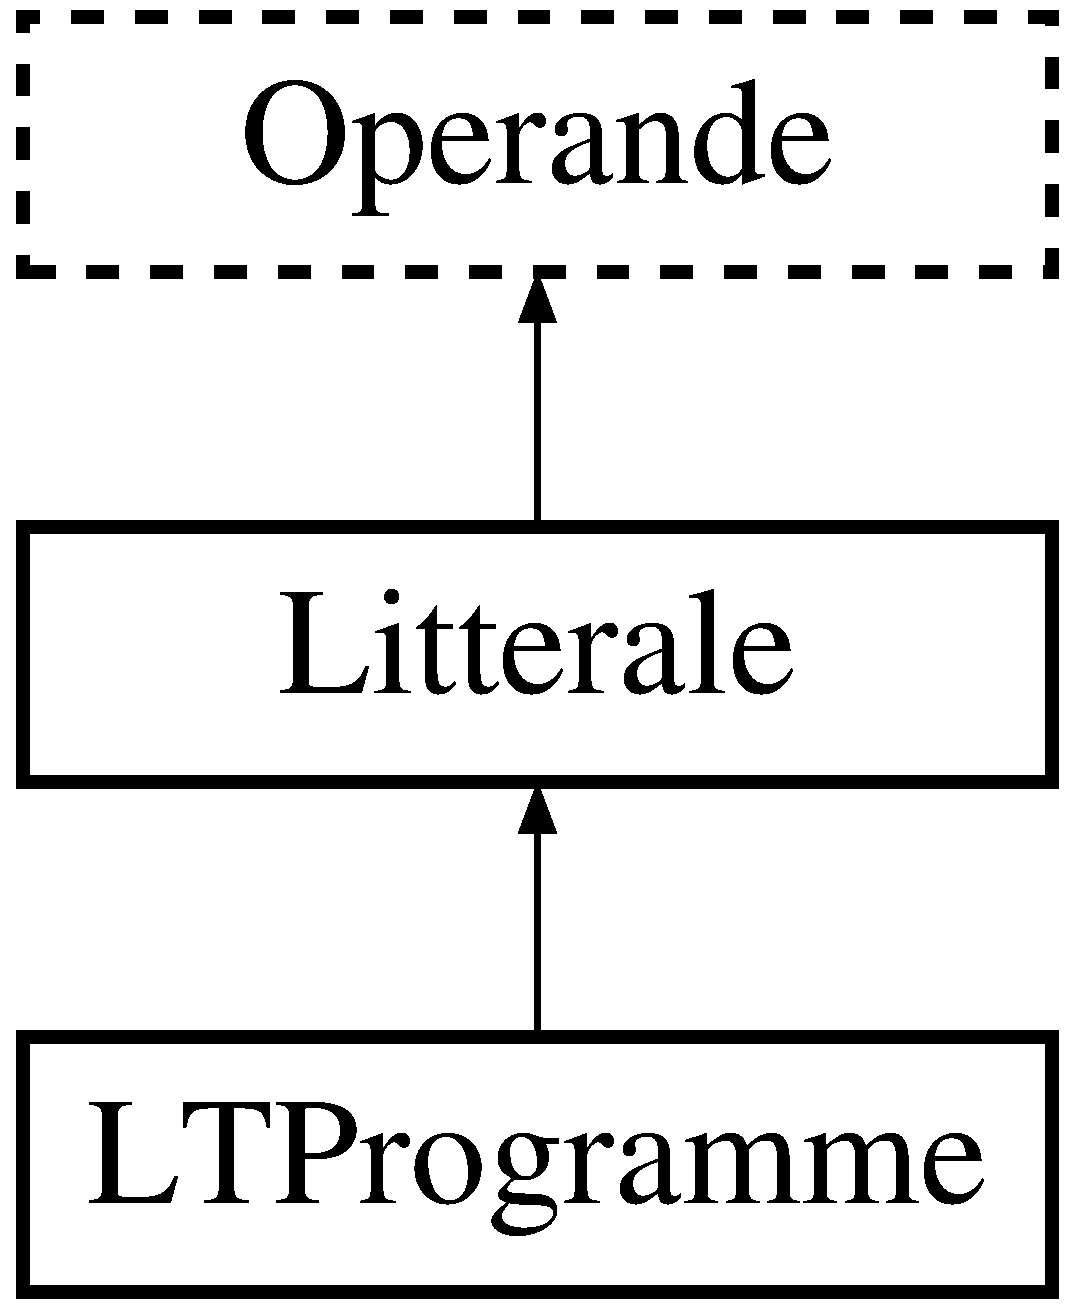
\includegraphics[height=3.000000cm]{class_l_t_programme}
\end{center}
\end{figure}
\subsection*{Public Member Functions}
\begin{DoxyCompactItemize}
\item 
{\bfseries L\+T\+Programme} (\hyperlink{class_l_t_atome}{L\+T\+Atome} id, Q\+List$<$ \hyperlink{class_operande}{Operande} $\ast$ $>$ list)\hypertarget{class_l_t_programme_a3a7dcba1419be15c4ca428c3b63423c9}{}\label{class_l_t_programme_a3a7dcba1419be15c4ca428c3b63423c9}

\item 
{\bfseries L\+T\+Programme} (Q\+List$<$ \hyperlink{class_operande}{Operande} $\ast$ $>$ list)\hypertarget{class_l_t_programme_a6bcc09bf64964e759b2ec3c0553ea97f}{}\label{class_l_t_programme_a6bcc09bf64964e759b2ec3c0553ea97f}

\item 
virtual void \hyperlink{class_l_t_programme_a245492a9909248573dfab29fe4f7b4ef}{afficher} () const \hypertarget{class_l_t_programme_a245492a9909248573dfab29fe4f7b4ef}{}\label{class_l_t_programme_a245492a9909248573dfab29fe4f7b4ef}

\begin{DoxyCompactList}\small\item\em Fonction virtuelle affichant la litterale sur la sortie standart. \end{DoxyCompactList}\item 
virtual Q\+String \hyperlink{class_l_t_programme_ad5f8e3d531b8a456944d806096881022}{get\+Text} () const 
\begin{DoxyCompactList}\small\item\em Fonction virtuelle renvoyant la litterale sous forme de texte. \end{DoxyCompactList}\item 
virtual Q\+List$<$ \hyperlink{class_operande}{Operande} $\ast$ $>$ {\bfseries get\+List\+Operande} ()\hypertarget{class_l_t_programme_aa2d0b7cd9ab8fde8107aecf4731ca1f4}{}\label{class_l_t_programme_aa2d0b7cd9ab8fde8107aecf4731ca1f4}

\item 
virtual \hyperlink{class_l_t_programme}{L\+T\+Programme} $\ast$ \hyperlink{class_l_t_programme_a1ae271a87f8b770aec069aa6dec3b84b}{clone} () const 
\begin{DoxyCompactList}\small\item\em Fonction virtuelle renvoyant une copie de l\textquotesingle{}instance. \end{DoxyCompactList}\item 
virtual \hyperlink{class_litterale}{Litterale} $\ast$ \hyperlink{class_l_t_programme_a7bfe6b6140e56fc578ed5dce2e2d9ea5}{simplifier} ()
\begin{DoxyCompactList}\small\item\em Fonction virtuelle simplifiant la litterale actuelle. \end{DoxyCompactList}\end{DoxyCompactItemize}


\subsection{Member Function Documentation}
\index{L\+T\+Programme@{L\+T\+Programme}!clone@{clone}}
\index{clone@{clone}!L\+T\+Programme@{L\+T\+Programme}}
\subsubsection[{\texorpdfstring{clone() const }{clone() const }}]{\setlength{\rightskip}{0pt plus 5cm}virtual {\bf L\+T\+Programme}$\ast$ L\+T\+Programme\+::clone (
\begin{DoxyParamCaption}
{}
\end{DoxyParamCaption}
) const\hspace{0.3cm}{\ttfamily [inline]}, {\ttfamily [virtual]}}\hypertarget{class_l_t_programme_a1ae271a87f8b770aec069aa6dec3b84b}{}\label{class_l_t_programme_a1ae271a87f8b770aec069aa6dec3b84b}


Fonction virtuelle renvoyant une copie de l\textquotesingle{}instance. 

\begin{DoxyReturn}{Returns}
Nouvelle litterale copiée 
\end{DoxyReturn}


Implements \hyperlink{class_litterale_a08967178d22c3d69e6c3e86ea8c85888}{Litterale}.

\index{L\+T\+Programme@{L\+T\+Programme}!get\+Text@{get\+Text}}
\index{get\+Text@{get\+Text}!L\+T\+Programme@{L\+T\+Programme}}
\subsubsection[{\texorpdfstring{get\+Text() const }{getText() const }}]{\setlength{\rightskip}{0pt plus 5cm}virtual Q\+String L\+T\+Programme\+::get\+Text (
\begin{DoxyParamCaption}
{}
\end{DoxyParamCaption}
) const\hspace{0.3cm}{\ttfamily [inline]}, {\ttfamily [virtual]}}\hypertarget{class_l_t_programme_ad5f8e3d531b8a456944d806096881022}{}\label{class_l_t_programme_ad5f8e3d531b8a456944d806096881022}


Fonction virtuelle renvoyant la litterale sous forme de texte. 

\begin{DoxyReturn}{Returns}
\hyperlink{class_litterale}{Litterale} sous forme de texte 
\end{DoxyReturn}


Implements \hyperlink{class_litterale_a780075c00abf31efb87e7c28843ea029}{Litterale}.

\index{L\+T\+Programme@{L\+T\+Programme}!simplifier@{simplifier}}
\index{simplifier@{simplifier}!L\+T\+Programme@{L\+T\+Programme}}
\subsubsection[{\texorpdfstring{simplifier()}{simplifier()}}]{\setlength{\rightskip}{0pt plus 5cm}virtual {\bf Litterale}$\ast$ L\+T\+Programme\+::simplifier (
\begin{DoxyParamCaption}
{}
\end{DoxyParamCaption}
)\hspace{0.3cm}{\ttfamily [inline]}, {\ttfamily [virtual]}}\hypertarget{class_l_t_programme_a7bfe6b6140e56fc578ed5dce2e2d9ea5}{}\label{class_l_t_programme_a7bfe6b6140e56fc578ed5dce2e2d9ea5}


Fonction virtuelle simplifiant la litterale actuelle. 

\begin{DoxyReturn}{Returns}
Nouvelle litterale copiée 
\end{DoxyReturn}


Implements \hyperlink{class_litterale_af33a0c1a4a9a5bb687da112b12f0e6e6}{Litterale}.



The documentation for this class was generated from the following file\+:\begin{DoxyCompactItemize}
\item 
ltprogramme.\+h\end{DoxyCompactItemize}

\hypertarget{class_l_t_rationnelle}{}\section{L\+T\+Rationnelle Class Reference}
\label{class_l_t_rationnelle}\index{L\+T\+Rationnelle@{L\+T\+Rationnelle}}
Inheritance diagram for L\+T\+Rationnelle\+:\begin{figure}[H]
\begin{center}
\leavevmode
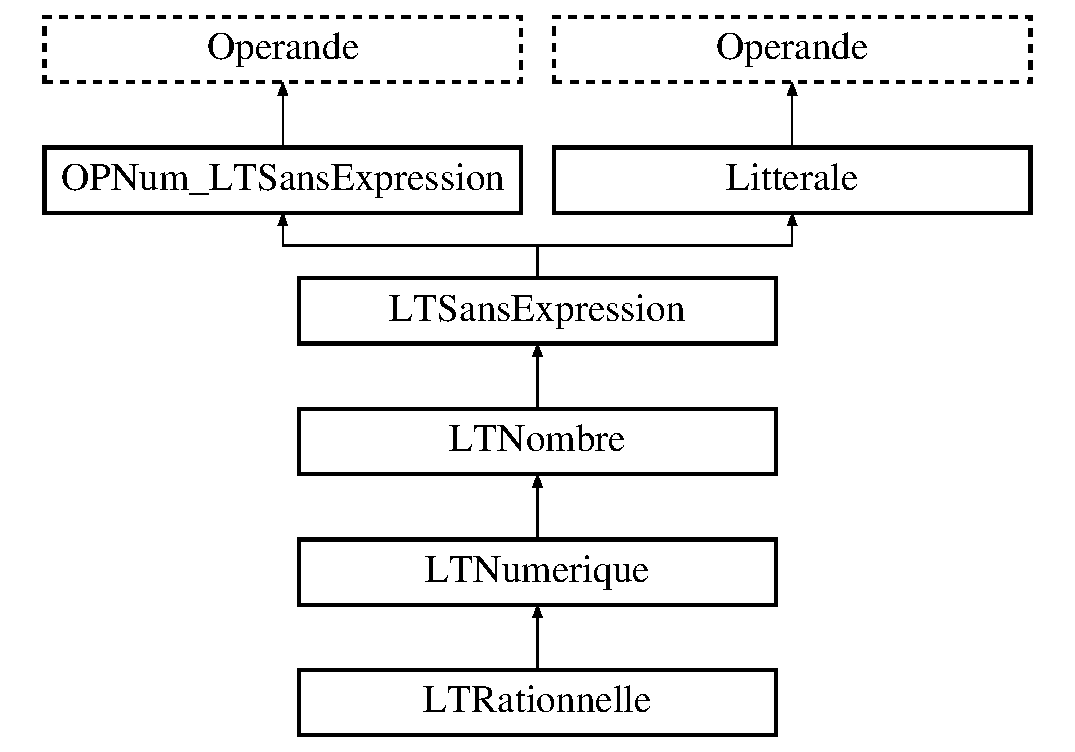
\includegraphics[height=6.000000cm]{class_l_t_rationnelle}
\end{center}
\end{figure}
\subsection*{Public Member Functions}
\begin{DoxyCompactItemize}
\item 
{\bfseries L\+T\+Rationnelle} (int v1, int v2, \hyperlink{class_l_t_atome}{L\+T\+Atome} $\ast$a=0)\hypertarget{class_l_t_rationnelle_ae6a4968b9cb89e964456c0a84ce2e4a8}{}\label{class_l_t_rationnelle_ae6a4968b9cb89e964456c0a84ce2e4a8}

\item 
{\bfseries L\+T\+Rationnelle} (Q\+String v1, Q\+String v2, \hyperlink{class_l_t_atome}{L\+T\+Atome} $\ast$a=0)\hypertarget{class_l_t_rationnelle_a518d0f2b06a9a8cf156bff2f693dd8b5}{}\label{class_l_t_rationnelle_a518d0f2b06a9a8cf156bff2f693dd8b5}

\item 
{\bfseries L\+T\+Rationnelle} (const \hyperlink{class_l_t_rationnelle}{L\+T\+Rationnelle} \&r, \hyperlink{class_l_t_atome}{L\+T\+Atome} $\ast$a=0)\hypertarget{class_l_t_rationnelle_ac82409ba58cce0624f0313dca86d979e}{}\label{class_l_t_rationnelle_ac82409ba58cce0624f0313dca86d979e}

\item 
{\bfseries L\+T\+Rationnelle} (const \hyperlink{class_l_t_entier}{L\+T\+Entier} \&r, \hyperlink{class_l_t_atome}{L\+T\+Atome} $\ast$a=0)\hypertarget{class_l_t_rationnelle_a12619dcec36d1bd347ec3c73a099d19c}{}\label{class_l_t_rationnelle_a12619dcec36d1bd347ec3c73a099d19c}

\item 
int {\bfseries pgcd} (unsigned int a, unsigned int b)\hypertarget{class_l_t_rationnelle_a8cc57db0cea018c34bfa9bc925913f93}{}\label{class_l_t_rationnelle_a8cc57db0cea018c34bfa9bc925913f93}

\item 
int {\bfseries get\+E1} () const \hypertarget{class_l_t_rationnelle_a425cc22d9f6605840866937382cffd2b}{}\label{class_l_t_rationnelle_a425cc22d9f6605840866937382cffd2b}

\item 
void {\bfseries set\+E1} (int v)\hypertarget{class_l_t_rationnelle_adedc58119f858549443fa0dc7ff1c34f}{}\label{class_l_t_rationnelle_adedc58119f858549443fa0dc7ff1c34f}

\item 
int {\bfseries get\+E2} () const \hypertarget{class_l_t_rationnelle_a3774fb07aa6fab1262b95f13b066ac8c}{}\label{class_l_t_rationnelle_a3774fb07aa6fab1262b95f13b066ac8c}

\item 
void {\bfseries set\+E2} (int v)\hypertarget{class_l_t_rationnelle_a07f9a5a2c84b036a34a90634fbb886e4}{}\label{class_l_t_rationnelle_a07f9a5a2c84b036a34a90634fbb886e4}

\item 
void {\bfseries set\+E1} (Q\+String v)\hypertarget{class_l_t_rationnelle_a44b8d833c4cacecef2ebb74ff98b408b}{}\label{class_l_t_rationnelle_a44b8d833c4cacecef2ebb74ff98b408b}

\item 
void {\bfseries set\+E2} (Q\+String v)\hypertarget{class_l_t_rationnelle_a0bcf0dccc893e5039ed5a702150b5e07}{}\label{class_l_t_rationnelle_a0bcf0dccc893e5039ed5a702150b5e07}

\item 
Q\+String {\bfseries get\+Separator} () const \hypertarget{class_l_t_rationnelle_a7a29c24022807ab7cba1513ac3ff085c}{}\label{class_l_t_rationnelle_a7a29c24022807ab7cba1513ac3ff085c}

\item 
virtual void \hyperlink{class_l_t_rationnelle_ab77a7d22c9b666207722cd389e4d37a0}{afficher} () const \hypertarget{class_l_t_rationnelle_ab77a7d22c9b666207722cd389e4d37a0}{}\label{class_l_t_rationnelle_ab77a7d22c9b666207722cd389e4d37a0}

\begin{DoxyCompactList}\small\item\em Fonction virtuelle affichant la litterale sur la sortie standart. \end{DoxyCompactList}\item 
virtual Q\+String \hyperlink{class_l_t_rationnelle_a7195f7e7ddfe6c5493932fe08785ac76}{get\+Text} () const 
\begin{DoxyCompactList}\small\item\em Fonction virtuelle renvoyant la litterale sous forme de texte. \end{DoxyCompactList}\item 
virtual \hyperlink{class_l_t_rationnelle}{L\+T\+Rationnelle} $\ast$ \hyperlink{class_l_t_rationnelle_a48b36c50460ce15674d1d72afb41daf3}{clone} () const 
\begin{DoxyCompactList}\small\item\em Fonction virtuelle renvoyant une copie de l\textquotesingle{}instance. \end{DoxyCompactList}\item 
virtual \hyperlink{class_l_t_numerique}{L\+T\+Numerique} $\ast$ \hyperlink{class_l_t_rationnelle_afefcccb71e7fd20491e8f14aef88dd6e}{simplifier} ()
\begin{DoxyCompactList}\small\item\em Fonction virtuelle simplifiant la litterale actuelle. \end{DoxyCompactList}\item 
virtual \hyperlink{class_l_t_rationnelle}{L\+T\+Rationnelle} $\ast$ {\bfseries operator-\/-\/} ()\hypertarget{class_l_t_rationnelle_a73e30e2242e48cc7c721b10e6654a5bb}{}\label{class_l_t_rationnelle_a73e30e2242e48cc7c721b10e6654a5bb}

\item 
virtual \hyperlink{class_l_t_numerique}{L\+T\+Numerique} $\ast$ \hyperlink{class_l_t_rationnelle_ad9d63f8ad77ec94ecf8510af2cbea1d2}{operator+} (\hyperlink{class_l_t_numerique}{L\+T\+Numerique} $\ast$p)
\begin{DoxyCompactList}\small\item\em Addition entre un \hyperlink{class_l_t_complexe}{L\+T\+Complexe} et un \hyperlink{class_l_t_numerique}{L\+T\+Numerique}. \end{DoxyCompactList}\item 
virtual \hyperlink{class_l_t_complexe}{L\+T\+Complexe} $\ast$ \hyperlink{class_l_t_rationnelle_a2feef6c4dd95b53a2c8635f74fa30c8e}{operator+} (\hyperlink{class_l_t_complexe}{L\+T\+Complexe} $\ast$p)
\begin{DoxyCompactList}\small\item\em Addition entre un \hyperlink{class_l_t_complexe}{L\+T\+Complexe} et un \hyperlink{class_l_t_complexe}{L\+T\+Complexe}. \end{DoxyCompactList}\item 
virtual \hyperlink{class_l_t_numerique}{L\+T\+Numerique} $\ast$ \hyperlink{class_l_t_rationnelle_a397f4f28299295ff68b790420a6a0060}{operator-\/} (\hyperlink{class_l_t_numerique}{L\+T\+Numerique} $\ast$p)
\begin{DoxyCompactList}\small\item\em Soustraction entre un \hyperlink{class_l_t_complexe}{L\+T\+Complexe} et un \hyperlink{class_l_t_numerique}{L\+T\+Numerique}. \end{DoxyCompactList}\item 
virtual \hyperlink{class_l_t_complexe}{L\+T\+Complexe} $\ast$ \hyperlink{class_l_t_rationnelle_a8412426bfe4d5c7b2d5377cfa4f0f154}{operator-\/} (\hyperlink{class_l_t_complexe}{L\+T\+Complexe} $\ast$p)
\begin{DoxyCompactList}\small\item\em Soustraction entre un \hyperlink{class_l_t_complexe}{L\+T\+Complexe} et un \hyperlink{class_l_t_complexe}{L\+T\+Complexe}. \end{DoxyCompactList}\item 
virtual \hyperlink{class_l_t_numerique}{L\+T\+Numerique} $\ast$ \hyperlink{class_l_t_rationnelle_a030b31d5a3dd1b24fc107d6da616731f}{operator$\ast$} (\hyperlink{class_l_t_numerique}{L\+T\+Numerique} $\ast$p)
\begin{DoxyCompactList}\small\item\em Multiplication entre un \hyperlink{class_l_t_complexe}{L\+T\+Complexe} et un \hyperlink{class_l_t_numerique}{L\+T\+Numerique}. \end{DoxyCompactList}\item 
virtual \hyperlink{class_l_t_complexe}{L\+T\+Complexe} $\ast$ \hyperlink{class_l_t_rationnelle_a5243f9ce9fd277473bd95f873b32c1e5}{operator$\ast$} (\hyperlink{class_l_t_complexe}{L\+T\+Complexe} $\ast$p)
\begin{DoxyCompactList}\small\item\em Multiplication entre un \hyperlink{class_l_t_complexe}{L\+T\+Complexe} et un \hyperlink{class_l_t_complexe}{L\+T\+Complexe}. \end{DoxyCompactList}\item 
virtual \hyperlink{class_l_t_numerique}{L\+T\+Numerique} $\ast$ \hyperlink{class_l_t_rationnelle_a9f82305c64896be366084ee6941933b1}{operator/} (\hyperlink{class_l_t_numerique}{L\+T\+Numerique} $\ast$p)
\begin{DoxyCompactList}\small\item\em Division entre un \hyperlink{class_l_t_complexe}{L\+T\+Complexe} et un \hyperlink{class_l_t_numerique}{L\+T\+Numerique}. \end{DoxyCompactList}\item 
virtual \hyperlink{class_l_t_complexe}{L\+T\+Complexe} $\ast$ \hyperlink{class_l_t_rationnelle_a6a44ee4834907f1e97008a0f7e3f33a1}{operator/} (\hyperlink{class_l_t_complexe}{L\+T\+Complexe} $\ast$p)
\begin{DoxyCompactList}\small\item\em Division entre un \hyperlink{class_l_t_complexe}{L\+T\+Complexe} et un \hyperlink{class_l_t_numerique}{L\+T\+Numerique}. \end{DoxyCompactList}\end{DoxyCompactItemize}
\subsection*{Static Public Attributes}
\begin{DoxyCompactItemize}
\item 
static const \hyperlink{class_l_t_rationnelle}{L\+T\+Rationnelle} {\bfseries zero} = \hyperlink{class_l_t_rationnelle}{L\+T\+Rationnelle}(0,1)\hypertarget{class_l_t_rationnelle_a9189dabc14c138f122c298a9f7919547}{}\label{class_l_t_rationnelle_a9189dabc14c138f122c298a9f7919547}

\end{DoxyCompactItemize}
\subsection*{Friends}
\begin{DoxyCompactItemize}
\item 
bool {\bfseries operator==} (\hyperlink{class_l_t_rationnelle}{L\+T\+Rationnelle} \&l1, \hyperlink{class_l_t_rationnelle}{L\+T\+Rationnelle} \&l2)\hypertarget{class_l_t_rationnelle_a4a1c3b9abfc9cf3bd7086fafb9e4ba0a}{}\label{class_l_t_rationnelle_a4a1c3b9abfc9cf3bd7086fafb9e4ba0a}

\item 
bool {\bfseries operator==} (\hyperlink{class_l_t_rationnelle}{L\+T\+Rationnelle} \&l1, \hyperlink{class_l_t_entier}{L\+T\+Entier} \&l2)\hypertarget{class_l_t_rationnelle_a876ef3ed5b945dd9d215467114da113e}{}\label{class_l_t_rationnelle_a876ef3ed5b945dd9d215467114da113e}

\item 
bool {\bfseries operator==} (\hyperlink{class_l_t_rationnelle}{L\+T\+Rationnelle} \&l1, \hyperlink{class_l_t_reelle}{L\+T\+Reelle} \&l2)\hypertarget{class_l_t_rationnelle_a777f8cc6504fb965bfb471d7d8ef88d1}{}\label{class_l_t_rationnelle_a777f8cc6504fb965bfb471d7d8ef88d1}

\item 
bool {\bfseries operator$<$} (\hyperlink{class_l_t_rationnelle}{L\+T\+Rationnelle} \&l1, \hyperlink{class_l_t_rationnelle}{L\+T\+Rationnelle} \&l2)\hypertarget{class_l_t_rationnelle_a733e4b41e081d731409ecc6d5bc7acd5}{}\label{class_l_t_rationnelle_a733e4b41e081d731409ecc6d5bc7acd5}

\item 
bool {\bfseries operator$<$} (\hyperlink{class_l_t_rationnelle}{L\+T\+Rationnelle} \&l1, \hyperlink{class_l_t_entier}{L\+T\+Entier} \&l2)\hypertarget{class_l_t_rationnelle_a1ca22dd7f4e80d45917fbaf48944b891}{}\label{class_l_t_rationnelle_a1ca22dd7f4e80d45917fbaf48944b891}

\item 
bool {\bfseries operator$<$} (\hyperlink{class_l_t_rationnelle}{L\+T\+Rationnelle} \&l1, \hyperlink{class_l_t_reelle}{L\+T\+Reelle} \&l2)\hypertarget{class_l_t_rationnelle_ad8107b1bd1525b558a2c51db0f4167cc}{}\label{class_l_t_rationnelle_ad8107b1bd1525b558a2c51db0f4167cc}

\end{DoxyCompactItemize}
\subsection*{Additional Inherited Members}


\subsection{Member Function Documentation}
\index{L\+T\+Rationnelle@{L\+T\+Rationnelle}!clone@{clone}}
\index{clone@{clone}!L\+T\+Rationnelle@{L\+T\+Rationnelle}}
\subsubsection[{\texorpdfstring{clone() const }{clone() const }}]{\setlength{\rightskip}{0pt plus 5cm}{\bf L\+T\+Rationnelle} $\ast$ L\+T\+Rationnelle\+::clone (
\begin{DoxyParamCaption}
{}
\end{DoxyParamCaption}
) const\hspace{0.3cm}{\ttfamily [virtual]}}\hypertarget{class_l_t_rationnelle_a48b36c50460ce15674d1d72afb41daf3}{}\label{class_l_t_rationnelle_a48b36c50460ce15674d1d72afb41daf3}


Fonction virtuelle renvoyant une copie de l\textquotesingle{}instance. 

\begin{DoxyReturn}{Returns}
Nouvelle litterale copiée 
\end{DoxyReturn}


Implements \hyperlink{class_l_t_numerique_a884056443dd30cd71c49b42b5ba63581}{L\+T\+Numerique}.

\index{L\+T\+Rationnelle@{L\+T\+Rationnelle}!get\+Text@{get\+Text}}
\index{get\+Text@{get\+Text}!L\+T\+Rationnelle@{L\+T\+Rationnelle}}
\subsubsection[{\texorpdfstring{get\+Text() const }{getText() const }}]{\setlength{\rightskip}{0pt plus 5cm}Q\+String L\+T\+Rationnelle\+::get\+Text (
\begin{DoxyParamCaption}
{}
\end{DoxyParamCaption}
) const\hspace{0.3cm}{\ttfamily [virtual]}}\hypertarget{class_l_t_rationnelle_a7195f7e7ddfe6c5493932fe08785ac76}{}\label{class_l_t_rationnelle_a7195f7e7ddfe6c5493932fe08785ac76}


Fonction virtuelle renvoyant la litterale sous forme de texte. 

\begin{DoxyReturn}{Returns}
\hyperlink{class_litterale}{Litterale} sous forme de texte 
\end{DoxyReturn}


Implements \hyperlink{class_l_t_numerique_abef28b1b62ee356717f70f4317a44590}{L\+T\+Numerique}.

\index{L\+T\+Rationnelle@{L\+T\+Rationnelle}!operator$\ast$@{operator$\ast$}}
\index{operator$\ast$@{operator$\ast$}!L\+T\+Rationnelle@{L\+T\+Rationnelle}}
\subsubsection[{\texorpdfstring{operator$\ast$(\+L\+T\+Numerique $\ast$p)}{operator*(LTNumerique *p)}}]{\setlength{\rightskip}{0pt plus 5cm}{\bf L\+T\+Numerique} $\ast$ L\+T\+Rationnelle\+::operator$\ast$ (
\begin{DoxyParamCaption}
\item[{{\bf L\+T\+Numerique} $\ast$}]{p}
\end{DoxyParamCaption}
)\hspace{0.3cm}{\ttfamily [virtual]}}\hypertarget{class_l_t_rationnelle_a030b31d5a3dd1b24fc107d6da616731f}{}\label{class_l_t_rationnelle_a030b31d5a3dd1b24fc107d6da616731f}


Multiplication entre un \hyperlink{class_l_t_complexe}{L\+T\+Complexe} et un \hyperlink{class_l_t_numerique}{L\+T\+Numerique}. 


\begin{DoxyParams}{Parameters}
{\em p} & Variable à ajouter \\
\hline
\end{DoxyParams}
\begin{DoxyReturn}{Returns}
\hyperlink{class_l_t_nombre}{L\+T\+Nombre} créé 
\end{DoxyReturn}


Implements \hyperlink{class_l_t_numerique_aef374b7679c6b9b7901e0a4bbfce4cc3}{L\+T\+Numerique}.

\index{L\+T\+Rationnelle@{L\+T\+Rationnelle}!operator$\ast$@{operator$\ast$}}
\index{operator$\ast$@{operator$\ast$}!L\+T\+Rationnelle@{L\+T\+Rationnelle}}
\subsubsection[{\texorpdfstring{operator$\ast$(\+L\+T\+Complexe $\ast$p)}{operator*(LTComplexe *p)}}]{\setlength{\rightskip}{0pt plus 5cm}{\bf L\+T\+Complexe} $\ast$ L\+T\+Rationnelle\+::operator$\ast$ (
\begin{DoxyParamCaption}
\item[{{\bf L\+T\+Complexe} $\ast$}]{p}
\end{DoxyParamCaption}
)\hspace{0.3cm}{\ttfamily [virtual]}}\hypertarget{class_l_t_rationnelle_a5243f9ce9fd277473bd95f873b32c1e5}{}\label{class_l_t_rationnelle_a5243f9ce9fd277473bd95f873b32c1e5}


Multiplication entre un \hyperlink{class_l_t_complexe}{L\+T\+Complexe} et un \hyperlink{class_l_t_complexe}{L\+T\+Complexe}. 


\begin{DoxyParams}{Parameters}
{\em p} & Variable à ajouter \\
\hline
\end{DoxyParams}
\begin{DoxyReturn}{Returns}
\hyperlink{class_l_t_complexe}{L\+T\+Complexe} créé 
\end{DoxyReturn}


Implements \hyperlink{class_l_t_numerique_a6991c6c854915c7bfd98634c791ab815}{L\+T\+Numerique}.

\index{L\+T\+Rationnelle@{L\+T\+Rationnelle}!operator+@{operator+}}
\index{operator+@{operator+}!L\+T\+Rationnelle@{L\+T\+Rationnelle}}
\subsubsection[{\texorpdfstring{operator+(\+L\+T\+Numerique $\ast$p)}{operator+(LTNumerique *p)}}]{\setlength{\rightskip}{0pt plus 5cm}{\bf L\+T\+Numerique} $\ast$ L\+T\+Rationnelle\+::operator+ (
\begin{DoxyParamCaption}
\item[{{\bf L\+T\+Numerique} $\ast$}]{p}
\end{DoxyParamCaption}
)\hspace{0.3cm}{\ttfamily [virtual]}}\hypertarget{class_l_t_rationnelle_ad9d63f8ad77ec94ecf8510af2cbea1d2}{}\label{class_l_t_rationnelle_ad9d63f8ad77ec94ecf8510af2cbea1d2}


Addition entre un \hyperlink{class_l_t_complexe}{L\+T\+Complexe} et un \hyperlink{class_l_t_numerique}{L\+T\+Numerique}. 


\begin{DoxyParams}{Parameters}
{\em p} & Variable à ajouter \\
\hline
\end{DoxyParams}
\begin{DoxyReturn}{Returns}
\hyperlink{class_l_t_nombre}{L\+T\+Nombre} créé 
\end{DoxyReturn}


Implements \hyperlink{class_l_t_numerique_a9fb09223dc517fae452f4af0d50f6966}{L\+T\+Numerique}.

\index{L\+T\+Rationnelle@{L\+T\+Rationnelle}!operator+@{operator+}}
\index{operator+@{operator+}!L\+T\+Rationnelle@{L\+T\+Rationnelle}}
\subsubsection[{\texorpdfstring{operator+(\+L\+T\+Complexe $\ast$p)}{operator+(LTComplexe *p)}}]{\setlength{\rightskip}{0pt plus 5cm}{\bf L\+T\+Complexe} $\ast$ L\+T\+Rationnelle\+::operator+ (
\begin{DoxyParamCaption}
\item[{{\bf L\+T\+Complexe} $\ast$}]{p}
\end{DoxyParamCaption}
)\hspace{0.3cm}{\ttfamily [virtual]}}\hypertarget{class_l_t_rationnelle_a2feef6c4dd95b53a2c8635f74fa30c8e}{}\label{class_l_t_rationnelle_a2feef6c4dd95b53a2c8635f74fa30c8e}


Addition entre un \hyperlink{class_l_t_complexe}{L\+T\+Complexe} et un \hyperlink{class_l_t_complexe}{L\+T\+Complexe}. 


\begin{DoxyParams}{Parameters}
{\em p} & Variable à ajouter \\
\hline
\end{DoxyParams}
\begin{DoxyReturn}{Returns}
\hyperlink{class_l_t_complexe}{L\+T\+Complexe} créé 
\end{DoxyReturn}


Implements \hyperlink{class_l_t_numerique_a615173a7cd77e649235d1c06d72726e7}{L\+T\+Numerique}.

\index{L\+T\+Rationnelle@{L\+T\+Rationnelle}!operator-\/@{operator-\/}}
\index{operator-\/@{operator-\/}!L\+T\+Rationnelle@{L\+T\+Rationnelle}}
\subsubsection[{\texorpdfstring{operator-\/(\+L\+T\+Numerique $\ast$p)}{operator-(LTNumerique *p)}}]{\setlength{\rightskip}{0pt plus 5cm}{\bf L\+T\+Numerique} $\ast$ L\+T\+Rationnelle\+::operator-\/ (
\begin{DoxyParamCaption}
\item[{{\bf L\+T\+Numerique} $\ast$}]{p}
\end{DoxyParamCaption}
)\hspace{0.3cm}{\ttfamily [virtual]}}\hypertarget{class_l_t_rationnelle_a397f4f28299295ff68b790420a6a0060}{}\label{class_l_t_rationnelle_a397f4f28299295ff68b790420a6a0060}


Soustraction entre un \hyperlink{class_l_t_complexe}{L\+T\+Complexe} et un \hyperlink{class_l_t_numerique}{L\+T\+Numerique}. 


\begin{DoxyParams}{Parameters}
{\em p} & Variable à ajouter \\
\hline
\end{DoxyParams}
\begin{DoxyReturn}{Returns}
\hyperlink{class_l_t_nombre}{L\+T\+Nombre} créé 
\end{DoxyReturn}


Implements \hyperlink{class_l_t_numerique_a94d98eef8d391bdb925dbb70a1b35834}{L\+T\+Numerique}.

\index{L\+T\+Rationnelle@{L\+T\+Rationnelle}!operator-\/@{operator-\/}}
\index{operator-\/@{operator-\/}!L\+T\+Rationnelle@{L\+T\+Rationnelle}}
\subsubsection[{\texorpdfstring{operator-\/(\+L\+T\+Complexe $\ast$p)}{operator-(LTComplexe *p)}}]{\setlength{\rightskip}{0pt plus 5cm}{\bf L\+T\+Complexe} $\ast$ L\+T\+Rationnelle\+::operator-\/ (
\begin{DoxyParamCaption}
\item[{{\bf L\+T\+Complexe} $\ast$}]{p}
\end{DoxyParamCaption}
)\hspace{0.3cm}{\ttfamily [virtual]}}\hypertarget{class_l_t_rationnelle_a8412426bfe4d5c7b2d5377cfa4f0f154}{}\label{class_l_t_rationnelle_a8412426bfe4d5c7b2d5377cfa4f0f154}


Soustraction entre un \hyperlink{class_l_t_complexe}{L\+T\+Complexe} et un \hyperlink{class_l_t_complexe}{L\+T\+Complexe}. 


\begin{DoxyParams}{Parameters}
{\em p} & Variable à ajouter \\
\hline
\end{DoxyParams}
\begin{DoxyReturn}{Returns}
\hyperlink{class_l_t_complexe}{L\+T\+Complexe} créé 
\end{DoxyReturn}


Implements \hyperlink{class_l_t_numerique_a45bbf62a5725c3b9c8a8a14d9be6ef47}{L\+T\+Numerique}.

\index{L\+T\+Rationnelle@{L\+T\+Rationnelle}!operator/@{operator/}}
\index{operator/@{operator/}!L\+T\+Rationnelle@{L\+T\+Rationnelle}}
\subsubsection[{\texorpdfstring{operator/(\+L\+T\+Numerique $\ast$p)}{operator/(LTNumerique *p)}}]{\setlength{\rightskip}{0pt plus 5cm}{\bf L\+T\+Numerique} $\ast$ L\+T\+Rationnelle\+::operator/ (
\begin{DoxyParamCaption}
\item[{{\bf L\+T\+Numerique} $\ast$}]{p}
\end{DoxyParamCaption}
)\hspace{0.3cm}{\ttfamily [virtual]}}\hypertarget{class_l_t_rationnelle_a9f82305c64896be366084ee6941933b1}{}\label{class_l_t_rationnelle_a9f82305c64896be366084ee6941933b1}


Division entre un \hyperlink{class_l_t_complexe}{L\+T\+Complexe} et un \hyperlink{class_l_t_numerique}{L\+T\+Numerique}. 


\begin{DoxyParams}{Parameters}
{\em p} & Variable à ajouter \\
\hline
\end{DoxyParams}
\begin{DoxyReturn}{Returns}
\hyperlink{class_l_t_nombre}{L\+T\+Nombre} créé 
\end{DoxyReturn}


Implements \hyperlink{class_l_t_numerique_ab3acc500e7c92b2d1e05ebc65561b84a}{L\+T\+Numerique}.

\index{L\+T\+Rationnelle@{L\+T\+Rationnelle}!operator/@{operator/}}
\index{operator/@{operator/}!L\+T\+Rationnelle@{L\+T\+Rationnelle}}
\subsubsection[{\texorpdfstring{operator/(\+L\+T\+Complexe $\ast$p)}{operator/(LTComplexe *p)}}]{\setlength{\rightskip}{0pt plus 5cm}{\bf L\+T\+Complexe} $\ast$ L\+T\+Rationnelle\+::operator/ (
\begin{DoxyParamCaption}
\item[{{\bf L\+T\+Complexe} $\ast$}]{p}
\end{DoxyParamCaption}
)\hspace{0.3cm}{\ttfamily [virtual]}}\hypertarget{class_l_t_rationnelle_a6a44ee4834907f1e97008a0f7e3f33a1}{}\label{class_l_t_rationnelle_a6a44ee4834907f1e97008a0f7e3f33a1}


Division entre un \hyperlink{class_l_t_complexe}{L\+T\+Complexe} et un \hyperlink{class_l_t_numerique}{L\+T\+Numerique}. 


\begin{DoxyParams}{Parameters}
{\em p} & Variable à ajouter \\
\hline
\end{DoxyParams}
\begin{DoxyReturn}{Returns}
\hyperlink{class_l_t_complexe}{L\+T\+Complexe} créé 
\end{DoxyReturn}


Implements \hyperlink{class_l_t_numerique_a223402e5b15e25f716bdd1981f59f39d}{L\+T\+Numerique}.

\index{L\+T\+Rationnelle@{L\+T\+Rationnelle}!simplifier@{simplifier}}
\index{simplifier@{simplifier}!L\+T\+Rationnelle@{L\+T\+Rationnelle}}
\subsubsection[{\texorpdfstring{simplifier()}{simplifier()}}]{\setlength{\rightskip}{0pt plus 5cm}virtual {\bf L\+T\+Numerique}$\ast$ L\+T\+Rationnelle\+::simplifier (
\begin{DoxyParamCaption}
{}
\end{DoxyParamCaption}
)\hspace{0.3cm}{\ttfamily [inline]}, {\ttfamily [virtual]}}\hypertarget{class_l_t_rationnelle_afefcccb71e7fd20491e8f14aef88dd6e}{}\label{class_l_t_rationnelle_afefcccb71e7fd20491e8f14aef88dd6e}


Fonction virtuelle simplifiant la litterale actuelle. 

\begin{DoxyReturn}{Returns}
Nouvelle litterale copiée 
\end{DoxyReturn}


Implements \hyperlink{class_l_t_numerique_a3963de62916188d01f93b1d0fdb42c7f}{L\+T\+Numerique}.



The documentation for this class was generated from the following files\+:\begin{DoxyCompactItemize}
\item 
ltnumerique.\+h\item 
ltnumerique.\+cpp\end{DoxyCompactItemize}

\hypertarget{class_l_t_reelle}{}\section{L\+T\+Reelle Class Reference}
\label{class_l_t_reelle}\index{L\+T\+Reelle@{L\+T\+Reelle}}
Inheritance diagram for L\+T\+Reelle\+:\begin{figure}[H]
\begin{center}
\leavevmode
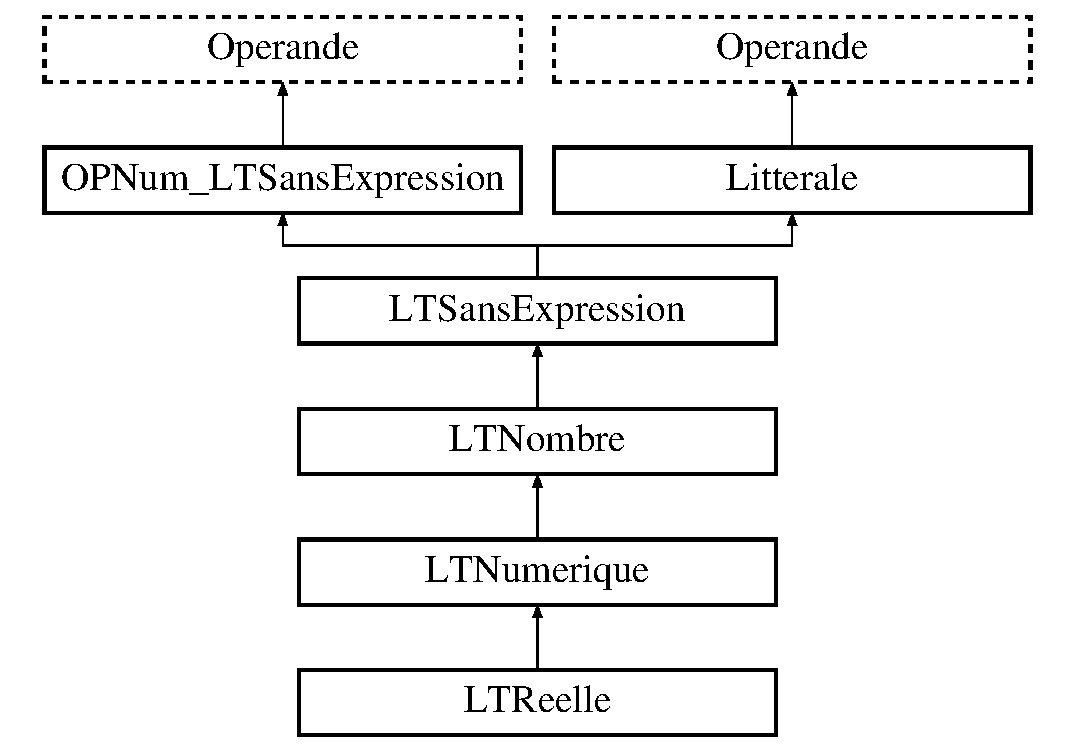
\includegraphics[height=6.000000cm]{class_l_t_reelle}
\end{center}
\end{figure}
\subsection*{Public Member Functions}
\begin{DoxyCompactItemize}
\item 
{\bfseries L\+T\+Reelle} (float v, \hyperlink{class_l_t_atome}{L\+T\+Atome} $\ast$a=0)\hypertarget{class_l_t_reelle_afb7cdbfe12872e93e79bac2966885e4e}{}\label{class_l_t_reelle_afb7cdbfe12872e93e79bac2966885e4e}

\item 
{\bfseries L\+T\+Reelle} (Q\+String v, \hyperlink{class_l_t_atome}{L\+T\+Atome} $\ast$a=0)\hypertarget{class_l_t_reelle_a470002c809b5589328d5f418e3807bc4}{}\label{class_l_t_reelle_a470002c809b5589328d5f418e3807bc4}

\item 
{\bfseries L\+T\+Reelle} (\hyperlink{class_l_t_rationnelle}{L\+T\+Rationnelle} $\ast$r)\hypertarget{class_l_t_reelle_aa939da3e27c0e5ee34bacd81eff0fa25}{}\label{class_l_t_reelle_aa939da3e27c0e5ee34bacd81eff0fa25}

\item 
{\bfseries L\+T\+Reelle} (const \hyperlink{class_l_t_reelle}{L\+T\+Reelle} \&r, \hyperlink{class_l_t_atome}{L\+T\+Atome} $\ast$a=0)\hypertarget{class_l_t_reelle_a4538afbd0564da09cbdc00a79786ec71}{}\label{class_l_t_reelle_a4538afbd0564da09cbdc00a79786ec71}

\item 
{\bfseries L\+T\+Reelle} (const \hyperlink{class_l_t_entier}{L\+T\+Entier} \&r, \hyperlink{class_l_t_atome}{L\+T\+Atome} $\ast$a=0)\hypertarget{class_l_t_reelle_abd48670d357c40e0a0035f08f8e20a59}{}\label{class_l_t_reelle_abd48670d357c40e0a0035f08f8e20a59}

\item 
float {\bfseries get\+Value} () const \hypertarget{class_l_t_reelle_adeeda9517c7e6194fdcb01f1be859591}{}\label{class_l_t_reelle_adeeda9517c7e6194fdcb01f1be859591}

\item 
void {\bfseries set\+Value} (float v)\hypertarget{class_l_t_reelle_a8ffcb74ee3e21f2389f274f953f7639d}{}\label{class_l_t_reelle_a8ffcb74ee3e21f2389f274f953f7639d}

\item 
void {\bfseries set\+Value} (Q\+String v)\hypertarget{class_l_t_reelle_a8fb7fee3b060e3e32af6f70bf7e11cf2}{}\label{class_l_t_reelle_a8fb7fee3b060e3e32af6f70bf7e11cf2}

\item 
int {\bfseries get\+E1} () const \hypertarget{class_l_t_reelle_aadc6331a7e20de9727f219f161c626a7}{}\label{class_l_t_reelle_aadc6331a7e20de9727f219f161c626a7}

\item 
float {\bfseries get\+E2} () const \hypertarget{class_l_t_reelle_a300d728fa9ca1fb3d1db086810339c21}{}\label{class_l_t_reelle_a300d728fa9ca1fb3d1db086810339c21}

\item 
virtual void \hyperlink{class_l_t_reelle_afed5ec07f74ea2ad2390d0dd11bee68f}{afficher} () const \hypertarget{class_l_t_reelle_afed5ec07f74ea2ad2390d0dd11bee68f}{}\label{class_l_t_reelle_afed5ec07f74ea2ad2390d0dd11bee68f}

\begin{DoxyCompactList}\small\item\em Fonction virtuelle affichant la litterale sur la sortie standart. \end{DoxyCompactList}\item 
virtual Q\+String \hyperlink{class_l_t_reelle_aa85d99c6c692e3fd51019630cfd88cc4}{get\+Text} () const 
\begin{DoxyCompactList}\small\item\em Fonction virtuelle renvoyant la litterale sous forme de texte. \end{DoxyCompactList}\item 
virtual \hyperlink{class_l_t_reelle}{L\+T\+Reelle} $\ast$ \hyperlink{class_l_t_reelle_a1dac7c02dfa84815730d5f0396ef1519}{clone} () const 
\begin{DoxyCompactList}\small\item\em Fonction virtuelle renvoyant une copie de l\textquotesingle{}instance. \end{DoxyCompactList}\item 
virtual \hyperlink{class_l_t_numerique}{L\+T\+Numerique} $\ast$ \hyperlink{class_l_t_reelle_aaaf23323d16d13b2ec7595c6aa07935f}{simplifier} ()
\begin{DoxyCompactList}\small\item\em Fonction virtuelle simplifiant la litterale actuelle. \end{DoxyCompactList}\item 
virtual \hyperlink{class_l_t_reelle}{L\+T\+Reelle} $\ast$ {\bfseries operator-\/-\/} ()\hypertarget{class_l_t_reelle_a8e72afe3c802aed84d10f7d32e794931}{}\label{class_l_t_reelle_a8e72afe3c802aed84d10f7d32e794931}

\item 
virtual \hyperlink{class_l_t_numerique}{L\+T\+Numerique} $\ast$ \hyperlink{class_l_t_reelle_a89bf36d07622d65ef879f8fbf14ffb88}{operator+} (\hyperlink{class_l_t_numerique}{L\+T\+Numerique} $\ast$p)
\begin{DoxyCompactList}\small\item\em Addition entre un \hyperlink{class_l_t_complexe}{L\+T\+Complexe} et un \hyperlink{class_l_t_numerique}{L\+T\+Numerique}. \end{DoxyCompactList}\item 
virtual \hyperlink{class_l_t_complexe}{L\+T\+Complexe} $\ast$ \hyperlink{class_l_t_reelle_af860cce772e4228c2a41654a074278c9}{operator+} (\hyperlink{class_l_t_complexe}{L\+T\+Complexe} $\ast$p)
\begin{DoxyCompactList}\small\item\em Addition entre un \hyperlink{class_l_t_complexe}{L\+T\+Complexe} et un \hyperlink{class_l_t_complexe}{L\+T\+Complexe}. \end{DoxyCompactList}\item 
virtual \hyperlink{class_l_t_numerique}{L\+T\+Numerique} $\ast$ \hyperlink{class_l_t_reelle_ab531e728f5055d41887f590db44ac4d2}{operator-\/} (\hyperlink{class_l_t_numerique}{L\+T\+Numerique} $\ast$p)
\begin{DoxyCompactList}\small\item\em Soustraction entre un \hyperlink{class_l_t_complexe}{L\+T\+Complexe} et un \hyperlink{class_l_t_numerique}{L\+T\+Numerique}. \end{DoxyCompactList}\item 
virtual \hyperlink{class_l_t_complexe}{L\+T\+Complexe} $\ast$ \hyperlink{class_l_t_reelle_a8f23a1ce94f266ab5b406769a94e88fe}{operator-\/} (\hyperlink{class_l_t_complexe}{L\+T\+Complexe} $\ast$p)
\begin{DoxyCompactList}\small\item\em Soustraction entre un \hyperlink{class_l_t_complexe}{L\+T\+Complexe} et un \hyperlink{class_l_t_complexe}{L\+T\+Complexe}. \end{DoxyCompactList}\item 
virtual \hyperlink{class_l_t_numerique}{L\+T\+Numerique} $\ast$ \hyperlink{class_l_t_reelle_a29fb03f19d56023485233168814c5f55}{operator$\ast$} (\hyperlink{class_l_t_numerique}{L\+T\+Numerique} $\ast$p)
\begin{DoxyCompactList}\small\item\em Multiplication entre un \hyperlink{class_l_t_complexe}{L\+T\+Complexe} et un \hyperlink{class_l_t_numerique}{L\+T\+Numerique}. \end{DoxyCompactList}\item 
virtual \hyperlink{class_l_t_complexe}{L\+T\+Complexe} $\ast$ \hyperlink{class_l_t_reelle_a6411ae704917972524001f81862814ff}{operator$\ast$} (\hyperlink{class_l_t_complexe}{L\+T\+Complexe} $\ast$p)
\begin{DoxyCompactList}\small\item\em Multiplication entre un \hyperlink{class_l_t_complexe}{L\+T\+Complexe} et un \hyperlink{class_l_t_complexe}{L\+T\+Complexe}. \end{DoxyCompactList}\item 
virtual \hyperlink{class_l_t_numerique}{L\+T\+Numerique} $\ast$ \hyperlink{class_l_t_reelle_a088c4683ed4077bceffca599f24fcee8}{operator/} (\hyperlink{class_l_t_numerique}{L\+T\+Numerique} $\ast$p)
\begin{DoxyCompactList}\small\item\em Division entre un \hyperlink{class_l_t_complexe}{L\+T\+Complexe} et un \hyperlink{class_l_t_numerique}{L\+T\+Numerique}. \end{DoxyCompactList}\item 
virtual \hyperlink{class_l_t_complexe}{L\+T\+Complexe} $\ast$ \hyperlink{class_l_t_reelle_a8260eb6ee9db3bea9798c49d1993060d}{operator/} (\hyperlink{class_l_t_complexe}{L\+T\+Complexe} $\ast$p)
\begin{DoxyCompactList}\small\item\em Division entre un \hyperlink{class_l_t_complexe}{L\+T\+Complexe} et un \hyperlink{class_l_t_numerique}{L\+T\+Numerique}. \end{DoxyCompactList}\end{DoxyCompactItemize}
\subsection*{Static Public Attributes}
\begin{DoxyCompactItemize}
\item 
static const \hyperlink{class_l_t_reelle}{L\+T\+Reelle} {\bfseries zero} = \hyperlink{class_l_t_reelle}{L\+T\+Reelle}(0.\+0)\hypertarget{class_l_t_reelle_af2b84064510c05ba009fa856d59d35f9}{}\label{class_l_t_reelle_af2b84064510c05ba009fa856d59d35f9}

\end{DoxyCompactItemize}
\subsection*{Friends}
\begin{DoxyCompactItemize}
\item 
bool {\bfseries operator==} (\hyperlink{class_l_t_reelle}{L\+T\+Reelle} \&l1, \hyperlink{class_l_t_reelle}{L\+T\+Reelle} \&l2)\hypertarget{class_l_t_reelle_a92e66f912fc575a5d2155d8c6dc7873d}{}\label{class_l_t_reelle_a92e66f912fc575a5d2155d8c6dc7873d}

\item 
bool {\bfseries operator==} (\hyperlink{class_l_t_reelle}{L\+T\+Reelle} \&l1, \hyperlink{class_l_t_rationnelle}{L\+T\+Rationnelle} \&l2)\hypertarget{class_l_t_reelle_a4cd73d7c2ae384207b1d83547277485a}{}\label{class_l_t_reelle_a4cd73d7c2ae384207b1d83547277485a}

\item 
bool {\bfseries operator==} (\hyperlink{class_l_t_reelle}{L\+T\+Reelle} \&l1, \hyperlink{class_l_t_entier}{L\+T\+Entier} \&l2)\hypertarget{class_l_t_reelle_a2512015bfd2ede84ea38cd9abddd0e33}{}\label{class_l_t_reelle_a2512015bfd2ede84ea38cd9abddd0e33}

\item 
bool {\bfseries operator$<$} (\hyperlink{class_l_t_reelle}{L\+T\+Reelle} \&l1, \hyperlink{class_l_t_reelle}{L\+T\+Reelle} \&l2)\hypertarget{class_l_t_reelle_a46fe306cc5831901d5602717c235df28}{}\label{class_l_t_reelle_a46fe306cc5831901d5602717c235df28}

\item 
bool {\bfseries operator$<$} (\hyperlink{class_l_t_reelle}{L\+T\+Reelle} \&l1, \hyperlink{class_l_t_rationnelle}{L\+T\+Rationnelle} \&l2)\hypertarget{class_l_t_reelle_a902969226cb6b6cb2baf1e6f90703b53}{}\label{class_l_t_reelle_a902969226cb6b6cb2baf1e6f90703b53}

\item 
bool {\bfseries operator$<$} (\hyperlink{class_l_t_reelle}{L\+T\+Reelle} \&l1, \hyperlink{class_l_t_entier}{L\+T\+Entier} \&l2)\hypertarget{class_l_t_reelle_a36370861ff6512aa9e655ef7449df180}{}\label{class_l_t_reelle_a36370861ff6512aa9e655ef7449df180}

\end{DoxyCompactItemize}
\subsection*{Additional Inherited Members}


\subsection{Member Function Documentation}
\index{L\+T\+Reelle@{L\+T\+Reelle}!clone@{clone}}
\index{clone@{clone}!L\+T\+Reelle@{L\+T\+Reelle}}
\subsubsection[{\texorpdfstring{clone() const }{clone() const }}]{\setlength{\rightskip}{0pt plus 5cm}{\bf L\+T\+Reelle} $\ast$ L\+T\+Reelle\+::clone (
\begin{DoxyParamCaption}
{}
\end{DoxyParamCaption}
) const\hspace{0.3cm}{\ttfamily [virtual]}}\hypertarget{class_l_t_reelle_a1dac7c02dfa84815730d5f0396ef1519}{}\label{class_l_t_reelle_a1dac7c02dfa84815730d5f0396ef1519}


Fonction virtuelle renvoyant une copie de l\textquotesingle{}instance. 

\begin{DoxyReturn}{Returns}
Nouvelle litterale copiée 
\end{DoxyReturn}


Implements \hyperlink{class_l_t_numerique_a884056443dd30cd71c49b42b5ba63581}{L\+T\+Numerique}.

\index{L\+T\+Reelle@{L\+T\+Reelle}!get\+Text@{get\+Text}}
\index{get\+Text@{get\+Text}!L\+T\+Reelle@{L\+T\+Reelle}}
\subsubsection[{\texorpdfstring{get\+Text() const }{getText() const }}]{\setlength{\rightskip}{0pt plus 5cm}Q\+String L\+T\+Reelle\+::get\+Text (
\begin{DoxyParamCaption}
{}
\end{DoxyParamCaption}
) const\hspace{0.3cm}{\ttfamily [virtual]}}\hypertarget{class_l_t_reelle_aa85d99c6c692e3fd51019630cfd88cc4}{}\label{class_l_t_reelle_aa85d99c6c692e3fd51019630cfd88cc4}


Fonction virtuelle renvoyant la litterale sous forme de texte. 

\begin{DoxyReturn}{Returns}
\hyperlink{class_litterale}{Litterale} sous forme de texte 
\end{DoxyReturn}


Implements \hyperlink{class_l_t_numerique_abef28b1b62ee356717f70f4317a44590}{L\+T\+Numerique}.

\index{L\+T\+Reelle@{L\+T\+Reelle}!operator$\ast$@{operator$\ast$}}
\index{operator$\ast$@{operator$\ast$}!L\+T\+Reelle@{L\+T\+Reelle}}
\subsubsection[{\texorpdfstring{operator$\ast$(\+L\+T\+Numerique $\ast$p)}{operator*(LTNumerique *p)}}]{\setlength{\rightskip}{0pt plus 5cm}{\bf L\+T\+Numerique} $\ast$ L\+T\+Reelle\+::operator$\ast$ (
\begin{DoxyParamCaption}
\item[{{\bf L\+T\+Numerique} $\ast$}]{p}
\end{DoxyParamCaption}
)\hspace{0.3cm}{\ttfamily [virtual]}}\hypertarget{class_l_t_reelle_a29fb03f19d56023485233168814c5f55}{}\label{class_l_t_reelle_a29fb03f19d56023485233168814c5f55}


Multiplication entre un \hyperlink{class_l_t_complexe}{L\+T\+Complexe} et un \hyperlink{class_l_t_numerique}{L\+T\+Numerique}. 


\begin{DoxyParams}{Parameters}
{\em p} & Variable à ajouter \\
\hline
\end{DoxyParams}
\begin{DoxyReturn}{Returns}
\hyperlink{class_l_t_nombre}{L\+T\+Nombre} créé 
\end{DoxyReturn}


Implements \hyperlink{class_l_t_numerique_aef374b7679c6b9b7901e0a4bbfce4cc3}{L\+T\+Numerique}.

\index{L\+T\+Reelle@{L\+T\+Reelle}!operator$\ast$@{operator$\ast$}}
\index{operator$\ast$@{operator$\ast$}!L\+T\+Reelle@{L\+T\+Reelle}}
\subsubsection[{\texorpdfstring{operator$\ast$(\+L\+T\+Complexe $\ast$p)}{operator*(LTComplexe *p)}}]{\setlength{\rightskip}{0pt plus 5cm}{\bf L\+T\+Complexe} $\ast$ L\+T\+Reelle\+::operator$\ast$ (
\begin{DoxyParamCaption}
\item[{{\bf L\+T\+Complexe} $\ast$}]{p}
\end{DoxyParamCaption}
)\hspace{0.3cm}{\ttfamily [virtual]}}\hypertarget{class_l_t_reelle_a6411ae704917972524001f81862814ff}{}\label{class_l_t_reelle_a6411ae704917972524001f81862814ff}


Multiplication entre un \hyperlink{class_l_t_complexe}{L\+T\+Complexe} et un \hyperlink{class_l_t_complexe}{L\+T\+Complexe}. 


\begin{DoxyParams}{Parameters}
{\em p} & Variable à ajouter \\
\hline
\end{DoxyParams}
\begin{DoxyReturn}{Returns}
\hyperlink{class_l_t_complexe}{L\+T\+Complexe} créé 
\end{DoxyReturn}


Implements \hyperlink{class_l_t_numerique_a6991c6c854915c7bfd98634c791ab815}{L\+T\+Numerique}.

\index{L\+T\+Reelle@{L\+T\+Reelle}!operator+@{operator+}}
\index{operator+@{operator+}!L\+T\+Reelle@{L\+T\+Reelle}}
\subsubsection[{\texorpdfstring{operator+(\+L\+T\+Numerique $\ast$p)}{operator+(LTNumerique *p)}}]{\setlength{\rightskip}{0pt plus 5cm}{\bf L\+T\+Numerique} $\ast$ L\+T\+Reelle\+::operator+ (
\begin{DoxyParamCaption}
\item[{{\bf L\+T\+Numerique} $\ast$}]{p}
\end{DoxyParamCaption}
)\hspace{0.3cm}{\ttfamily [virtual]}}\hypertarget{class_l_t_reelle_a89bf36d07622d65ef879f8fbf14ffb88}{}\label{class_l_t_reelle_a89bf36d07622d65ef879f8fbf14ffb88}


Addition entre un \hyperlink{class_l_t_complexe}{L\+T\+Complexe} et un \hyperlink{class_l_t_numerique}{L\+T\+Numerique}. 


\begin{DoxyParams}{Parameters}
{\em p} & Variable à ajouter \\
\hline
\end{DoxyParams}
\begin{DoxyReturn}{Returns}
\hyperlink{class_l_t_nombre}{L\+T\+Nombre} créé 
\end{DoxyReturn}


Implements \hyperlink{class_l_t_numerique_a9fb09223dc517fae452f4af0d50f6966}{L\+T\+Numerique}.

\index{L\+T\+Reelle@{L\+T\+Reelle}!operator+@{operator+}}
\index{operator+@{operator+}!L\+T\+Reelle@{L\+T\+Reelle}}
\subsubsection[{\texorpdfstring{operator+(\+L\+T\+Complexe $\ast$p)}{operator+(LTComplexe *p)}}]{\setlength{\rightskip}{0pt plus 5cm}{\bf L\+T\+Complexe} $\ast$ L\+T\+Reelle\+::operator+ (
\begin{DoxyParamCaption}
\item[{{\bf L\+T\+Complexe} $\ast$}]{p}
\end{DoxyParamCaption}
)\hspace{0.3cm}{\ttfamily [virtual]}}\hypertarget{class_l_t_reelle_af860cce772e4228c2a41654a074278c9}{}\label{class_l_t_reelle_af860cce772e4228c2a41654a074278c9}


Addition entre un \hyperlink{class_l_t_complexe}{L\+T\+Complexe} et un \hyperlink{class_l_t_complexe}{L\+T\+Complexe}. 


\begin{DoxyParams}{Parameters}
{\em p} & Variable à ajouter \\
\hline
\end{DoxyParams}
\begin{DoxyReturn}{Returns}
\hyperlink{class_l_t_complexe}{L\+T\+Complexe} créé 
\end{DoxyReturn}


Implements \hyperlink{class_l_t_numerique_a615173a7cd77e649235d1c06d72726e7}{L\+T\+Numerique}.

\index{L\+T\+Reelle@{L\+T\+Reelle}!operator-\/@{operator-\/}}
\index{operator-\/@{operator-\/}!L\+T\+Reelle@{L\+T\+Reelle}}
\subsubsection[{\texorpdfstring{operator-\/(\+L\+T\+Numerique $\ast$p)}{operator-(LTNumerique *p)}}]{\setlength{\rightskip}{0pt plus 5cm}{\bf L\+T\+Numerique} $\ast$ L\+T\+Reelle\+::operator-\/ (
\begin{DoxyParamCaption}
\item[{{\bf L\+T\+Numerique} $\ast$}]{p}
\end{DoxyParamCaption}
)\hspace{0.3cm}{\ttfamily [virtual]}}\hypertarget{class_l_t_reelle_ab531e728f5055d41887f590db44ac4d2}{}\label{class_l_t_reelle_ab531e728f5055d41887f590db44ac4d2}


Soustraction entre un \hyperlink{class_l_t_complexe}{L\+T\+Complexe} et un \hyperlink{class_l_t_numerique}{L\+T\+Numerique}. 


\begin{DoxyParams}{Parameters}
{\em p} & Variable à ajouter \\
\hline
\end{DoxyParams}
\begin{DoxyReturn}{Returns}
\hyperlink{class_l_t_nombre}{L\+T\+Nombre} créé 
\end{DoxyReturn}


Implements \hyperlink{class_l_t_numerique_a94d98eef8d391bdb925dbb70a1b35834}{L\+T\+Numerique}.

\index{L\+T\+Reelle@{L\+T\+Reelle}!operator-\/@{operator-\/}}
\index{operator-\/@{operator-\/}!L\+T\+Reelle@{L\+T\+Reelle}}
\subsubsection[{\texorpdfstring{operator-\/(\+L\+T\+Complexe $\ast$p)}{operator-(LTComplexe *p)}}]{\setlength{\rightskip}{0pt plus 5cm}{\bf L\+T\+Complexe} $\ast$ L\+T\+Reelle\+::operator-\/ (
\begin{DoxyParamCaption}
\item[{{\bf L\+T\+Complexe} $\ast$}]{p}
\end{DoxyParamCaption}
)\hspace{0.3cm}{\ttfamily [virtual]}}\hypertarget{class_l_t_reelle_a8f23a1ce94f266ab5b406769a94e88fe}{}\label{class_l_t_reelle_a8f23a1ce94f266ab5b406769a94e88fe}


Soustraction entre un \hyperlink{class_l_t_complexe}{L\+T\+Complexe} et un \hyperlink{class_l_t_complexe}{L\+T\+Complexe}. 


\begin{DoxyParams}{Parameters}
{\em p} & Variable à ajouter \\
\hline
\end{DoxyParams}
\begin{DoxyReturn}{Returns}
\hyperlink{class_l_t_complexe}{L\+T\+Complexe} créé 
\end{DoxyReturn}


Implements \hyperlink{class_l_t_numerique_a45bbf62a5725c3b9c8a8a14d9be6ef47}{L\+T\+Numerique}.

\index{L\+T\+Reelle@{L\+T\+Reelle}!operator/@{operator/}}
\index{operator/@{operator/}!L\+T\+Reelle@{L\+T\+Reelle}}
\subsubsection[{\texorpdfstring{operator/(\+L\+T\+Numerique $\ast$p)}{operator/(LTNumerique *p)}}]{\setlength{\rightskip}{0pt plus 5cm}{\bf L\+T\+Numerique} $\ast$ L\+T\+Reelle\+::operator/ (
\begin{DoxyParamCaption}
\item[{{\bf L\+T\+Numerique} $\ast$}]{p}
\end{DoxyParamCaption}
)\hspace{0.3cm}{\ttfamily [virtual]}}\hypertarget{class_l_t_reelle_a088c4683ed4077bceffca599f24fcee8}{}\label{class_l_t_reelle_a088c4683ed4077bceffca599f24fcee8}


Division entre un \hyperlink{class_l_t_complexe}{L\+T\+Complexe} et un \hyperlink{class_l_t_numerique}{L\+T\+Numerique}. 


\begin{DoxyParams}{Parameters}
{\em p} & Variable à ajouter \\
\hline
\end{DoxyParams}
\begin{DoxyReturn}{Returns}
\hyperlink{class_l_t_nombre}{L\+T\+Nombre} créé 
\end{DoxyReturn}


Implements \hyperlink{class_l_t_numerique_ab3acc500e7c92b2d1e05ebc65561b84a}{L\+T\+Numerique}.

\index{L\+T\+Reelle@{L\+T\+Reelle}!operator/@{operator/}}
\index{operator/@{operator/}!L\+T\+Reelle@{L\+T\+Reelle}}
\subsubsection[{\texorpdfstring{operator/(\+L\+T\+Complexe $\ast$p)}{operator/(LTComplexe *p)}}]{\setlength{\rightskip}{0pt plus 5cm}{\bf L\+T\+Complexe} $\ast$ L\+T\+Reelle\+::operator/ (
\begin{DoxyParamCaption}
\item[{{\bf L\+T\+Complexe} $\ast$}]{p}
\end{DoxyParamCaption}
)\hspace{0.3cm}{\ttfamily [virtual]}}\hypertarget{class_l_t_reelle_a8260eb6ee9db3bea9798c49d1993060d}{}\label{class_l_t_reelle_a8260eb6ee9db3bea9798c49d1993060d}


Division entre un \hyperlink{class_l_t_complexe}{L\+T\+Complexe} et un \hyperlink{class_l_t_numerique}{L\+T\+Numerique}. 


\begin{DoxyParams}{Parameters}
{\em p} & Variable à ajouter \\
\hline
\end{DoxyParams}
\begin{DoxyReturn}{Returns}
\hyperlink{class_l_t_complexe}{L\+T\+Complexe} créé 
\end{DoxyReturn}


Implements \hyperlink{class_l_t_numerique_a223402e5b15e25f716bdd1981f59f39d}{L\+T\+Numerique}.

\index{L\+T\+Reelle@{L\+T\+Reelle}!simplifier@{simplifier}}
\index{simplifier@{simplifier}!L\+T\+Reelle@{L\+T\+Reelle}}
\subsubsection[{\texorpdfstring{simplifier()}{simplifier()}}]{\setlength{\rightskip}{0pt plus 5cm}virtual {\bf L\+T\+Numerique}$\ast$ L\+T\+Reelle\+::simplifier (
\begin{DoxyParamCaption}
{}
\end{DoxyParamCaption}
)\hspace{0.3cm}{\ttfamily [inline]}, {\ttfamily [virtual]}}\hypertarget{class_l_t_reelle_aaaf23323d16d13b2ec7595c6aa07935f}{}\label{class_l_t_reelle_aaaf23323d16d13b2ec7595c6aa07935f}


Fonction virtuelle simplifiant la litterale actuelle. 

\begin{DoxyReturn}{Returns}
Nouvelle litterale copiée 
\end{DoxyReturn}


Implements \hyperlink{class_l_t_numerique_a3963de62916188d01f93b1d0fdb42c7f}{L\+T\+Numerique}.



The documentation for this class was generated from the following files\+:\begin{DoxyCompactItemize}
\item 
ltnumerique.\+h\item 
ltnumerique.\+cpp\end{DoxyCompactItemize}

\hypertarget{class_l_t_sans_expression}{}\section{L\+T\+Sans\+Expression Class Reference}
\label{class_l_t_sans_expression}\index{L\+T\+Sans\+Expression@{L\+T\+Sans\+Expression}}
Inheritance diagram for L\+T\+Sans\+Expression\+:\begin{figure}[H]
\begin{center}
\leavevmode
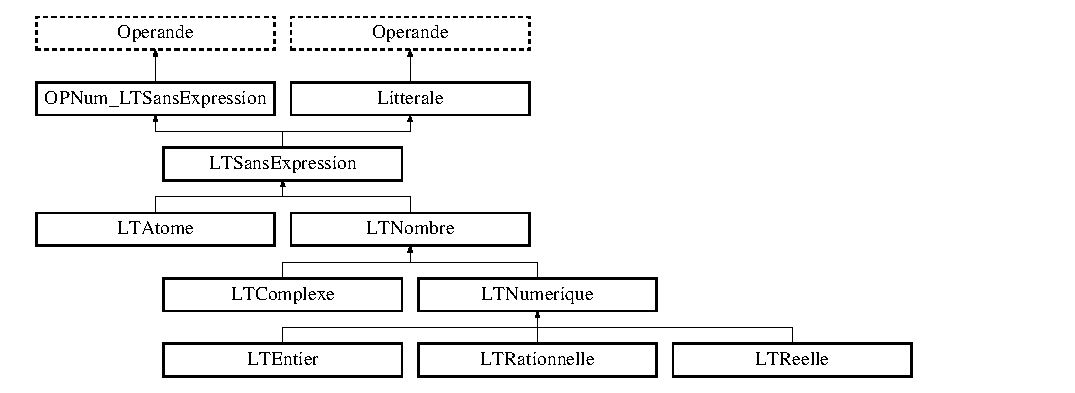
\includegraphics[height=4.827586cm]{class_l_t_sans_expression}
\end{center}
\end{figure}
\subsection*{Public Member Functions}
\begin{DoxyCompactItemize}
\item 
virtual Q\+String \hyperlink{class_l_t_sans_expression_a4f0372c490b49bfc654e394a59c4c015}{get\+Text} () const  =0
\begin{DoxyCompactList}\small\item\em Fonction virtuelle renvoyant la litterale sous forme de texte. \end{DoxyCompactList}\item 
virtual void \hyperlink{class_l_t_sans_expression_a7dfd1943b7db32d9e4f35eaaec49ad0d}{afficher} () const  =0\hypertarget{class_l_t_sans_expression_a7dfd1943b7db32d9e4f35eaaec49ad0d}{}\label{class_l_t_sans_expression_a7dfd1943b7db32d9e4f35eaaec49ad0d}

\begin{DoxyCompactList}\small\item\em Fonction virtuelle affichant la litterale sur la sortie standart. \end{DoxyCompactList}\item 
virtual \hyperlink{class_l_t_sans_expression}{L\+T\+Sans\+Expression} $\ast$ \hyperlink{class_l_t_sans_expression_af0299c947bb7a910ddd4c419cf729313}{clone} () const  =0
\begin{DoxyCompactList}\small\item\em Fonction virtuelle renvoyant une copie de l\textquotesingle{}instance. \end{DoxyCompactList}\item 
virtual \hyperlink{class_litterale}{Litterale} $\ast$ \hyperlink{class_l_t_sans_expression_a13982a6a4f155bac50a0058a2c352e91}{simplifier} ()=0
\begin{DoxyCompactList}\small\item\em Fonction virtuelle simplifiant la litterale actuelle. \end{DoxyCompactList}\end{DoxyCompactItemize}


\subsection{Member Function Documentation}
\index{L\+T\+Sans\+Expression@{L\+T\+Sans\+Expression}!clone@{clone}}
\index{clone@{clone}!L\+T\+Sans\+Expression@{L\+T\+Sans\+Expression}}
\subsubsection[{\texorpdfstring{clone() const  =0}{clone() const  =0}}]{\setlength{\rightskip}{0pt plus 5cm}virtual {\bf L\+T\+Sans\+Expression}$\ast$ L\+T\+Sans\+Expression\+::clone (
\begin{DoxyParamCaption}
{}
\end{DoxyParamCaption}
) const\hspace{0.3cm}{\ttfamily [pure virtual]}}\hypertarget{class_l_t_sans_expression_af0299c947bb7a910ddd4c419cf729313}{}\label{class_l_t_sans_expression_af0299c947bb7a910ddd4c419cf729313}


Fonction virtuelle renvoyant une copie de l\textquotesingle{}instance. 

\begin{DoxyReturn}{Returns}
Nouvelle litterale copiée 
\end{DoxyReturn}


Implements \hyperlink{class_litterale_a08967178d22c3d69e6c3e86ea8c85888}{Litterale}.



Implemented in \hyperlink{class_l_t_reelle_a1dac7c02dfa84815730d5f0396ef1519}{L\+T\+Reelle}, \hyperlink{class_l_t_rationnelle_a48b36c50460ce15674d1d72afb41daf3}{L\+T\+Rationnelle}, \hyperlink{class_l_t_entier_afc21b025efd3feea0162053902b8d640}{L\+T\+Entier}, \hyperlink{class_l_t_atome_a8fd75a87781e2544fb090da6096a7106}{L\+T\+Atome}, \hyperlink{class_l_t_complexe_ae597257b1e7b81ad6914e44b616c006d}{L\+T\+Complexe}, \hyperlink{class_l_t_numerique_a884056443dd30cd71c49b42b5ba63581}{L\+T\+Numerique}, and \hyperlink{class_l_t_nombre_a09ad6faddbb007746e41af6873bd1824}{L\+T\+Nombre}.

\index{L\+T\+Sans\+Expression@{L\+T\+Sans\+Expression}!get\+Text@{get\+Text}}
\index{get\+Text@{get\+Text}!L\+T\+Sans\+Expression@{L\+T\+Sans\+Expression}}
\subsubsection[{\texorpdfstring{get\+Text() const  =0}{getText() const  =0}}]{\setlength{\rightskip}{0pt plus 5cm}virtual Q\+String L\+T\+Sans\+Expression\+::get\+Text (
\begin{DoxyParamCaption}
{}
\end{DoxyParamCaption}
) const\hspace{0.3cm}{\ttfamily [pure virtual]}}\hypertarget{class_l_t_sans_expression_a4f0372c490b49bfc654e394a59c4c015}{}\label{class_l_t_sans_expression_a4f0372c490b49bfc654e394a59c4c015}


Fonction virtuelle renvoyant la litterale sous forme de texte. 

\begin{DoxyReturn}{Returns}
\hyperlink{class_litterale}{Litterale} sous forme de texte 
\end{DoxyReturn}


Implements \hyperlink{class_litterale_a780075c00abf31efb87e7c28843ea029}{Litterale}.



Implemented in \hyperlink{class_l_t_reelle_aa85d99c6c692e3fd51019630cfd88cc4}{L\+T\+Reelle}, \hyperlink{class_l_t_rationnelle_a7195f7e7ddfe6c5493932fe08785ac76}{L\+T\+Rationnelle}, \hyperlink{class_l_t_entier_a735c05de25b1264a5b2bc603f63eed58}{L\+T\+Entier}, \hyperlink{class_l_t_atome_a2140a7071f7d1d5ddca671802de17447}{L\+T\+Atome}, \hyperlink{class_l_t_complexe_a25992476892bbc3a33ea61dba8bc9160}{L\+T\+Complexe}, \hyperlink{class_l_t_numerique_abef28b1b62ee356717f70f4317a44590}{L\+T\+Numerique}, and \hyperlink{class_l_t_nombre_a39fe941ec69bf013bc3be8b3e575c3d0}{L\+T\+Nombre}.

\index{L\+T\+Sans\+Expression@{L\+T\+Sans\+Expression}!simplifier@{simplifier}}
\index{simplifier@{simplifier}!L\+T\+Sans\+Expression@{L\+T\+Sans\+Expression}}
\subsubsection[{\texorpdfstring{simplifier()=0}{simplifier()=0}}]{\setlength{\rightskip}{0pt plus 5cm}virtual {\bf Litterale}$\ast$ L\+T\+Sans\+Expression\+::simplifier (
\begin{DoxyParamCaption}
{}
\end{DoxyParamCaption}
)\hspace{0.3cm}{\ttfamily [pure virtual]}}\hypertarget{class_l_t_sans_expression_a13982a6a4f155bac50a0058a2c352e91}{}\label{class_l_t_sans_expression_a13982a6a4f155bac50a0058a2c352e91}


Fonction virtuelle simplifiant la litterale actuelle. 

\begin{DoxyReturn}{Returns}
Nouvelle litterale copiée 
\end{DoxyReturn}


Implements \hyperlink{class_litterale_af33a0c1a4a9a5bb687da112b12f0e6e6}{Litterale}.



Implemented in \hyperlink{class_l_t_reelle_aaaf23323d16d13b2ec7595c6aa07935f}{L\+T\+Reelle}, \hyperlink{class_l_t_rationnelle_afefcccb71e7fd20491e8f14aef88dd6e}{L\+T\+Rationnelle}, \hyperlink{class_l_t_entier_a3dd0959762240ef5cbe0a62970728ddf}{L\+T\+Entier}, \hyperlink{class_l_t_atome_a2e2cee64c687ab8c648e4866ab1150b8}{L\+T\+Atome}, \hyperlink{class_l_t_complexe_aa4781a2130c4dd2daa81fde8caa6fff3}{L\+T\+Complexe}, \hyperlink{class_l_t_numerique_a3963de62916188d01f93b1d0fdb42c7f}{L\+T\+Numerique}, and \hyperlink{class_l_t_nombre_a6aa1593c8c0956bb5412bfee3c15b085}{L\+T\+Nombre}.



The documentation for this class was generated from the following file\+:\begin{DoxyCompactItemize}
\item 
ltsansexpression.\+h\end{DoxyCompactItemize}

\hypertarget{class_memento}{}\section{Memento Class Reference}
\label{class_memento}\index{Memento@{Memento}}
\subsection*{Public Member Functions}
\begin{DoxyCompactItemize}
\item 
{\bfseries Memento} (\hyperlink{class_stack}{Stack} $\ast$s)\hypertarget{class_memento_a3f27270396c420ed09ac51a4cee5d129}{}\label{class_memento_a3f27270396c420ed09ac51a4cee5d129}

\item 
\hyperlink{class_stack}{Stack} $\ast$ {\bfseries get\+Stack} ()\hypertarget{class_memento_ae9ff6624ae6da087f1e05d17c579453a}{}\label{class_memento_ae9ff6624ae6da087f1e05d17c579453a}

\end{DoxyCompactItemize}


The documentation for this class was generated from the following file\+:\begin{DoxyCompactItemize}
\item 
memento.\+h\end{DoxyCompactItemize}

\hypertarget{class_o_p_addition}{}\section{O\+P\+Addition Class Reference}
\label{class_o_p_addition}\index{O\+P\+Addition@{O\+P\+Addition}}
Inheritance diagram for O\+P\+Addition\+:\begin{figure}[H]
\begin{center}
\leavevmode
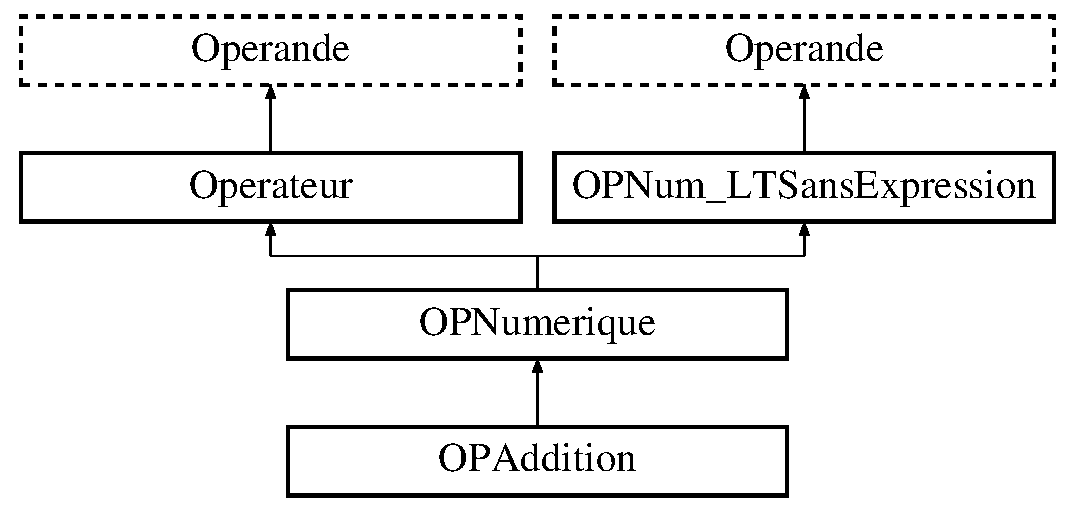
\includegraphics[height=4.000000cm]{class_o_p_addition}
\end{center}
\end{figure}
\subsection*{Public Member Functions}
\begin{DoxyCompactItemize}
\item 
virtual \hyperlink{class_o_p_addition}{O\+P\+Addition} $\ast$ {\bfseries clone} () const \hypertarget{class_o_p_addition_ab1d9b58d91b92f98e6c362630eddb9a9}{}\label{class_o_p_addition_ab1d9b58d91b92f98e6c362630eddb9a9}

\item 
virtual \hyperlink{class_litterale}{Litterale} $\ast$ {\bfseries compute} ()\hypertarget{class_o_p_addition_a55b0a7e511f20228d3ed360e6e50efa6}{}\label{class_o_p_addition_a55b0a7e511f20228d3ed360e6e50efa6}

\item 
virtual \hyperlink{class_litterale}{Litterale} $\ast$ {\bfseries compute} (\hyperlink{class_litterale}{Litterale} $\ast$l)\hypertarget{class_o_p_addition_ae700f6d3003aff66ac2972ff8b1a6398}{}\label{class_o_p_addition_ae700f6d3003aff66ac2972ff8b1a6398}

\item 
virtual \hyperlink{class_litterale}{Litterale} $\ast$ {\bfseries compute} (\hyperlink{class_litterale}{Litterale} $\ast$l1, \hyperlink{class_litterale}{Litterale} $\ast$l2)\hypertarget{class_o_p_addition_a37b7577267559130d0e7da6f4842e65a}{}\label{class_o_p_addition_a37b7577267559130d0e7da6f4842e65a}

\end{DoxyCompactItemize}
\subsection*{Additional Inherited Members}


The documentation for this class was generated from the following files\+:\begin{DoxyCompactItemize}
\item 
opnumerique.\+h\item 
opnumerique.\+cpp\end{DoxyCompactItemize}

\hypertarget{class_o_p_and}{}\section{O\+P\+And Class Reference}
\label{class_o_p_and}\index{O\+P\+And@{O\+P\+And}}
Inheritance diagram for O\+P\+And\+:\begin{figure}[H]
\begin{center}
\leavevmode
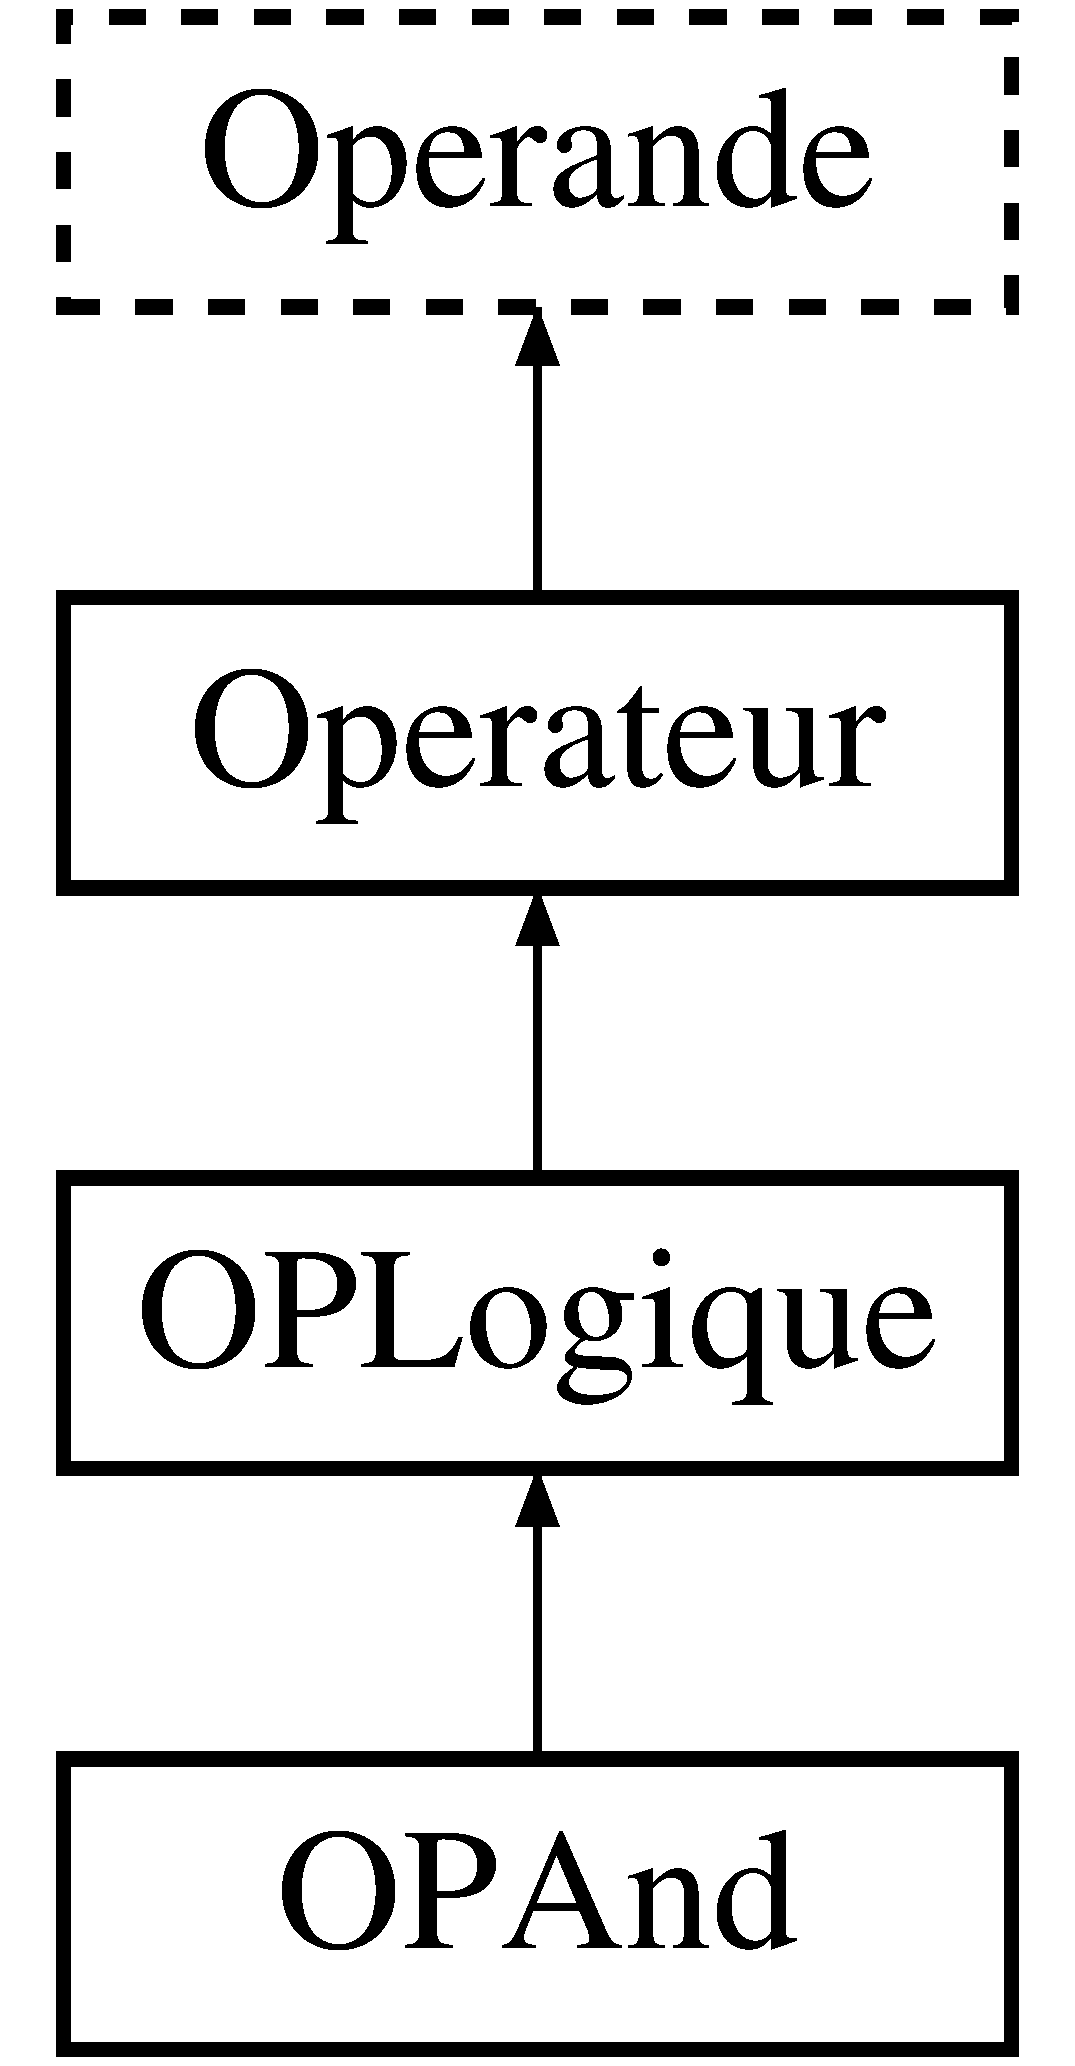
\includegraphics[height=4.000000cm]{class_o_p_and}
\end{center}
\end{figure}
\subsection*{Public Member Functions}
\begin{DoxyCompactItemize}
\item 
virtual \hyperlink{class_o_p_and}{O\+P\+And} $\ast$ {\bfseries clone} () const \hypertarget{class_o_p_and_ad31a372d9b3b021f64832cfb42c65b64}{}\label{class_o_p_and_ad31a372d9b3b021f64832cfb42c65b64}

\item 
virtual \hyperlink{class_litterale}{Litterale} $\ast$ {\bfseries compute} ()\hypertarget{class_o_p_and_acd2035cca02eead57283ed715e8de918}{}\label{class_o_p_and_acd2035cca02eead57283ed715e8de918}

\item 
virtual \hyperlink{class_litterale}{Litterale} $\ast$ {\bfseries compute} (\hyperlink{class_litterale}{Litterale} $\ast$l)\hypertarget{class_o_p_and_a4ae71086cefdc561d8e67ab7f8e094d9}{}\label{class_o_p_and_a4ae71086cefdc561d8e67ab7f8e094d9}

\item 
virtual \hyperlink{class_litterale}{Litterale} $\ast$ {\bfseries compute} (\hyperlink{class_litterale}{Litterale} $\ast$l1, \hyperlink{class_litterale}{Litterale} $\ast$l2)\hypertarget{class_o_p_and_a5cd30ba5edec5a8264a244507eb239eb}{}\label{class_o_p_and_a5cd30ba5edec5a8264a244507eb239eb}

\end{DoxyCompactItemize}
\subsection*{Additional Inherited Members}


The documentation for this class was generated from the following files\+:\begin{DoxyCompactItemize}
\item 
oplogique.\+h\item 
oplogique.\+cpp\end{DoxyCompactItemize}

\hypertarget{class_o_p_atome}{}\section{O\+P\+Atome Class Reference}
\label{class_o_p_atome}\index{O\+P\+Atome@{O\+P\+Atome}}
Inheritance diagram for O\+P\+Atome\+:\begin{figure}[H]
\begin{center}
\leavevmode
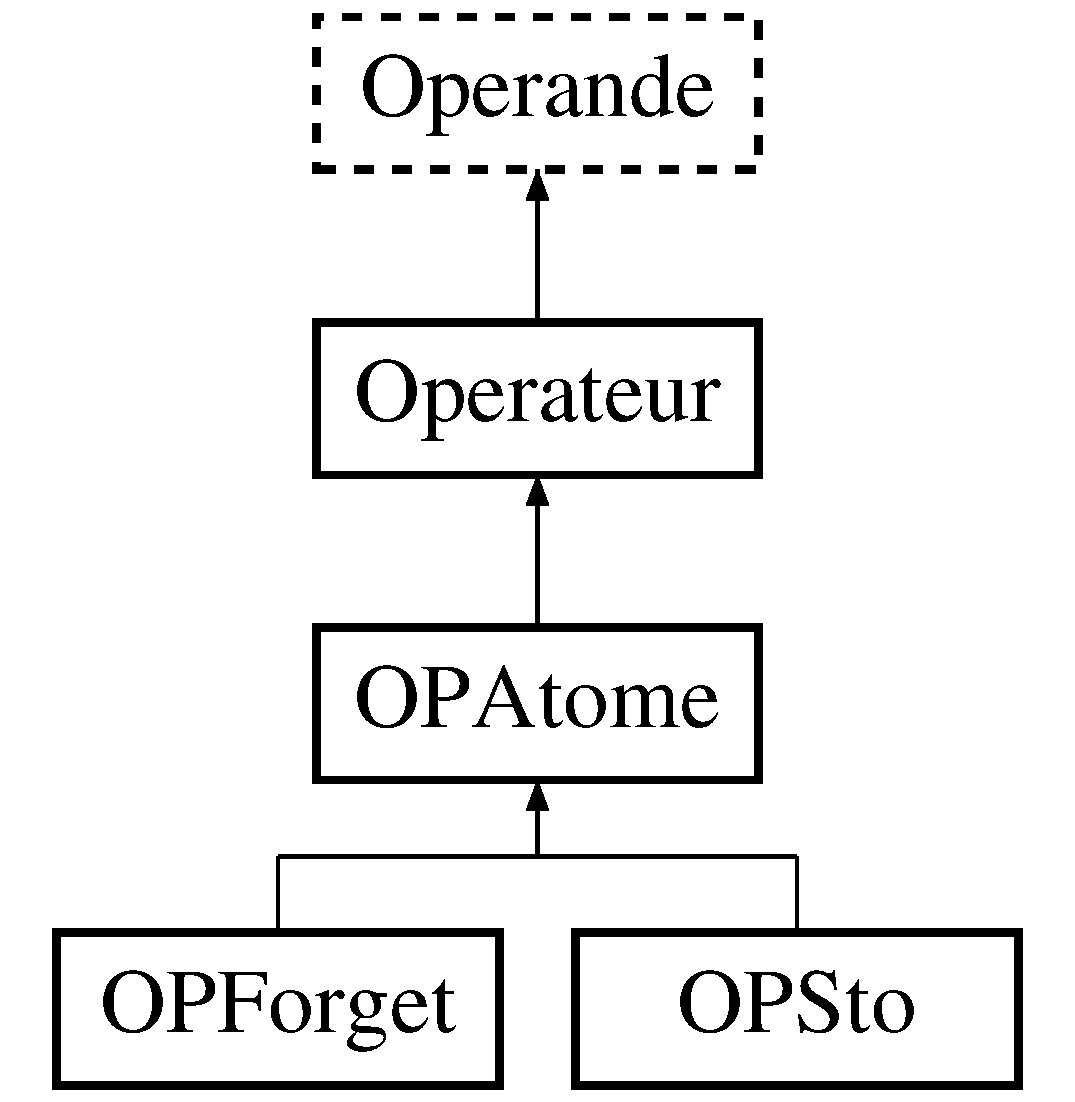
\includegraphics[height=4.000000cm]{class_o_p_atome}
\end{center}
\end{figure}
\subsection*{Public Member Functions}
\begin{DoxyCompactItemize}
\item 
{\bfseries O\+P\+Atome} (Q\+String val, int a)\hypertarget{class_o_p_atome_aa47784bcda6dab75a621d2d8e0dcbb78}{}\label{class_o_p_atome_aa47784bcda6dab75a621d2d8e0dcbb78}

\item 
virtual \hyperlink{class_o_p_atome}{O\+P\+Atome} $\ast$ {\bfseries clone} () const  =0\hypertarget{class_o_p_atome_a15ce92ba697325a96a37b35218266ae6}{}\label{class_o_p_atome_a15ce92ba697325a96a37b35218266ae6}

\item 
virtual \hyperlink{class_litterale}{Litterale} $\ast$ {\bfseries compute} ()=0\hypertarget{class_o_p_atome_a3251b1758ab0806376472ca8e93e6389}{}\label{class_o_p_atome_a3251b1758ab0806376472ca8e93e6389}

\item 
virtual \hyperlink{class_litterale}{Litterale} $\ast$ {\bfseries compute} (\hyperlink{class_litterale}{Litterale} $\ast$l)=0\hypertarget{class_o_p_atome_af3a80639cbea23c292c738650d0f7fa7}{}\label{class_o_p_atome_af3a80639cbea23c292c738650d0f7fa7}

\item 
virtual \hyperlink{class_litterale}{Litterale} $\ast$ {\bfseries compute} (\hyperlink{class_litterale}{Litterale} $\ast$l1, \hyperlink{class_litterale}{Litterale} $\ast$l2)=0\hypertarget{class_o_p_atome_ac610442d3bc2da08ed80698bcbd0e095}{}\label{class_o_p_atome_ac610442d3bc2da08ed80698bcbd0e095}

\end{DoxyCompactItemize}
\subsection*{Additional Inherited Members}


The documentation for this class was generated from the following file\+:\begin{DoxyCompactItemize}
\item 
opatome.\+h\end{DoxyCompactItemize}

\hypertarget{class_o_p_clear}{}\section{O\+P\+Clear Class Reference}
\label{class_o_p_clear}\index{O\+P\+Clear@{O\+P\+Clear}}
Inheritance diagram for O\+P\+Clear\+:\begin{figure}[H]
\begin{center}
\leavevmode
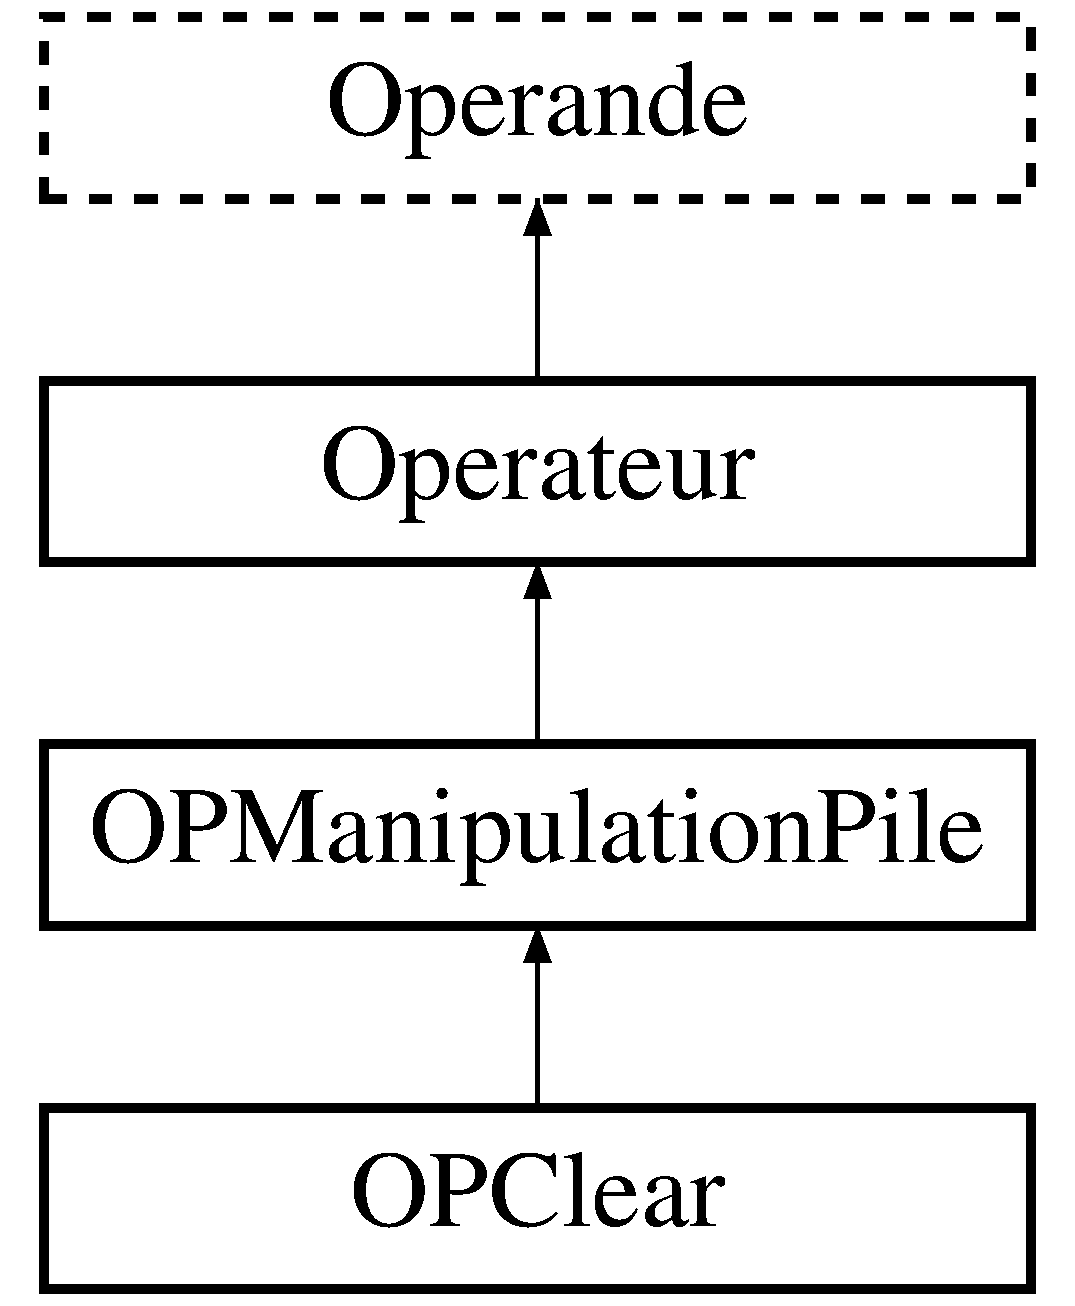
\includegraphics[height=4.000000cm]{class_o_p_clear}
\end{center}
\end{figure}
\subsection*{Public Member Functions}
\begin{DoxyCompactItemize}
\item 
virtual \hyperlink{class_o_p_clear}{O\+P\+Clear} $\ast$ {\bfseries clone} () const \hypertarget{class_o_p_clear_a32bdcfc46b4d04179154ae61d01b2448}{}\label{class_o_p_clear_a32bdcfc46b4d04179154ae61d01b2448}

\item 
virtual \hyperlink{class_litterale}{Litterale} $\ast$ {\bfseries compute} ()\hypertarget{class_o_p_clear_ad241fe8f1562ef42f2278416792c0865}{}\label{class_o_p_clear_ad241fe8f1562ef42f2278416792c0865}

\item 
virtual \hyperlink{class_litterale}{Litterale} $\ast$ {\bfseries compute} (\hyperlink{class_litterale}{Litterale} $\ast$l)\hypertarget{class_o_p_clear_ac84498a89811d3519d8b58ad3fc8e6e7}{}\label{class_o_p_clear_ac84498a89811d3519d8b58ad3fc8e6e7}

\item 
virtual \hyperlink{class_litterale}{Litterale} $\ast$ {\bfseries compute} (\hyperlink{class_litterale}{Litterale} $\ast$l1, \hyperlink{class_litterale}{Litterale} $\ast$l2)\hypertarget{class_o_p_clear_ac3e6e5fa309a868eac86b0e25481bc6c}{}\label{class_o_p_clear_ac3e6e5fa309a868eac86b0e25481bc6c}

\end{DoxyCompactItemize}
\subsection*{Additional Inherited Members}


The documentation for this class was generated from the following files\+:\begin{DoxyCompactItemize}
\item 
opmanipulationpile.\+h\item 
opmanipulationpile.\+cpp\end{DoxyCompactItemize}

\hypertarget{class_o_p_complexe}{}\section{O\+P\+Complexe Class Reference}
\label{class_o_p_complexe}\index{O\+P\+Complexe@{O\+P\+Complexe}}
Inheritance diagram for O\+P\+Complexe\+:\begin{figure}[H]
\begin{center}
\leavevmode
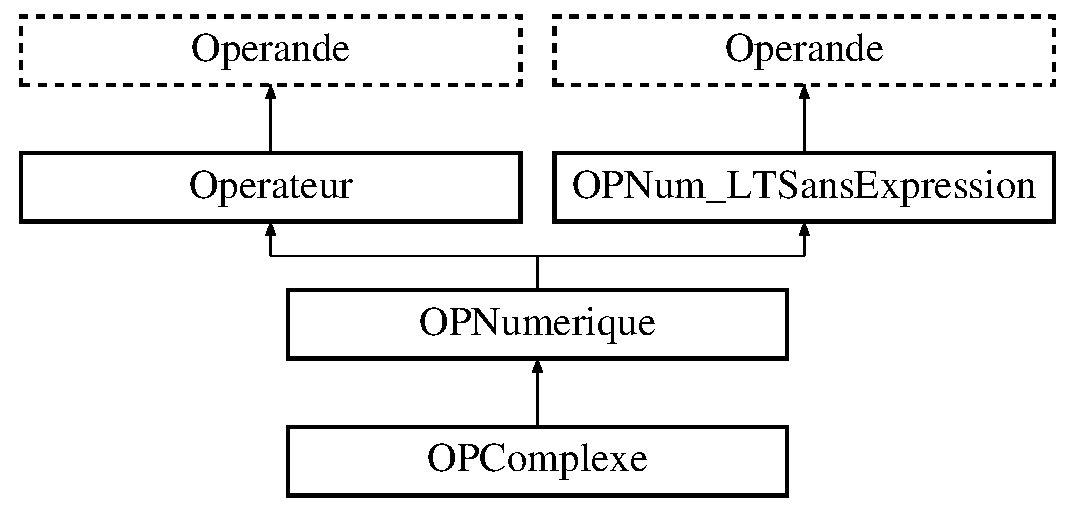
\includegraphics[height=4.000000cm]{class_o_p_complexe}
\end{center}
\end{figure}
\subsection*{Public Member Functions}
\begin{DoxyCompactItemize}
\item 
virtual \hyperlink{class_o_p_complexe}{O\+P\+Complexe} $\ast$ {\bfseries clone} () const \hypertarget{class_o_p_complexe_a33aab0fa1c6518a7c2db95a5eeded964}{}\label{class_o_p_complexe_a33aab0fa1c6518a7c2db95a5eeded964}

\item 
virtual \hyperlink{class_litterale}{Litterale} $\ast$ {\bfseries compute} ()\hypertarget{class_o_p_complexe_a0579bc96abf0c5eb42949b43c411236a}{}\label{class_o_p_complexe_a0579bc96abf0c5eb42949b43c411236a}

\item 
virtual \hyperlink{class_litterale}{Litterale} $\ast$ {\bfseries compute} (\hyperlink{class_litterale}{Litterale} $\ast$l)\hypertarget{class_o_p_complexe_a14b956eb146bfa0af0bd34238735b67f}{}\label{class_o_p_complexe_a14b956eb146bfa0af0bd34238735b67f}

\item 
virtual \hyperlink{class_litterale}{Litterale} $\ast$ {\bfseries compute} (\hyperlink{class_litterale}{Litterale} $\ast$l1, \hyperlink{class_litterale}{Litterale} $\ast$l2)\hypertarget{class_o_p_complexe_a38de10b8a869b84865cb06b84ead7364}{}\label{class_o_p_complexe_a38de10b8a869b84865cb06b84ead7364}

\end{DoxyCompactItemize}
\subsection*{Additional Inherited Members}


The documentation for this class was generated from the following files\+:\begin{DoxyCompactItemize}
\item 
opnumerique.\+h\item 
opnumerique.\+cpp\end{DoxyCompactItemize}

\hypertarget{class_o_p_conditionnel_boucle}{}\section{O\+P\+Conditionnel\+Boucle Class Reference}
\label{class_o_p_conditionnel_boucle}\index{O\+P\+Conditionnel\+Boucle@{O\+P\+Conditionnel\+Boucle}}
Inheritance diagram for O\+P\+Conditionnel\+Boucle\+:\begin{figure}[H]
\begin{center}
\leavevmode
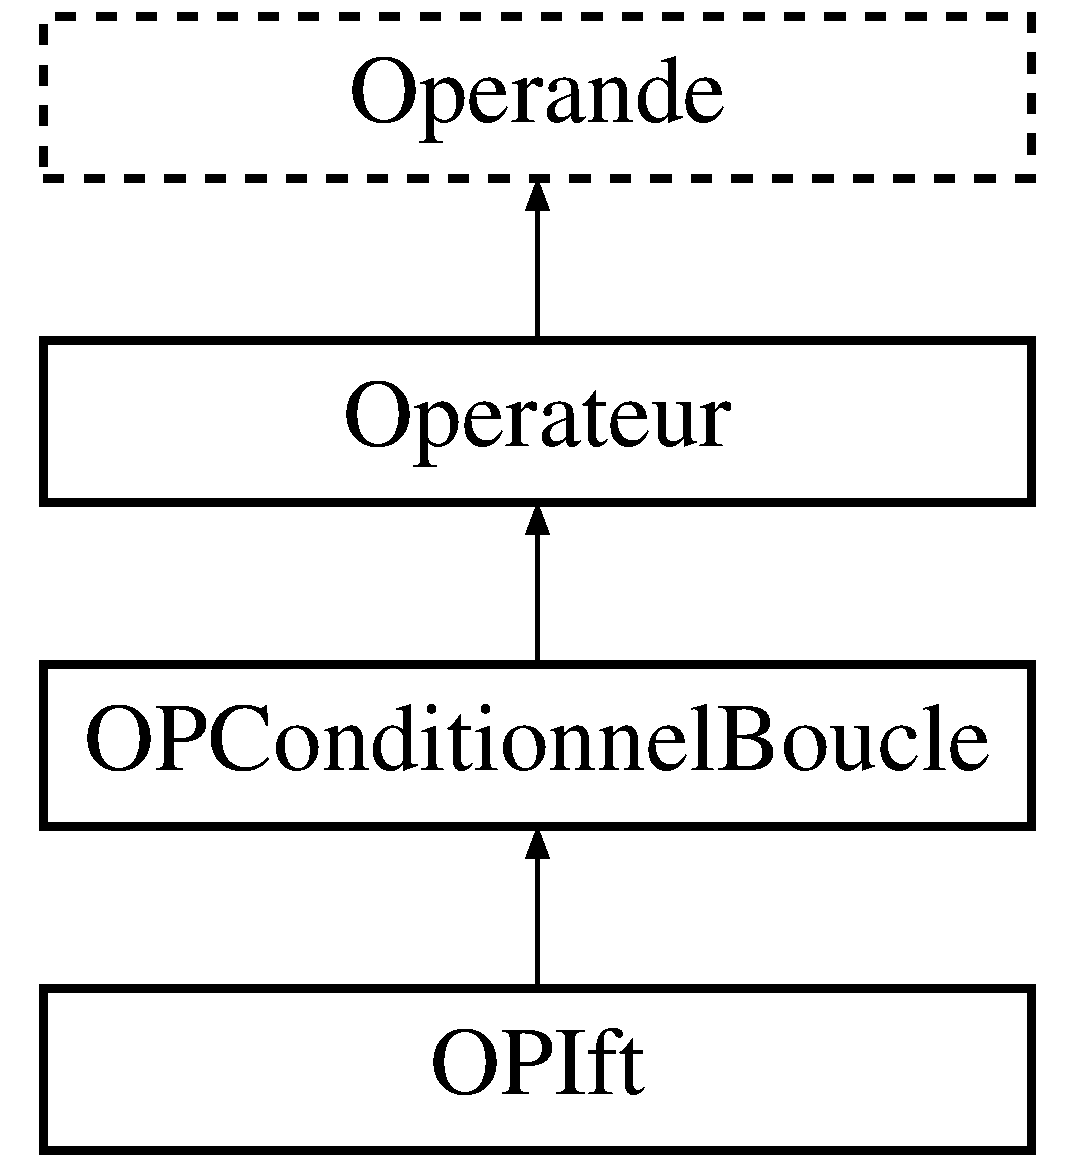
\includegraphics[height=4.000000cm]{class_o_p_conditionnel_boucle}
\end{center}
\end{figure}
\subsection*{Public Member Functions}
\begin{DoxyCompactItemize}
\item 
{\bfseries O\+P\+Conditionnel\+Boucle} (Q\+String val, int a)\hypertarget{class_o_p_conditionnel_boucle_aa69b34551b9448eab78a963d83c49df2}{}\label{class_o_p_conditionnel_boucle_aa69b34551b9448eab78a963d83c49df2}

\item 
virtual \hyperlink{class_o_p_conditionnel_boucle}{O\+P\+Conditionnel\+Boucle} $\ast$ {\bfseries clone} () const  =0\hypertarget{class_o_p_conditionnel_boucle_a1226ae17a78455d33c39f95e237ba9fe}{}\label{class_o_p_conditionnel_boucle_a1226ae17a78455d33c39f95e237ba9fe}

\item 
virtual \hyperlink{class_litterale}{Litterale} $\ast$ {\bfseries compute} ()=0\hypertarget{class_o_p_conditionnel_boucle_accae5fd1c376bbe40b52cbedfada5520}{}\label{class_o_p_conditionnel_boucle_accae5fd1c376bbe40b52cbedfada5520}

\item 
virtual \hyperlink{class_litterale}{Litterale} $\ast$ {\bfseries compute} (\hyperlink{class_litterale}{Litterale} $\ast$l)=0\hypertarget{class_o_p_conditionnel_boucle_a75c635c5356c47c0febdb85eef26e4da}{}\label{class_o_p_conditionnel_boucle_a75c635c5356c47c0febdb85eef26e4da}

\item 
virtual \hyperlink{class_litterale}{Litterale} $\ast$ {\bfseries compute} (\hyperlink{class_litterale}{Litterale} $\ast$l1, \hyperlink{class_litterale}{Litterale} $\ast$l2)=0\hypertarget{class_o_p_conditionnel_boucle_a3eb3f1c30233f5ced899ad44ad85374c}{}\label{class_o_p_conditionnel_boucle_a3eb3f1c30233f5ced899ad44ad85374c}

\end{DoxyCompactItemize}
\subsection*{Additional Inherited Members}


The documentation for this class was generated from the following file\+:\begin{DoxyCompactItemize}
\item 
opconditionnelboucle.\+h\end{DoxyCompactItemize}

\hypertarget{class_o_p_denominateur}{}\section{O\+P\+Denominateur Class Reference}
\label{class_o_p_denominateur}\index{O\+P\+Denominateur@{O\+P\+Denominateur}}
Inheritance diagram for O\+P\+Denominateur\+:\begin{figure}[H]
\begin{center}
\leavevmode
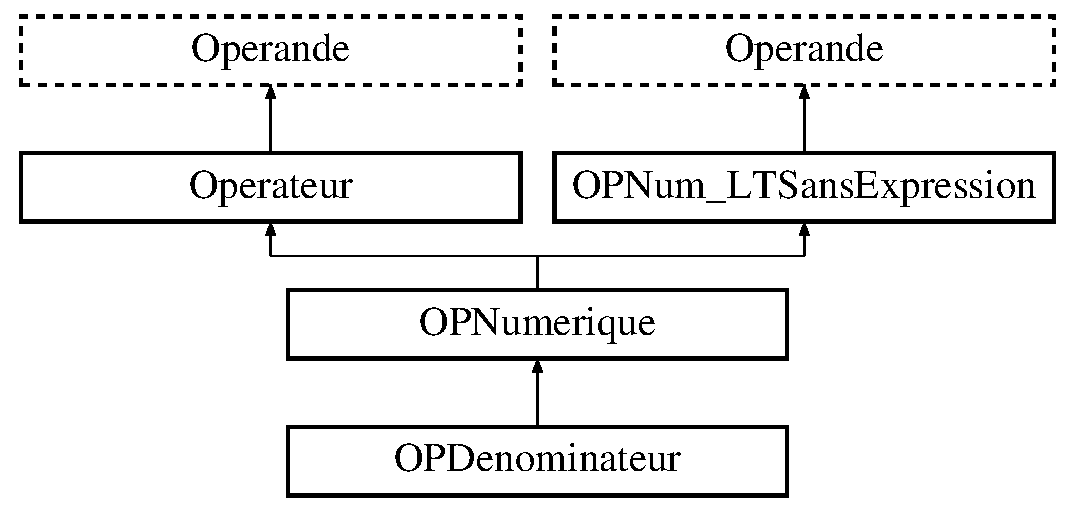
\includegraphics[height=4.000000cm]{class_o_p_denominateur}
\end{center}
\end{figure}
\subsection*{Public Member Functions}
\begin{DoxyCompactItemize}
\item 
virtual \hyperlink{class_o_p_denominateur}{O\+P\+Denominateur} $\ast$ {\bfseries clone} () const \hypertarget{class_o_p_denominateur_a325d837c2c74e246a53615b087130765}{}\label{class_o_p_denominateur_a325d837c2c74e246a53615b087130765}

\item 
virtual \hyperlink{class_litterale}{Litterale} $\ast$ {\bfseries compute} ()\hypertarget{class_o_p_denominateur_a982e8e23e558352486d172d852aa732d}{}\label{class_o_p_denominateur_a982e8e23e558352486d172d852aa732d}

\item 
virtual \hyperlink{class_litterale}{Litterale} $\ast$ {\bfseries compute} (\hyperlink{class_litterale}{Litterale} $\ast$l)\hypertarget{class_o_p_denominateur_af95c5033dd9770a3ec23b72d73fa9e24}{}\label{class_o_p_denominateur_af95c5033dd9770a3ec23b72d73fa9e24}

\item 
virtual \hyperlink{class_litterale}{Litterale} $\ast$ {\bfseries compute} (\hyperlink{class_litterale}{Litterale} $\ast$l1, \hyperlink{class_litterale}{Litterale} $\ast$l2)\hypertarget{class_o_p_denominateur_ad099dbca81442d91c6721c89a7a36a7b}{}\label{class_o_p_denominateur_ad099dbca81442d91c6721c89a7a36a7b}

\end{DoxyCompactItemize}
\subsection*{Additional Inherited Members}


The documentation for this class was generated from the following files\+:\begin{DoxyCompactItemize}
\item 
opnumerique.\+h\item 
opnumerique.\+cpp\end{DoxyCompactItemize}

\hypertarget{class_o_p_different}{}\section{O\+P\+Different Class Reference}
\label{class_o_p_different}\index{O\+P\+Different@{O\+P\+Different}}
Inheritance diagram for O\+P\+Different\+:\begin{figure}[H]
\begin{center}
\leavevmode
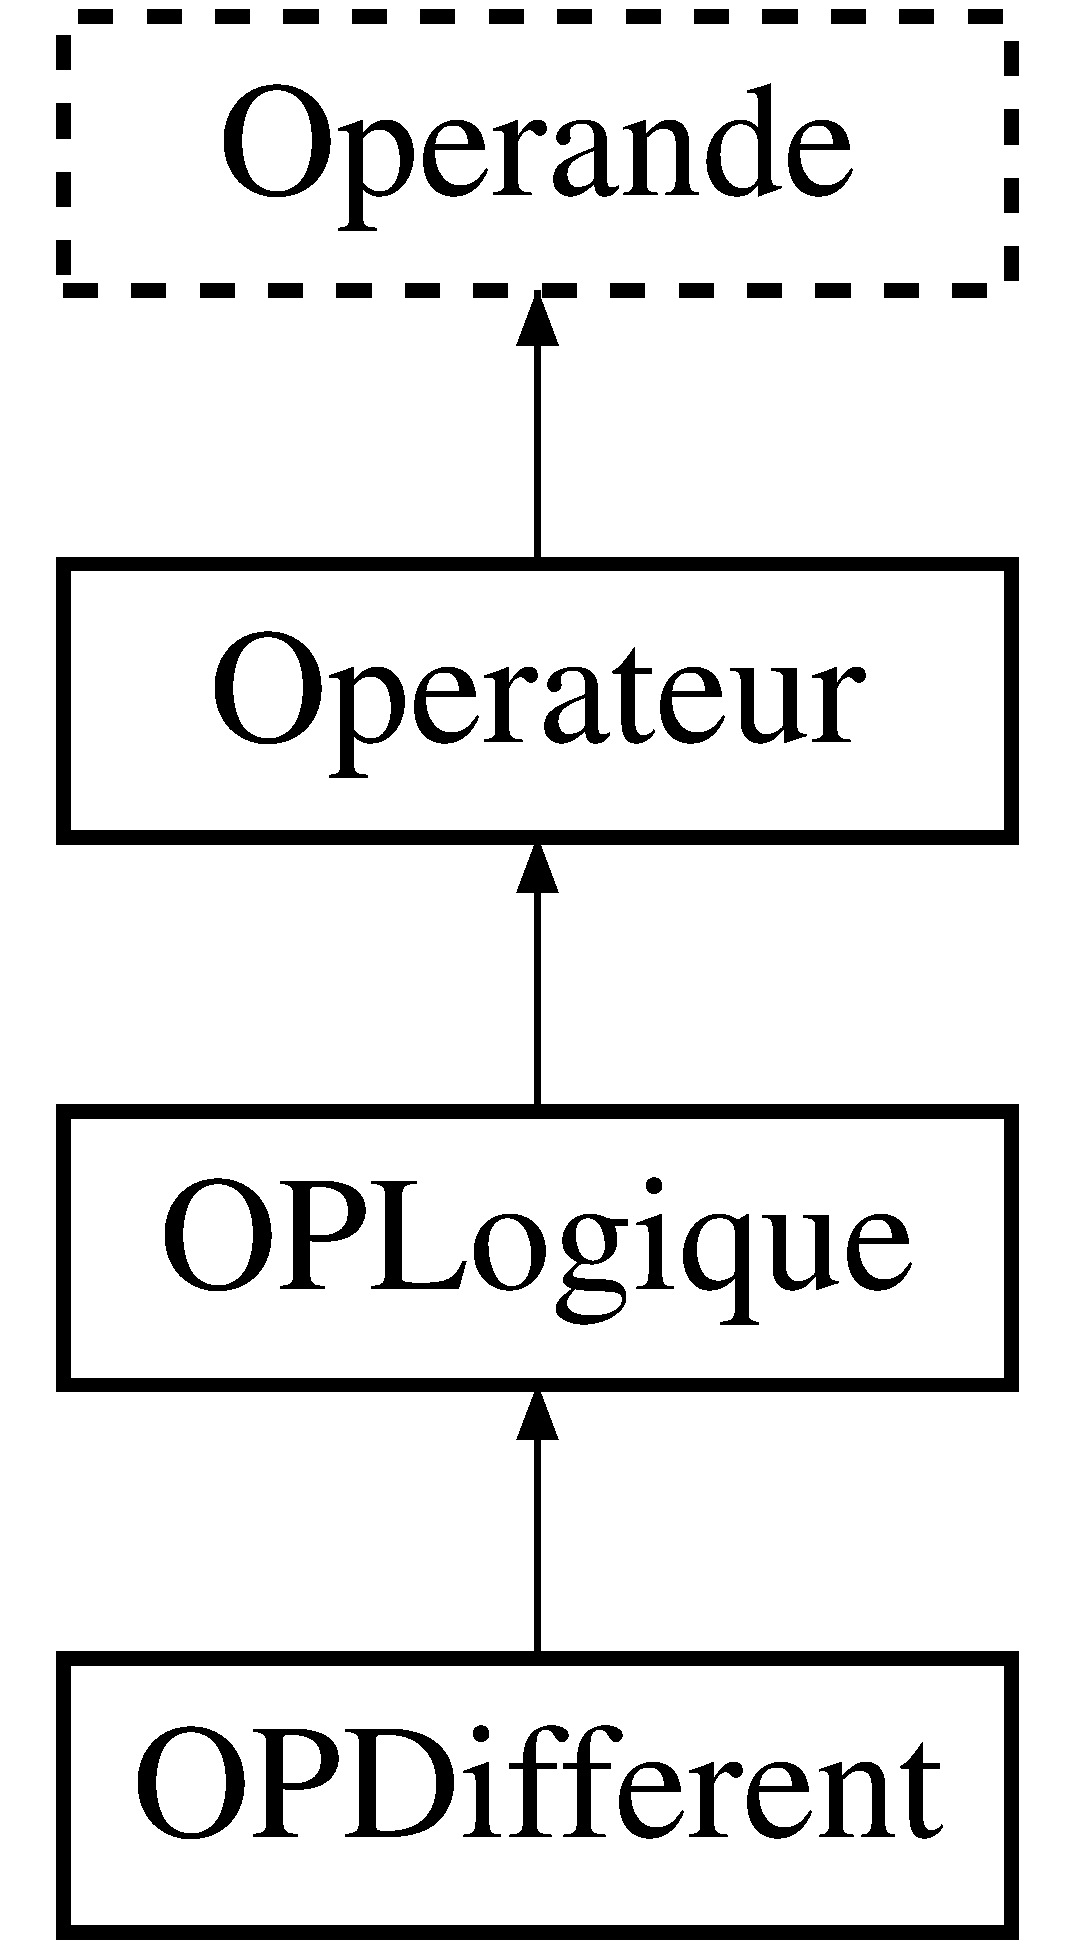
\includegraphics[height=4.000000cm]{class_o_p_different}
\end{center}
\end{figure}
\subsection*{Public Member Functions}
\begin{DoxyCompactItemize}
\item 
virtual \hyperlink{class_o_p_different}{O\+P\+Different} $\ast$ {\bfseries clone} () const \hypertarget{class_o_p_different_a5ce33f9701f513327da5d2b4ae6a5567}{}\label{class_o_p_different_a5ce33f9701f513327da5d2b4ae6a5567}

\item 
virtual \hyperlink{class_litterale}{Litterale} $\ast$ {\bfseries compute} ()\hypertarget{class_o_p_different_a6ad8f42f202de22de29a39325b3ea884}{}\label{class_o_p_different_a6ad8f42f202de22de29a39325b3ea884}

\item 
virtual \hyperlink{class_litterale}{Litterale} $\ast$ {\bfseries compute} (\hyperlink{class_litterale}{Litterale} $\ast$l)\hypertarget{class_o_p_different_aeba793fc46067933df8f1d9374ba0b56}{}\label{class_o_p_different_aeba793fc46067933df8f1d9374ba0b56}

\item 
virtual \hyperlink{class_litterale}{Litterale} $\ast$ {\bfseries compute} (\hyperlink{class_litterale}{Litterale} $\ast$l1, \hyperlink{class_litterale}{Litterale} $\ast$l2)\hypertarget{class_o_p_different_a0558fae2b6cd09f4ada9b13be4f8c6e4}{}\label{class_o_p_different_a0558fae2b6cd09f4ada9b13be4f8c6e4}

\end{DoxyCompactItemize}
\subsection*{Additional Inherited Members}


The documentation for this class was generated from the following files\+:\begin{DoxyCompactItemize}
\item 
oplogique.\+h\item 
oplogique.\+cpp\end{DoxyCompactItemize}

\hypertarget{class_o_p_division}{}\section{O\+P\+Division Class Reference}
\label{class_o_p_division}\index{O\+P\+Division@{O\+P\+Division}}
Inheritance diagram for O\+P\+Division\+:\begin{figure}[H]
\begin{center}
\leavevmode
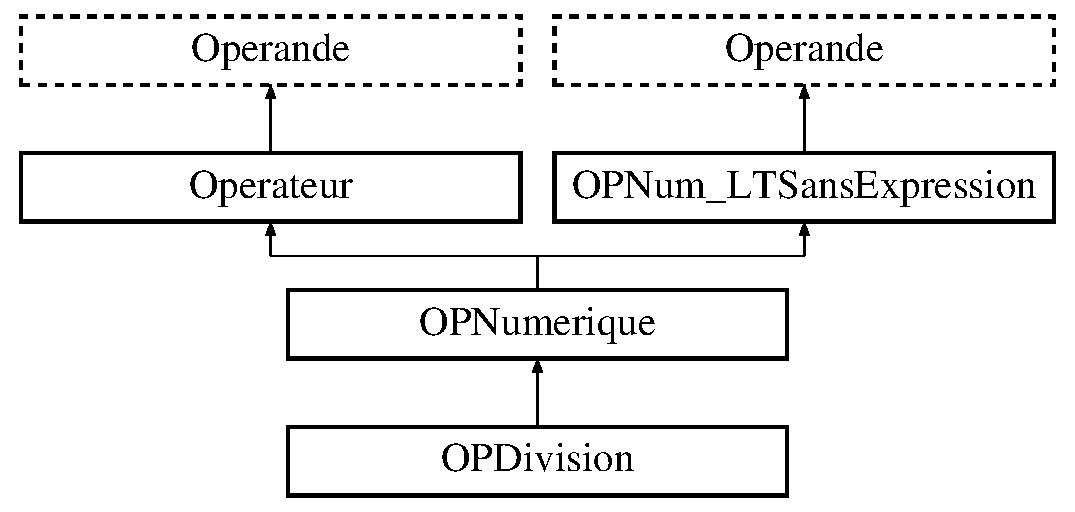
\includegraphics[height=4.000000cm]{class_o_p_division}
\end{center}
\end{figure}
\subsection*{Public Member Functions}
\begin{DoxyCompactItemize}
\item 
virtual \hyperlink{class_o_p_division}{O\+P\+Division} $\ast$ {\bfseries clone} () const \hypertarget{class_o_p_division_a44f273e86a016e7cc740940a93dfe6bb}{}\label{class_o_p_division_a44f273e86a016e7cc740940a93dfe6bb}

\item 
virtual \hyperlink{class_litterale}{Litterale} $\ast$ {\bfseries compute} ()\hypertarget{class_o_p_division_ab1fd1dd980e13a2f6e2f8d4992e20a21}{}\label{class_o_p_division_ab1fd1dd980e13a2f6e2f8d4992e20a21}

\item 
virtual \hyperlink{class_litterale}{Litterale} $\ast$ {\bfseries compute} (\hyperlink{class_litterale}{Litterale} $\ast$l)\hypertarget{class_o_p_division_a2e46542094502a4b8d8743d82ad1d678}{}\label{class_o_p_division_a2e46542094502a4b8d8743d82ad1d678}

\item 
virtual \hyperlink{class_litterale}{Litterale} $\ast$ {\bfseries compute} (\hyperlink{class_litterale}{Litterale} $\ast$l1, \hyperlink{class_litterale}{Litterale} $\ast$l2)\hypertarget{class_o_p_division_a5903fe056c0541a188c2ce9fd6a510c5}{}\label{class_o_p_division_a5903fe056c0541a188c2ce9fd6a510c5}

\end{DoxyCompactItemize}
\subsection*{Additional Inherited Members}


The documentation for this class was generated from the following files\+:\begin{DoxyCompactItemize}
\item 
opnumerique.\+h\item 
opnumerique.\+cpp\end{DoxyCompactItemize}

\hypertarget{class_o_p_division_entiere}{}\section{O\+P\+Division\+Entiere Class Reference}
\label{class_o_p_division_entiere}\index{O\+P\+Division\+Entiere@{O\+P\+Division\+Entiere}}
Inheritance diagram for O\+P\+Division\+Entiere\+:\begin{figure}[H]
\begin{center}
\leavevmode
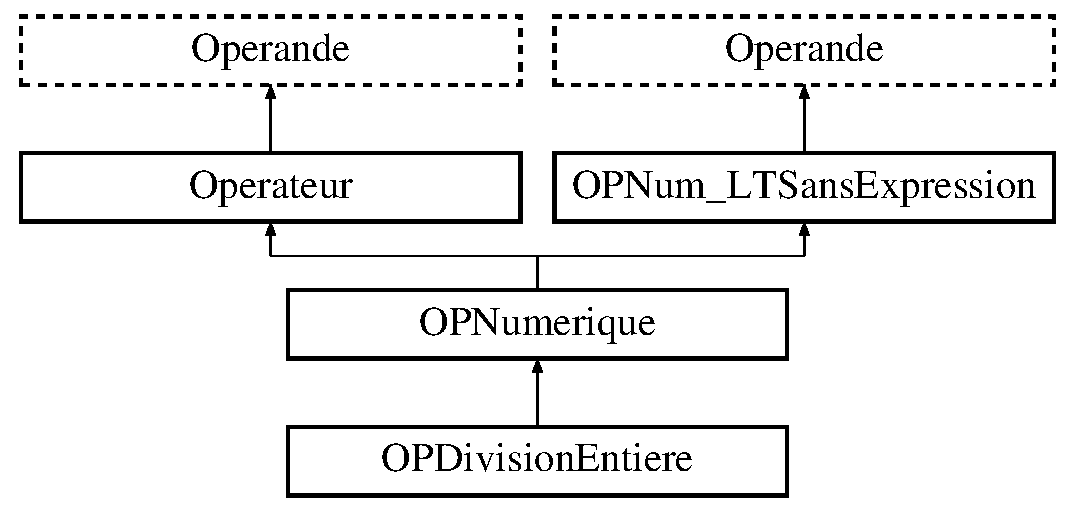
\includegraphics[height=4.000000cm]{class_o_p_division_entiere}
\end{center}
\end{figure}
\subsection*{Public Member Functions}
\begin{DoxyCompactItemize}
\item 
virtual \hyperlink{class_o_p_division_entiere}{O\+P\+Division\+Entiere} $\ast$ {\bfseries clone} () const \hypertarget{class_o_p_division_entiere_ae90f3aa4aca15926450391a380de0951}{}\label{class_o_p_division_entiere_ae90f3aa4aca15926450391a380de0951}

\item 
virtual \hyperlink{class_litterale}{Litterale} $\ast$ {\bfseries compute} ()\hypertarget{class_o_p_division_entiere_aeb20c22302666079c2c56eea544a04ce}{}\label{class_o_p_division_entiere_aeb20c22302666079c2c56eea544a04ce}

\item 
virtual \hyperlink{class_litterale}{Litterale} $\ast$ {\bfseries compute} (\hyperlink{class_litterale}{Litterale} $\ast$l)\hypertarget{class_o_p_division_entiere_a23786ead1ed63789b3b94025a1496fb0}{}\label{class_o_p_division_entiere_a23786ead1ed63789b3b94025a1496fb0}

\item 
virtual \hyperlink{class_litterale}{Litterale} $\ast$ {\bfseries compute} (\hyperlink{class_litterale}{Litterale} $\ast$l1, \hyperlink{class_litterale}{Litterale} $\ast$l2)\hypertarget{class_o_p_division_entiere_ad35d7790fe441a7ee109037d4f34d138}{}\label{class_o_p_division_entiere_ad35d7790fe441a7ee109037d4f34d138}

\end{DoxyCompactItemize}
\subsection*{Additional Inherited Members}


The documentation for this class was generated from the following files\+:\begin{DoxyCompactItemize}
\item 
opnumerique.\+h\item 
opnumerique.\+cpp\end{DoxyCompactItemize}

\hypertarget{class_o_p_drop}{}\section{O\+P\+Drop Class Reference}
\label{class_o_p_drop}\index{O\+P\+Drop@{O\+P\+Drop}}
Inheritance diagram for O\+P\+Drop\+:\begin{figure}[H]
\begin{center}
\leavevmode
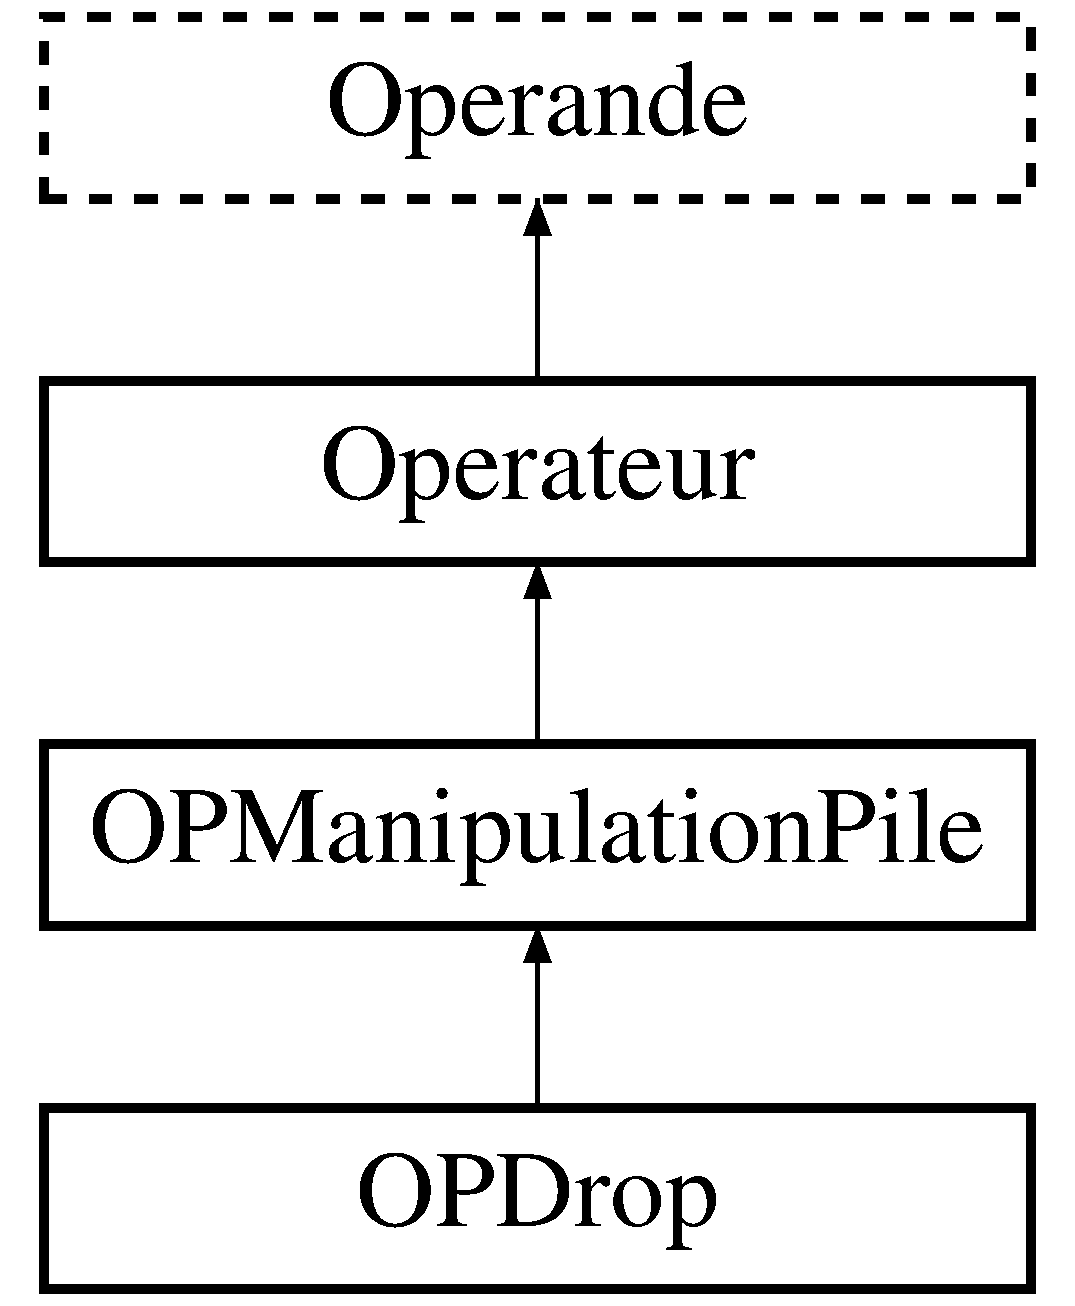
\includegraphics[height=4.000000cm]{class_o_p_drop}
\end{center}
\end{figure}
\subsection*{Public Member Functions}
\begin{DoxyCompactItemize}
\item 
virtual \hyperlink{class_o_p_drop}{O\+P\+Drop} $\ast$ {\bfseries clone} () const \hypertarget{class_o_p_drop_a9023aab083de2456f6155bebeadbd9a7}{}\label{class_o_p_drop_a9023aab083de2456f6155bebeadbd9a7}

\item 
virtual \hyperlink{class_litterale}{Litterale} $\ast$ {\bfseries compute} ()\hypertarget{class_o_p_drop_a3f8df81126b25afda7e3fd98274e0a7a}{}\label{class_o_p_drop_a3f8df81126b25afda7e3fd98274e0a7a}

\item 
virtual \hyperlink{class_litterale}{Litterale} $\ast$ {\bfseries compute} (\hyperlink{class_litterale}{Litterale} $\ast$l)\hypertarget{class_o_p_drop_a95e2bc8070e5430ba7e94d3bb0f490d0}{}\label{class_o_p_drop_a95e2bc8070e5430ba7e94d3bb0f490d0}

\item 
virtual \hyperlink{class_litterale}{Litterale} $\ast$ {\bfseries compute} (\hyperlink{class_litterale}{Litterale} $\ast$l1, \hyperlink{class_litterale}{Litterale} $\ast$l2)\hypertarget{class_o_p_drop_a806a7c17d9a7bc8e5c4cba6314e65686}{}\label{class_o_p_drop_a806a7c17d9a7bc8e5c4cba6314e65686}

\end{DoxyCompactItemize}
\subsection*{Additional Inherited Members}


The documentation for this class was generated from the following files\+:\begin{DoxyCompactItemize}
\item 
opmanipulationpile.\+h\item 
opmanipulationpile.\+cpp\end{DoxyCompactItemize}

\hypertarget{class_o_p_dup}{}\section{O\+P\+Dup Class Reference}
\label{class_o_p_dup}\index{O\+P\+Dup@{O\+P\+Dup}}
Inheritance diagram for O\+P\+Dup\+:\begin{figure}[H]
\begin{center}
\leavevmode
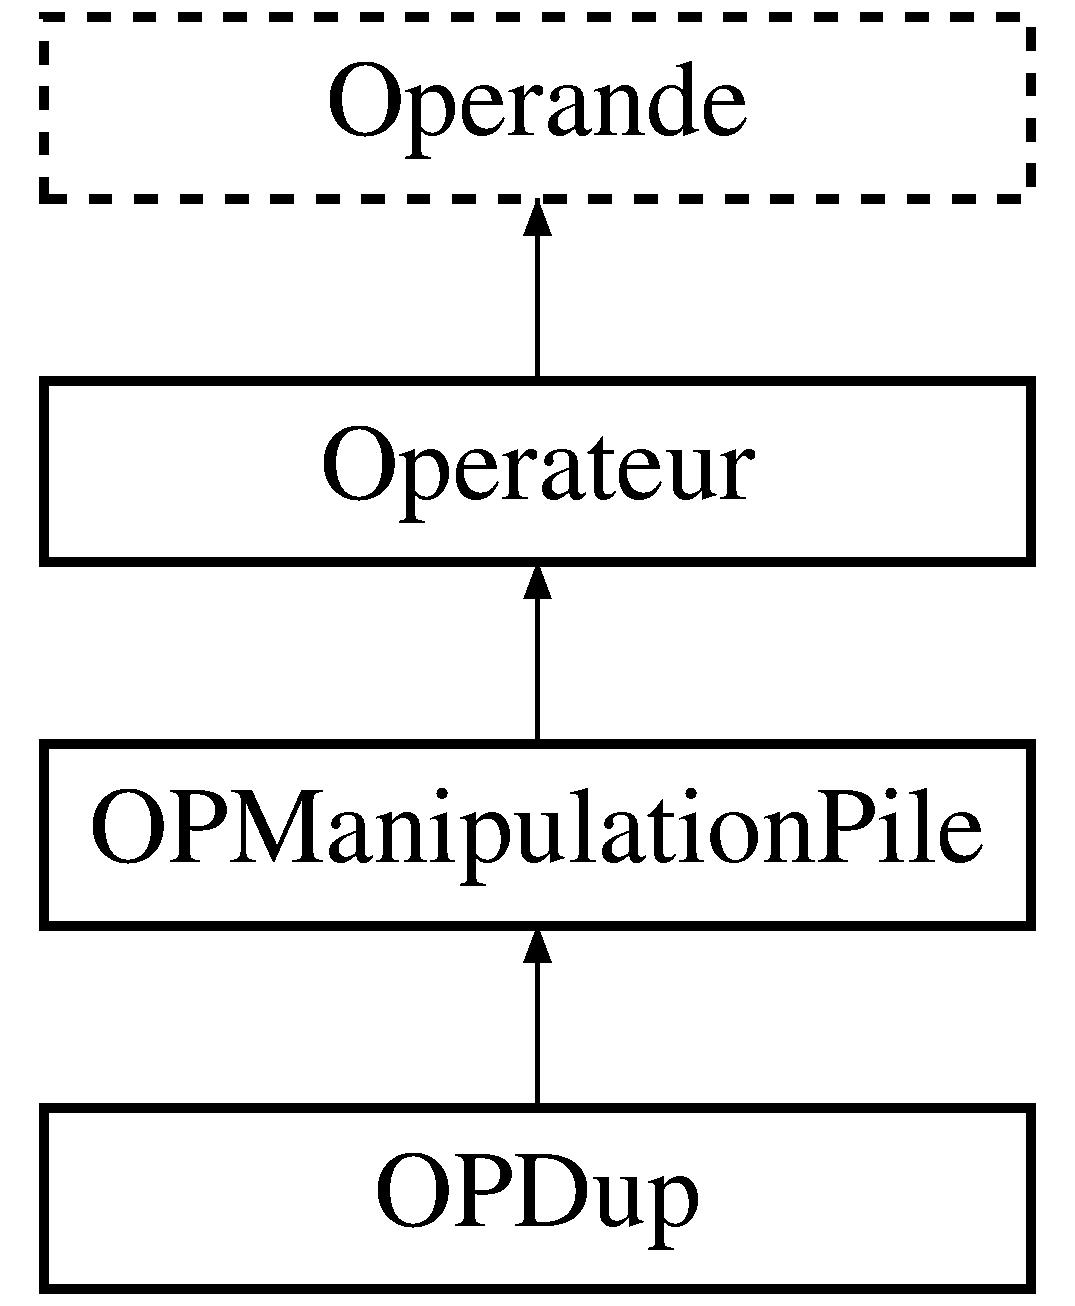
\includegraphics[height=4.000000cm]{class_o_p_dup}
\end{center}
\end{figure}
\subsection*{Public Member Functions}
\begin{DoxyCompactItemize}
\item 
virtual \hyperlink{class_o_p_dup}{O\+P\+Dup} $\ast$ {\bfseries clone} () const \hypertarget{class_o_p_dup_a193c5d1707956c45d83dd1f90338a412}{}\label{class_o_p_dup_a193c5d1707956c45d83dd1f90338a412}

\item 
virtual \hyperlink{class_litterale}{Litterale} $\ast$ {\bfseries compute} ()\hypertarget{class_o_p_dup_a155c182db91aed7d472cfb624fa01a99}{}\label{class_o_p_dup_a155c182db91aed7d472cfb624fa01a99}

\item 
virtual \hyperlink{class_litterale}{Litterale} $\ast$ {\bfseries compute} (\hyperlink{class_litterale}{Litterale} $\ast$l)\hypertarget{class_o_p_dup_a555ea493eee87bb8b9b4d2c66c9210b8}{}\label{class_o_p_dup_a555ea493eee87bb8b9b4d2c66c9210b8}

\item 
virtual \hyperlink{class_litterale}{Litterale} $\ast$ {\bfseries compute} (\hyperlink{class_litterale}{Litterale} $\ast$l1, \hyperlink{class_litterale}{Litterale} $\ast$l2)\hypertarget{class_o_p_dup_af761a9cb8f7d5c8e16681b46f9e03192}{}\label{class_o_p_dup_af761a9cb8f7d5c8e16681b46f9e03192}

\end{DoxyCompactItemize}
\subsection*{Additional Inherited Members}


The documentation for this class was generated from the following files\+:\begin{DoxyCompactItemize}
\item 
opmanipulationpile.\+h\item 
opmanipulationpile.\+cpp\end{DoxyCompactItemize}

\hypertarget{class_o_p_edit}{}\section{O\+P\+Edit Class Reference}
\label{class_o_p_edit}\index{O\+P\+Edit@{O\+P\+Edit}}
Inheritance diagram for O\+P\+Edit\+:\begin{figure}[H]
\begin{center}
\leavevmode
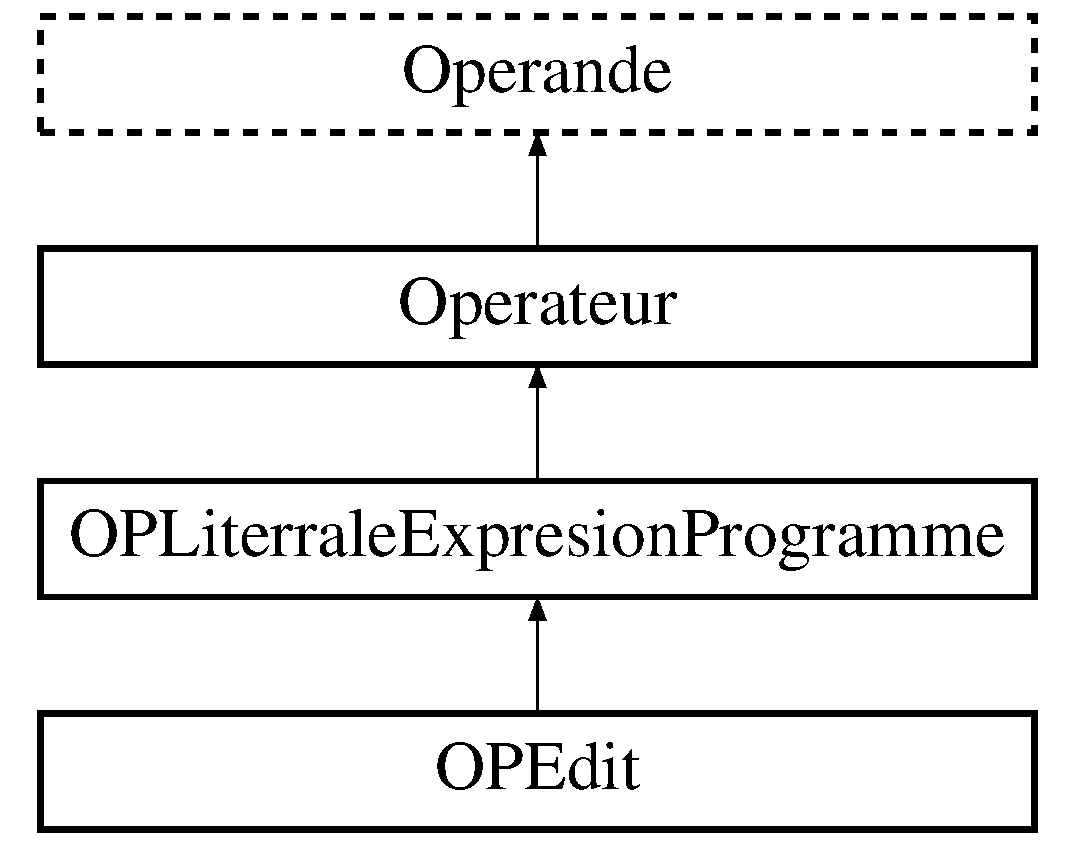
\includegraphics[height=4.000000cm]{class_o_p_edit}
\end{center}
\end{figure}
\subsection*{Public Member Functions}
\begin{DoxyCompactItemize}
\item 
virtual \hyperlink{class_o_p_edit}{O\+P\+Edit} $\ast$ {\bfseries clone} () const \hypertarget{class_o_p_edit_ab70b709ea9b4281651583632e0e84456}{}\label{class_o_p_edit_ab70b709ea9b4281651583632e0e84456}

\item 
virtual \hyperlink{class_litterale}{Litterale} $\ast$ {\bfseries compute} ()\hypertarget{class_o_p_edit_a9eb95efcb93c180eb1436d327be5c136}{}\label{class_o_p_edit_a9eb95efcb93c180eb1436d327be5c136}

\item 
virtual \hyperlink{class_litterale}{Litterale} $\ast$ {\bfseries compute} (\hyperlink{class_litterale}{Litterale} $\ast$l)\hypertarget{class_o_p_edit_a21615280952f453fcf586711591f6e97}{}\label{class_o_p_edit_a21615280952f453fcf586711591f6e97}

\item 
virtual \hyperlink{class_litterale}{Litterale} $\ast$ {\bfseries compute} (\hyperlink{class_litterale}{Litterale} $\ast$l1, \hyperlink{class_litterale}{Litterale} $\ast$l2)\hypertarget{class_o_p_edit_aaa16d6e4a144f1a881eb61770ca6ec03}{}\label{class_o_p_edit_aaa16d6e4a144f1a881eb61770ca6ec03}

\end{DoxyCompactItemize}
\subsection*{Additional Inherited Members}


The documentation for this class was generated from the following files\+:\begin{DoxyCompactItemize}
\item 
opliterraleexpresionprogramme.\+h\item 
opliterraleexpresionprogramme.\+cpp\end{DoxyCompactItemize}

\hypertarget{class_o_p_egal}{}\section{O\+P\+Egal Class Reference}
\label{class_o_p_egal}\index{O\+P\+Egal@{O\+P\+Egal}}
Inheritance diagram for O\+P\+Egal\+:\begin{figure}[H]
\begin{center}
\leavevmode
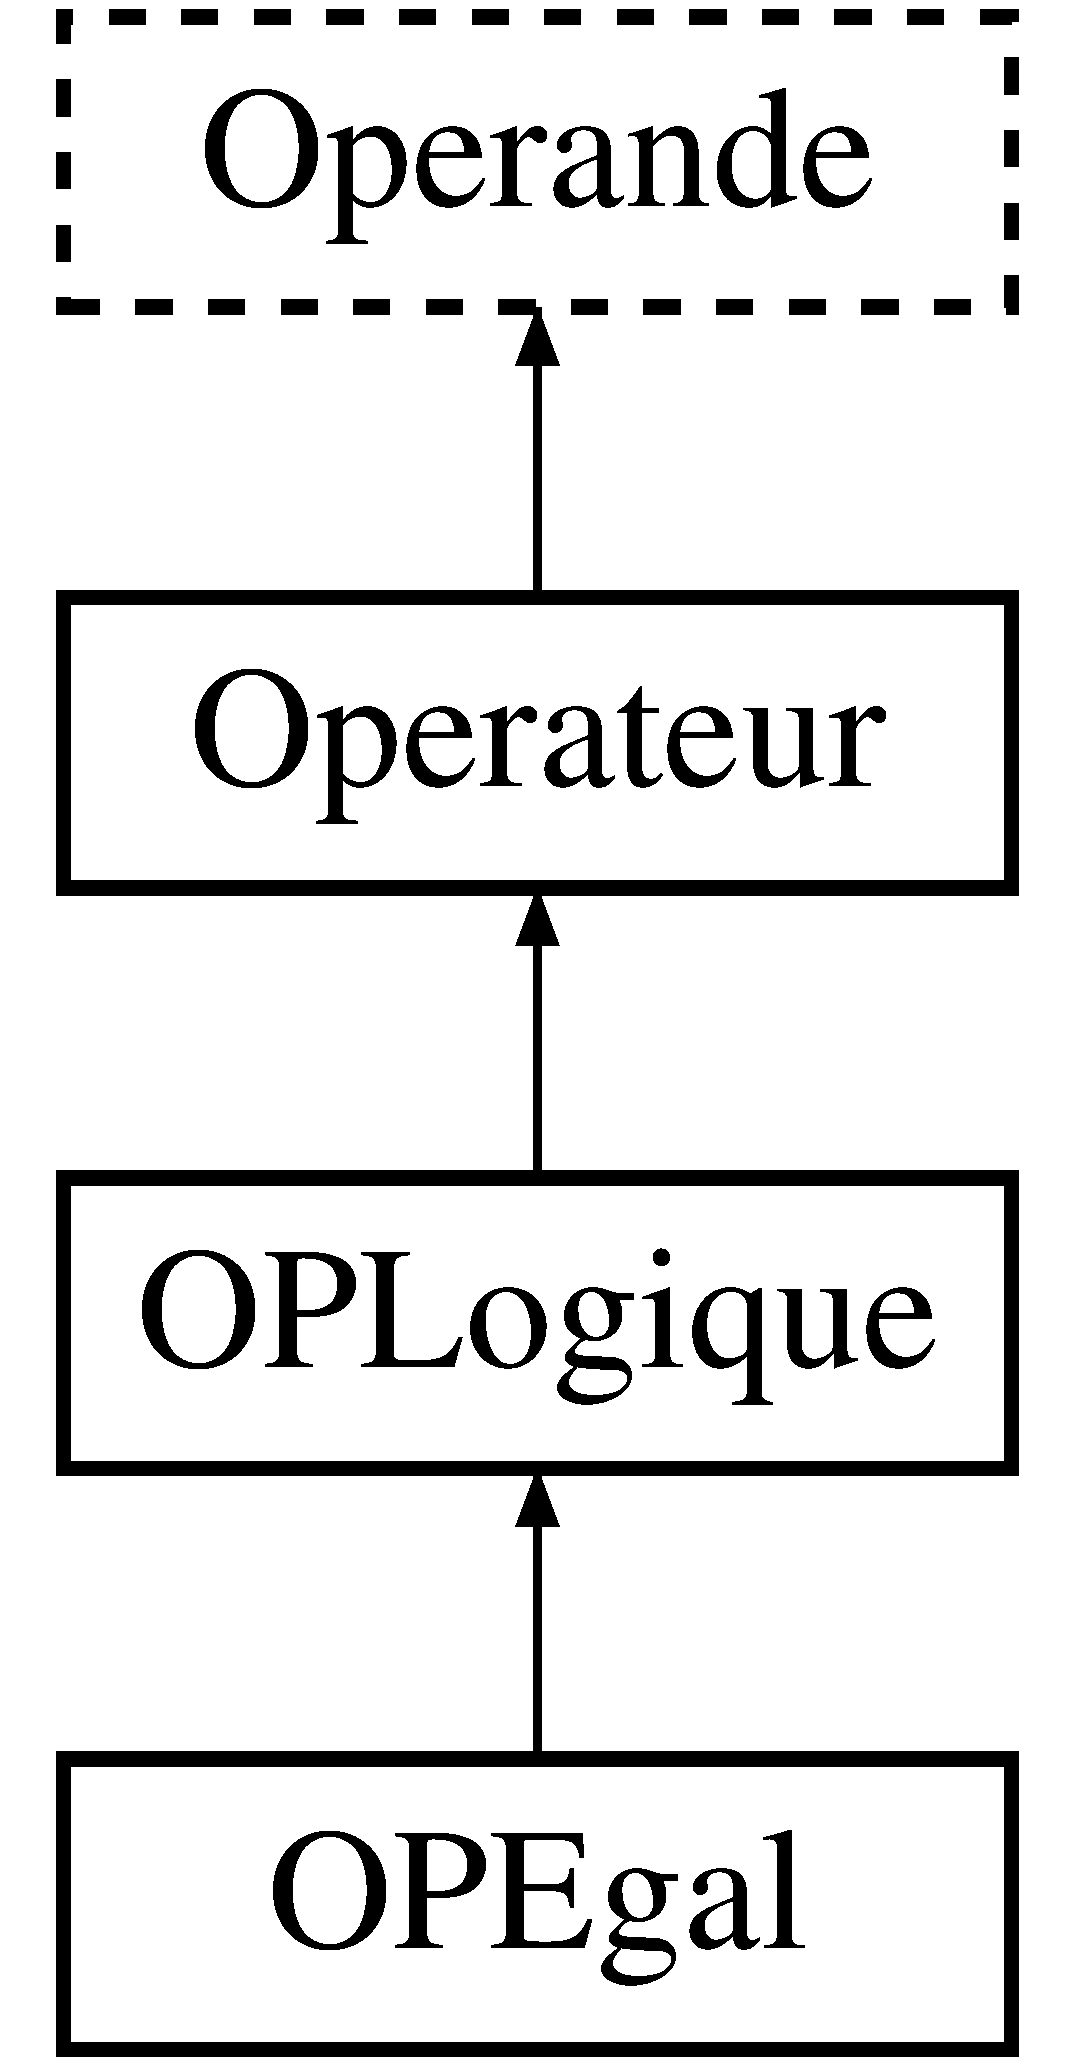
\includegraphics[height=4.000000cm]{class_o_p_egal}
\end{center}
\end{figure}
\subsection*{Public Member Functions}
\begin{DoxyCompactItemize}
\item 
virtual \hyperlink{class_o_p_egal}{O\+P\+Egal} $\ast$ {\bfseries clone} () const \hypertarget{class_o_p_egal_a7e09ed34162cb2e56f6c6ee73662f564}{}\label{class_o_p_egal_a7e09ed34162cb2e56f6c6ee73662f564}

\item 
virtual \hyperlink{class_litterale}{Litterale} $\ast$ {\bfseries compute} ()\hypertarget{class_o_p_egal_a3303a6679e8353ef6517ca83344844f5}{}\label{class_o_p_egal_a3303a6679e8353ef6517ca83344844f5}

\item 
virtual \hyperlink{class_litterale}{Litterale} $\ast$ {\bfseries compute} (\hyperlink{class_litterale}{Litterale} $\ast$l)\hypertarget{class_o_p_egal_a2848159c99bef604362fbb580bb68e74}{}\label{class_o_p_egal_a2848159c99bef604362fbb580bb68e74}

\item 
virtual \hyperlink{class_litterale}{Litterale} $\ast$ {\bfseries compute} (\hyperlink{class_litterale}{Litterale} $\ast$l1, \hyperlink{class_litterale}{Litterale} $\ast$l2)\hypertarget{class_o_p_egal_adaf447809f230354de29788507db5dba}{}\label{class_o_p_egal_adaf447809f230354de29788507db5dba}

\end{DoxyCompactItemize}
\subsection*{Additional Inherited Members}


The documentation for this class was generated from the following files\+:\begin{DoxyCompactItemize}
\item 
oplogique.\+h\item 
oplogique.\+cpp\end{DoxyCompactItemize}

\hypertarget{class_operande}{}\section{Operande Class Reference}
\label{class_operande}\index{Operande@{Operande}}
Inheritance diagram for Operande\+:\begin{figure}[H]
\begin{center}
\leavevmode
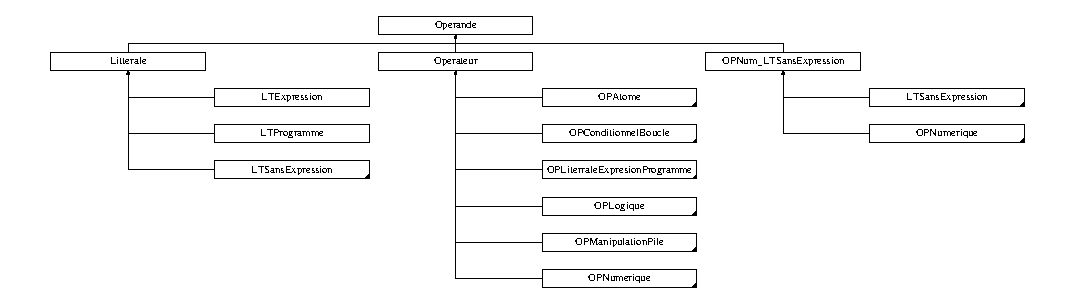
\includegraphics[height=3.642277cm]{class_operande}
\end{center}
\end{figure}
\subsection*{Public Member Functions}
\begin{DoxyCompactItemize}
\item 
virtual void {\bfseries afficher} () const  =0\hypertarget{class_operande_ad723ef2e33ae865728804e228f4f5375}{}\label{class_operande_ad723ef2e33ae865728804e228f4f5375}

\item 
virtual Q\+String {\bfseries get\+Text} () const  =0\hypertarget{class_operande_a90c9dc4b24eb4e4206e53cff622f6f6d}{}\label{class_operande_a90c9dc4b24eb4e4206e53cff622f6f6d}

\item 
virtual \hyperlink{class_operande}{Operande} $\ast$ {\bfseries clone} () const  =0\hypertarget{class_operande_a9fccf1533e1f7bfcdbdaf0c448a013b9}{}\label{class_operande_a9fccf1533e1f7bfcdbdaf0c448a013b9}

\end{DoxyCompactItemize}


The documentation for this class was generated from the following file\+:\begin{DoxyCompactItemize}
\item 
operande.\+h\end{DoxyCompactItemize}

\hypertarget{class_operande_factory}{}\section{Operande\+Factory Class Reference}
\label{class_operande_factory}\index{Operande\+Factory@{Operande\+Factory}}
\subsection*{Static Public Member Functions}
\begin{DoxyCompactItemize}
\item 
static \hyperlink{class_operande}{Operande} $\ast$ {\bfseries New\+Operande} (const Q\+String \&str)\hypertarget{class_operande_factory_af20bfb7436b73504423a0b566c6aac5f}{}\label{class_operande_factory_af20bfb7436b73504423a0b566c6aac5f}

\item 
static \hyperlink{class_o_p_num___l_t_sans_expression}{O\+P\+Num\+\_\+\+L\+T\+Sans\+Expression} $\ast$ {\bfseries New\+O\+P\+Num\+\_\+\+L\+T\+Sans\+Expression} (const Q\+String \&str)\hypertarget{class_operande_factory_a6de4539897981c388493689aacacf548}{}\label{class_operande_factory_a6de4539897981c388493689aacacf548}

\item 
static bool {\bfseries is\+Operator} (Q\+String C)\hypertarget{class_operande_factory_ada8645a0a4971ebefcc9c24c761e46c4}{}\label{class_operande_factory_ada8645a0a4971ebefcc9c24c761e46c4}

\item 
static bool {\bfseries is\+Litterale} (const Q\+String \&symbol)\hypertarget{class_operande_factory_a547d3898588342c53951472b17ef9e53}{}\label{class_operande_factory_a547d3898588342c53951472b17ef9e53}

\item 
static int {\bfseries operator\+Weight} (Q\+String arg)\hypertarget{class_operande_factory_a6c3274fddb75b141d2c3ffa759f75358}{}\label{class_operande_factory_a6c3274fddb75b141d2c3ffa759f75358}

\item 
static int {\bfseries operateur\+Prioritaire} (Q\+String a, Q\+String b)\hypertarget{class_operande_factory_a7c418ffcba5c6a92e86784874a32b3e8}{}\label{class_operande_factory_a7c418ffcba5c6a92e86784874a32b3e8}

\item 
static Q\+String {\bfseries infix\+To\+Postfix} (Q\+String expr)\hypertarget{class_operande_factory_aff31ef33868512e10ff05189eb2468a4}{}\label{class_operande_factory_aff31ef33868512e10ff05189eb2468a4}

\item 
static Q\+String {\bfseries add\+Space} (Q\+String str)\hypertarget{class_operande_factory_a0dbc35bda53581379a2aa83f9c36b549}{}\label{class_operande_factory_a0dbc35bda53581379a2aa83f9c36b549}

\end{DoxyCompactItemize}


The documentation for this class was generated from the following files\+:\begin{DoxyCompactItemize}
\item 
operandefactory.\+h\item 
operandefactory.\+cpp\end{DoxyCompactItemize}

\hypertarget{class_operateur}{}\section{Operateur Class Reference}
\label{class_operateur}\index{Operateur@{Operateur}}
Inheritance diagram for Operateur\+:\begin{figure}[H]
\begin{center}
\leavevmode
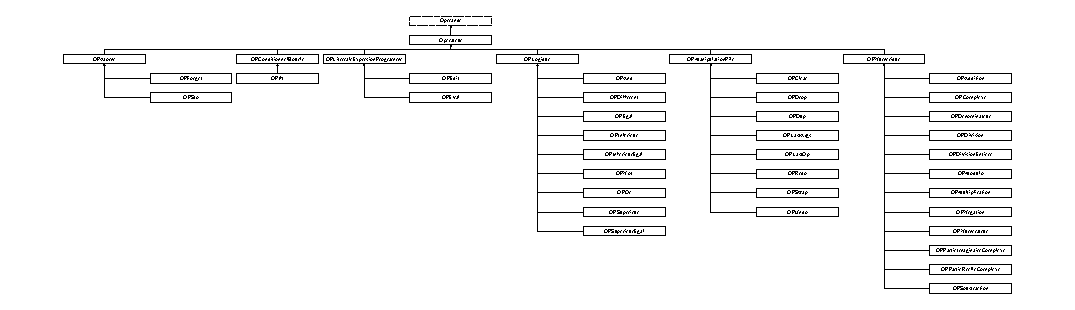
\includegraphics[height=3.725055cm]{class_operateur}
\end{center}
\end{figure}
\subsection*{Public Member Functions}
\begin{DoxyCompactItemize}
\item 
{\bfseries Operateur} (Q\+String val, int a)\hypertarget{class_operateur_ad895d724b42b720a9995af241131e0d9}{}\label{class_operateur_ad895d724b42b720a9995af241131e0d9}

\item 
virtual void {\bfseries afficher} () const \hypertarget{class_operateur_a3099169b08305713cc01fb25a6966919}{}\label{class_operateur_a3099169b08305713cc01fb25a6966919}

\item 
virtual \hyperlink{class_litterale}{Litterale} $\ast$ {\bfseries compute} ()=0\hypertarget{class_operateur_a928858667a7ae2620e8242df28d1834f}{}\label{class_operateur_a928858667a7ae2620e8242df28d1834f}

\item 
virtual \hyperlink{class_litterale}{Litterale} $\ast$ {\bfseries compute} (\hyperlink{class_litterale}{Litterale} $\ast$l)=0\hypertarget{class_operateur_a02731b815ed3b03cec582590d014414a}{}\label{class_operateur_a02731b815ed3b03cec582590d014414a}

\item 
virtual \hyperlink{class_litterale}{Litterale} $\ast$ {\bfseries compute} (\hyperlink{class_litterale}{Litterale} $\ast$l1, \hyperlink{class_litterale}{Litterale} $\ast$l2)=0\hypertarget{class_operateur_a399b64f8edc1bd882c11205b7a734727}{}\label{class_operateur_a399b64f8edc1bd882c11205b7a734727}

\item 
int {\bfseries get\+Arite} ()\hypertarget{class_operateur_af8e33992695ad219093560aaadbaa5ee}{}\label{class_operateur_af8e33992695ad219093560aaadbaa5ee}

\item 
virtual Q\+String {\bfseries get\+Text} () const \hypertarget{class_operateur_a812bdb48e7a4a512cb5921e0a256ae91}{}\label{class_operateur_a812bdb48e7a4a512cb5921e0a256ae91}

\item 
virtual \hyperlink{class_operateur}{Operateur} $\ast$ {\bfseries clone} () const  =0\hypertarget{class_operateur_a10a8157bc85eb2ceaa8e88ff42d0cd9a}{}\label{class_operateur_a10a8157bc85eb2ceaa8e88ff42d0cd9a}

\end{DoxyCompactItemize}
\subsection*{Protected Attributes}
\begin{DoxyCompactItemize}
\item 
Q\+String {\bfseries value}\hypertarget{class_operateur_a5bca78f28e8de7848dabbb53152d549a}{}\label{class_operateur_a5bca78f28e8de7848dabbb53152d549a}

\item 
int {\bfseries arite}\hypertarget{class_operateur_a5158f9da883ae20151d9f3c5bc891bc6}{}\label{class_operateur_a5158f9da883ae20151d9f3c5bc891bc6}

\end{DoxyCompactItemize}


The documentation for this class was generated from the following file\+:\begin{DoxyCompactItemize}
\item 
operateur.\+h\end{DoxyCompactItemize}

\hypertarget{class_o_p_eval}{}\section{O\+P\+Eval Class Reference}
\label{class_o_p_eval}\index{O\+P\+Eval@{O\+P\+Eval}}
Inheritance diagram for O\+P\+Eval\+:\begin{figure}[H]
\begin{center}
\leavevmode
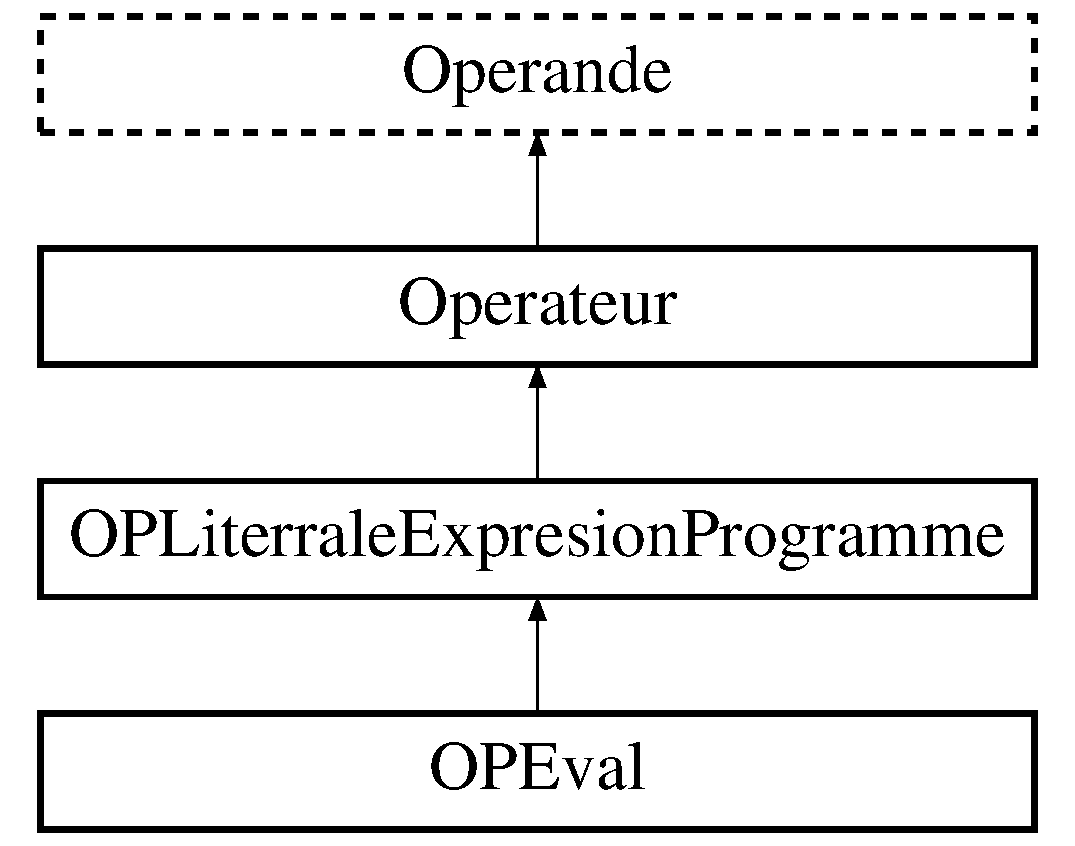
\includegraphics[height=4.000000cm]{class_o_p_eval}
\end{center}
\end{figure}
\subsection*{Public Member Functions}
\begin{DoxyCompactItemize}
\item 
virtual \hyperlink{class_o_p_eval}{O\+P\+Eval} $\ast$ {\bfseries clone} () const \hypertarget{class_o_p_eval_ad1cae68bb1b51dc285188fc40ca65bf0}{}\label{class_o_p_eval_ad1cae68bb1b51dc285188fc40ca65bf0}

\item 
virtual \hyperlink{class_litterale}{Litterale} $\ast$ {\bfseries compute} ()\hypertarget{class_o_p_eval_a9b077bf839d77d85391454c8013005b3}{}\label{class_o_p_eval_a9b077bf839d77d85391454c8013005b3}

\item 
virtual \hyperlink{class_litterale}{Litterale} $\ast$ {\bfseries compute} (\hyperlink{class_litterale}{Litterale} $\ast$l)\hypertarget{class_o_p_eval_ac6a1a4756b6e241fde8e39dab5b6f2f4}{}\label{class_o_p_eval_ac6a1a4756b6e241fde8e39dab5b6f2f4}

\item 
virtual \hyperlink{class_litterale}{Litterale} $\ast$ {\bfseries compute} (\hyperlink{class_litterale}{Litterale} $\ast$l1, \hyperlink{class_litterale}{Litterale} $\ast$l2)\hypertarget{class_o_p_eval_a8dc48ac8e0f5683ca743462c61bc68de}{}\label{class_o_p_eval_a8dc48ac8e0f5683ca743462c61bc68de}

\end{DoxyCompactItemize}
\subsection*{Additional Inherited Members}


The documentation for this class was generated from the following files\+:\begin{DoxyCompactItemize}
\item 
opliterraleexpresionprogramme.\+h\item 
opliterraleexpresionprogramme.\+cpp\end{DoxyCompactItemize}

\hypertarget{class_o_p_forget}{}\section{O\+P\+Forget Class Reference}
\label{class_o_p_forget}\index{O\+P\+Forget@{O\+P\+Forget}}
Inheritance diagram for O\+P\+Forget\+:\begin{figure}[H]
\begin{center}
\leavevmode
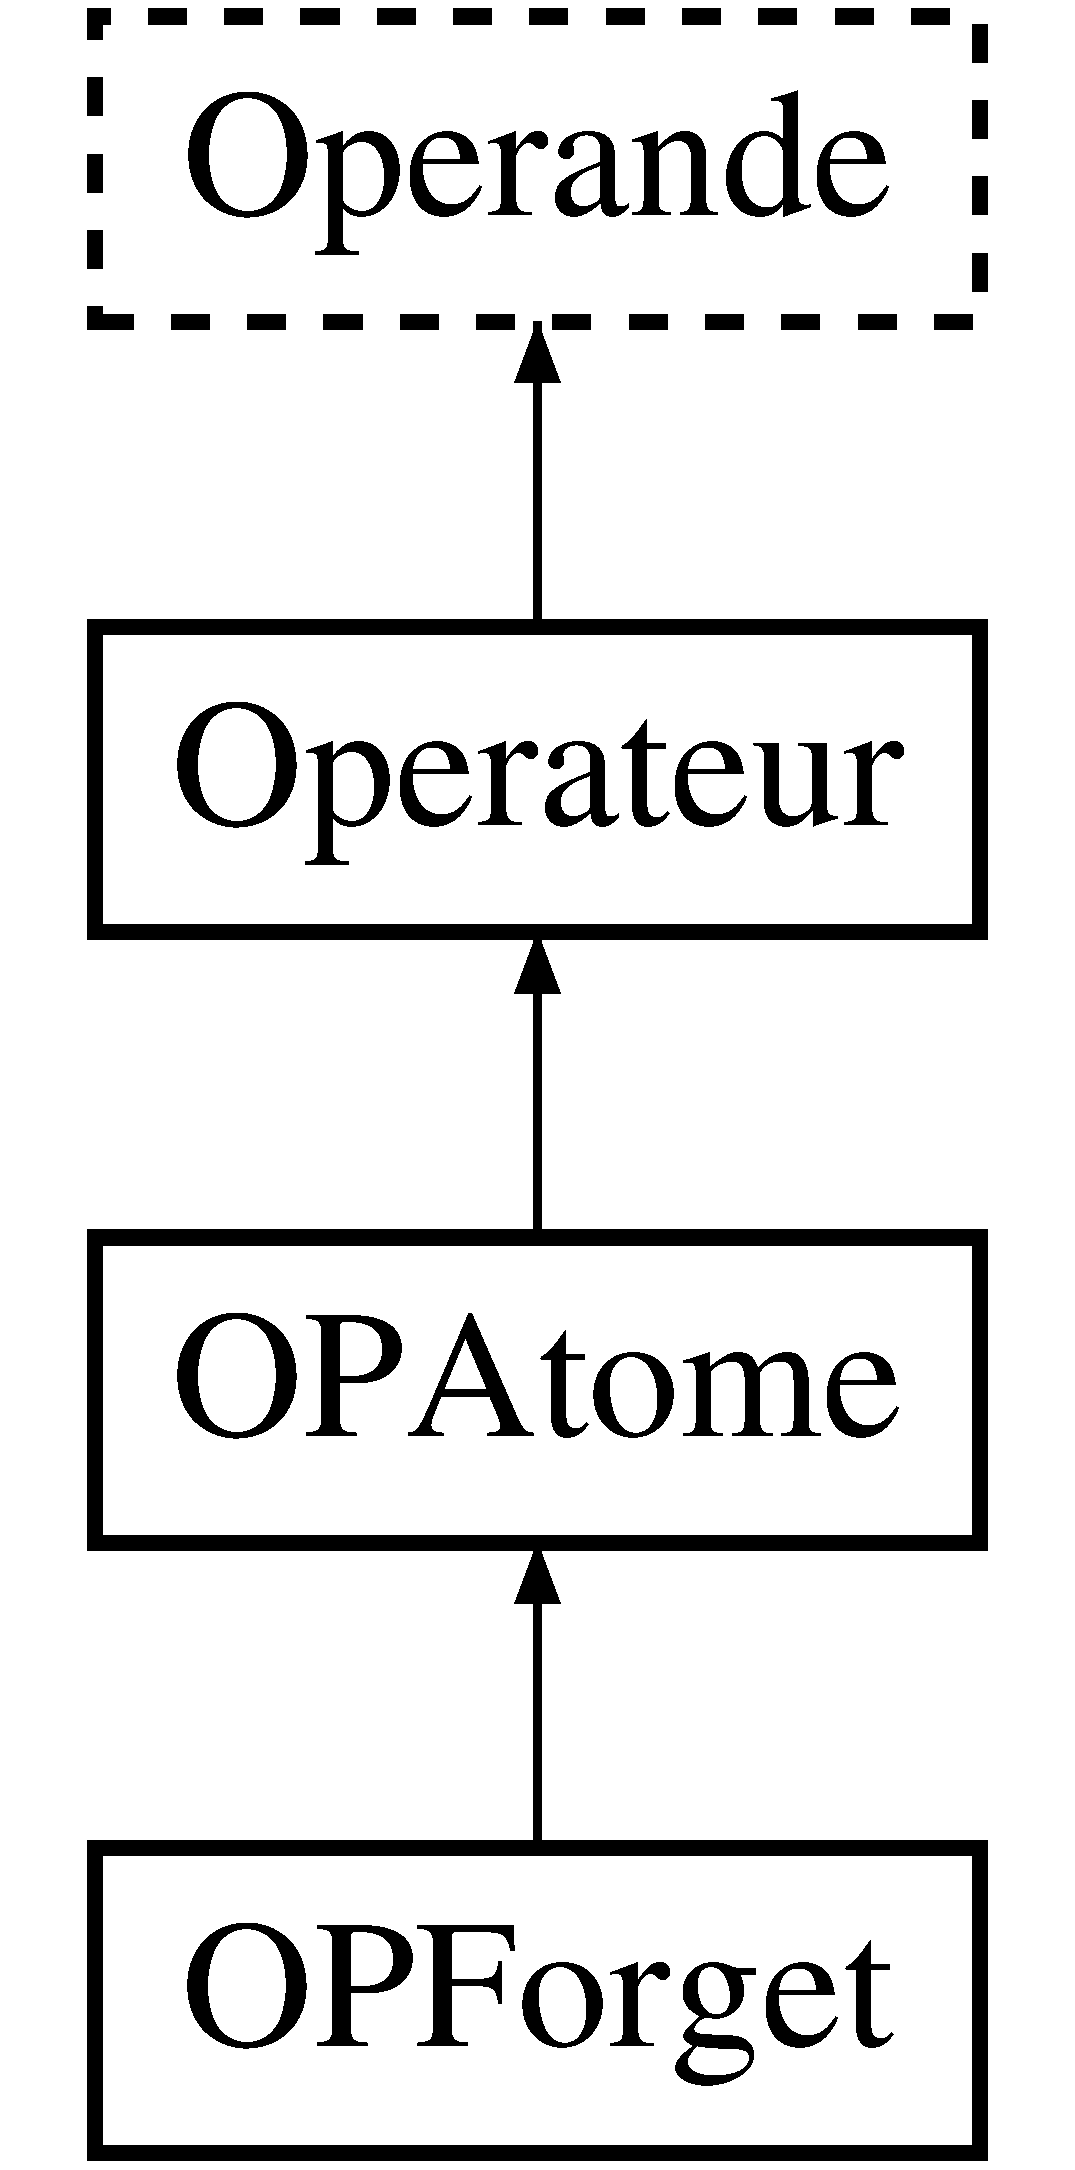
\includegraphics[height=4.000000cm]{class_o_p_forget}
\end{center}
\end{figure}
\subsection*{Public Member Functions}
\begin{DoxyCompactItemize}
\item 
virtual \hyperlink{class_o_p_forget}{O\+P\+Forget} $\ast$ {\bfseries clone} () const \hypertarget{class_o_p_forget_a2b5a61818f2a6a6124db0640b0643d56}{}\label{class_o_p_forget_a2b5a61818f2a6a6124db0640b0643d56}

\item 
virtual \hyperlink{class_litterale}{Litterale} $\ast$ {\bfseries compute} ()\hypertarget{class_o_p_forget_a2ceb2c96d61919e2b766529ea22d1901}{}\label{class_o_p_forget_a2ceb2c96d61919e2b766529ea22d1901}

\item 
virtual \hyperlink{class_litterale}{Litterale} $\ast$ {\bfseries compute} (\hyperlink{class_litterale}{Litterale} $\ast$l)\hypertarget{class_o_p_forget_a0dc97aa82ffccff2fbd59cf98824fa03}{}\label{class_o_p_forget_a0dc97aa82ffccff2fbd59cf98824fa03}

\item 
virtual \hyperlink{class_litterale}{Litterale} $\ast$ {\bfseries compute} (\hyperlink{class_litterale}{Litterale} $\ast$l1, \hyperlink{class_litterale}{Litterale} $\ast$l2)\hypertarget{class_o_p_forget_a767db9e2e60ce477a62492c46febc775}{}\label{class_o_p_forget_a767db9e2e60ce477a62492c46febc775}

\end{DoxyCompactItemize}
\subsection*{Additional Inherited Members}


The documentation for this class was generated from the following files\+:\begin{DoxyCompactItemize}
\item 
opatome.\+h\item 
opatome.\+cpp\end{DoxyCompactItemize}

\hypertarget{class_o_p_ift}{}\section{O\+P\+Ift Class Reference}
\label{class_o_p_ift}\index{O\+P\+Ift@{O\+P\+Ift}}
Inheritance diagram for O\+P\+Ift\+:\begin{figure}[H]
\begin{center}
\leavevmode
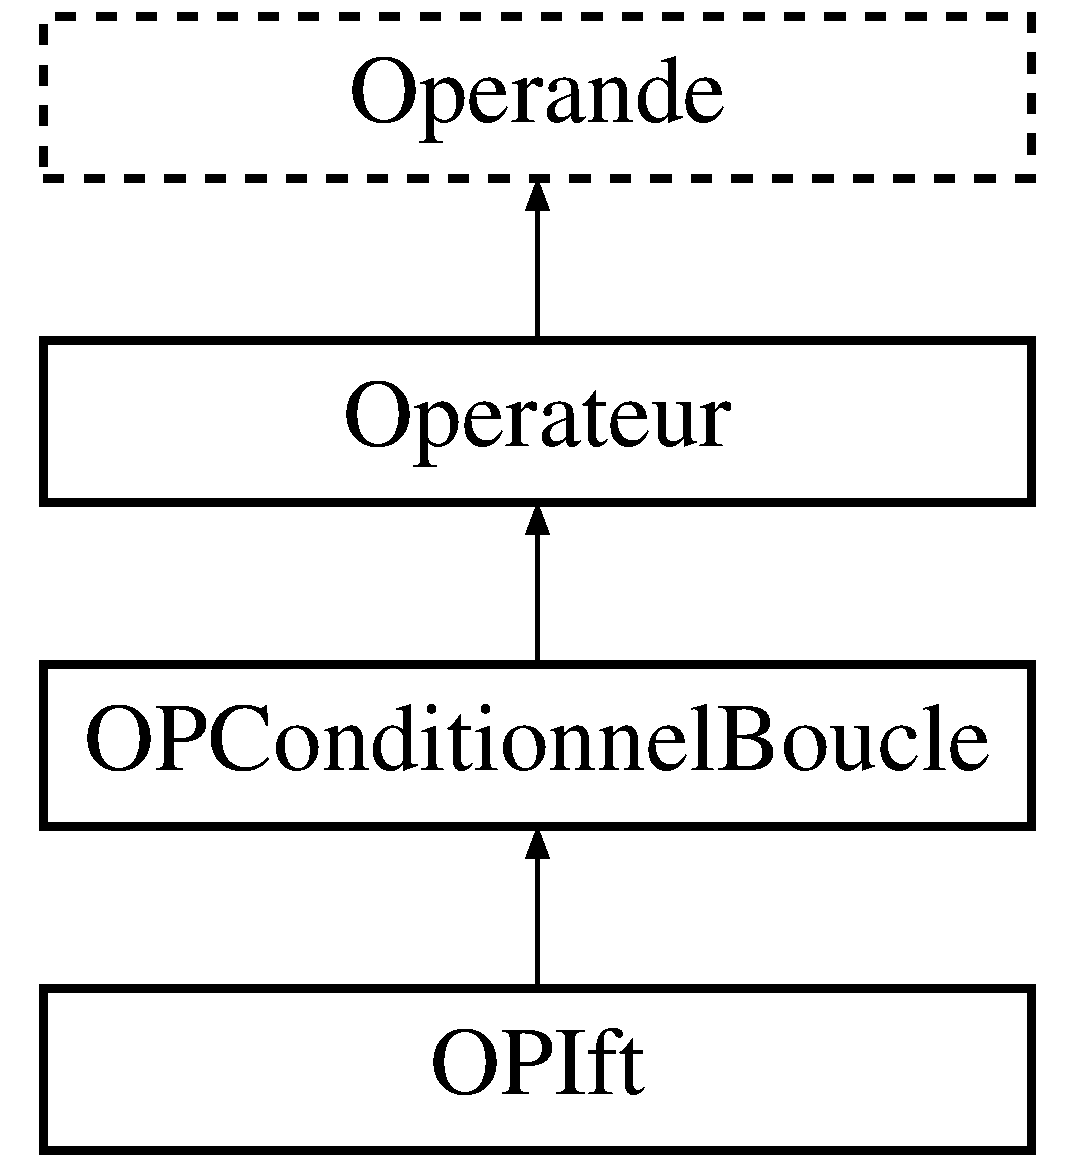
\includegraphics[height=4.000000cm]{class_o_p_ift}
\end{center}
\end{figure}
\subsection*{Public Member Functions}
\begin{DoxyCompactItemize}
\item 
virtual \hyperlink{class_o_p_ift}{O\+P\+Ift} $\ast$ {\bfseries clone} () const \hypertarget{class_o_p_ift_ae2fba0f2289ed0735850effe351d51c9}{}\label{class_o_p_ift_ae2fba0f2289ed0735850effe351d51c9}

\item 
virtual \hyperlink{class_litterale}{Litterale} $\ast$ {\bfseries compute} ()\hypertarget{class_o_p_ift_a5bd05c18e9e0786de86e1658f9835111}{}\label{class_o_p_ift_a5bd05c18e9e0786de86e1658f9835111}

\item 
virtual \hyperlink{class_litterale}{Litterale} $\ast$ {\bfseries compute} (\hyperlink{class_litterale}{Litterale} $\ast$l)\hypertarget{class_o_p_ift_a9693ee3b37a2fcf6ea34097cdd4634eb}{}\label{class_o_p_ift_a9693ee3b37a2fcf6ea34097cdd4634eb}

\item 
virtual \hyperlink{class_litterale}{Litterale} $\ast$ {\bfseries compute} (\hyperlink{class_litterale}{Litterale} $\ast$l1, \hyperlink{class_litterale}{Litterale} $\ast$l2)\hypertarget{class_o_p_ift_a1bfd149f76aa1f87b47d320fc16f12bb}{}\label{class_o_p_ift_a1bfd149f76aa1f87b47d320fc16f12bb}

\end{DoxyCompactItemize}
\subsection*{Additional Inherited Members}


The documentation for this class was generated from the following files\+:\begin{DoxyCompactItemize}
\item 
opconditionnelboucle.\+h\item 
opconditionnelboucle.\+cpp\end{DoxyCompactItemize}

\hypertarget{class_o_p_inferieur}{}\section{O\+P\+Inferieur Class Reference}
\label{class_o_p_inferieur}\index{O\+P\+Inferieur@{O\+P\+Inferieur}}
Inheritance diagram for O\+P\+Inferieur\+:\begin{figure}[H]
\begin{center}
\leavevmode
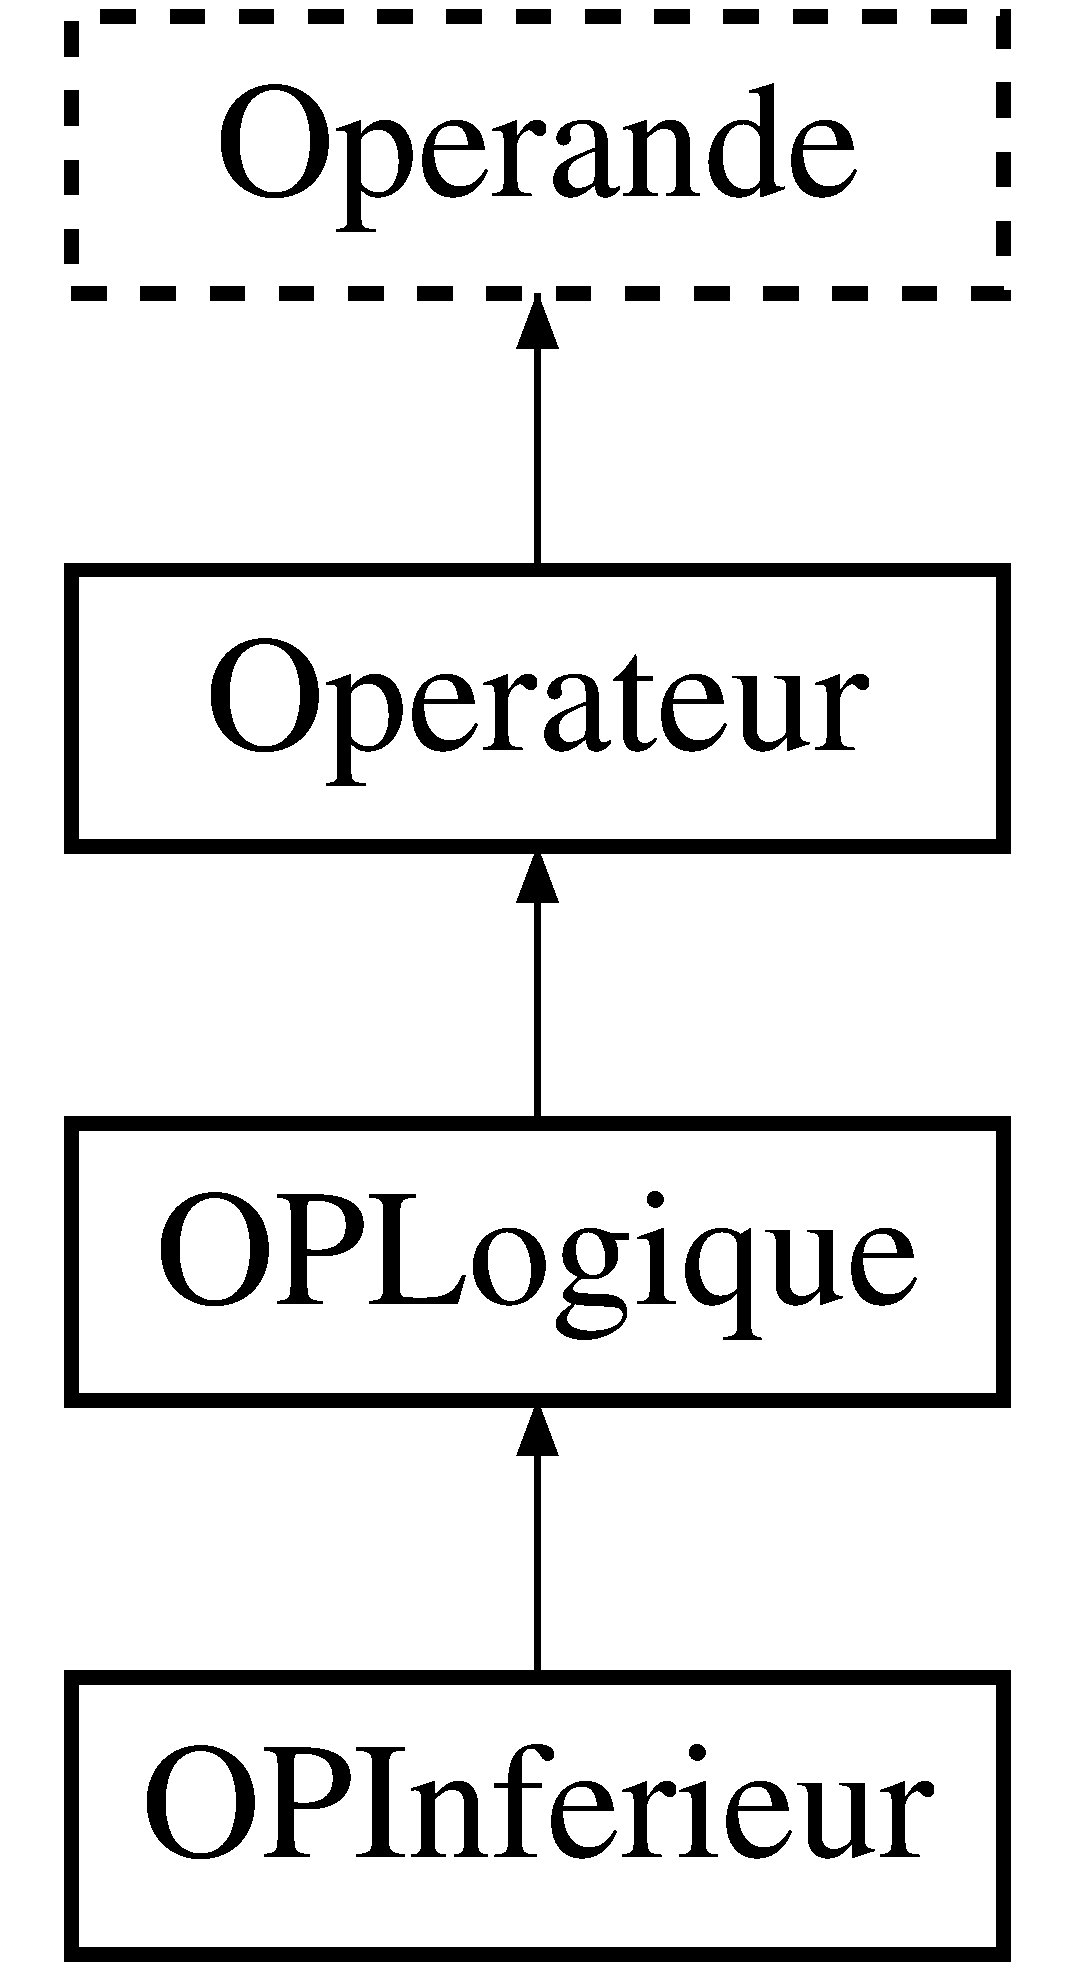
\includegraphics[height=4.000000cm]{class_o_p_inferieur}
\end{center}
\end{figure}
\subsection*{Public Member Functions}
\begin{DoxyCompactItemize}
\item 
virtual \hyperlink{class_o_p_inferieur}{O\+P\+Inferieur} $\ast$ {\bfseries clone} () const \hypertarget{class_o_p_inferieur_a953a344135f81c92cd4d6895ebf74f1e}{}\label{class_o_p_inferieur_a953a344135f81c92cd4d6895ebf74f1e}

\item 
virtual \hyperlink{class_litterale}{Litterale} $\ast$ {\bfseries compute} ()\hypertarget{class_o_p_inferieur_a826fc72202c572a0860f143ebecb841c}{}\label{class_o_p_inferieur_a826fc72202c572a0860f143ebecb841c}

\item 
virtual \hyperlink{class_litterale}{Litterale} $\ast$ {\bfseries compute} (\hyperlink{class_litterale}{Litterale} $\ast$l)\hypertarget{class_o_p_inferieur_a1efec2ac3cfd59e28af99b37017bfef2}{}\label{class_o_p_inferieur_a1efec2ac3cfd59e28af99b37017bfef2}

\item 
virtual \hyperlink{class_litterale}{Litterale} $\ast$ {\bfseries compute} (\hyperlink{class_litterale}{Litterale} $\ast$l1, \hyperlink{class_litterale}{Litterale} $\ast$l2)\hypertarget{class_o_p_inferieur_a14b11dc8649984659b2b7ec1bd9d7aa8}{}\label{class_o_p_inferieur_a14b11dc8649984659b2b7ec1bd9d7aa8}

\end{DoxyCompactItemize}
\subsection*{Additional Inherited Members}


The documentation for this class was generated from the following files\+:\begin{DoxyCompactItemize}
\item 
oplogique.\+h\item 
oplogique.\+cpp\end{DoxyCompactItemize}

\hypertarget{class_o_p_inferieur_egal}{}\section{O\+P\+Inferieur\+Egal Class Reference}
\label{class_o_p_inferieur_egal}\index{O\+P\+Inferieur\+Egal@{O\+P\+Inferieur\+Egal}}
Inheritance diagram for O\+P\+Inferieur\+Egal\+:\begin{figure}[H]
\begin{center}
\leavevmode
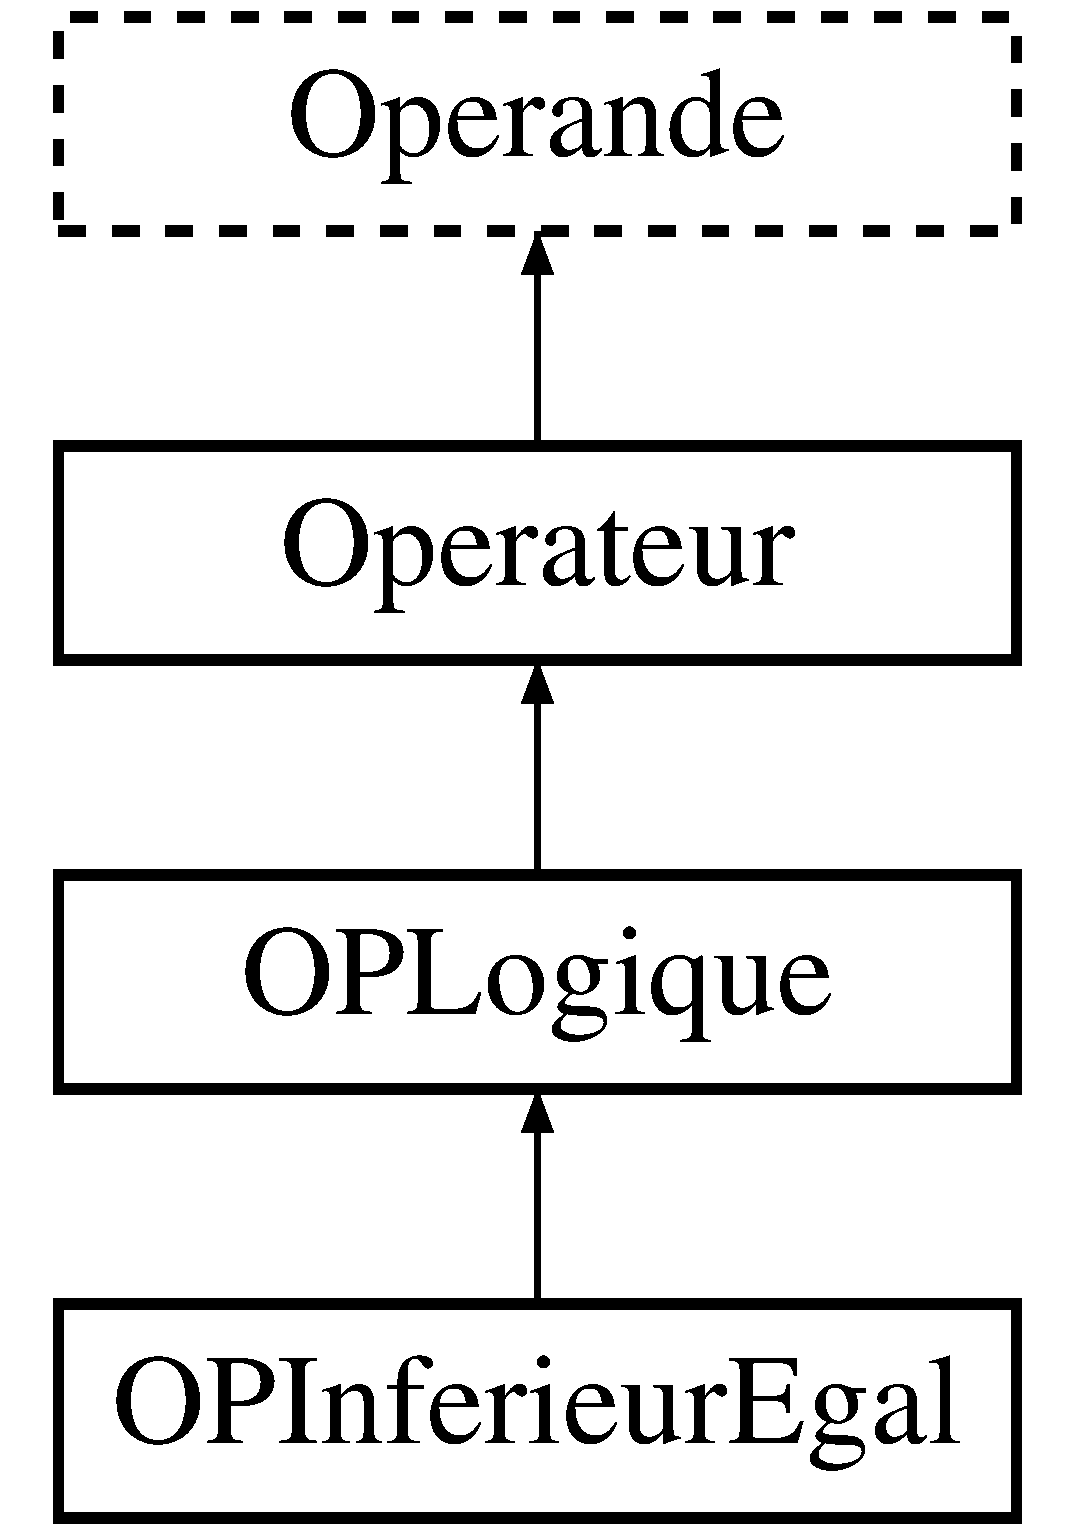
\includegraphics[height=4.000000cm]{class_o_p_inferieur_egal}
\end{center}
\end{figure}
\subsection*{Public Member Functions}
\begin{DoxyCompactItemize}
\item 
virtual \hyperlink{class_o_p_inferieur_egal}{O\+P\+Inferieur\+Egal} $\ast$ {\bfseries clone} () const \hypertarget{class_o_p_inferieur_egal_a88d147ea2add1d91572caef89bb78b2a}{}\label{class_o_p_inferieur_egal_a88d147ea2add1d91572caef89bb78b2a}

\item 
virtual \hyperlink{class_litterale}{Litterale} $\ast$ {\bfseries compute} ()\hypertarget{class_o_p_inferieur_egal_ab2f17379905b3e206f7c631ec021597e}{}\label{class_o_p_inferieur_egal_ab2f17379905b3e206f7c631ec021597e}

\item 
virtual \hyperlink{class_litterale}{Litterale} $\ast$ {\bfseries compute} (\hyperlink{class_litterale}{Litterale} $\ast$l)\hypertarget{class_o_p_inferieur_egal_a7b466750a13944c3f5d3daae7fafa797}{}\label{class_o_p_inferieur_egal_a7b466750a13944c3f5d3daae7fafa797}

\item 
virtual \hyperlink{class_litterale}{Litterale} $\ast$ {\bfseries compute} (\hyperlink{class_litterale}{Litterale} $\ast$l1, \hyperlink{class_litterale}{Litterale} $\ast$l2)\hypertarget{class_o_p_inferieur_egal_aa0d7bb26bbecdab3b19811a58e8caf78}{}\label{class_o_p_inferieur_egal_aa0d7bb26bbecdab3b19811a58e8caf78}

\end{DoxyCompactItemize}
\subsection*{Additional Inherited Members}


The documentation for this class was generated from the following files\+:\begin{DoxyCompactItemize}
\item 
oplogique.\+h\item 
oplogique.\+cpp\end{DoxyCompactItemize}

\hypertarget{class_o_p_last_args}{}\section{O\+P\+Last\+Args Class Reference}
\label{class_o_p_last_args}\index{O\+P\+Last\+Args@{O\+P\+Last\+Args}}
Inheritance diagram for O\+P\+Last\+Args\+:\begin{figure}[H]
\begin{center}
\leavevmode
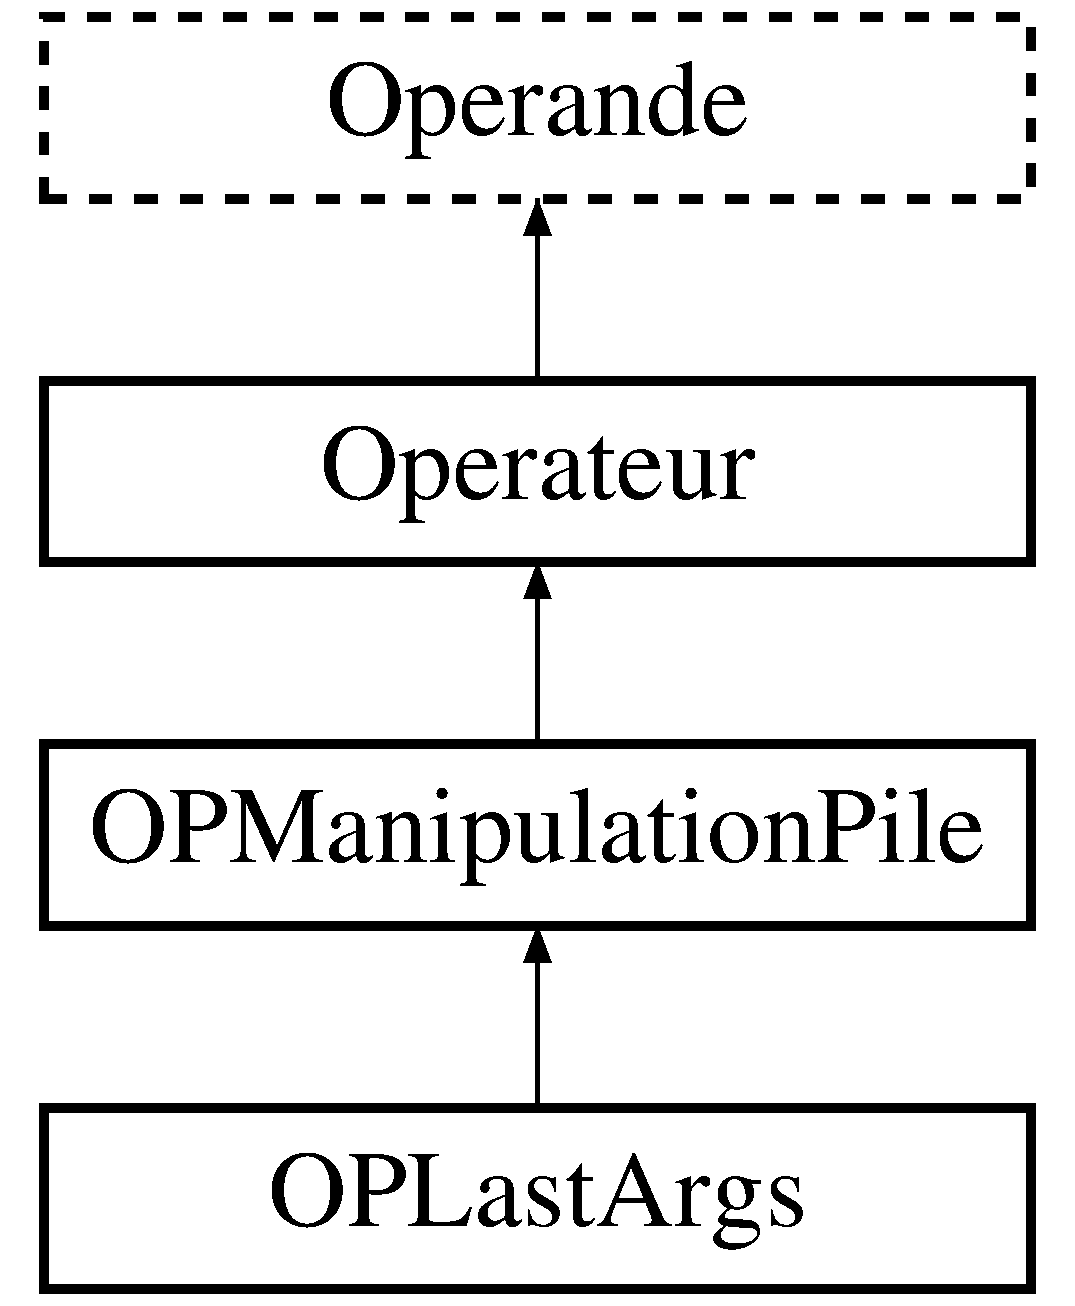
\includegraphics[height=4.000000cm]{class_o_p_last_args}
\end{center}
\end{figure}
\subsection*{Public Member Functions}
\begin{DoxyCompactItemize}
\item 
virtual \hyperlink{class_o_p_last_args}{O\+P\+Last\+Args} $\ast$ {\bfseries clone} () const \hypertarget{class_o_p_last_args_a4ef41f82d64ffa665ec4b3576730c35a}{}\label{class_o_p_last_args_a4ef41f82d64ffa665ec4b3576730c35a}

\item 
virtual \hyperlink{class_litterale}{Litterale} $\ast$ {\bfseries compute} ()\hypertarget{class_o_p_last_args_a3f532d3d087339d26c18e6acbab7ebe0}{}\label{class_o_p_last_args_a3f532d3d087339d26c18e6acbab7ebe0}

\item 
virtual \hyperlink{class_litterale}{Litterale} $\ast$ {\bfseries compute} (\hyperlink{class_litterale}{Litterale} $\ast$l)\hypertarget{class_o_p_last_args_a0c4b0474ac13e1d56a6cecf1f6970e49}{}\label{class_o_p_last_args_a0c4b0474ac13e1d56a6cecf1f6970e49}

\item 
virtual \hyperlink{class_litterale}{Litterale} $\ast$ {\bfseries compute} (\hyperlink{class_litterale}{Litterale} $\ast$l1, \hyperlink{class_litterale}{Litterale} $\ast$l2)\hypertarget{class_o_p_last_args_a194a34c7b79a102b9d7e4a81743c5050}{}\label{class_o_p_last_args_a194a34c7b79a102b9d7e4a81743c5050}

\end{DoxyCompactItemize}
\subsection*{Additional Inherited Members}


The documentation for this class was generated from the following files\+:\begin{DoxyCompactItemize}
\item 
opmanipulationpile.\+h\item 
opmanipulationpile.\+cpp\end{DoxyCompactItemize}

\hypertarget{class_o_p_last_op}{}\section{O\+P\+Last\+Op Class Reference}
\label{class_o_p_last_op}\index{O\+P\+Last\+Op@{O\+P\+Last\+Op}}
Inheritance diagram for O\+P\+Last\+Op\+:\begin{figure}[H]
\begin{center}
\leavevmode
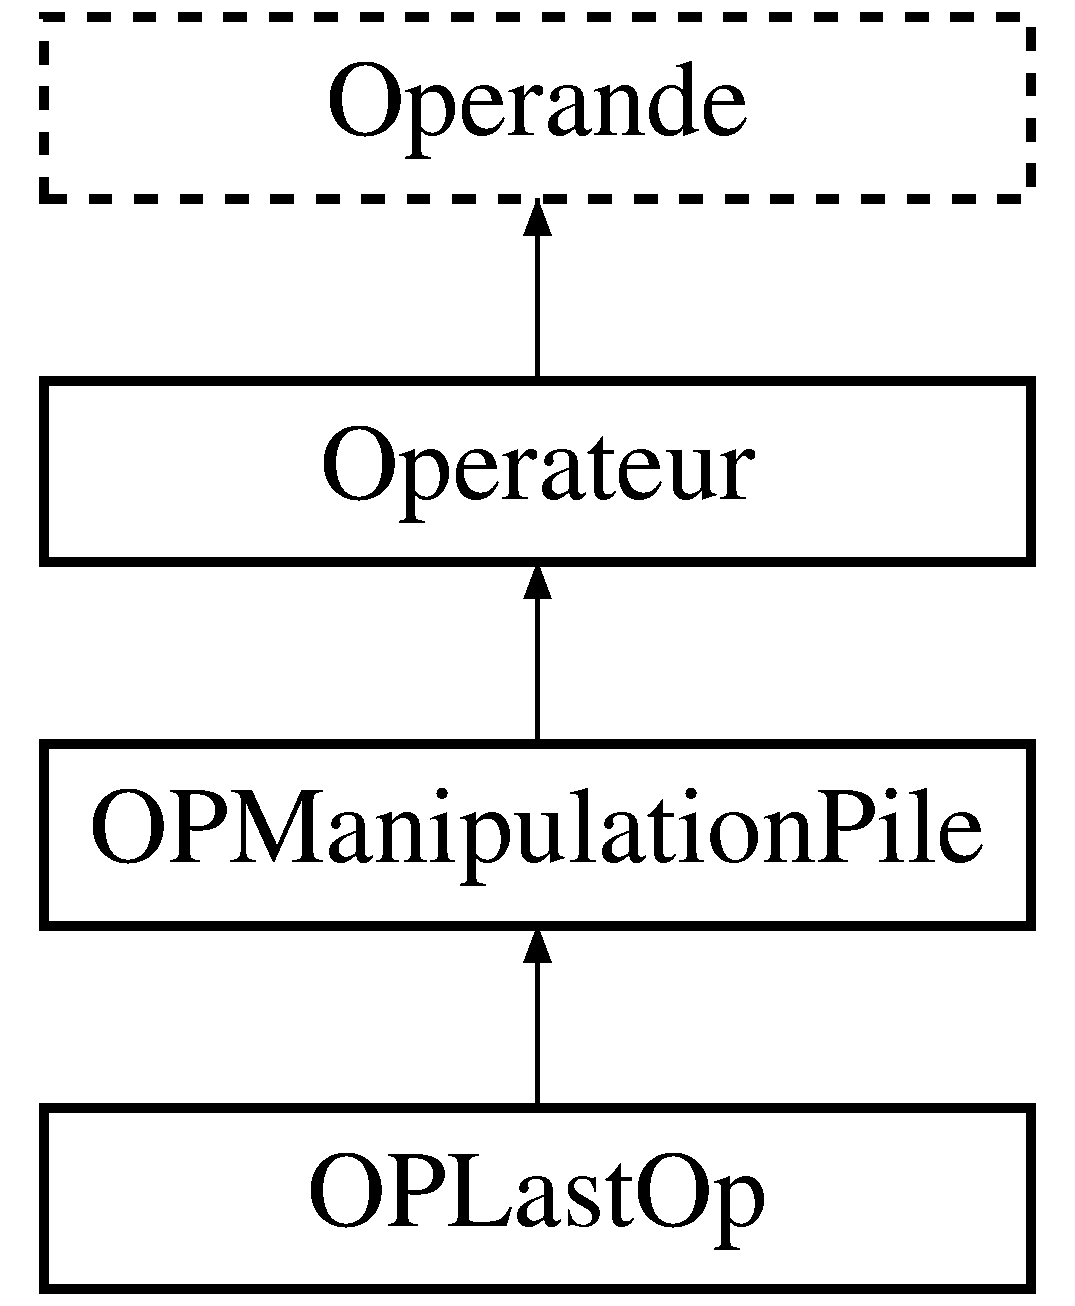
\includegraphics[height=4.000000cm]{class_o_p_last_op}
\end{center}
\end{figure}
\subsection*{Public Member Functions}
\begin{DoxyCompactItemize}
\item 
virtual \hyperlink{class_o_p_last_op}{O\+P\+Last\+Op} $\ast$ {\bfseries clone} () const \hypertarget{class_o_p_last_op_a3209e7ea84a78ebc66514584b4865eef}{}\label{class_o_p_last_op_a3209e7ea84a78ebc66514584b4865eef}

\item 
virtual \hyperlink{class_litterale}{Litterale} $\ast$ {\bfseries compute} ()\hypertarget{class_o_p_last_op_a0692f09d3cf4cd2cc47cd7243f828cd0}{}\label{class_o_p_last_op_a0692f09d3cf4cd2cc47cd7243f828cd0}

\item 
virtual \hyperlink{class_litterale}{Litterale} $\ast$ {\bfseries compute} (\hyperlink{class_litterale}{Litterale} $\ast$l)\hypertarget{class_o_p_last_op_a1d219fab79fa80fa2cb58ecaac499b8a}{}\label{class_o_p_last_op_a1d219fab79fa80fa2cb58ecaac499b8a}

\item 
virtual \hyperlink{class_litterale}{Litterale} $\ast$ {\bfseries compute} (\hyperlink{class_litterale}{Litterale} $\ast$l1, \hyperlink{class_litterale}{Litterale} $\ast$l2)\hypertarget{class_o_p_last_op_a89b23f190a0e36cbbcfe8824ef620469}{}\label{class_o_p_last_op_a89b23f190a0e36cbbcfe8824ef620469}

\end{DoxyCompactItemize}
\subsection*{Additional Inherited Members}


The documentation for this class was generated from the following files\+:\begin{DoxyCompactItemize}
\item 
opmanipulationpile.\+h\item 
opmanipulationpile.\+cpp\end{DoxyCompactItemize}

\hypertarget{class_o_p_literrale_expresion_programme}{}\section{O\+P\+Literrale\+Expresion\+Programme Class Reference}
\label{class_o_p_literrale_expresion_programme}\index{O\+P\+Literrale\+Expresion\+Programme@{O\+P\+Literrale\+Expresion\+Programme}}
Inheritance diagram for O\+P\+Literrale\+Expresion\+Programme\+:\begin{figure}[H]
\begin{center}
\leavevmode
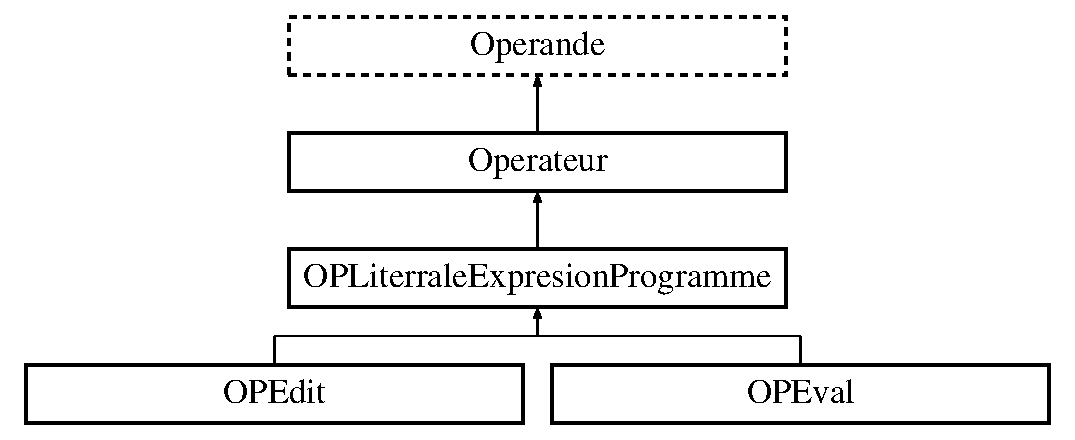
\includegraphics[height=4.000000cm]{class_o_p_literrale_expresion_programme}
\end{center}
\end{figure}
\subsection*{Public Member Functions}
\begin{DoxyCompactItemize}
\item 
{\bfseries O\+P\+Literrale\+Expresion\+Programme} (Q\+String val, int a)\hypertarget{class_o_p_literrale_expresion_programme_a2da09e01e37ec756976bc910bbcb799a}{}\label{class_o_p_literrale_expresion_programme_a2da09e01e37ec756976bc910bbcb799a}

\item 
virtual \hyperlink{class_o_p_literrale_expresion_programme}{O\+P\+Literrale\+Expresion\+Programme} $\ast$ {\bfseries clone} () const  =0\hypertarget{class_o_p_literrale_expresion_programme_a7172e6b3d9d2849dcc220085ae5d8316}{}\label{class_o_p_literrale_expresion_programme_a7172e6b3d9d2849dcc220085ae5d8316}

\item 
virtual \hyperlink{class_litterale}{Litterale} $\ast$ {\bfseries compute} ()=0\hypertarget{class_o_p_literrale_expresion_programme_ae6b8a97924a17ec536a2f810beb0ee01}{}\label{class_o_p_literrale_expresion_programme_ae6b8a97924a17ec536a2f810beb0ee01}

\item 
virtual \hyperlink{class_litterale}{Litterale} $\ast$ {\bfseries compute} (\hyperlink{class_litterale}{Litterale} $\ast$l)=0\hypertarget{class_o_p_literrale_expresion_programme_ad763f93ec588b6b80932aee8e44e98cc}{}\label{class_o_p_literrale_expresion_programme_ad763f93ec588b6b80932aee8e44e98cc}

\item 
virtual \hyperlink{class_litterale}{Litterale} $\ast$ {\bfseries compute} (\hyperlink{class_litterale}{Litterale} $\ast$l1, \hyperlink{class_litterale}{Litterale} $\ast$l2)=0\hypertarget{class_o_p_literrale_expresion_programme_a3a2fb496deae841a35adef5194d61aed}{}\label{class_o_p_literrale_expresion_programme_a3a2fb496deae841a35adef5194d61aed}

\end{DoxyCompactItemize}
\subsection*{Additional Inherited Members}


The documentation for this class was generated from the following file\+:\begin{DoxyCompactItemize}
\item 
opliterraleexpresionprogramme.\+h\end{DoxyCompactItemize}

\hypertarget{class_o_p_logique}{}\section{O\+P\+Logique Class Reference}
\label{class_o_p_logique}\index{O\+P\+Logique@{O\+P\+Logique}}
Inheritance diagram for O\+P\+Logique\+:\begin{figure}[H]
\begin{center}
\leavevmode
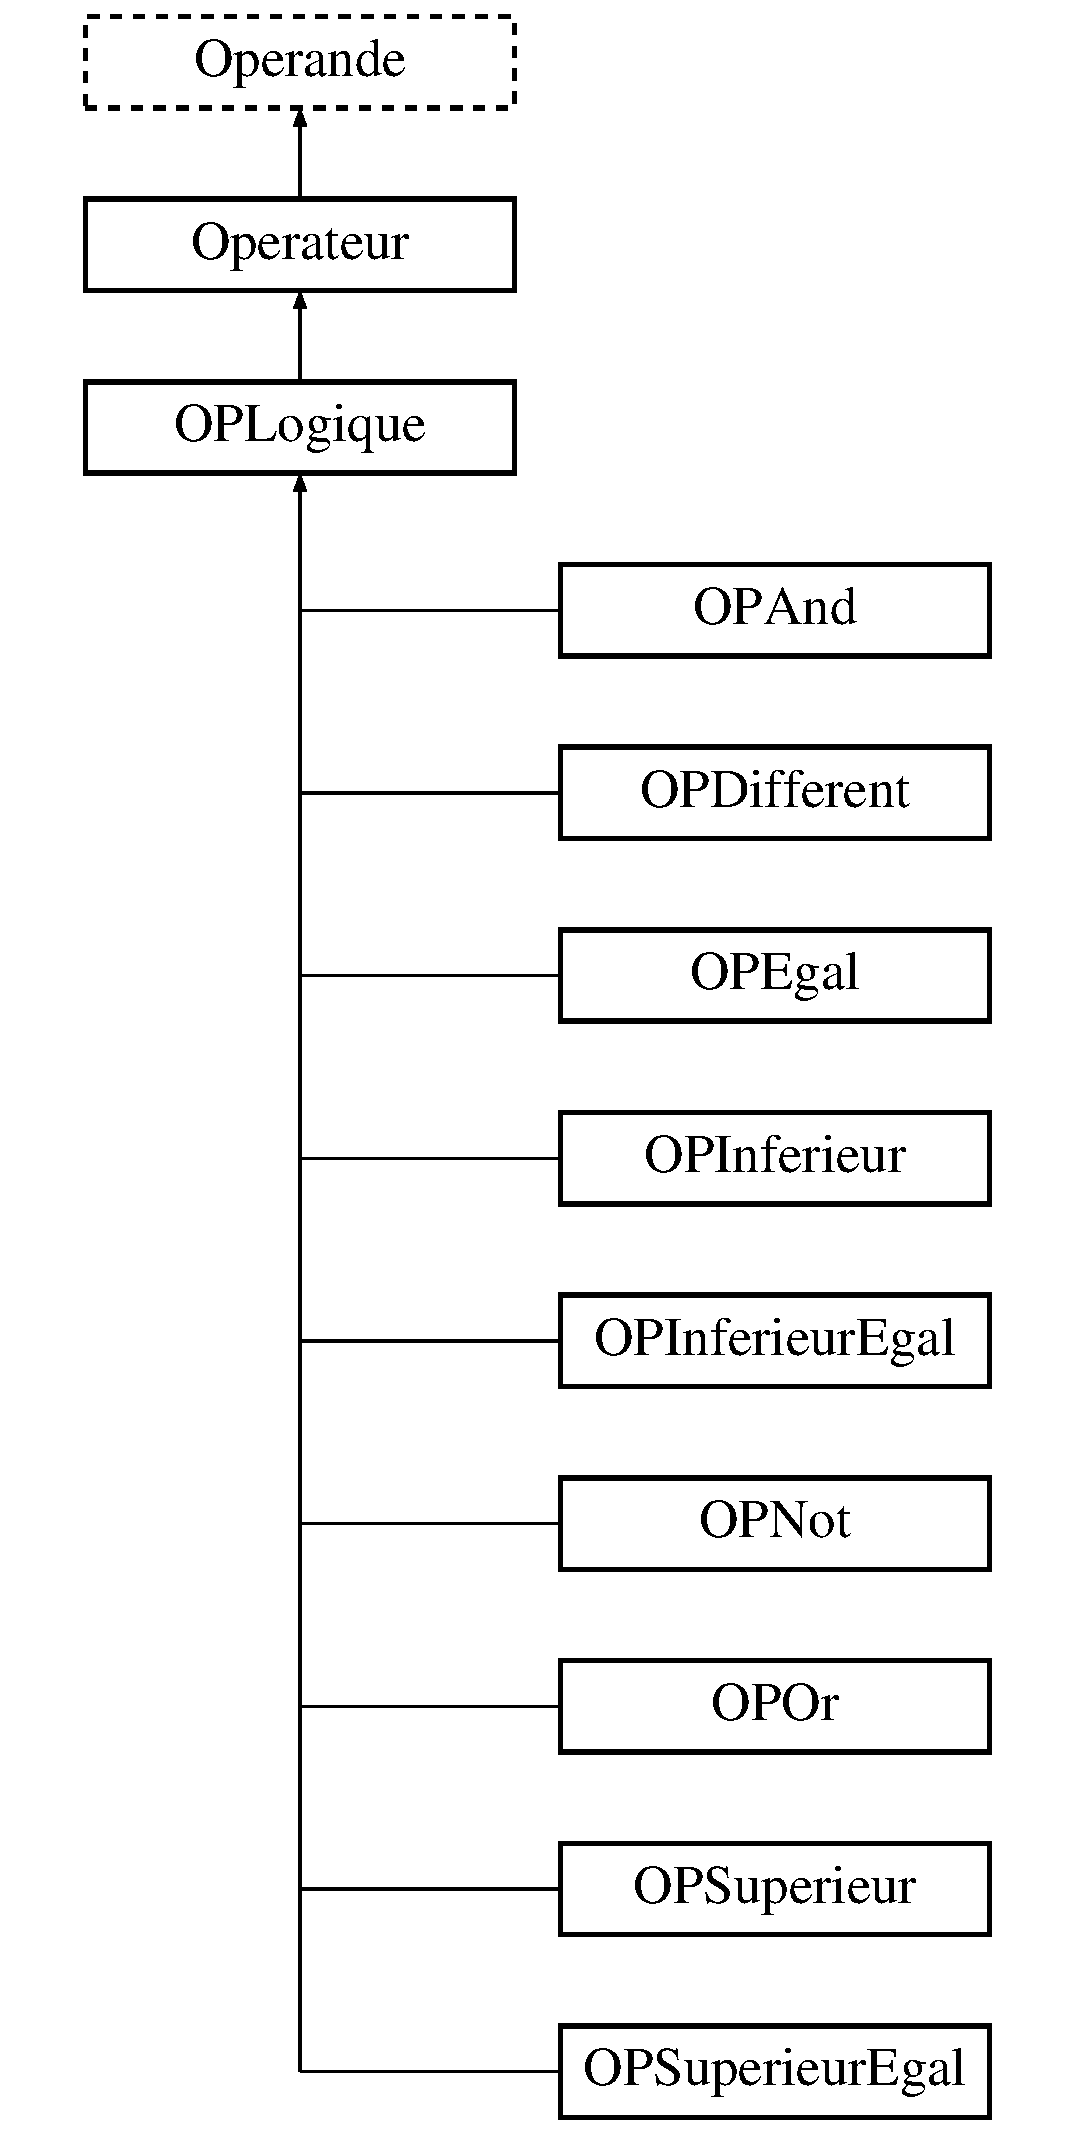
\includegraphics[height=12.000000cm]{class_o_p_logique}
\end{center}
\end{figure}
\subsection*{Public Member Functions}
\begin{DoxyCompactItemize}
\item 
{\bfseries O\+P\+Logique} (Q\+String val, int a)\hypertarget{class_o_p_logique_a38e1e9c66c277efbfb94170f86125946}{}\label{class_o_p_logique_a38e1e9c66c277efbfb94170f86125946}

\item 
virtual \hyperlink{class_o_p_logique}{O\+P\+Logique} $\ast$ {\bfseries clone} () const  =0\hypertarget{class_o_p_logique_a4ea4669b0167724dcfa6e5919560214c}{}\label{class_o_p_logique_a4ea4669b0167724dcfa6e5919560214c}

\item 
virtual \hyperlink{class_litterale}{Litterale} $\ast$ {\bfseries compute} ()=0\hypertarget{class_o_p_logique_a2c8b58eb448f57fec28785fbe8118c64}{}\label{class_o_p_logique_a2c8b58eb448f57fec28785fbe8118c64}

\item 
virtual \hyperlink{class_litterale}{Litterale} $\ast$ {\bfseries compute} (\hyperlink{class_litterale}{Litterale} $\ast$l)=0\hypertarget{class_o_p_logique_a0077e7dd288f03fe71dd4b948a7703c8}{}\label{class_o_p_logique_a0077e7dd288f03fe71dd4b948a7703c8}

\item 
virtual \hyperlink{class_litterale}{Litterale} $\ast$ {\bfseries compute} (\hyperlink{class_litterale}{Litterale} $\ast$l1, \hyperlink{class_litterale}{Litterale} $\ast$l2)=0\hypertarget{class_o_p_logique_aa29609988592fc385df0ff2ea6c7813d}{}\label{class_o_p_logique_aa29609988592fc385df0ff2ea6c7813d}

\end{DoxyCompactItemize}
\subsection*{Static Public Attributes}
\begin{DoxyCompactItemize}
\item 
static const \hyperlink{class_l_t_entier}{L\+T\+Entier} {\bfseries true\+Value} = \hyperlink{class_l_t_entier}{L\+T\+Entier}(1)\hypertarget{class_o_p_logique_a7d3a0ae1fe39b29c353a32e2dbbca575}{}\label{class_o_p_logique_a7d3a0ae1fe39b29c353a32e2dbbca575}

\item 
static const \hyperlink{class_l_t_entier}{L\+T\+Entier} {\bfseries false\+Value} = \hyperlink{class_l_t_entier}{L\+T\+Entier}(0)\hypertarget{class_o_p_logique_afb2af55eef8d0bc62494b8654bf3f949}{}\label{class_o_p_logique_afb2af55eef8d0bc62494b8654bf3f949}

\end{DoxyCompactItemize}
\subsection*{Additional Inherited Members}


The documentation for this class was generated from the following files\+:\begin{DoxyCompactItemize}
\item 
oplogique.\+h\item 
oplogique.\+cpp\end{DoxyCompactItemize}

\hypertarget{class_o_p_manipulation_pile}{}\section{O\+P\+Manipulation\+Pile Class Reference}
\label{class_o_p_manipulation_pile}\index{O\+P\+Manipulation\+Pile@{O\+P\+Manipulation\+Pile}}
Inheritance diagram for O\+P\+Manipulation\+Pile\+:\begin{figure}[H]
\begin{center}
\leavevmode
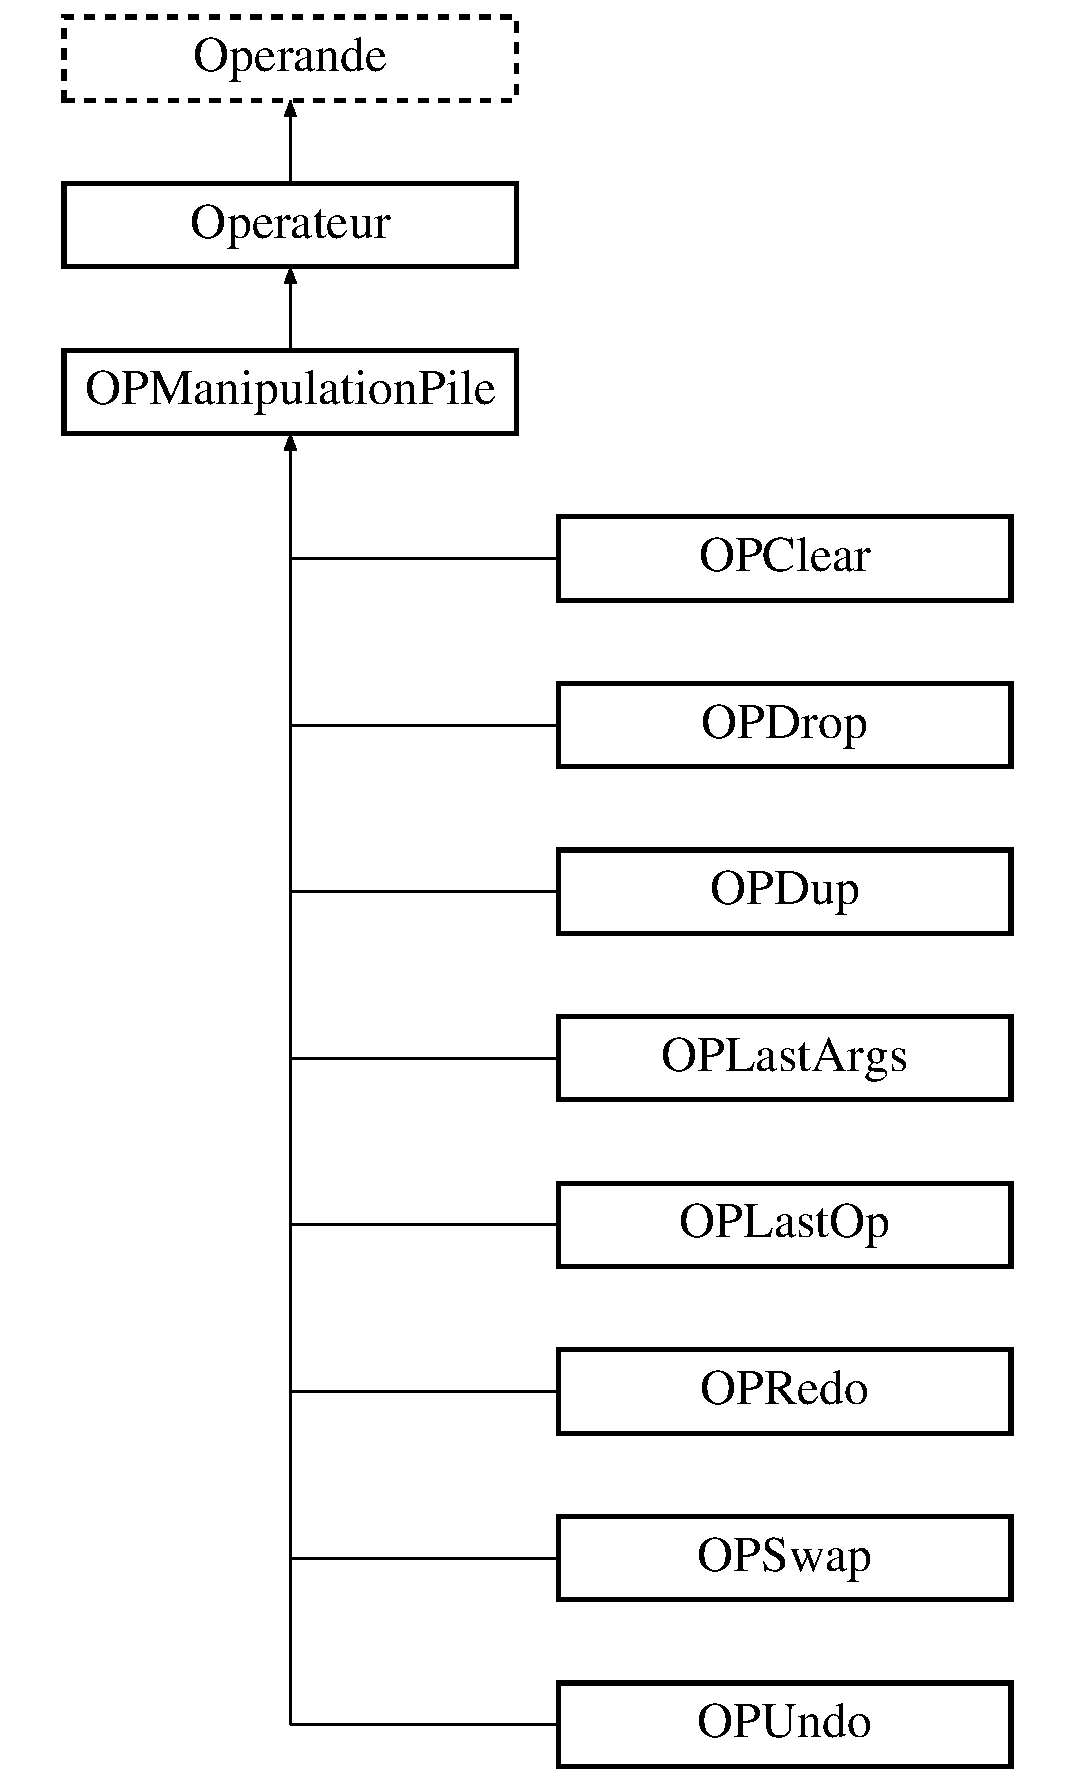
\includegraphics[height=11.000000cm]{class_o_p_manipulation_pile}
\end{center}
\end{figure}
\subsection*{Public Member Functions}
\begin{DoxyCompactItemize}
\item 
{\bfseries O\+P\+Manipulation\+Pile} (Q\+String val, int a)\hypertarget{class_o_p_manipulation_pile_a359e8ef737c1b4f312e351d7b401edef}{}\label{class_o_p_manipulation_pile_a359e8ef737c1b4f312e351d7b401edef}

\item 
virtual \hyperlink{class_o_p_manipulation_pile}{O\+P\+Manipulation\+Pile} $\ast$ {\bfseries clone} () const  =0\hypertarget{class_o_p_manipulation_pile_ac67c53b033b086749a6da773093fb9ea}{}\label{class_o_p_manipulation_pile_ac67c53b033b086749a6da773093fb9ea}

\item 
virtual \hyperlink{class_litterale}{Litterale} $\ast$ {\bfseries compute} ()=0\hypertarget{class_o_p_manipulation_pile_a9b1b4774ca2d3561a64a9c7bdb0c29ca}{}\label{class_o_p_manipulation_pile_a9b1b4774ca2d3561a64a9c7bdb0c29ca}

\item 
virtual \hyperlink{class_litterale}{Litterale} $\ast$ {\bfseries compute} (\hyperlink{class_litterale}{Litterale} $\ast$l)=0\hypertarget{class_o_p_manipulation_pile_a689328e01162aca9bbf1f41173caf2b8}{}\label{class_o_p_manipulation_pile_a689328e01162aca9bbf1f41173caf2b8}

\item 
virtual \hyperlink{class_litterale}{Litterale} $\ast$ {\bfseries compute} (\hyperlink{class_litterale}{Litterale} $\ast$l1, \hyperlink{class_litterale}{Litterale} $\ast$l2)=0\hypertarget{class_o_p_manipulation_pile_a2113dd755fb0a10cc7ed64c0f37d256f}{}\label{class_o_p_manipulation_pile_a2113dd755fb0a10cc7ed64c0f37d256f}

\end{DoxyCompactItemize}
\subsection*{Additional Inherited Members}


The documentation for this class was generated from the following file\+:\begin{DoxyCompactItemize}
\item 
opmanipulationpile.\+h\end{DoxyCompactItemize}

\hypertarget{class_o_p_modulo}{}\section{O\+P\+Modulo Class Reference}
\label{class_o_p_modulo}\index{O\+P\+Modulo@{O\+P\+Modulo}}
Inheritance diagram for O\+P\+Modulo\+:\begin{figure}[H]
\begin{center}
\leavevmode
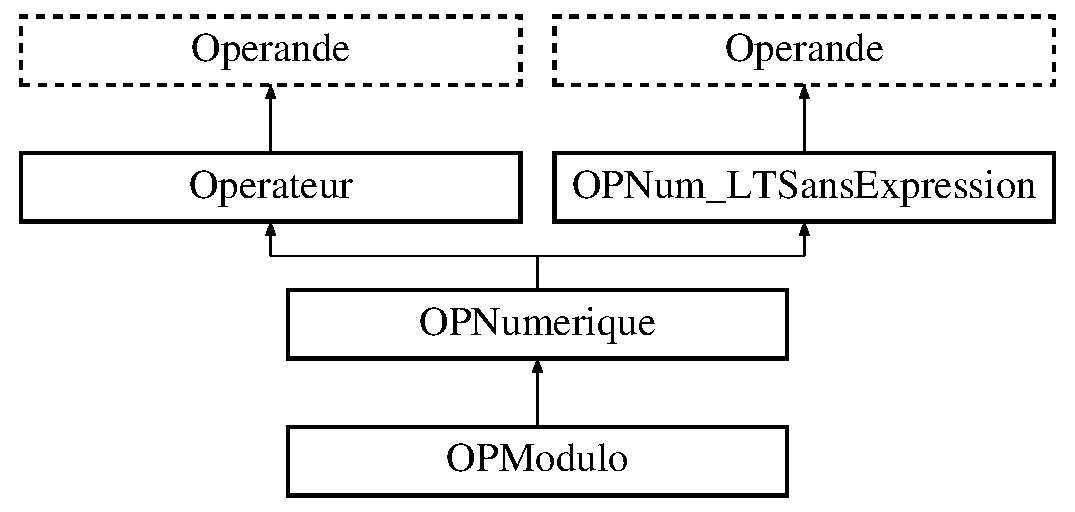
\includegraphics[height=4.000000cm]{class_o_p_modulo}
\end{center}
\end{figure}
\subsection*{Public Member Functions}
\begin{DoxyCompactItemize}
\item 
virtual \hyperlink{class_o_p_modulo}{O\+P\+Modulo} $\ast$ {\bfseries clone} () const \hypertarget{class_o_p_modulo_a1bf5d7198bd14239e1b5223923432119}{}\label{class_o_p_modulo_a1bf5d7198bd14239e1b5223923432119}

\item 
virtual \hyperlink{class_litterale}{Litterale} $\ast$ {\bfseries compute} ()\hypertarget{class_o_p_modulo_a2bb266ad934b4d5d87b07a386b25919b}{}\label{class_o_p_modulo_a2bb266ad934b4d5d87b07a386b25919b}

\item 
virtual \hyperlink{class_litterale}{Litterale} $\ast$ {\bfseries compute} (\hyperlink{class_litterale}{Litterale} $\ast$l)\hypertarget{class_o_p_modulo_af075cdef0ae0554e0d7743bb87d8846a}{}\label{class_o_p_modulo_af075cdef0ae0554e0d7743bb87d8846a}

\item 
virtual \hyperlink{class_litterale}{Litterale} $\ast$ {\bfseries compute} (\hyperlink{class_litterale}{Litterale} $\ast$l1, \hyperlink{class_litterale}{Litterale} $\ast$l2)\hypertarget{class_o_p_modulo_aff04f14ef28ce2d58718dc506f07217e}{}\label{class_o_p_modulo_aff04f14ef28ce2d58718dc506f07217e}

\end{DoxyCompactItemize}
\subsection*{Additional Inherited Members}


The documentation for this class was generated from the following files\+:\begin{DoxyCompactItemize}
\item 
opnumerique.\+h\item 
opnumerique.\+cpp\end{DoxyCompactItemize}

\hypertarget{class_o_p_multiplication}{}\section{O\+P\+Multiplication Class Reference}
\label{class_o_p_multiplication}\index{O\+P\+Multiplication@{O\+P\+Multiplication}}
Inheritance diagram for O\+P\+Multiplication\+:\begin{figure}[H]
\begin{center}
\leavevmode
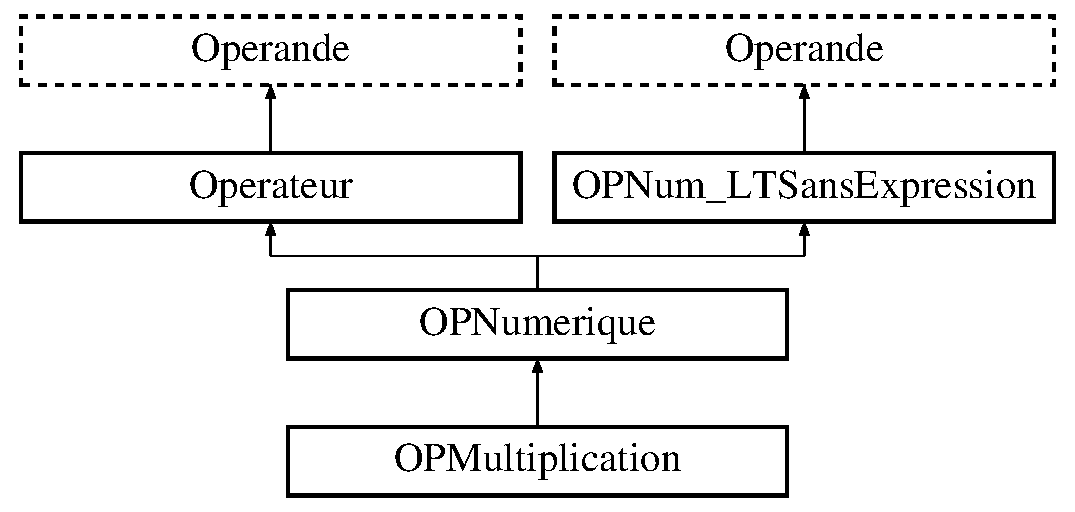
\includegraphics[height=4.000000cm]{class_o_p_multiplication}
\end{center}
\end{figure}
\subsection*{Public Member Functions}
\begin{DoxyCompactItemize}
\item 
virtual \hyperlink{class_o_p_multiplication}{O\+P\+Multiplication} $\ast$ {\bfseries clone} () const \hypertarget{class_o_p_multiplication_a66480e4938363d21b1e4a97fd3bf567a}{}\label{class_o_p_multiplication_a66480e4938363d21b1e4a97fd3bf567a}

\item 
virtual \hyperlink{class_litterale}{Litterale} $\ast$ {\bfseries compute} ()\hypertarget{class_o_p_multiplication_a7d003b8266223388ae42d7bd97743026}{}\label{class_o_p_multiplication_a7d003b8266223388ae42d7bd97743026}

\item 
virtual \hyperlink{class_litterale}{Litterale} $\ast$ {\bfseries compute} (\hyperlink{class_litterale}{Litterale} $\ast$l)\hypertarget{class_o_p_multiplication_a0df1aa4bb76cd4171a8796d330f4ed19}{}\label{class_o_p_multiplication_a0df1aa4bb76cd4171a8796d330f4ed19}

\item 
virtual \hyperlink{class_litterale}{Litterale} $\ast$ {\bfseries compute} (\hyperlink{class_litterale}{Litterale} $\ast$l1, \hyperlink{class_litterale}{Litterale} $\ast$l2)\hypertarget{class_o_p_multiplication_a7fbe82d1301bac177fa893d754beeb22}{}\label{class_o_p_multiplication_a7fbe82d1301bac177fa893d754beeb22}

\end{DoxyCompactItemize}
\subsection*{Additional Inherited Members}


The documentation for this class was generated from the following files\+:\begin{DoxyCompactItemize}
\item 
opnumerique.\+h\item 
opnumerique.\+cpp\end{DoxyCompactItemize}

\hypertarget{class_o_p_negation}{}\section{O\+P\+Negation Class Reference}
\label{class_o_p_negation}\index{O\+P\+Negation@{O\+P\+Negation}}
Inheritance diagram for O\+P\+Negation\+:\begin{figure}[H]
\begin{center}
\leavevmode
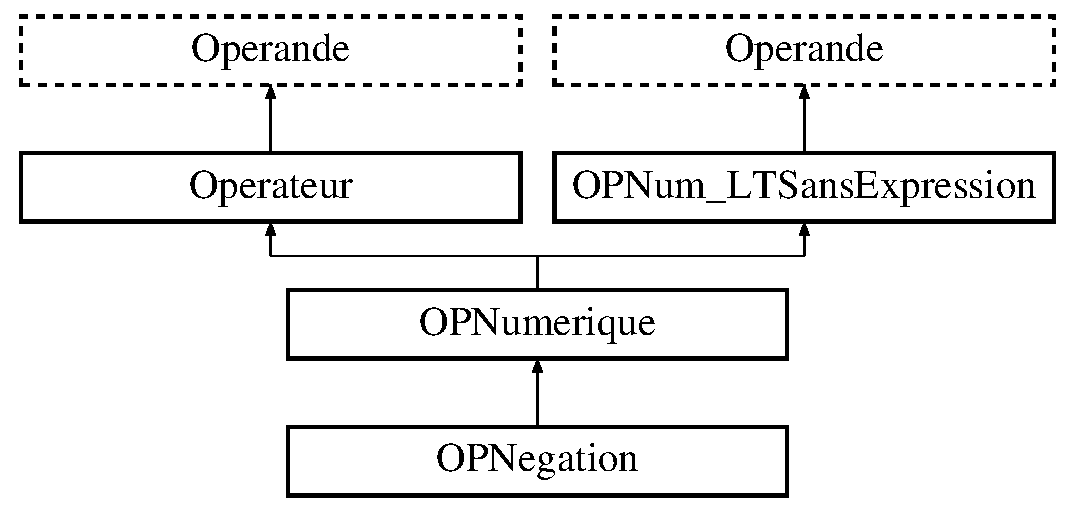
\includegraphics[height=4.000000cm]{class_o_p_negation}
\end{center}
\end{figure}
\subsection*{Public Member Functions}
\begin{DoxyCompactItemize}
\item 
virtual \hyperlink{class_o_p_negation}{O\+P\+Negation} $\ast$ {\bfseries clone} () const \hypertarget{class_o_p_negation_a3353e0c948369ee06813ee5a2f96cb35}{}\label{class_o_p_negation_a3353e0c948369ee06813ee5a2f96cb35}

\item 
virtual \hyperlink{class_litterale}{Litterale} $\ast$ {\bfseries compute} ()\hypertarget{class_o_p_negation_a8004e64197495a2f446a90b4f2e4be80}{}\label{class_o_p_negation_a8004e64197495a2f446a90b4f2e4be80}

\item 
virtual \hyperlink{class_litterale}{Litterale} $\ast$ {\bfseries compute} (\hyperlink{class_litterale}{Litterale} $\ast$l)\hypertarget{class_o_p_negation_ae5f073cf3260ff58a4a690ae58e96a4b}{}\label{class_o_p_negation_ae5f073cf3260ff58a4a690ae58e96a4b}

\item 
virtual \hyperlink{class_litterale}{Litterale} $\ast$ {\bfseries compute} (\hyperlink{class_litterale}{Litterale} $\ast$l1, \hyperlink{class_litterale}{Litterale} $\ast$l2)\hypertarget{class_o_p_negation_ae98d4c15e85f6e2b7e36da56adcb7a2b}{}\label{class_o_p_negation_ae98d4c15e85f6e2b7e36da56adcb7a2b}

\end{DoxyCompactItemize}
\subsection*{Additional Inherited Members}


The documentation for this class was generated from the following file\+:\begin{DoxyCompactItemize}
\item 
opnumerique.\+h\end{DoxyCompactItemize}

\hypertarget{class_o_p_not}{}\section{O\+P\+Not Class Reference}
\label{class_o_p_not}\index{O\+P\+Not@{O\+P\+Not}}
Inheritance diagram for O\+P\+Not\+:\begin{figure}[H]
\begin{center}
\leavevmode
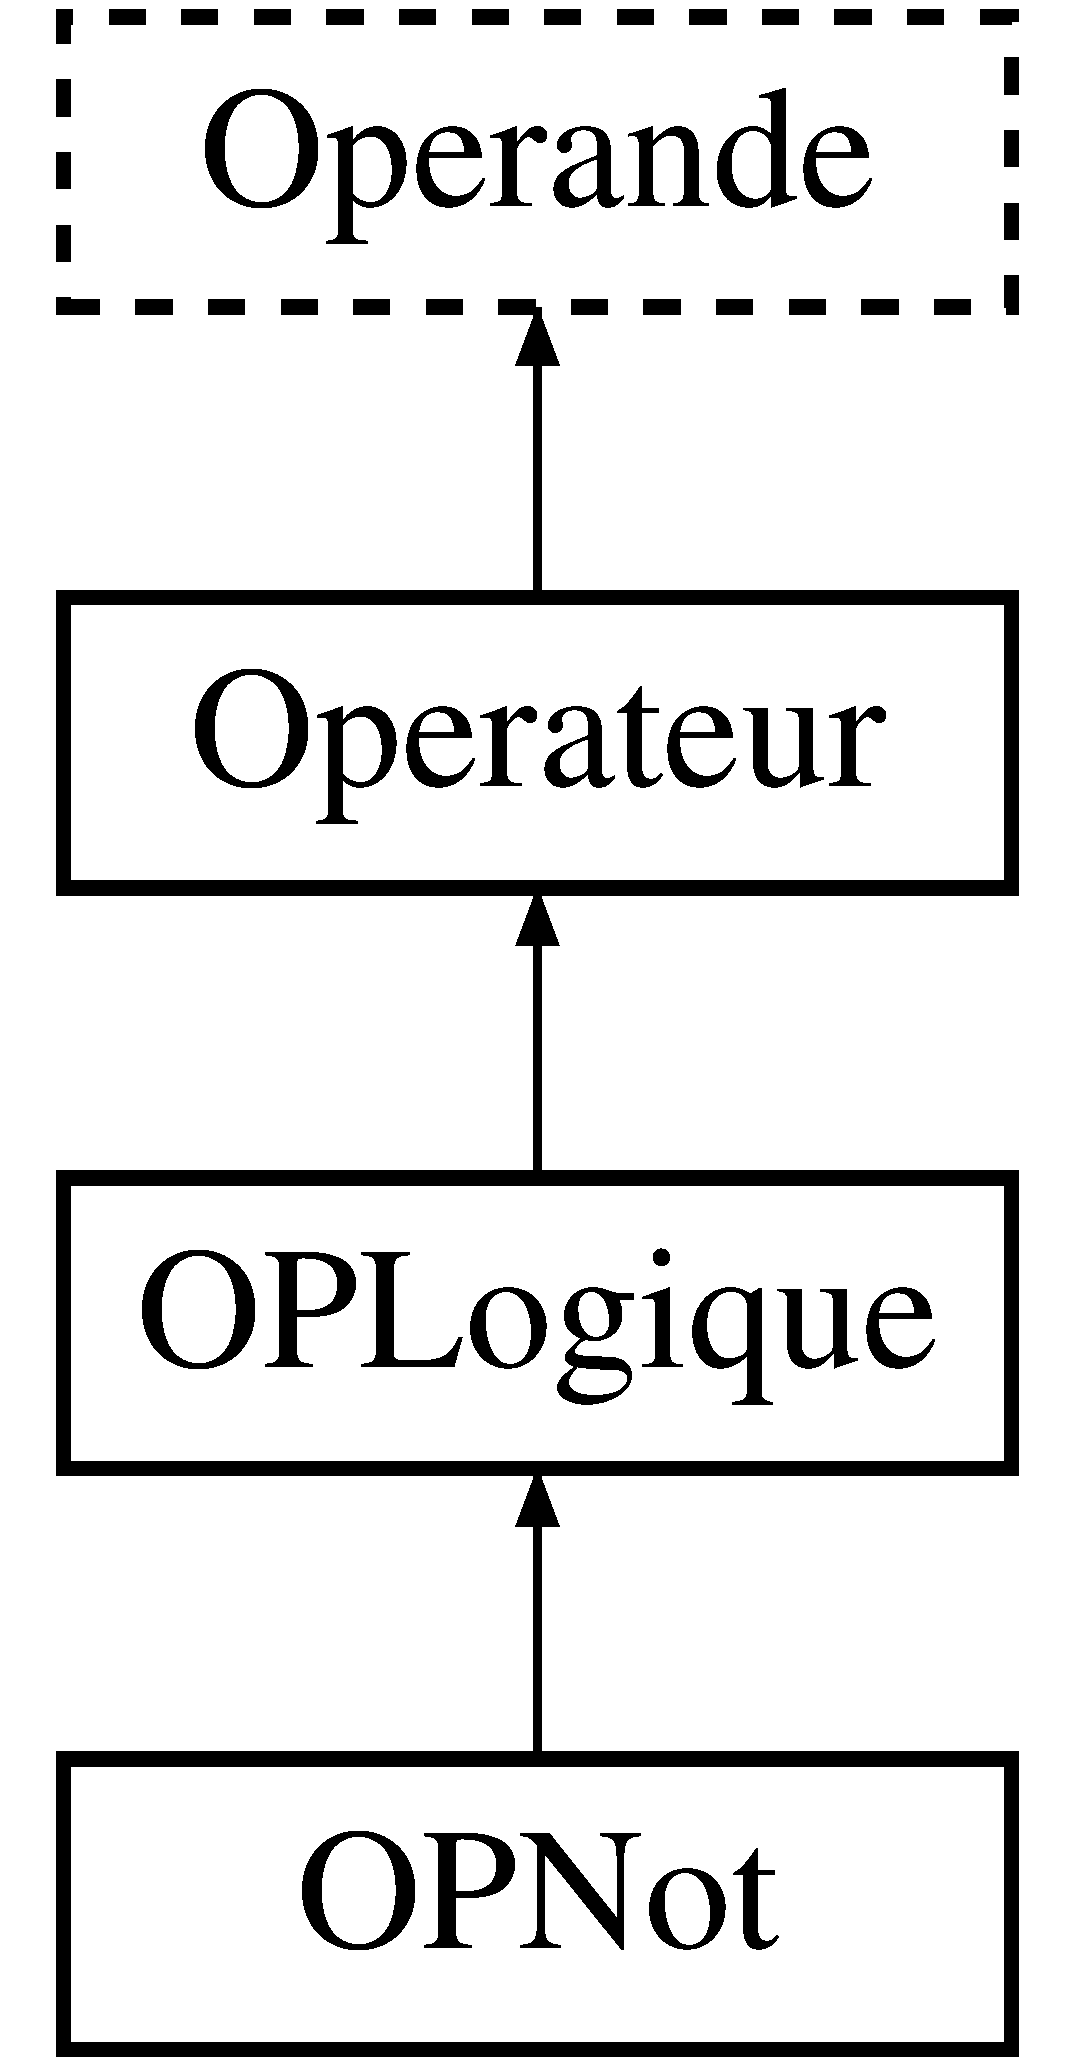
\includegraphics[height=4.000000cm]{class_o_p_not}
\end{center}
\end{figure}
\subsection*{Public Member Functions}
\begin{DoxyCompactItemize}
\item 
virtual \hyperlink{class_o_p_not}{O\+P\+Not} $\ast$ {\bfseries clone} () const \hypertarget{class_o_p_not_afb5934b18a041d14d96d40f16082e291}{}\label{class_o_p_not_afb5934b18a041d14d96d40f16082e291}

\item 
virtual \hyperlink{class_litterale}{Litterale} $\ast$ {\bfseries compute} ()\hypertarget{class_o_p_not_ac530d751ef848207c958a304f54af04c}{}\label{class_o_p_not_ac530d751ef848207c958a304f54af04c}

\item 
virtual \hyperlink{class_litterale}{Litterale} $\ast$ {\bfseries compute} (\hyperlink{class_litterale}{Litterale} $\ast$l)\hypertarget{class_o_p_not_a1e3513845f524579b14f8f9989e4c9fb}{}\label{class_o_p_not_a1e3513845f524579b14f8f9989e4c9fb}

\item 
virtual \hyperlink{class_litterale}{Litterale} $\ast$ {\bfseries compute} (\hyperlink{class_litterale}{Litterale} $\ast$l1, \hyperlink{class_litterale}{Litterale} $\ast$l2)\hypertarget{class_o_p_not_a11202c69a1cfce9e0bce813248e6e37b}{}\label{class_o_p_not_a11202c69a1cfce9e0bce813248e6e37b}

\end{DoxyCompactItemize}
\subsection*{Additional Inherited Members}


The documentation for this class was generated from the following files\+:\begin{DoxyCompactItemize}
\item 
oplogique.\+h\item 
oplogique.\+cpp\end{DoxyCompactItemize}

\hypertarget{class_o_p_num___l_t_sans_expression}{}\section{O\+P\+Num\+\_\+\+L\+T\+Sans\+Expression Class Reference}
\label{class_o_p_num___l_t_sans_expression}\index{O\+P\+Num\+\_\+\+L\+T\+Sans\+Expression@{O\+P\+Num\+\_\+\+L\+T\+Sans\+Expression}}
Inheritance diagram for O\+P\+Num\+\_\+\+L\+T\+Sans\+Expression\+:\begin{figure}[H]
\begin{center}
\leavevmode
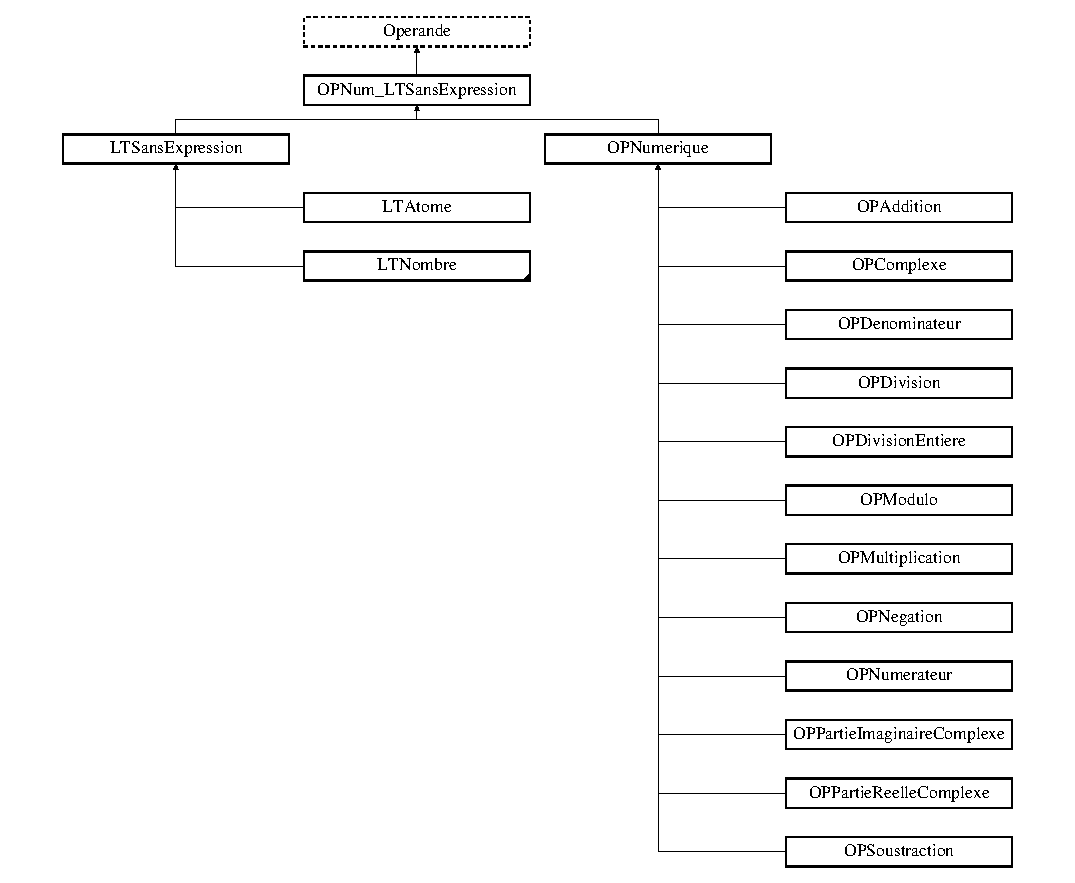
\includegraphics[height=11.413043cm]{class_o_p_num___l_t_sans_expression}
\end{center}
\end{figure}
\subsection*{Public Member Functions}
\begin{DoxyCompactItemize}
\item 
virtual \hyperlink{class_o_p_num___l_t_sans_expression}{O\+P\+Num\+\_\+\+L\+T\+Sans\+Expression} $\ast$ {\bfseries clone} () const  =0\hypertarget{class_o_p_num___l_t_sans_expression_a9f7c47913c9ca5d03f66a6918facd442}{}\label{class_o_p_num___l_t_sans_expression_a9f7c47913c9ca5d03f66a6918facd442}

\end{DoxyCompactItemize}


The documentation for this class was generated from the following files\+:\begin{DoxyCompactItemize}
\item 
opnum\+\_\+ltsansexpression.\+h\item 
opnum\+\_\+ltsansexpression.\+cpp\end{DoxyCompactItemize}

\hypertarget{class_o_p_numerateur}{}\section{O\+P\+Numerateur Class Reference}
\label{class_o_p_numerateur}\index{O\+P\+Numerateur@{O\+P\+Numerateur}}
Inheritance diagram for O\+P\+Numerateur\+:\begin{figure}[H]
\begin{center}
\leavevmode
\includegraphics[height=4.000000cm]{class_o_p_numerateur}
\end{center}
\end{figure}
\subsection*{Public Member Functions}
\begin{DoxyCompactItemize}
\item 
virtual \hyperlink{class_o_p_numerateur}{O\+P\+Numerateur} $\ast$ {\bfseries clone} () const \hypertarget{class_o_p_numerateur_a8cb830108d8967edece8eea14e6e736a}{}\label{class_o_p_numerateur_a8cb830108d8967edece8eea14e6e736a}

\item 
virtual \hyperlink{class_litterale}{Litterale} $\ast$ {\bfseries compute} ()\hypertarget{class_o_p_numerateur_a80c2db964bdceab04b37c64d0c1e64ad}{}\label{class_o_p_numerateur_a80c2db964bdceab04b37c64d0c1e64ad}

\item 
virtual \hyperlink{class_litterale}{Litterale} $\ast$ {\bfseries compute} (\hyperlink{class_litterale}{Litterale} $\ast$l)\hypertarget{class_o_p_numerateur_ad3e252d19ce88d5d4ac370fe8a578560}{}\label{class_o_p_numerateur_ad3e252d19ce88d5d4ac370fe8a578560}

\item 
virtual \hyperlink{class_litterale}{Litterale} $\ast$ {\bfseries compute} (\hyperlink{class_litterale}{Litterale} $\ast$l1, \hyperlink{class_litterale}{Litterale} $\ast$l2)\hypertarget{class_o_p_numerateur_ac94ae0e63f1736ddb63e35f07e84db6f}{}\label{class_o_p_numerateur_ac94ae0e63f1736ddb63e35f07e84db6f}

\end{DoxyCompactItemize}
\subsection*{Additional Inherited Members}


The documentation for this class was generated from the following files\+:\begin{DoxyCompactItemize}
\item 
opnumerique.\+h\item 
opnumerique.\+cpp\end{DoxyCompactItemize}

\hypertarget{class_o_p_numerique}{}\section{O\+P\+Numerique Class Reference}
\label{class_o_p_numerique}\index{O\+P\+Numerique@{O\+P\+Numerique}}
Inheritance diagram for O\+P\+Numerique\+:\begin{figure}[H]
\begin{center}
\leavevmode
\includegraphics[height=12.000000cm]{class_o_p_numerique}
\end{center}
\end{figure}
\subsection*{Public Member Functions}
\begin{DoxyCompactItemize}
\item 
{\bfseries O\+P\+Numerique} (Q\+String val, int a)\hypertarget{class_o_p_numerique_ae4edc185c642b986930dc3af3632100b}{}\label{class_o_p_numerique_ae4edc185c642b986930dc3af3632100b}

\item 
virtual \hyperlink{class_o_p_numerique}{O\+P\+Numerique} $\ast$ {\bfseries clone} () const  =0\hypertarget{class_o_p_numerique_a6cd9e71c2dcd91fc0116203918795575}{}\label{class_o_p_numerique_a6cd9e71c2dcd91fc0116203918795575}

\item 
virtual \hyperlink{class_litterale}{Litterale} $\ast$ {\bfseries compute} ()=0\hypertarget{class_o_p_numerique_a7ea5720f3721cf682912b17fd24f7505}{}\label{class_o_p_numerique_a7ea5720f3721cf682912b17fd24f7505}

\item 
virtual \hyperlink{class_litterale}{Litterale} $\ast$ {\bfseries compute} (\hyperlink{class_litterale}{Litterale} $\ast$l)=0\hypertarget{class_o_p_numerique_a38cf8b1a677cef5c9040b4f9a7351ade}{}\label{class_o_p_numerique_a38cf8b1a677cef5c9040b4f9a7351ade}

\item 
virtual \hyperlink{class_litterale}{Litterale} $\ast$ {\bfseries compute} (\hyperlink{class_litterale}{Litterale} $\ast$l1, \hyperlink{class_litterale}{Litterale} $\ast$l2)=0\hypertarget{class_o_p_numerique_a783635d833da49584cf5a7192a732284}{}\label{class_o_p_numerique_a783635d833da49584cf5a7192a732284}

\end{DoxyCompactItemize}
\subsection*{Additional Inherited Members}


The documentation for this class was generated from the following file\+:\begin{DoxyCompactItemize}
\item 
opnumerique.\+h\end{DoxyCompactItemize}

\hypertarget{class_o_p_or}{}\section{O\+P\+Or Class Reference}
\label{class_o_p_or}\index{O\+P\+Or@{O\+P\+Or}}
Inheritance diagram for O\+P\+Or\+:\begin{figure}[H]
\begin{center}
\leavevmode
\includegraphics[height=4.000000cm]{class_o_p_or}
\end{center}
\end{figure}
\subsection*{Public Member Functions}
\begin{DoxyCompactItemize}
\item 
virtual \hyperlink{class_o_p_or}{O\+P\+Or} $\ast$ {\bfseries clone} () const \hypertarget{class_o_p_or_a7d0187aebfddc4fe05b7ddae1bbceb08}{}\label{class_o_p_or_a7d0187aebfddc4fe05b7ddae1bbceb08}

\item 
virtual \hyperlink{class_litterale}{Litterale} $\ast$ {\bfseries compute} ()\hypertarget{class_o_p_or_af903164c338726e6d86d6f55300bdb08}{}\label{class_o_p_or_af903164c338726e6d86d6f55300bdb08}

\item 
virtual \hyperlink{class_litterale}{Litterale} $\ast$ {\bfseries compute} (\hyperlink{class_litterale}{Litterale} $\ast$l)\hypertarget{class_o_p_or_abbb1f72a37347f9dfaf66ecd38475905}{}\label{class_o_p_or_abbb1f72a37347f9dfaf66ecd38475905}

\item 
virtual \hyperlink{class_litterale}{Litterale} $\ast$ {\bfseries compute} (\hyperlink{class_litterale}{Litterale} $\ast$l1, \hyperlink{class_litterale}{Litterale} $\ast$l2)\hypertarget{class_o_p_or_a73ea1ffdfad3933a2a2af6f726a7ee6e}{}\label{class_o_p_or_a73ea1ffdfad3933a2a2af6f726a7ee6e}

\end{DoxyCompactItemize}
\subsection*{Additional Inherited Members}


The documentation for this class was generated from the following files\+:\begin{DoxyCompactItemize}
\item 
oplogique.\+h\item 
oplogique.\+cpp\end{DoxyCompactItemize}

\hypertarget{class_o_p_partie_imaginaire_complexe}{}\section{O\+P\+Partie\+Imaginaire\+Complexe Class Reference}
\label{class_o_p_partie_imaginaire_complexe}\index{O\+P\+Partie\+Imaginaire\+Complexe@{O\+P\+Partie\+Imaginaire\+Complexe}}
Inheritance diagram for O\+P\+Partie\+Imaginaire\+Complexe\+:\begin{figure}[H]
\begin{center}
\leavevmode
\includegraphics[height=4.000000cm]{class_o_p_partie_imaginaire_complexe}
\end{center}
\end{figure}
\subsection*{Public Member Functions}
\begin{DoxyCompactItemize}
\item 
virtual \hyperlink{class_o_p_partie_imaginaire_complexe}{O\+P\+Partie\+Imaginaire\+Complexe} $\ast$ {\bfseries clone} () const \hypertarget{class_o_p_partie_imaginaire_complexe_ae01d21bde49edb8106729a0c1b146fb0}{}\label{class_o_p_partie_imaginaire_complexe_ae01d21bde49edb8106729a0c1b146fb0}

\item 
virtual \hyperlink{class_litterale}{Litterale} $\ast$ {\bfseries compute} ()\hypertarget{class_o_p_partie_imaginaire_complexe_a60bcb1c7d4298e3bd8144fc1e7745865}{}\label{class_o_p_partie_imaginaire_complexe_a60bcb1c7d4298e3bd8144fc1e7745865}

\item 
virtual \hyperlink{class_litterale}{Litterale} $\ast$ {\bfseries compute} (\hyperlink{class_litterale}{Litterale} $\ast$l)\hypertarget{class_o_p_partie_imaginaire_complexe_a6de4292de1bfb10206f1d16f86f6a947}{}\label{class_o_p_partie_imaginaire_complexe_a6de4292de1bfb10206f1d16f86f6a947}

\item 
virtual \hyperlink{class_litterale}{Litterale} $\ast$ {\bfseries compute} (\hyperlink{class_litterale}{Litterale} $\ast$l1, \hyperlink{class_litterale}{Litterale} $\ast$l2)\hypertarget{class_o_p_partie_imaginaire_complexe_acce061b9fe7c9919ac76030638c44cc8}{}\label{class_o_p_partie_imaginaire_complexe_acce061b9fe7c9919ac76030638c44cc8}

\end{DoxyCompactItemize}
\subsection*{Additional Inherited Members}


The documentation for this class was generated from the following files\+:\begin{DoxyCompactItemize}
\item 
opnumerique.\+h\item 
opnumerique.\+cpp\end{DoxyCompactItemize}

\hypertarget{class_o_p_partie_reelle_complexe}{}\section{O\+P\+Partie\+Reelle\+Complexe Class Reference}
\label{class_o_p_partie_reelle_complexe}\index{O\+P\+Partie\+Reelle\+Complexe@{O\+P\+Partie\+Reelle\+Complexe}}
Inheritance diagram for O\+P\+Partie\+Reelle\+Complexe\+:\begin{figure}[H]
\begin{center}
\leavevmode
\includegraphics[height=4.000000cm]{class_o_p_partie_reelle_complexe}
\end{center}
\end{figure}
\subsection*{Public Member Functions}
\begin{DoxyCompactItemize}
\item 
virtual \hyperlink{class_o_p_partie_reelle_complexe}{O\+P\+Partie\+Reelle\+Complexe} $\ast$ {\bfseries clone} () const \hypertarget{class_o_p_partie_reelle_complexe_ab0b419202cefa7f4bd0940faafb15e1b}{}\label{class_o_p_partie_reelle_complexe_ab0b419202cefa7f4bd0940faafb15e1b}

\item 
virtual \hyperlink{class_litterale}{Litterale} $\ast$ {\bfseries compute} ()\hypertarget{class_o_p_partie_reelle_complexe_a1ef3a295a6b3b6aa1474f62d128b8239}{}\label{class_o_p_partie_reelle_complexe_a1ef3a295a6b3b6aa1474f62d128b8239}

\item 
virtual \hyperlink{class_litterale}{Litterale} $\ast$ {\bfseries compute} (\hyperlink{class_litterale}{Litterale} $\ast$l)\hypertarget{class_o_p_partie_reelle_complexe_a39c7ccd465c93592ef49d9695081efbd}{}\label{class_o_p_partie_reelle_complexe_a39c7ccd465c93592ef49d9695081efbd}

\item 
virtual \hyperlink{class_litterale}{Litterale} $\ast$ {\bfseries compute} (\hyperlink{class_litterale}{Litterale} $\ast$l1, \hyperlink{class_litterale}{Litterale} $\ast$l2)\hypertarget{class_o_p_partie_reelle_complexe_ab43515992604e136042404626cea2dcb}{}\label{class_o_p_partie_reelle_complexe_ab43515992604e136042404626cea2dcb}

\end{DoxyCompactItemize}
\subsection*{Additional Inherited Members}


The documentation for this class was generated from the following files\+:\begin{DoxyCompactItemize}
\item 
opnumerique.\+h\item 
opnumerique.\+cpp\end{DoxyCompactItemize}

\hypertarget{class_o_p_redo}{}\section{O\+P\+Redo Class Reference}
\label{class_o_p_redo}\index{O\+P\+Redo@{O\+P\+Redo}}
Inheritance diagram for O\+P\+Redo\+:\begin{figure}[H]
\begin{center}
\leavevmode
\includegraphics[height=4.000000cm]{class_o_p_redo}
\end{center}
\end{figure}
\subsection*{Public Member Functions}
\begin{DoxyCompactItemize}
\item 
virtual \hyperlink{class_o_p_redo}{O\+P\+Redo} $\ast$ {\bfseries clone} () const \hypertarget{class_o_p_redo_afcbce83d13bac98e74661980ce5f4e34}{}\label{class_o_p_redo_afcbce83d13bac98e74661980ce5f4e34}

\item 
virtual \hyperlink{class_litterale}{Litterale} $\ast$ {\bfseries compute} ()\hypertarget{class_o_p_redo_aa794c07a788d5a23d37914f713d2939d}{}\label{class_o_p_redo_aa794c07a788d5a23d37914f713d2939d}

\item 
virtual \hyperlink{class_litterale}{Litterale} $\ast$ {\bfseries compute} (\hyperlink{class_litterale}{Litterale} $\ast$l)\hypertarget{class_o_p_redo_ae971828a6ae3ba538461bba6ebb00974}{}\label{class_o_p_redo_ae971828a6ae3ba538461bba6ebb00974}

\item 
virtual \hyperlink{class_litterale}{Litterale} $\ast$ {\bfseries compute} (\hyperlink{class_litterale}{Litterale} $\ast$l1, \hyperlink{class_litterale}{Litterale} $\ast$l2)\hypertarget{class_o_p_redo_afebdb64e5647f024961dbbae578d96cb}{}\label{class_o_p_redo_afebdb64e5647f024961dbbae578d96cb}

\end{DoxyCompactItemize}
\subsection*{Additional Inherited Members}


The documentation for this class was generated from the following files\+:\begin{DoxyCompactItemize}
\item 
opmanipulationpile.\+h\item 
opmanipulationpile.\+cpp\end{DoxyCompactItemize}

\hypertarget{class_o_p_soustraction}{}\section{O\+P\+Soustraction Class Reference}
\label{class_o_p_soustraction}\index{O\+P\+Soustraction@{O\+P\+Soustraction}}
Inheritance diagram for O\+P\+Soustraction\+:\begin{figure}[H]
\begin{center}
\leavevmode
\includegraphics[height=4.000000cm]{class_o_p_soustraction}
\end{center}
\end{figure}
\subsection*{Public Member Functions}
\begin{DoxyCompactItemize}
\item 
virtual \hyperlink{class_o_p_soustraction}{O\+P\+Soustraction} $\ast$ {\bfseries clone} () const \hypertarget{class_o_p_soustraction_a4e7ca9166e50f0c281eea55db792244a}{}\label{class_o_p_soustraction_a4e7ca9166e50f0c281eea55db792244a}

\item 
virtual \hyperlink{class_litterale}{Litterale} $\ast$ {\bfseries compute} ()\hypertarget{class_o_p_soustraction_a6926b8b60c9bb6bcaf91ef042f347dc3}{}\label{class_o_p_soustraction_a6926b8b60c9bb6bcaf91ef042f347dc3}

\item 
virtual \hyperlink{class_litterale}{Litterale} $\ast$ {\bfseries compute} (\hyperlink{class_litterale}{Litterale} $\ast$l)\hypertarget{class_o_p_soustraction_a9ac5ca3bd73414d5e3033e9d63ad7740}{}\label{class_o_p_soustraction_a9ac5ca3bd73414d5e3033e9d63ad7740}

\item 
virtual \hyperlink{class_litterale}{Litterale} $\ast$ {\bfseries compute} (\hyperlink{class_litterale}{Litterale} $\ast$l1, \hyperlink{class_litterale}{Litterale} $\ast$l2)\hypertarget{class_o_p_soustraction_af4ef17eac91bbf0f41475479e9817179}{}\label{class_o_p_soustraction_af4ef17eac91bbf0f41475479e9817179}

\end{DoxyCompactItemize}
\subsection*{Additional Inherited Members}


The documentation for this class was generated from the following files\+:\begin{DoxyCompactItemize}
\item 
opnumerique.\+h\item 
opnumerique.\+cpp\end{DoxyCompactItemize}

\hypertarget{class_o_p_sto}{}\section{O\+P\+Sto Class Reference}
\label{class_o_p_sto}\index{O\+P\+Sto@{O\+P\+Sto}}
Inheritance diagram for O\+P\+Sto\+:\begin{figure}[H]
\begin{center}
\leavevmode
\includegraphics[height=4.000000cm]{class_o_p_sto}
\end{center}
\end{figure}
\subsection*{Public Member Functions}
\begin{DoxyCompactItemize}
\item 
virtual \hyperlink{class_o_p_sto}{O\+P\+Sto} $\ast$ {\bfseries clone} () const \hypertarget{class_o_p_sto_af06eca95a7efdb74a9e63491da02067f}{}\label{class_o_p_sto_af06eca95a7efdb74a9e63491da02067f}

\item 
virtual \hyperlink{class_litterale}{Litterale} $\ast$ {\bfseries compute} ()\hypertarget{class_o_p_sto_a1334907b87e8626bc830210fd13b959a}{}\label{class_o_p_sto_a1334907b87e8626bc830210fd13b959a}

\item 
virtual \hyperlink{class_litterale}{Litterale} $\ast$ {\bfseries compute} (\hyperlink{class_litterale}{Litterale} $\ast$l)\hypertarget{class_o_p_sto_aebe8dc34d4a4f3cd7a434a4e2314b5ef}{}\label{class_o_p_sto_aebe8dc34d4a4f3cd7a434a4e2314b5ef}

\item 
virtual \hyperlink{class_litterale}{Litterale} $\ast$ {\bfseries compute} (\hyperlink{class_litterale}{Litterale} $\ast$l1, \hyperlink{class_litterale}{Litterale} $\ast$l2)\hypertarget{class_o_p_sto_a28753ee9a6e433f477ec3197feccafdd}{}\label{class_o_p_sto_a28753ee9a6e433f477ec3197feccafdd}

\end{DoxyCompactItemize}
\subsection*{Additional Inherited Members}


The documentation for this class was generated from the following files\+:\begin{DoxyCompactItemize}
\item 
opatome.\+h\item 
opatome.\+cpp\end{DoxyCompactItemize}

\hypertarget{class_o_p_superieur}{}\section{O\+P\+Superieur Class Reference}
\label{class_o_p_superieur}\index{O\+P\+Superieur@{O\+P\+Superieur}}
Inheritance diagram for O\+P\+Superieur\+:\begin{figure}[H]
\begin{center}
\leavevmode
\includegraphics[height=4.000000cm]{class_o_p_superieur}
\end{center}
\end{figure}
\subsection*{Public Member Functions}
\begin{DoxyCompactItemize}
\item 
virtual \hyperlink{class_o_p_superieur}{O\+P\+Superieur} $\ast$ {\bfseries clone} () const \hypertarget{class_o_p_superieur_ab923304921d13d5840e7c22ef5527c0a}{}\label{class_o_p_superieur_ab923304921d13d5840e7c22ef5527c0a}

\item 
virtual \hyperlink{class_litterale}{Litterale} $\ast$ {\bfseries compute} ()\hypertarget{class_o_p_superieur_a611ce07b54744c2d1ca6b6f9d56de628}{}\label{class_o_p_superieur_a611ce07b54744c2d1ca6b6f9d56de628}

\item 
virtual \hyperlink{class_litterale}{Litterale} $\ast$ {\bfseries compute} (\hyperlink{class_litterale}{Litterale} $\ast$l)\hypertarget{class_o_p_superieur_aee73e7270974181b5d5ec2ec4cd16491}{}\label{class_o_p_superieur_aee73e7270974181b5d5ec2ec4cd16491}

\item 
virtual \hyperlink{class_litterale}{Litterale} $\ast$ {\bfseries compute} (\hyperlink{class_litterale}{Litterale} $\ast$l1, \hyperlink{class_litterale}{Litterale} $\ast$l2)\hypertarget{class_o_p_superieur_a2bd7a4323e745139cf60bf0c5faf2437}{}\label{class_o_p_superieur_a2bd7a4323e745139cf60bf0c5faf2437}

\end{DoxyCompactItemize}
\subsection*{Additional Inherited Members}


The documentation for this class was generated from the following files\+:\begin{DoxyCompactItemize}
\item 
oplogique.\+h\item 
oplogique.\+cpp\end{DoxyCompactItemize}

\hypertarget{class_o_p_superieur_egal}{}\section{O\+P\+Superieur\+Egal Class Reference}
\label{class_o_p_superieur_egal}\index{O\+P\+Superieur\+Egal@{O\+P\+Superieur\+Egal}}
Inheritance diagram for O\+P\+Superieur\+Egal\+:\begin{figure}[H]
\begin{center}
\leavevmode
\includegraphics[height=4.000000cm]{class_o_p_superieur_egal}
\end{center}
\end{figure}
\subsection*{Public Member Functions}
\begin{DoxyCompactItemize}
\item 
virtual \hyperlink{class_o_p_superieur_egal}{O\+P\+Superieur\+Egal} $\ast$ {\bfseries clone} () const \hypertarget{class_o_p_superieur_egal_a676bc0c7dcce000f16d0277284345642}{}\label{class_o_p_superieur_egal_a676bc0c7dcce000f16d0277284345642}

\item 
virtual \hyperlink{class_litterale}{Litterale} $\ast$ {\bfseries compute} ()\hypertarget{class_o_p_superieur_egal_a0d47eca022c03018d035b965f50f0dd5}{}\label{class_o_p_superieur_egal_a0d47eca022c03018d035b965f50f0dd5}

\item 
virtual \hyperlink{class_litterale}{Litterale} $\ast$ {\bfseries compute} (\hyperlink{class_litterale}{Litterale} $\ast$l)\hypertarget{class_o_p_superieur_egal_a8f54937140dc99025ff96824f6a3a41c}{}\label{class_o_p_superieur_egal_a8f54937140dc99025ff96824f6a3a41c}

\item 
virtual \hyperlink{class_litterale}{Litterale} $\ast$ {\bfseries compute} (\hyperlink{class_litterale}{Litterale} $\ast$l1, \hyperlink{class_litterale}{Litterale} $\ast$l2)\hypertarget{class_o_p_superieur_egal_aedb75bbbf56e3e3b9dbe81c7cba71a30}{}\label{class_o_p_superieur_egal_aedb75bbbf56e3e3b9dbe81c7cba71a30}

\end{DoxyCompactItemize}
\subsection*{Additional Inherited Members}


The documentation for this class was generated from the following files\+:\begin{DoxyCompactItemize}
\item 
oplogique.\+h\item 
oplogique.\+cpp\end{DoxyCompactItemize}

\hypertarget{class_o_p_swap}{}\section{O\+P\+Swap Class Reference}
\label{class_o_p_swap}\index{O\+P\+Swap@{O\+P\+Swap}}
Inheritance diagram for O\+P\+Swap\+:\begin{figure}[H]
\begin{center}
\leavevmode
\includegraphics[height=4.000000cm]{class_o_p_swap}
\end{center}
\end{figure}
\subsection*{Public Member Functions}
\begin{DoxyCompactItemize}
\item 
virtual \hyperlink{class_o_p_swap}{O\+P\+Swap} $\ast$ {\bfseries clone} () const \hypertarget{class_o_p_swap_a6ec92b4e33b2cdeef35e04e22e48e433}{}\label{class_o_p_swap_a6ec92b4e33b2cdeef35e04e22e48e433}

\item 
virtual \hyperlink{class_litterale}{Litterale} $\ast$ {\bfseries compute} ()\hypertarget{class_o_p_swap_aab3a06a4ddefe008a5fa771efea2b41c}{}\label{class_o_p_swap_aab3a06a4ddefe008a5fa771efea2b41c}

\item 
virtual \hyperlink{class_litterale}{Litterale} $\ast$ {\bfseries compute} (\hyperlink{class_litterale}{Litterale} $\ast$l)\hypertarget{class_o_p_swap_a0d3ddab48fcd270c4df00a22e2d5cd6f}{}\label{class_o_p_swap_a0d3ddab48fcd270c4df00a22e2d5cd6f}

\item 
virtual \hyperlink{class_litterale}{Litterale} $\ast$ {\bfseries compute} (\hyperlink{class_litterale}{Litterale} $\ast$l1, \hyperlink{class_litterale}{Litterale} $\ast$l2)\hypertarget{class_o_p_swap_a1ca0b42e1bc12addd98b2640ce5f93b7}{}\label{class_o_p_swap_a1ca0b42e1bc12addd98b2640ce5f93b7}

\end{DoxyCompactItemize}
\subsection*{Additional Inherited Members}


The documentation for this class was generated from the following files\+:\begin{DoxyCompactItemize}
\item 
opmanipulationpile.\+h\item 
opmanipulationpile.\+cpp\end{DoxyCompactItemize}

\hypertarget{class_o_p_undo}{}\section{O\+P\+Undo Class Reference}
\label{class_o_p_undo}\index{O\+P\+Undo@{O\+P\+Undo}}
Inheritance diagram for O\+P\+Undo\+:\begin{figure}[H]
\begin{center}
\leavevmode
\includegraphics[height=4.000000cm]{class_o_p_undo}
\end{center}
\end{figure}
\subsection*{Public Member Functions}
\begin{DoxyCompactItemize}
\item 
virtual \hyperlink{class_o_p_undo}{O\+P\+Undo} $\ast$ {\bfseries clone} () const \hypertarget{class_o_p_undo_a35a6a21c99215de99771a61710f5b346}{}\label{class_o_p_undo_a35a6a21c99215de99771a61710f5b346}

\item 
virtual \hyperlink{class_litterale}{Litterale} $\ast$ {\bfseries compute} ()\hypertarget{class_o_p_undo_a99ade45ce5516de33e4a1e89627a95ef}{}\label{class_o_p_undo_a99ade45ce5516de33e4a1e89627a95ef}

\item 
virtual \hyperlink{class_litterale}{Litterale} $\ast$ {\bfseries compute} (\hyperlink{class_litterale}{Litterale} $\ast$l)\hypertarget{class_o_p_undo_a7cd5dd4bba9c037e267af70ef63ae746}{}\label{class_o_p_undo_a7cd5dd4bba9c037e267af70ef63ae746}

\item 
virtual \hyperlink{class_litterale}{Litterale} $\ast$ {\bfseries compute} (\hyperlink{class_litterale}{Litterale} $\ast$l1, \hyperlink{class_litterale}{Litterale} $\ast$l2)\hypertarget{class_o_p_undo_af1c2d82c99ff4572243a431f8a3524b9}{}\label{class_o_p_undo_af1c2d82c99ff4572243a431f8a3524b9}

\end{DoxyCompactItemize}
\subsection*{Additional Inherited Members}


The documentation for this class was generated from the following files\+:\begin{DoxyCompactItemize}
\item 
opmanipulationpile.\+h\item 
opmanipulationpile.\+cpp\end{DoxyCompactItemize}

\hypertarget{class_originator}{}\section{Originator Class Reference}
\label{class_originator}\index{Originator@{Originator}}
\subsection*{Public Member Functions}
\begin{DoxyCompactItemize}
\item 
void {\bfseries set\+Stack} (\hyperlink{class_stack}{Stack} $\ast$s)\hypertarget{class_originator_a2ec52c4bc4d9e2112ed69add7bfe4024}{}\label{class_originator_a2ec52c4bc4d9e2112ed69add7bfe4024}

\item 
\hyperlink{class_memento}{Memento} {\bfseries store\+In\+Memento} ()\hypertarget{class_originator_a8a13e62dc073a01209075f117c0c4ff0}{}\label{class_originator_a8a13e62dc073a01209075f117c0c4ff0}

\item 
\hyperlink{class_stack}{Stack} $\ast$ {\bfseries restore\+From\+Memento} (\hyperlink{class_memento}{Memento} m)\hypertarget{class_originator_a180058583fd3a64798d0066ab360c3c6}{}\label{class_originator_a180058583fd3a64798d0066ab360c3c6}

\end{DoxyCompactItemize}


The documentation for this class was generated from the following file\+:\begin{DoxyCompactItemize}
\item 
memento.\+h\end{DoxyCompactItemize}

\hypertarget{class_parseur}{}\section{Parseur Class Reference}
\label{class_parseur}\index{Parseur@{Parseur}}
\subsection*{Static Public Member Functions}
\begin{DoxyCompactItemize}
\item 
static Q\+List$<$ \hyperlink{class_operande}{Operande} $\ast$ $>$ {\bfseries New\+List\+Operande} (const Q\+String \&chaine)\hypertarget{class_parseur_ad4ccbd4c6a37c367831ab6388c0802bc}{}\label{class_parseur_ad4ccbd4c6a37c367831ab6388c0802bc}

\item 
static Q\+List$<$ \hyperlink{class_o_p_num___l_t_sans_expression}{O\+P\+Num\+\_\+\+L\+T\+Sans\+Expression} $\ast$ $>$ {\bfseries New\+List\+O\+P\+Num\+\_\+\+L\+T\+Sans\+Expression} (const Q\+String \&chaine)\hypertarget{class_parseur_aa8fd6265a08f5bec6f2a90fed7fd0416}{}\label{class_parseur_aa8fd6265a08f5bec6f2a90fed7fd0416}

\end{DoxyCompactItemize}


The documentation for this class was generated from the following files\+:\begin{DoxyCompactItemize}
\item 
parseur.\+h\item 
parseur.\+cpp\end{DoxyCompactItemize}

\hypertarget{class_stack}{}\section{Stack Class Reference}
\label{class_stack}\index{Stack@{Stack}}
\subsection*{Public Member Functions}
\begin{DoxyCompactItemize}
\item 
void {\bfseries swap} (Q\+List$<$ \hyperlink{class_litterale}{Litterale} $\ast$ $>$ \&other)\hypertarget{class_stack_a906e42093ef691a5a2225f4787e6218e}{}\label{class_stack_a906e42093ef691a5a2225f4787e6218e}

\item 
void {\bfseries push} (\hyperlink{class_litterale}{Litterale} $\ast$t)\hypertarget{class_stack_a4ff65039d5bf329702f5d30a9c9689e7}{}\label{class_stack_a4ff65039d5bf329702f5d30a9c9689e7}

\item 
\hyperlink{class_litterale}{Litterale} $\ast$ {\bfseries pop} ()  throw (\+Exception\+Stack)\hypertarget{class_stack_a37e9667dbeef8cb79d9cb4bdbaebb72b}{}\label{class_stack_a37e9667dbeef8cb79d9cb4bdbaebb72b}

\item 
bool {\bfseries can\+Pop\+Items} (unsigned int nb) const \hypertarget{class_stack_a171d983f57d41db07825233864a78447}{}\label{class_stack_a171d983f57d41db07825233864a78447}

\item 
bool {\bfseries is\+Empty} () const \hypertarget{class_stack_a5dea07bd80438c88ea0bcd5db50a8cec}{}\label{class_stack_a5dea07bd80438c88ea0bcd5db50a8cec}

\item 
void {\bfseries clear} ()\hypertarget{class_stack_adab1284b8929385d4020356fb52c8139}{}\label{class_stack_adab1284b8929385d4020356fb52c8139}

\item 
const \hyperlink{class_litterale}{Litterale} $\ast$ {\bfseries operator\mbox{[}$\,$\mbox{]}} (unsigned int index) const \hypertarget{class_stack_aef76f74d885d102151cc4e2cb236bcca}{}\label{class_stack_aef76f74d885d102151cc4e2cb236bcca}

\item 
unsigned int {\bfseries size} () const \hypertarget{class_stack_a099ad429ca3504cda12946897ab1cf15}{}\label{class_stack_a099ad429ca3504cda12946897ab1cf15}

\item 
\hyperlink{class_stack}{Stack} $\ast$ {\bfseries clone} () const \hypertarget{class_stack_aa2f1d52b0d1dc07b45bcda4894067742}{}\label{class_stack_aa2f1d52b0d1dc07b45bcda4894067742}

\item 
Q\+List$<$ \hyperlink{class_litterale}{Litterale} $\ast$ $>$ {\bfseries get\+Stack\+Items} () const \hypertarget{class_stack_ae6d2e7608f796cafbe36ee4e54895654}{}\label{class_stack_ae6d2e7608f796cafbe36ee4e54895654}

\end{DoxyCompactItemize}


The documentation for this class was generated from the following file\+:\begin{DoxyCompactItemize}
\item 
stack.\+h\end{DoxyCompactItemize}

\hypertarget{class_u_i_button}{}\section{U\+I\+Button Class Reference}
\label{class_u_i_button}\index{U\+I\+Button@{U\+I\+Button}}
Inheritance diagram for U\+I\+Button\+:\begin{figure}[H]
\begin{center}
\leavevmode
\includegraphics[height=2.000000cm]{class_u_i_button}
\end{center}
\end{figure}
\subsection*{Public Slots}
\begin{DoxyCompactItemize}
\item 
void {\bfseries has\+Been\+Clicked} ()\hypertarget{class_u_i_button_ad26644e8110959776eb35d4344dc9643}{}\label{class_u_i_button_ad26644e8110959776eb35d4344dc9643}

\end{DoxyCompactItemize}
\subsection*{Public Member Functions}
\begin{DoxyCompactItemize}
\item 
{\bfseries U\+I\+Button} (Q\+String text, float width=1, Q\+String v=\char`\"{}\char`\"{})\hypertarget{class_u_i_button_ac9d769d4b51156313eee17f18e4cee49}{}\label{class_u_i_button_ac9d769d4b51156313eee17f18e4cee49}

\item 
Q\+String {\bfseries get\+Value} () const \hypertarget{class_u_i_button_a86f2e2f571013d90f302ea615dd050bf}{}\label{class_u_i_button_a86f2e2f571013d90f302ea615dd050bf}

\end{DoxyCompactItemize}


The documentation for this class was generated from the following files\+:\begin{DoxyCompactItemize}
\item 
uibutton.\+h\item 
uibutton.\+cpp\end{DoxyCompactItemize}

\hypertarget{class_u_i_buttons_line}{}\section{U\+I\+Buttons\+Line Class Reference}
\label{class_u_i_buttons_line}\index{U\+I\+Buttons\+Line@{U\+I\+Buttons\+Line}}
Inheritance diagram for U\+I\+Buttons\+Line\+:\begin{figure}[H]
\begin{center}
\leavevmode
\includegraphics[height=2.000000cm]{class_u_i_buttons_line}
\end{center}
\end{figure}
\subsection*{Public Member Functions}
\begin{DoxyCompactItemize}
\item 
{\bfseries U\+I\+Buttons\+Line} (Q\+Widget $\ast$wdg=0)\hypertarget{class_u_i_buttons_line_a53d30e19ee72124286ec9b6a2d6e15f0}{}\label{class_u_i_buttons_line_a53d30e19ee72124286ec9b6a2d6e15f0}

\item 
void {\bfseries add\+Button} (\hyperlink{class_u_i_button}{U\+I\+Button} $\ast$btn)\hypertarget{class_u_i_buttons_line_a464c6748e2a71bd7bc5af566ba934ac0}{}\label{class_u_i_buttons_line_a464c6748e2a71bd7bc5af566ba934ac0}

\item 
void {\bfseries add\+Space} ()\hypertarget{class_u_i_buttons_line_a273a60c36299815ce2dd280471f881a1}{}\label{class_u_i_buttons_line_a273a60c36299815ce2dd280471f881a1}

\end{DoxyCompactItemize}


The documentation for this class was generated from the following file\+:\begin{DoxyCompactItemize}
\item 
uibuttonsline.\+h\end{DoxyCompactItemize}

\hypertarget{class_u_i_command_line}{}\section{U\+I\+Command\+Line Class Reference}
\label{class_u_i_command_line}\index{U\+I\+Command\+Line@{U\+I\+Command\+Line}}
Inheritance diagram for U\+I\+Command\+Line\+:\begin{figure}[H]
\begin{center}
\leavevmode
\includegraphics[height=2.000000cm]{class_u_i_command_line}
\end{center}
\end{figure}
\subsection*{Public Member Functions}
\begin{DoxyCompactItemize}
\item 
void {\bfseries write} (const Q\+String text)\hypertarget{class_u_i_command_line_af6c0336c21b3b3a6a2b3b9970759fa88}{}\label{class_u_i_command_line_af6c0336c21b3b3a6a2b3b9970759fa88}

\item 
void {\bfseries delete\+Last\+Character} ()\hypertarget{class_u_i_command_line_ac3fd2096fa3e15952e0fafd4c932ca9b}{}\label{class_u_i_command_line_ac3fd2096fa3e15952e0fafd4c932ca9b}

\item 
void {\bfseries clear} ()\hypertarget{class_u_i_command_line_af9b2dc89dd92b99f13c2afed6ec9f352}{}\label{class_u_i_command_line_af9b2dc89dd92b99f13c2afed6ec9f352}

\end{DoxyCompactItemize}


The documentation for this class was generated from the following file\+:\begin{DoxyCompactItemize}
\item 
uicommandeline.\+h\end{DoxyCompactItemize}

\hypertarget{class_u_i_create_var_window}{}\section{U\+I\+Create\+Var\+Window Class Reference}
\label{class_u_i_create_var_window}\index{U\+I\+Create\+Var\+Window@{U\+I\+Create\+Var\+Window}}
Inheritance diagram for U\+I\+Create\+Var\+Window\+:\begin{figure}[H]
\begin{center}
\leavevmode
\includegraphics[height=2.000000cm]{class_u_i_create_var_window}
\end{center}
\end{figure}
\subsection*{Public Slots}
\begin{DoxyCompactItemize}
\item 
void {\bfseries save\+Change} ()\hypertarget{class_u_i_create_var_window_af32556e9bd60360594f980f868fbcf71}{}\label{class_u_i_create_var_window_af32556e9bd60360594f980f868fbcf71}

\item 
void {\bfseries close\+Window} ()\hypertarget{class_u_i_create_var_window_acfc107eff898d9fa1d3b256591667d31}{}\label{class_u_i_create_var_window_acfc107eff898d9fa1d3b256591667d31}

\end{DoxyCompactItemize}
\subsection*{Public Member Functions}
\begin{DoxyCompactItemize}
\item 
void {\bfseries set\+Var\+Name} (Q\+String \&t)\hypertarget{class_u_i_create_var_window_a5f11db2930e89e733acace6a05b969d6}{}\label{class_u_i_create_var_window_a5f11db2930e89e733acace6a05b969d6}

\item 
void {\bfseries set\+Var\+Content} (Q\+String \&t)\hypertarget{class_u_i_create_var_window_ab6ee7f49fdad1be69d945dd8e3358294}{}\label{class_u_i_create_var_window_ab6ee7f49fdad1be69d945dd8e3358294}

\item 
void {\bfseries reload\+And\+Show} (Q\+String type)\hypertarget{class_u_i_create_var_window_af04acdd098c4ac941684a4318aefbb0e}{}\label{class_u_i_create_var_window_af04acdd098c4ac941684a4318aefbb0e}

\item 
void {\bfseries reload\+And\+Show} (Q\+String name, Q\+String content, Q\+String type)\hypertarget{class_u_i_create_var_window_a0909f33858c4377f2fdbc9b7cf46aed9}{}\label{class_u_i_create_var_window_a0909f33858c4377f2fdbc9b7cf46aed9}

\end{DoxyCompactItemize}
\subsection*{Static Public Member Functions}
\begin{DoxyCompactItemize}
\item 
static \hyperlink{class_u_i_create_var_window}{U\+I\+Create\+Var\+Window} \& {\bfseries get\+Instance} (Q\+Widget $\ast$parent=0, Q\+String name=\char`\"{}\char`\"{}, Q\+String content=\char`\"{}\char`\"{}, Q\+String type=\char`\"{}\char`\"{})\hypertarget{class_u_i_create_var_window_a8d341769adf8848860b2c850f9b3a90f}{}\label{class_u_i_create_var_window_a8d341769adf8848860b2c850f9b3a90f}

\item 
static void {\bfseries free\+Instance} ()\hypertarget{class_u_i_create_var_window_a7c62f9117201ac440bb9ee8803bf96a6}{}\label{class_u_i_create_var_window_a7c62f9117201ac440bb9ee8803bf96a6}

\end{DoxyCompactItemize}


The documentation for this class was generated from the following files\+:\begin{DoxyCompactItemize}
\item 
uicreatevarwindow.\+h\item 
uicreatevarwindow.\+cpp\end{DoxyCompactItemize}

\hypertarget{class_u_i_keyboard}{}\section{U\+I\+Keyboard Class Reference}
\label{class_u_i_keyboard}\index{U\+I\+Keyboard@{U\+I\+Keyboard}}
Inheritance diagram for U\+I\+Keyboard\+:\begin{figure}[H]
\begin{center}
\leavevmode
\includegraphics[height=2.000000cm]{class_u_i_keyboard}
\end{center}
\end{figure}
\subsection*{Public Member Functions}
\begin{DoxyCompactItemize}
\item 
{\bfseries U\+I\+Keyboard} (Q\+Widget $\ast$parent=0)\hypertarget{class_u_i_keyboard_a11dfa6dd929e8862b228efbce75cef4d}{}\label{class_u_i_keyboard_a11dfa6dd929e8862b228efbce75cef4d}

\item 
void {\bfseries init\+Keyboard} ()\hypertarget{class_u_i_keyboard_a7abefb6ff0d36a3c7422bfea10def61a}{}\label{class_u_i_keyboard_a7abefb6ff0d36a3c7422bfea10def61a}

\end{DoxyCompactItemize}
\subsection*{Public Attributes}
\begin{DoxyCompactItemize}
\item 
\hyperlink{class_u_i_keyboard_layout}{U\+I\+Keyboard\+Layout} $\ast$ {\bfseries layout}\hypertarget{class_u_i_keyboard_a869e22e5d5af43d5e2f4afabbb3f5953}{}\label{class_u_i_keyboard_a869e22e5d5af43d5e2f4afabbb3f5953}

\end{DoxyCompactItemize}


The documentation for this class was generated from the following file\+:\begin{DoxyCompactItemize}
\item 
uiclavier.\+h\end{DoxyCompactItemize}

\hypertarget{class_u_i_keyboard_layout}{}\section{U\+I\+Keyboard\+Layout Class Reference}
\label{class_u_i_keyboard_layout}\index{U\+I\+Keyboard\+Layout@{U\+I\+Keyboard\+Layout}}
Inheritance diagram for U\+I\+Keyboard\+Layout\+:\begin{figure}[H]
\begin{center}
\leavevmode
\includegraphics[height=2.000000cm]{class_u_i_keyboard_layout}
\end{center}
\end{figure}
\subsection*{Public Member Functions}
\begin{DoxyCompactItemize}
\item 
{\bfseries U\+I\+Keyboard\+Layout} (Q\+Widget $\ast$parent=0)\hypertarget{class_u_i_keyboard_layout_ada2f2346e9aa226d41817f3c02016a8d}{}\label{class_u_i_keyboard_layout_ada2f2346e9aa226d41817f3c02016a8d}

\item 
void {\bfseries add\+Line} (\hyperlink{class_u_i_buttons_line}{U\+I\+Buttons\+Line} $\ast$line)\hypertarget{class_u_i_keyboard_layout_a897a6a8ca96f84ec6c5f9602a08e1b59}{}\label{class_u_i_keyboard_layout_a897a6a8ca96f84ec6c5f9602a08e1b59}

\item 
void {\bfseries add\+Space} ()\hypertarget{class_u_i_keyboard_layout_aed3da263a7e1222b618a3f58930cc4d6}{}\label{class_u_i_keyboard_layout_aed3da263a7e1222b618a3f58930cc4d6}

\item 
void {\bfseries construct\+Default\+Keyboard\+Layout} ()\hypertarget{class_u_i_keyboard_layout_a73c588c83f729692bc1b0c2d4b5e50fd}{}\label{class_u_i_keyboard_layout_a73c588c83f729692bc1b0c2d4b5e50fd}

\end{DoxyCompactItemize}


The documentation for this class was generated from the following files\+:\begin{DoxyCompactItemize}
\item 
uiclavier.\+h\item 
uiclavier.\+cpp\end{DoxyCompactItemize}

\hypertarget{class_u_i_menu}{}\section{U\+I\+Menu Class Reference}
\label{class_u_i_menu}\index{U\+I\+Menu@{U\+I\+Menu}}
Inheritance diagram for U\+I\+Menu\+:\begin{figure}[H]
\begin{center}
\leavevmode
\includegraphics[height=2.000000cm]{class_u_i_menu}
\end{center}
\end{figure}
\subsection*{Public Slots}
\begin{DoxyCompactItemize}
\item 
void {\bfseries open\+Setting} ()\hypertarget{class_u_i_menu_a5a3a56894aafeb6c990ca94cc6b7458a}{}\label{class_u_i_menu_a5a3a56894aafeb6c990ca94cc6b7458a}

\item 
void {\bfseries undo\+Function} ()\hypertarget{class_u_i_menu_ace94b81e249369e5adbc1d554e20f6c1}{}\label{class_u_i_menu_ace94b81e249369e5adbc1d554e20f6c1}

\item 
void {\bfseries redo\+Function} ()\hypertarget{class_u_i_menu_a4ad7c23f96811ddda0e2482a234a4ac0}{}\label{class_u_i_menu_a4ad7c23f96811ddda0e2482a234a4ac0}

\item 
void {\bfseries var\+Function} ()\hypertarget{class_u_i_menu_a064759b99147b70b46d2620701d7f2f1}{}\label{class_u_i_menu_a064759b99147b70b46d2620701d7f2f1}

\item 
void {\bfseries prog\+Function} ()\hypertarget{class_u_i_menu_a49674d1c1fb2a635a0ffae5bc095c276}{}\label{class_u_i_menu_a49674d1c1fb2a635a0ffae5bc095c276}

\end{DoxyCompactItemize}
\subsection*{Public Member Functions}
\begin{DoxyCompactItemize}
\item 
{\bfseries U\+I\+Menu} (Q\+Widget $\ast$parent=0)\hypertarget{class_u_i_menu_ad89e59164077506ca292f755d4f9f785}{}\label{class_u_i_menu_ad89e59164077506ca292f755d4f9f785}

\end{DoxyCompactItemize}


The documentation for this class was generated from the following files\+:\begin{DoxyCompactItemize}
\item 
uimenu.\+h\item 
uimenu.\+cpp\end{DoxyCompactItemize}

\hypertarget{class_u_i_message_line}{}\section{U\+I\+Message\+Line Class Reference}
\label{class_u_i_message_line}\index{U\+I\+Message\+Line@{U\+I\+Message\+Line}}
Inheritance diagram for U\+I\+Message\+Line\+:\begin{figure}[H]
\begin{center}
\leavevmode
\includegraphics[height=2.000000cm]{class_u_i_message_line}
\end{center}
\end{figure}
\subsection*{Public Member Functions}
\begin{DoxyCompactItemize}
\item 
void {\bfseries set\+Play\+Sound} (bool value)\hypertarget{class_u_i_message_line_a35cd330f78382563aaa4196b6f0718db}{}\label{class_u_i_message_line_a35cd330f78382563aaa4196b6f0718db}

\item 
void {\bfseries update\+Message} (const Q\+String \&text)\hypertarget{class_u_i_message_line_aeb59868f0cb5d85cefbf1c6c779c4d29}{}\label{class_u_i_message_line_aeb59868f0cb5d85cefbf1c6c779c4d29}

\item 
void {\bfseries clear\+Message} ()\hypertarget{class_u_i_message_line_a4d8ef8b32c1643d01eb54958385cae71}{}\label{class_u_i_message_line_a4d8ef8b32c1643d01eb54958385cae71}

\end{DoxyCompactItemize}


The documentation for this class was generated from the following file\+:\begin{DoxyCompactItemize}
\item 
uimessageline.\+h\end{DoxyCompactItemize}

\hypertarget{class_u_i_pile_var_view}{}\section{U\+I\+Pile\+Var\+View Class Reference}
\label{class_u_i_pile_var_view}\index{U\+I\+Pile\+Var\+View@{U\+I\+Pile\+Var\+View}}
Inheritance diagram for U\+I\+Pile\+Var\+View\+:\begin{figure}[H]
\begin{center}
\leavevmode
\includegraphics[height=2.000000cm]{class_u_i_pile_var_view}
\end{center}
\end{figure}
\subsection*{Public Member Functions}
\begin{DoxyCompactItemize}
\item 
{\bfseries U\+I\+Pile\+Var\+View} (const Q\+String \&type)\hypertarget{class_u_i_pile_var_view_ab96eea7eb68e57d26913d9d399fda59f}{}\label{class_u_i_pile_var_view_ab96eea7eb68e57d26913d9d399fda59f}

\item 
void {\bfseries add\+Item} (Q\+Table\+Widget\+Item $\ast$item)\hypertarget{class_u_i_pile_var_view_a3efd6e5071b4b44783bc5c82f148831c}{}\label{class_u_i_pile_var_view_a3efd6e5071b4b44783bc5c82f148831c}

\item 
void {\bfseries reload\+View} (const Q\+String \&type)\hypertarget{class_u_i_pile_var_view_a1f2f05b68686c4e3430e433b6ab68e47}{}\label{class_u_i_pile_var_view_a1f2f05b68686c4e3430e433b6ab68e47}

\item 
void {\bfseries clear\+All} ()\hypertarget{class_u_i_pile_var_view_ae3f68f2884da3ac690c88e431bb9b39b}{}\label{class_u_i_pile_var_view_ae3f68f2884da3ac690c88e431bb9b39b}

\item 
int {\bfseries get\+Taille\+Var} (Q\+Map$<$ Q\+String, \hyperlink{class_l_t_atome}{L\+T\+Atome} $\ast$ $>$ M, const Q\+String \&type)\hypertarget{class_u_i_pile_var_view_ab875fd0b94e335b7a07e5a22d438108e}{}\label{class_u_i_pile_var_view_ab875fd0b94e335b7a07e5a22d438108e}

\end{DoxyCompactItemize}


The documentation for this class was generated from the following files\+:\begin{DoxyCompactItemize}
\item 
uipilevarview.\+h\item 
uipilevarview.\+cpp\end{DoxyCompactItemize}

\hypertarget{class_u_i_pile_view}{}\section{U\+I\+Pile\+View Class Reference}
\label{class_u_i_pile_view}\index{U\+I\+Pile\+View@{U\+I\+Pile\+View}}
Inheritance diagram for U\+I\+Pile\+View\+:\begin{figure}[H]
\begin{center}
\leavevmode
\includegraphics[height=2.000000cm]{class_u_i_pile_view}
\end{center}
\end{figure}
\subsection*{Public Member Functions}
\begin{DoxyCompactItemize}
\item 
void {\bfseries add\+Item} (Q\+Table\+Widget\+Item $\ast$item)\hypertarget{class_u_i_pile_view_aaa0811045aa22bcf20433b4ae58edcb9}{}\label{class_u_i_pile_view_aaa0811045aa22bcf20433b4ae58edcb9}

\item 
void {\bfseries reload\+View} (int nb\+Lines=-\/1)\hypertarget{class_u_i_pile_view_ac789cd4cf086281c036d782a19042b15}{}\label{class_u_i_pile_view_ac789cd4cf086281c036d782a19042b15}

\end{DoxyCompactItemize}


The documentation for this class was generated from the following files\+:\begin{DoxyCompactItemize}
\item 
uipileview.\+h\item 
uipileview.\+cpp\end{DoxyCompactItemize}

\hypertarget{class_u_i_prog_editor}{}\section{U\+I\+Prog\+Editor Class Reference}
\label{class_u_i_prog_editor}\index{U\+I\+Prog\+Editor@{U\+I\+Prog\+Editor}}
Inheritance diagram for U\+I\+Prog\+Editor\+:\begin{figure}[H]
\begin{center}
\leavevmode
\includegraphics[height=2.000000cm]{class_u_i_prog_editor}
\end{center}
\end{figure}
\subsection*{Public Slots}
\begin{DoxyCompactItemize}
\item 
void {\bfseries clear\+All} ()\hypertarget{class_u_i_prog_editor_ad8b479245de86dfa9fe856416bc0bbe0}{}\label{class_u_i_prog_editor_ad8b479245de86dfa9fe856416bc0bbe0}

\item 
void {\bfseries create\+Var} ()\hypertarget{class_u_i_prog_editor_a1e205450107a5837c3bb72135d2db040}{}\label{class_u_i_prog_editor_a1e205450107a5837c3bb72135d2db040}

\item 
void {\bfseries edit\+Var} ()\hypertarget{class_u_i_prog_editor_a812258142464a5c92ac1f51a2cc2592d}{}\label{class_u_i_prog_editor_a812258142464a5c92ac1f51a2cc2592d}

\item 
void {\bfseries delete\+Var} ()\hypertarget{class_u_i_prog_editor_a037a91e38054bc88cbd930f88767743d}{}\label{class_u_i_prog_editor_a037a91e38054bc88cbd930f88767743d}

\end{DoxyCompactItemize}
\subsection*{Public Member Functions}
\begin{DoxyCompactItemize}
\item 
void {\bfseries refresh\+Stack\+View} ()\hypertarget{class_u_i_prog_editor_abf170f60154887d115b9696933d3d8c0}{}\label{class_u_i_prog_editor_abf170f60154887d115b9696933d3d8c0}

\item 
void {\bfseries update\+Message} (const Q\+String \&text)\hypertarget{class_u_i_prog_editor_a0784a1a58284db71001e6e3cef053d3a}{}\label{class_u_i_prog_editor_a0784a1a58284db71001e6e3cef053d3a}

\item 
void {\bfseries reload\+And\+Show} ()\hypertarget{class_u_i_prog_editor_ab848ac47cf654f0aa2997327c8bc4ea5}{}\label{class_u_i_prog_editor_ab848ac47cf654f0aa2997327c8bc4ea5}

\end{DoxyCompactItemize}
\subsection*{Static Public Member Functions}
\begin{DoxyCompactItemize}
\item 
static \hyperlink{class_u_i_prog_editor}{U\+I\+Prog\+Editor} \& {\bfseries get\+Instance} (Q\+Widget $\ast$parent=0)\hypertarget{class_u_i_prog_editor_a393b597e560a143cf1797c3958765b10}{}\label{class_u_i_prog_editor_a393b597e560a143cf1797c3958765b10}

\item 
static void {\bfseries free\+Instance} ()\hypertarget{class_u_i_prog_editor_ae96cd737883d2723b9532990ebdfa573}{}\label{class_u_i_prog_editor_ae96cd737883d2723b9532990ebdfa573}

\end{DoxyCompactItemize}


The documentation for this class was generated from the following files\+:\begin{DoxyCompactItemize}
\item 
uiprogeditor.\+h\item 
uiprogeditor.\+cpp\end{DoxyCompactItemize}

\hypertarget{class_u_i_setting_window}{}\section{U\+I\+Setting\+Window Class Reference}
\label{class_u_i_setting_window}\index{U\+I\+Setting\+Window@{U\+I\+Setting\+Window}}
Inheritance diagram for U\+I\+Setting\+Window\+:\begin{figure}[H]
\begin{center}
\leavevmode
\includegraphics[height=2.000000cm]{class_u_i_setting_window}
\end{center}
\end{figure}
\subsection*{Public Slots}
\begin{DoxyCompactItemize}
\item 
void {\bfseries update\+Settings} ()\hypertarget{class_u_i_setting_window_a5316560297ed2a9d35c5a3f6e8c73181}{}\label{class_u_i_setting_window_a5316560297ed2a9d35c5a3f6e8c73181}

\end{DoxyCompactItemize}
\subsection*{Static Public Member Functions}
\begin{DoxyCompactItemize}
\item 
static \hyperlink{class_u_i_setting_window}{U\+I\+Setting\+Window} \& {\bfseries get\+Instance} (Q\+Widget $\ast$parent=0)\hypertarget{class_u_i_setting_window_aa07c89acbe2f24d6b7c96907c37862c5}{}\label{class_u_i_setting_window_aa07c89acbe2f24d6b7c96907c37862c5}

\item 
static void {\bfseries free\+Instance} ()\hypertarget{class_u_i_setting_window_a9a086ccff134b7cfaf906bcbc62a3bf0}{}\label{class_u_i_setting_window_a9a086ccff134b7cfaf906bcbc62a3bf0}

\end{DoxyCompactItemize}


The documentation for this class was generated from the following files\+:\begin{DoxyCompactItemize}
\item 
uisettingwindow.\+h\item 
uisettingwindow.\+cpp\end{DoxyCompactItemize}

\hypertarget{class_u_i_text_editor}{}\section{U\+I\+Text\+Editor Class Reference}
\label{class_u_i_text_editor}\index{U\+I\+Text\+Editor@{U\+I\+Text\+Editor}}
Inheritance diagram for U\+I\+Text\+Editor\+:\begin{figure}[H]
\begin{center}
\leavevmode
\includegraphics[height=2.000000cm]{class_u_i_text_editor}
\end{center}
\end{figure}
\subsection*{Public Slots}
\begin{DoxyCompactItemize}
\item 
void {\bfseries save\+Change} ()\hypertarget{class_u_i_text_editor_a326840aff747518291263eac3147ad76}{}\label{class_u_i_text_editor_a326840aff747518291263eac3147ad76}

\item 
void {\bfseries close\+Window} ()\hypertarget{class_u_i_text_editor_a001c426de8862e8df403c46f7be6bbb2}{}\label{class_u_i_text_editor_a001c426de8862e8df403c46f7be6bbb2}

\end{DoxyCompactItemize}
\subsection*{Public Member Functions}
\begin{DoxyCompactItemize}
\item 
void {\bfseries set\+Editor} (Q\+String \&t)\hypertarget{class_u_i_text_editor_aa7a1e5d50677109ecb14390a1a778614}{}\label{class_u_i_text_editor_aa7a1e5d50677109ecb14390a1a778614}

\item 
void {\bfseries setatome\+Ref} (\hyperlink{class_l_t_atome}{L\+T\+Atome} $\ast$a)\hypertarget{class_u_i_text_editor_aa1515696a4d2111dbb53cdaf54296d0f}{}\label{class_u_i_text_editor_aa1515696a4d2111dbb53cdaf54296d0f}

\end{DoxyCompactItemize}
\subsection*{Static Public Member Functions}
\begin{DoxyCompactItemize}
\item 
static \hyperlink{class_u_i_text_editor}{U\+I\+Text\+Editor} \& {\bfseries get\+Instance} (Q\+String texte, \hyperlink{class_l_t_atome}{L\+T\+Atome} $\ast$atome=0, Q\+Widget $\ast$parent=0)\hypertarget{class_u_i_text_editor_a8139ffce7895ffed491725c874817877}{}\label{class_u_i_text_editor_a8139ffce7895ffed491725c874817877}

\item 
static void {\bfseries free\+Instance} ()\hypertarget{class_u_i_text_editor_add8fc5120efbca71618f21eeecd73538}{}\label{class_u_i_text_editor_add8fc5120efbca71618f21eeecd73538}

\end{DoxyCompactItemize}


The documentation for this class was generated from the following files\+:\begin{DoxyCompactItemize}
\item 
uitexteditor.\+h\item 
uitexteditor.\+cpp\end{DoxyCompactItemize}

\hypertarget{class_u_i_var_editor}{}\section{U\+I\+Var\+Editor Class Reference}
\label{class_u_i_var_editor}\index{U\+I\+Var\+Editor@{U\+I\+Var\+Editor}}
Inheritance diagram for U\+I\+Var\+Editor\+:\begin{figure}[H]
\begin{center}
\leavevmode
\includegraphics[height=2.000000cm]{class_u_i_var_editor}
\end{center}
\end{figure}
\subsection*{Public Slots}
\begin{DoxyCompactItemize}
\item 
void {\bfseries clear\+All} ()\hypertarget{class_u_i_var_editor_a583adaf7df450217f8faebde1a4775c1}{}\label{class_u_i_var_editor_a583adaf7df450217f8faebde1a4775c1}

\item 
void {\bfseries create\+Var} ()\hypertarget{class_u_i_var_editor_a564a3e0000d1adb3ae603d293ae62075}{}\label{class_u_i_var_editor_a564a3e0000d1adb3ae603d293ae62075}

\item 
void {\bfseries edit\+Var} ()\hypertarget{class_u_i_var_editor_a9bbe9b0d0f0292374770692ce5dec985}{}\label{class_u_i_var_editor_a9bbe9b0d0f0292374770692ce5dec985}

\item 
void {\bfseries delete\+Var} ()\hypertarget{class_u_i_var_editor_a540139bbae9de50bb6f7506a4623958d}{}\label{class_u_i_var_editor_a540139bbae9de50bb6f7506a4623958d}

\end{DoxyCompactItemize}
\subsection*{Public Member Functions}
\begin{DoxyCompactItemize}
\item 
void {\bfseries refresh\+Stack\+View} ()\hypertarget{class_u_i_var_editor_a7273a7eb75b734b83154372ed654bd46}{}\label{class_u_i_var_editor_a7273a7eb75b734b83154372ed654bd46}

\item 
void {\bfseries update\+Message} (const Q\+String \&text)\hypertarget{class_u_i_var_editor_aba6da2be8860563975bd4113f9b0f512}{}\label{class_u_i_var_editor_aba6da2be8860563975bd4113f9b0f512}

\item 
void {\bfseries reload\+And\+Show} ()\hypertarget{class_u_i_var_editor_a079bb92e97caca1847c4a8242adc2b11}{}\label{class_u_i_var_editor_a079bb92e97caca1847c4a8242adc2b11}

\end{DoxyCompactItemize}
\subsection*{Static Public Member Functions}
\begin{DoxyCompactItemize}
\item 
static \hyperlink{class_u_i_var_editor}{U\+I\+Var\+Editor} \& {\bfseries get\+Instance} (Q\+Widget $\ast$parent=0)\hypertarget{class_u_i_var_editor_afe6bea9d74da5701eb0140c9b7736d05}{}\label{class_u_i_var_editor_afe6bea9d74da5701eb0140c9b7736d05}

\item 
static void {\bfseries free\+Instance} ()\hypertarget{class_u_i_var_editor_aa089ff51d6f8fa6a3e25b1bb41de900c}{}\label{class_u_i_var_editor_aa089ff51d6f8fa6a3e25b1bb41de900c}

\end{DoxyCompactItemize}


The documentation for this class was generated from the following files\+:\begin{DoxyCompactItemize}
\item 
uivareditor.\+h\item 
uivareditor.\+cpp\end{DoxyCompactItemize}

\hypertarget{class_u_t_computer}{}\section{U\+T\+Computer Class Reference}
\label{class_u_t_computer}\index{U\+T\+Computer@{U\+T\+Computer}}
Inheritance diagram for U\+T\+Computer\+:\begin{figure}[H]
\begin{center}
\leavevmode
\includegraphics[height=2.000000cm]{class_u_t_computer}
\end{center}
\end{figure}
\subsection*{Public Slots}
\begin{DoxyCompactItemize}
\item 
void {\bfseries commande\+Line\+Edited} (const Q\+String text)\hypertarget{class_u_t_computer_aac6e46b0a12c09c1baa6dc31e980c699}{}\label{class_u_t_computer_aac6e46b0a12c09c1baa6dc31e980c699}

\item 
void {\bfseries commande\+Line\+Enter\+Pressed} ()\hypertarget{class_u_t_computer_aa3febdac8021dc63fa60d0ec68a848d2}{}\label{class_u_t_computer_aa3febdac8021dc63fa60d0ec68a848d2}

\end{DoxyCompactItemize}
\subsection*{Public Member Functions}
\begin{DoxyCompactItemize}
\item 
void {\bfseries write\+In\+Commande\+Line} (const Q\+String \&text)\hypertarget{class_u_t_computer_acc6e793d737e153c1541fec1b9cfe266}{}\label{class_u_t_computer_acc6e793d737e153c1541fec1b9cfe266}

\item 
void {\bfseries show\+Keyboard} ()\hypertarget{class_u_t_computer_af8b6bf3147eac7a4884065f3a3c2d9c7}{}\label{class_u_t_computer_af8b6bf3147eac7a4884065f3a3c2d9c7}

\item 
void {\bfseries hide\+Keyboard} ()\hypertarget{class_u_t_computer_aae6aaabb5fb225095051a0e767965358}{}\label{class_u_t_computer_aae6aaabb5fb225095051a0e767965358}

\item 
void {\bfseries refresh\+U\+I\+With\+New\+Setting} (unsigned int nb\+Lines, bool playS, bool showK)\hypertarget{class_u_t_computer_a1e5c49b52968351637bd30758b8b0d33}{}\label{class_u_t_computer_a1e5c49b52968351637bd30758b8b0d33}

\item 
void {\bfseries refresh\+Stack\+View} ()\hypertarget{class_u_t_computer_a9477d6f147ee9c04d5e07b0604aef4fe}{}\label{class_u_t_computer_a9477d6f147ee9c04d5e07b0604aef4fe}

\item 
void {\bfseries update\+Message} (const Q\+String \&text)\hypertarget{class_u_t_computer_a0244d88bf6b129436247563a586e2e68}{}\label{class_u_t_computer_a0244d88bf6b129436247563a586e2e68}

\item 
void {\bfseries clear\+Command\+Line} ()\hypertarget{class_u_t_computer_a1e4c13bbcb6a5295bc9dceda9b6533ba}{}\label{class_u_t_computer_a1e4c13bbcb6a5295bc9dceda9b6533ba}

\end{DoxyCompactItemize}
\subsection*{Static Public Member Functions}
\begin{DoxyCompactItemize}
\item 
static \hyperlink{class_u_t_computer}{U\+T\+Computer} \& {\bfseries get\+Instance} (Q\+Widget $\ast$parent=0)\hypertarget{class_u_t_computer_a6fcd37407e2cdc494ba9661d3ac54a5b}{}\label{class_u_t_computer_a6fcd37407e2cdc494ba9661d3ac54a5b}

\item 
static void {\bfseries free\+Instance} ()\hypertarget{class_u_t_computer_a15301ef36b3126962e647ea1ad9e4561}{}\label{class_u_t_computer_a15301ef36b3126962e647ea1ad9e4561}

\end{DoxyCompactItemize}


The documentation for this class was generated from the following files\+:\begin{DoxyCompactItemize}
\item 
utcomputer.\+h\item 
utcomputer.\+cpp\end{DoxyCompactItemize}

\hypertarget{class_x_m_l_manager}{}\section{X\+M\+L\+Manager Class Reference}
\label{class_x_m_l_manager}\index{X\+M\+L\+Manager@{X\+M\+L\+Manager}}
\subsection*{Public Member Functions}
\begin{DoxyCompactItemize}
\item 
void {\bfseries save\+X\+M\+L\+File\+Stack} ()\hypertarget{class_x_m_l_manager_a9674e83e101082fdb9625a7baac23e4c}{}\label{class_x_m_l_manager_a9674e83e101082fdb9625a7baac23e4c}

\item 
void {\bfseries save\+X\+M\+L\+File\+Settings} ()\hypertarget{class_x_m_l_manager_a906917e150fe738917eb406b1a098c4f}{}\label{class_x_m_l_manager_a906917e150fe738917eb406b1a098c4f}

\item 
Q\+List$<$ \hyperlink{class_operande}{Operande} $\ast$ $>$ {\bfseries read\+X\+M\+L\+File\+Stack} ()\hypertarget{class_x_m_l_manager_a5184e700d545df24ae354e20d2954dec}{}\label{class_x_m_l_manager_a5184e700d545df24ae354e20d2954dec}

\item 
bool {\bfseries read\+X\+M\+L\+File\+Settings} ()\hypertarget{class_x_m_l_manager_a62ba88c9827ebc8d7936226f13cc4d18}{}\label{class_x_m_l_manager_a62ba88c9827ebc8d7936226f13cc4d18}

\item 
void {\bfseries save\+X\+M\+L\+File\+Atome\+Manager} ()\hypertarget{class_x_m_l_manager_adcf7693c263343b8f053ce6ce97ca89d}{}\label{class_x_m_l_manager_adcf7693c263343b8f053ce6ce97ca89d}

\item 
Q\+Map$<$ Q\+String, \hyperlink{class_l_t_atome}{L\+T\+Atome} $\ast$ $>$ {\bfseries read\+X\+M\+L\+File\+Atome\+Manager} ()\hypertarget{class_x_m_l_manager_a832169bb35cee1287a27cfeabf8f7b09}{}\label{class_x_m_l_manager_a832169bb35cee1287a27cfeabf8f7b09}

\end{DoxyCompactItemize}
\subsection*{Static Public Member Functions}
\begin{DoxyCompactItemize}
\item 
static \hyperlink{class_x_m_l_manager}{X\+M\+L\+Manager} \& {\bfseries get\+Instance} ()\hypertarget{class_x_m_l_manager_ab20ae39953018edee5ea76a9dc44547c}{}\label{class_x_m_l_manager_ab20ae39953018edee5ea76a9dc44547c}

\item 
static void {\bfseries free\+Instance} ()\hypertarget{class_x_m_l_manager_ae8c014757c8d87bfec47dbd47edee6e1}{}\label{class_x_m_l_manager_ae8c014757c8d87bfec47dbd47edee6e1}

\end{DoxyCompactItemize}


The documentation for this class was generated from the following files\+:\begin{DoxyCompactItemize}
\item 
xmlmanager.\+h\item 
xmlmanager.\+cpp\end{DoxyCompactItemize}

%--- End generated contents ---

% Index
\backmatter
\newpage
\phantomsection
\clearemptydoublepage
\addcontentsline{toc}{chapter}{Index}
\printindex

\end{document}
